\documentclass[12pt,oneside,openright]{book}   % This is required for SU 
\usepackage{verbatim}
\usepackage{url}
\usepackage{setspace}
\usepackage{graphicx}
\usepackage{latexsym}
\usepackage{bm}
\usepackage{ragged2e}
\usepackage{amsmath}
\usepackage{amssymb}
\usepackage{amsfonts}
\usepackage{appendix}
\usepackage{graphicx}
\usepackage{multirow}
\usepackage{longtable}
\usepackage{appendix}
\usepackage{epsfig,amsmath,graphicx}
\usepackage[numbers,sort&compress]{natbib}
\usepackage{mathtools}
\usepackage{amsfonts}
\usepackage{rotating}
\usepackage{tensor}
\usepackage{lscape}
\usepackage{bm}
\usepackage{units}
\usepackage{amsopn, amstext, wasysym}
\usepackage{colonequals}
\usepackage{rotating}
\usepackage{multirow}
\usepackage{xspace}
\usepackage[usenames,dvipsnames]{color}
\usepackage[bookmarksnumbered, bookmarksopen, breaklinks, colorlinks, linkcolor=blue, citecolor=blue,urlcolor=blue]{hyperref}
\usepackage{bibunits}
\usepackage{chngcntr}
\usepackage{etoolbox}
\usepackage{url}
\usepackage{alltt}
\usepackage{ulem}
\usepackage{epigraph} % For some quote
\usepackage{pdfpages}
\usepackage{amsthm}
\usepackage{upgreek}
\usepackage{slashed}
\usepackage{pgf,tikz}
\usepackage{mathrsfs}
\usepackage{mathrsfs}
\usetikzlibrary{arrows}
\usepackage{caption}
\usepackage{amsfonts}
\usepackage{lscape}
\usepackage[T1]{fontenc}
\usepackage{blindtext}
\usepackage{enumitem}
\usepackage{xcolor}
%\newcommand{\TODO}[1]{\textcolor{red}{\textbf{#1}}}


\usepackage[english]{babel}
\usepackage{graphicx}
\usepackage{color}
\usepackage{amsfonts,amsthm}
\usepackage{bm,bbm}
\usepackage{xcolor}
\usepackage{lipsum}

%\normalem
\DeclareGraphicsExtensions{.eps,.pdf,.png}
\usepackage{epstopdf}
\usepackage{enumitem}
\usepackage{dsfont} %for the identity element
\usepackage{caption} 
\usepackage{subcaption}

\makeatletter
\newenvironment{keeppage}{\let\thispagestyle=\@gobble}{}
\makeatother
\setlength{\footskip}{4\baselineskip}
\setlength{\textwidth}{6.0in}
\addtolength{\topmargin}{1.0in}
\setlength{\textheight}{8.5in}
\setlength{\oddsidemargin}{1.0in}
\setlength{\evensidemargin}{1.0in}
\renewcommand{\baselinestretch}{1.5}

%\usepackage[bottom=1.0in]{geometry}
%\usepackage[top=1.0in]{geometry}
%\usepackage[left=1.0in]{geometry}
%\usepackage[right=1.0in]{geometry}


\bibliographystyle{apsrev}
%%%
\pagestyle{plain}
\renewcommand{\sectionmark}[1]{\markright{\thesection\ \scshape #1}}
\AtBeginEnvironment{subappendices}{
	\chapter*{Appendix}
	\addcontentsline{toc}{chapter}{Appendices}
	\counterwithin{figure}{section}
	\counterwithin{table}{section}
}

% % % % FOR CV
\usepackage{array}
\definecolor{lightgray}{gray}{0.8}
\newcolumntype{L}{>{\raggedleft}p{0.14\textwidth}}
\newcolumntype{R}{p{0.8\textwidth}}
\newcommand\VRule{\color{lightgray}\vrule width 0.5pt}


\usepackage{geometry}
\usepackage{xcolor}
\usepackage{hyperref}
\usepackage[utf8]{inputenc}
\usepackage{verbatim}
\usepackage{marvosym}
\usepackage{cleveref}


\renewcommand{\thefootnote}{\fnsymbol{footnote}}


 \usepackage{fontenc}
\usepackage{enumitem}
\setlist{nolistsep}
\usepackage[colorinlistoftodos]{todonotes}

\usepackage[symbol*]{footmisc}
\DefineFNsymbolsTM{myfnsymbols}{
  \textasteriskcentered *
  \textdagger    \dagger
  \textdaggerdbl \ddagger
  \textsection   \mathsection
  \textbardbl    \|%
  \textparagraph \mathparagraph
}%
\setfnsymbol{myfnsymbols}

%\renewcommand{\familydefault}{\sfdefault}    % Comment this line to restore back to font used by previous fellas !
\newcommand{\bi}{\begin{itemize}}
\newcommand{\ei}{\end{itemize}}
\renewcommand{\tilde}{\widetilde} 
\newcommand{\dbar}{d\mkern-6mu\mathchar'26}
\newcommand{\arline}{\nonumber \\}
\newcommand{\dslash}[1]{\displaystyle{\not} #1}
\newcommand{\beq}{\begin{equation}}
\newcommand{\eeq}{\end{equation}}
\def\fr{\frac}
\newcommand{\TeV}{\,\mathrm{TeV}}
\newcommand{\GeV}{\,\mathrm{GeV}}
\newcommand{\MeV}{\,\mathrm{MeV}}
\newcommand{\bea}{\begin{eqnarray}}
\newcommand{\eea}{\end{eqnarray}}
\newcommand{\BUL}[1]{\tikz\draw[black,fill=black] (0,0) circle (.5ex);}


% Shortcuts
\newcommand{\cA}{\ensuremath{\mathcal A} }
\newcommand{\cAb}{\ensuremath{\overline{\mathcal A}} }
\newcommand{\Atilde}{\ensuremath{\widetilde A} }
\newcommand{\Cbb}{\ensuremath{\mathbb C} }
\newcommand{\cgrav}{\ensuremath{c_{\text{grav}}} }
\newcommand{\cD}{\ensuremath{\mathcal D} }
\newcommand{\Ftilde}{\ensuremath{\widetilde F} }
\newcommand{\Ibb}{\ensuremath{\mathbb I} }
\newcommand{\cN}{\ensuremath{\mathcal N} }
\newcommand{\ve}{\mathbf{e}}
\newcommand{\vn}{\mathbf{n}}
\newcommand{\vy}{\mathbf{y}}
\newcommand{\rtlat}{\ensuremath{r_{\tau,\, \text{lat}}} }
\newcommand{\cO}{\ensuremath{\mathcal O} }
\newcommand{\cP}{\ensuremath{\mathcal P} }
\newcommand{\cQ}{\ensuremath{\mathcal Q} }
\newcommand{\cU}{\ensuremath{\mathcal U} }
\newcommand{\xbar}{\ensuremath{\overline x} }
\newcommand{\al}{\ensuremath{\alpha} }
\newcommand{\ga}{\ensuremath{\gamma} }
\newcommand{\eps}{\ensuremath{\epsilon} }
\newcommand{\lam}{\ensuremath{\lambda} }
\newcommand{\laeff}{\ensuremath{\lam_{\text{eff}}} }
\newcommand{\lalat}{\ensuremath{\lam_{\text{lat}}} }
\newcommand{\hatbmu}{\widehat{\boldsymbol{\mu}}}
\newcommand{\phitilde}{\ensuremath{\widetilde \phi} }
\newcommand{\psibar}{\ensuremath{\overline\psi} }
\newcommand{\Psibar}{\ensuremath{\overline\Psi} }
\newcommand{\taubar}{\ensuremath{\overline\tau} }
\newcommand{\KD}{{K\"ahler-Dirac }}
\newcommand{\glN}{\ensuremath{\mathfrak{gl}(N, \Cbb)} }
\newcommand{\nn}{\nonumber }
\newcommand{\chidof}{\ensuremath{\mbox{$\chi^2/\text{d.o.f.}$}}}
\newcommand{\pf}{\ensuremath{\text{pf}\,} }
\newcommand{\vev}[1]{\ensuremath{\left\langle #1 \right\rangle} }
\newcommand{\pderiv}[2]{\ensuremath{\frac{\partial #1}{\partial #2}} }
\def\figheight{5.2 cm}
\newcommand{\Tr}{\mathrm{Tr}}
\newcommand{\ehat}{\ensuremath{\widehat e} }
\newcommand{\muhat}{\ensuremath{\widehat \mu} }
\newcommand{\Gdag}{\ensuremath{G^{\dag}} }
\newcommand{\sla}{\slash \hspace{-0.2cm}}
\newcommand{\slam}{\slash \hspace{-0.25cm}}
\newcommand{\norm}[1]{\left\Vert#1\right\Vert}
\newcommand{\abs}[1]{\left\vert#1\right\vert}
\newcommand{\set}[1]{\left\{#1\right\}}
\newcommand{\inner}[2]{\left\langle#1,#2\right\rangle}
\newcommand{\BRa}[1]{\left\langle#1\right\vert}
\newcommand{\ket}[1]{\left\vert #1\right\rangle}
\newcommand{\BRaket}[2]{\left\langle#1\vert#2\right\rangle}
\newcommand{\matelem}[3]{\left\langle#1\abs{#2}#3\right\rangle}
\newcommand{\avg}[1]{\left\langle#1\right\rangle}
\newcommand{\Real}{\mathbb R}
\newcommand{\To}{\longrightarrow}
\newcommand{\BX}{\mathbf{B}(X)}
\newcommand{\A}{\mathcal{A}}
\newcommand{\ex}[1]{\cdot10^{#1}}
\newcommand{\Te}{T_{eff}}
\newcommand{\oo}[1]{\textcolor{blue}{[{\bf OO}: #1]}}
\newcommand{\SW}[1]{\textcolor{red}{[{\bf SW}: #1]}} 
\def\bphi{\bar{\phi}}
\newcommand{\CM}{{\mathcal M}}
\newcommand{\CK}{{\mathcal K}}   
\newcommand{\idt}{\int d^2\theta}
\newcommand{\idtb}{\int d^2\bar{\theta}}
\newcommand{\idttb}{\int d^4\theta}
\newcommand{\Z}{\mathcal{Z}}
\newcommand{\half}{\frac{1}{2}}
\newcommand{\D}{\mathcal{D}}
\newcommand{\Db}{\bar{\mathcal{D}}}
\newcommand{\MM}{\mathcal{M}}
\newcommand{\FF}{\mathcal{F}}
\newcommand{\HH}{\mathcal{H}}
\newcommand{\LL}{\mathcal{L}}
\newcommand{\GG}{\mathcal{G}}
\newcommand{\WW}{\mathcal{W}}
\newcommand{\KK}{\mathcal{K}}
\newcommand{\OO}{\mathcal{O}}
\newcommand{\diag}{\mathrm{diag}}
\newcommand{\sss}{{\scriptscriptstyle \Sigma}}
\newcommand{\CR}{\notag \\}
\newcommand{\leqn}[1]{(\ref{#1})}
\def\nn{\nonumber}
\newcommand{\cL}{{\cal L}} 

%%% Paper II needs some shortcuts below 

\newcommand{\mn}{\ensuremath{{_{\mu\nu}}}}
\newcommand{\amn}{\ensuremath{{_{\al\mu\nu}}}}
\newcommand{\mc}[1]{\ensuremath{\mathcal{#1}}}
\newcommand{\pa}[1]{\ensuremath{\partial_{#1}}}
\newcommand{\ono}[1]{\overset{o}{#1}}
\newcommand{\tcr}[1]{\textcolor{red}{#1}}
\newcommand{\chamn}{\ensuremath{{C^\al_{\mu\nu}}}}
\newcommand{\lamn}{\ensuremath{{\ono{L^\al_{\mu\nu}}}}}
\newcommand{\qo}{\ensuremath{\ono{Q}}}
\newcommand{\ro}{\ensuremath{\ono{R}}}
\newcommand{\da}{\ensuremath{^\dagger}}
\newcommand{\Ga}{\ensuremath{\Gamma}}
\newcommand{\de}{\ensuremath{\delta}}
\newcommand{\na}{\ensuremath{\nabla}}
\newcommand{\sig}{\ensuremath{\sigma}}
\newcommand{\bpsi}{\ensuremath{\bar{\psi}}}
\newcommand{\lna}{\overleftarrow{\nabla}}
\newcommand{\red}{\textcolor{red}}
\newcommand{\hf}{\frac{1}{2}}
\newcommand{\cF}{{\cal F}}
\newcommand{\cFb}{{\overline{\cal F}}}
\newcommand{\cDb}{{\overline{\cal D}}}
\newcommand{\cUb}{{\overline{\cal U}}}
\newcommand{\vx}{ {\bf x} }
\newcommand{\hatbe}{\widehat{\boldsymbol {e}}}
\newcommand{\SB}{{\bar{S}}}
\newcommand{\CHI}{\ensuremath{\mbox{$\chi^2/\text{d.o.f.}$}}}
\def\nn{\nonumber}
\def\beq{\begin{equation}}
\def\eeq{\end{equation}}
\def\bea{\begin{eqnarray}}
\def\eea{\end{eqnarray}}
\newcommand{\RT}{{r_{\tau}}}
\newcommand{\vac}{\mathcal{E}_{\mathrm{VAC}}}
\newcommand{\Lt}{\mathrm{lim}}
\newcommand{\vevE}[1]{\ensuremath{\left\langle #1 \right\rangle} }
\def\bE{\mathbbm{e}}
\def\bD{\mathbbm{D}}
\def\ds{d_{\rm S}}
\def\dh{d_{\rm H}}
\def\dw{d_{\rm W}}
\def\deh{\de_{\rm H}}
\def\p{\partial}
\def\bp{\bar{\partial}}
\def\B{\Box}
\def\cob{\color{blue}}
\def\draftnote#1{{\bf [#1]}}
\def\Veff{V_{\rm eff}}
\newcommand{\cDbar}{\ensuremath{\overline{\mathcal D}} }
\newcommand{\cFbar}{\ensuremath{\overline{\mathcal F}} }
\newcommand{\cUbar}{\ensuremath{\overline{\mathcal U}} }
\newcommand{\X}{\ensuremath{\textbf{x}}}
\newcommand{\Y}{\ensuremath{\textbf{y}}}
\def\sbar{\overline}
\def\stilde{\widetilde}
\begin{document}
\frontmatter
\newpage
\thispagestyle{empty}
\begin{center}
{\bf\Large Abstract}\\[0.5em]
\end{center}

\begin{quote}
Lattice studies of strongly coupled gauge theories started with the pioneering work of 
Wilson. The success of lattice QCD since then has improved our understanding of 
strong dynamics, crucial for proper understanding of many interesting phenomena in Physics. 
However, it is now known that the Standard model is only an approximation to some richer 
underlying theory. It is believed that supersymmetry has a special role to play in the framework of that theory. 
Even if nature is non-supersymmetric at all energy scales and we see no experimental evidence 
for it in the coming decades, the beautiful structure of these theories
could still be very important in our quest to understand the universe. 
In four dimensions, a special supersymmetric theory has drastically altered our understanding 
of the holographic principle. In view of these observations, the study of supersymmetric
gauge theories on the lattice at strong couplings is crucial. Even though lattice supersymmetry has a long history 
going back four decades, it has been very difficult to simulate the four-dimensional theory at strong
couplings until now. This is because supersymmetry on the lattice is far from trivial and is broken 
at the classical level because of the supersymmetric algebra. However, substantial progress has 
been made in studying these theories on the lattice. Several wonderful ideas like topological twisting, 
differential forms, point group symmetries of the lattice, and integer form fermions all come together 
and has enabled us to study these supersymmetric theories by preserving a subset of 
supersymmetries exactly on the lattice. This thesis deals with the numerical studies of super Yang-Mills 
(SYM) theories in various dimensions, their large $N$ limit, and their role in a better understanding 
of gauge/gravity duality. 
\end{quote}

\newpage
\thispagestyle{empty}

\begin{center}
{\bf\LARGE Holography, large $N$, and supersymmetry on the lattice}\\
[3em]
 by\\[1em]
{\large Raghav Govind Jha\\[1em]
B.Sc. (Physics), St. Stephen's College, University of Delhi, 2010\\
M.S. (Nanoscience), Universite Pierre et Marie Curie, Paris--6, 2011\\
M.Sc. (Physics), St. Xavier's College, University of Calcutta, 2013 \\ 
MS, Syracuse University, 2015 \\  [7em]}
\end{center}

\begin{center}
DISSERTATION\\
Submitted in partial fulfillment of the requirements for the degree of\\
Doctor of Philosophy in Physics\\[7em]
Syracuse University\\
{ 2019}\\[5em]

\end{center}

\newpage
\thispagestyle{empty}
\begin{center}
\vspace*{3in}
\copyright ~ 2019 Raghav G. Jha\\[1.5em]
%All rights reserved
\end{center}


\newpage
\thispagestyle{empty}
\clearpage
\vspace*{1in}
\begin{center}
{\textit{To Maa, Papa, Baba, and Kriti}} \\
	\vspace{2 cm}
	\vspace{5 cm}
\end{center}
\clearpage

\newpage 




\begin{center}
{\bf\Large Acknowledgements}\\[0.5em]
\end{center}

\vspace*{2em}
I am thankful to my advisor Simon Catterall for his support, encouragement, and numerous conversations during which I learned how to 
think about a problem in Physics. He has also instilled in me, a taste for - intuition and simplicity, 
and to see the Physics rather than getting fazed by unimportant details. 
He gave me two of his invited talks at YITP Kyoto (probably the best time of the year during sakura!) 
and ICTS Bangalore. He has been very patient with me and let me work mostly on my own in the last few years. 
I have greatly benefited from my interactions with Toby Wiseman, who explained to me various things
over our numerous Skype calls and in person at Kyoto. His approach towards solving a problem and finding 
opportunities in despair have taught me a lot. I am thankful to Joel Giedt for multiple interactions 
and wonderful suggestions which has immensely contributed to my development.  
I have also spent time working with Jack Laiho on Euclidean dynamical triangulations and would like to thank
him. When I started working on lattice supersymmetric theories, 
I was fortunate to have David Schaich (359 PB) in the office next to me and I 
have learned a lot from him and would like to thank him. In the last two years, I have enjoyed multiple discussions on tensor networks and table-tennis 
games with Judah F. Unmuth-Yockey and would like him to thank him. I would like to thank Jay Hubisz, Cristian Armendariz-Picon 
for courses during the first two years. I am also thankful to Carl Rosenzweig who was the instructor for my first TA class 
(PHY 101 labs!) in the Fall of 2013 and for his reminiscences about QCD from the 1970s during our weekly group meetings.
I am thankful to Anosh Joseph, Masanori Hanada, Ethan Neil for
making arrangements for my talk at ICTS Bangalore, YITP Kyoto, and UC Boulder in the past two years.  

I would like to thank Bikram Phookun, Vikram Vyas, and Abhinav Gupta for undergraduate Physics classes at  
St. Stephen's College, Delhi (2007-2010). I am grateful to Shobhana Narasimhan for her support during my time
in Bangalore (2009-2010). For one year in the past 12 years (2010-2011), 
I worked on nano-materials and related topics at UPMC, Paris.
I interacted with M. Marangolo, N. Witkowski, F. Mauri, and M. Calandra during that year and would like
to thank them for their help and apologize for my performance. For my time in Calcutta (2011-2013), 
I am especially thankful to Shibaji Banerjee, Sarbari Guha, and Suparna Roychowdhury and my friends during that time - 
Ripon, Soumen, Arghajit, Dibyajyoti, Sangita, Soumyadeep. 

I would like to thank my undergraduate friends (in random order) who have now been friends for 
more than ten years: Bahul, Uddipta, Anjishnu, Soumyodipto, Rajarshi, Rahul, Parul, Varun, Ravi Kunjwal, Debayan, Arijit, and Chitraleema. 
Though I met them all for the first time in Delhi, the last time I met them was either in New York, Paris, Athens, 
Berlin, Austin, Toronto, or London. I would like to thank set of friends after August 2013 (in random order) : 
Prashant, Nouman, Sudipta, Prabesh, Francesco, Suraj Shankar, Swetha, Aarti, Bithika, Jayanth,  
Gizem, Cem, Scott, Mahesh, Asad, and Sourav. 
A friend in Syracuse with whom I have spent long hours working in offices next to each other (361 and 363 PB) \footnote{
For curious reader: The room numbers $n$ on 3rd floor facing the Archbold Gymnasium are $\textit{n}$ mod 2 = 1} in 
the department is Ogan \"{O}zsoy. I greatly enjoyed our discussions and would like to thank him. I would like to thank my parents for 
believing in me and encouraging me at every step in my life and teaching me the value of education and allowing me 
to pursue basic sciences instead of more lucrative professional careers also available to me in 2007. 
I would like to thank my wife, Kriti, who has dealt well with a person like me.
This thesis won't have been possible without their love and warmth. 
I would also like to thank A.R. Rahman for his compositions which have comforted me through the toughest of times. 
I wish him Bharat Ratna in the future. I am sorry for other wonderful people whom I might have missed to mention here, 
for they will know that my affection and gratitude is not just restricted to this space.




        

\newpage

\begin{center}
	{\bf\Large List of Papers}
\end{center}
\vspace*{2em}

\noindent Chapters 3, 4, 5 of the dissertation are comprised of the work carried out in the following papers. 
Please see the flowchart of this thesis on the next page for complete details. 

\begin{enumerate}

\item Testing holography using the lattice with super-Yang-Mills theory on a 2-torus [\href{https://journals.aps.org/prd/abstract/10.1103/PhysRevD.97.086020}{Phys.\ Rev.\ D {\bf 97}, 086020 (2018)}] [\textbf{\textcolor{blue}{\href{https://arxiv.org/abs/1709.07025}{1709.07025}}}]   and,  The properties of $D1$-branes from lattice super Yang--Mills theory using gauge/gravity duality   [\textbf{\textcolor{blue}{\href{https://arxiv.org/abs/1809.00797}{1809.00797}}}] 
 \item Nonperturbative study of dynamical SUSY breaking in $\mathcal{N}$ = (2, 2) Yang-Mills theory  [\href{https://journals.aps.org/prd/abstract/10.1103/PhysRevD.97.054504}{Phys.\ Rev.\ D {\bf 97}, 054504 (2018)}] [\textbf{\textcolor{blue}{\href{https://arxiv.org/abs/1801.00012}{1801.00012}}}]   
\item  Removal of the trace mode in lattice $\mathcal{N }= 4$ super Yang-Mills theory [\href{https://journals.aps.org/prd/abstract/10.1103/PhysRevD.98.095017}{Phys.\ Rev.\ D {\bf 98}, 095017 (2018)}] [\textbf{\textcolor{blue}{\href{https://arxiv.org/abs/1808.04735}{1808.04735}}}] 
\end{enumerate}

\vspace{10mm} 
The following research publications have not been included in the thesis due to their disjoint research field (as of this writing) to the main theme of the dissertation work or 
because of their DOI (Digital object identifier) nature (such as, conference proceedings) :

\begin{enumerate}
\item Tensor renormalization group study of the non-Abelian Higgs model in two dimensions [\textbf{\textcolor{blue}{\href{https://arxiv.org/abs/1901.11443}{1901.11443}}}]  
 \item  Lattice quantum gravity with scalar fields [\textbf{\textcolor{blue}{\href{https://arxiv.org/abs/1810.09946}{1810.09946}}}]
  \item Truncation of lattice $\mathcal{N}$ = 4 super Yang-Mills [\href{https://doi.org/10.1051/epjconf/201817511008}{EPJ Web of Conferences 175, 11008 (2018)}]
   \end{enumerate}

\newpage 
\begin{figure}[tbp]
  \centering
  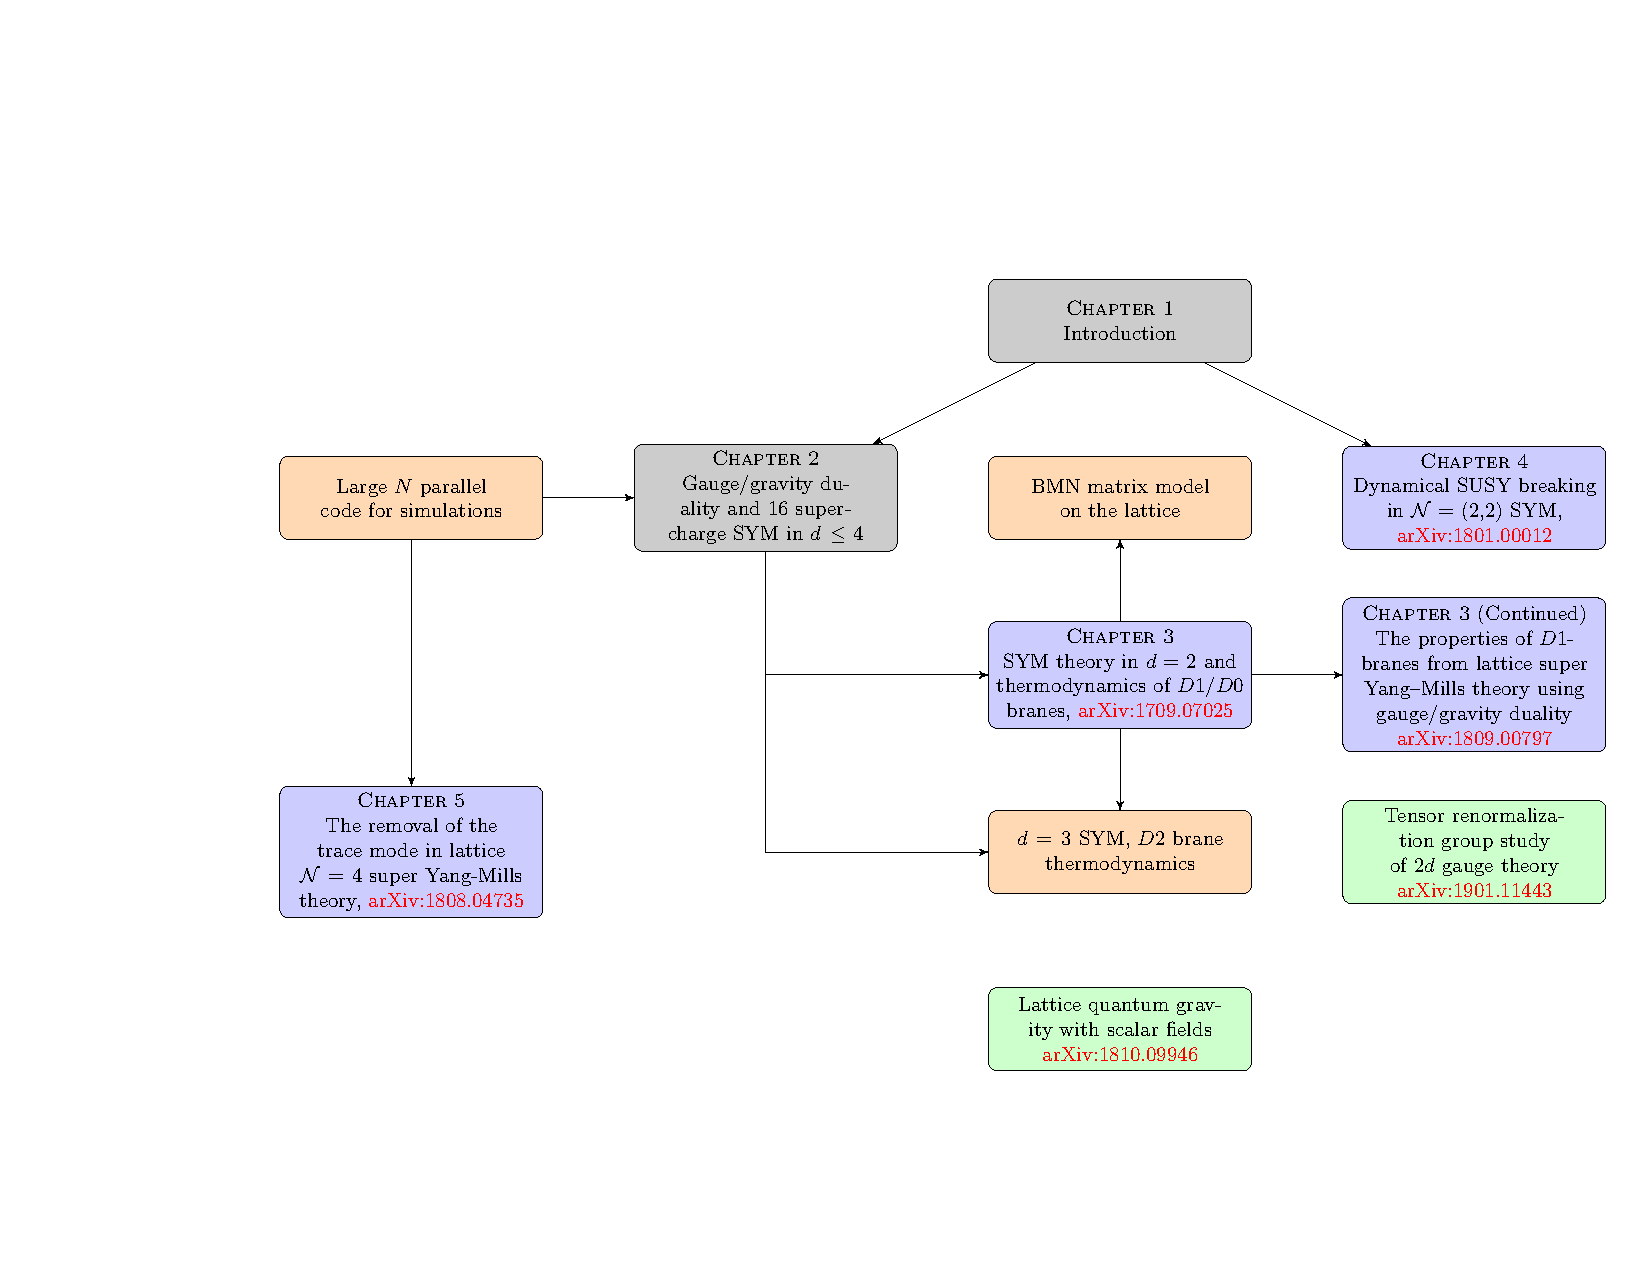
\includegraphics[width=\linewidth]{Figures/Flowchart.pdf}
  \caption{\label{fig:flow1}The grey boxes represent review part of the thesis. The blue boxes are publications that are part of this thesis. The orange boxes represent the work 
which is in progress and expected to be completed in 2019 or later. The green boxes represent publications (journal article/conference proceedings) that were completed 
during the Ph.D. but are not part of this thesis. }
\end{figure}





   
\newpage
    \tableofcontents

 
\newpage    \listoffigures
\newpage    \listoftables

\newpage
     %%%%% calls abstract.tex, ackno.tex, list_pubs.tex, conventions.tex
\mainmatter
\pagenumbering{arabic}


\chapter{\label{ch1}Introduction}
%to lattice supersymmetry
\epigraph{\textit{Simplex sigillum veri (The simple is the seal of the true) \\ 
Pulchritudo splendor veritatis (Beauty is the splendor of truth) } \\ \vspace{3mm} Latin phrase} 

The theory of the renormalization group (RG) flow has been one of the most important ideas in 
Physics in the last century. The fixed points of the RG flow constitute an important class of 
quantum field theories, known as conformal field theories (CFT). 
A conformal field theory is a quantum field theory when the action is invariant under conformal transformations. 
The conformal invariance highly constrains the field theory and has far-reaching implications such as vanishing of 
the energy-momentum tensor. However, in some cases, a quantum process can break this symmetry and give rise 
to trace anomaly and non-zero stress tensor. The CFT can then be completely described by central charges of the 
energy-momentum tensor. These central charges determine the correlation functions of the theory and also 
reorient the theory under renormalization group flow. It is known in two dimensions from 
Zamolodchikov's c-theorem \cite{Zamolodchikov:1986gt} that the central 
charge $c$ increases from the infrared (IR) to the ultraviolet (UV). 
This theorem orders a CFT and provides interpretation of the central charge as
a measure of the field degrees of freedom in the theory. These degrees of freedom decrease along the renormalization
flow due to the decoupling of massive modes. The study of CFTs has also become 
important in recent years due to the holographic application via the AdS/CFT correspondence. 
The results for the entanglement entropy obtained from CFT in lower dimensions agree 
with the calculations using gravity. 

However, it is highly unusual for any theory to have a line 
of fixed points all along the RG flow and to be conformal under quantum interactions. 
One such special theory is $\mathcal{N}=4$ super Yang-Mills (SYM) theory in four dimensions. 
This theory is maximally supersymmetric and has sixteen supercharges. 
This feature is because of supersymmetry\footnote{A non-supersymmetric theory 
which shows this behavior of line of fixed points is XY 
model in two dimensions for $T \le T_{KT}$}. Since this is such an interesting theory, one desires to understand its 
properties non-perturbatively as well. This motivation has resulted in several decades of work realizing 
supersymmetry on the lattice which furnishes a gauge-invariant regularization to study the theory at 
strong couplings. $\mathcal{N}=4$ SYM
is also special because it takes part in the AdS/CFT correspondence, the first concrete example of a 
holographic correspondence between supersymmetric gauge theory and a gravity theory on anti-de Sitter (AdS)
spacetime \cite{Maldacena:1997re, Itzhaki:1998dd, Aharony:1999ti}. 
For a nice discussion on the relation between lattice gauge theory and AdS/CFT correspondence, 
see \cite{Caselle:2000tn}.

The non-perturbative features of supersymmetric Yang-Mills (SYM) is also 
thought to play a crucial role in beyond 
Standard model (BSM) Physics and in M/String theory. 
The non-perturbative study of string theory is based on various matrix models. 
In general, two kinds of non-perturbative formulations of M/string theory exists. 
The \textit{first} is called the Matrix theory. Typical examples are BFSS Matrix model and the
plane-wave Matrix model (PWMM) which describes a sector
of M theory in the infinite momentum frame \footnote{Note that this is
also sometimes called light-cone gauge quantization} on a flat
background and a pp-wave background, respectively. There is another 
0+0-dimensional matrix model called IKKT model \cite{Ishibashi:1996xs}
studied with motivations for applications to string theory. We will not say anything about this 
model in this thesis. These matrix models are dual to classical supergravity only in the large $N$ 
and strong coupling limit which is in general not analytically solvable. In the last ten years, there have 
been several precision numerical calculations which have reproduced predictions from the dual gravity, 
hence providing very strong evidence about the validity of the holographic conjecture, 
which we will discuss in detail in Chapter \ref{ch3}. The BFSS matrix model 
(like many extended supersymmetric models) has a moduli space. 
The moduli space in this theory is given by the eigenvalues of nine commuting matrices i.e. 
$ [X_{i}, X_{j}] = 0 $ that transform under the SO(9) R-symmetry. 
The existence of these flat directions means that, at finite temperature,
the partition function is formally divergent, and it was shown that when Monte
Carlo simulations of this theory are performed, this divergence eventually causes the
simulation to break down. However, at large $N$, we can still understand the
thermodynamics in a meta-stable vacuum state with sufficient precision. 

The \textit{second} non-perturbative approach to string theory/M-theory 
is through the AdS/CFT correspondence. It was first studied by Maldacena for which the pair system was 
Type IIB supergravity on AdS$_5 \times S_5$ and $\mathcal{N}$ = 4 SYM.
Using this duality, several results for the strongly coupled field theory have been reproduced by the classical 
gravity in the bulk. However, the other direction, $\emph{i.e.}$
getting results for gravity from field theory has been less explored because of lack of calculational tools in 
the strongly coupled field theory. This thesis attempts to explore this side of duality by using lattice as a tool for 
dealing with strongly coupled field theory. 
In addition, lattice also provides a window into the finite-$N$ and coupling corrections to the leading holographic 
result only valid in $N \to \infty$ and $\lambda \gg 1$. This is shown in more detail in Figure \ref{fig:Nlam1}. 


\begin{figure}
\begin{center}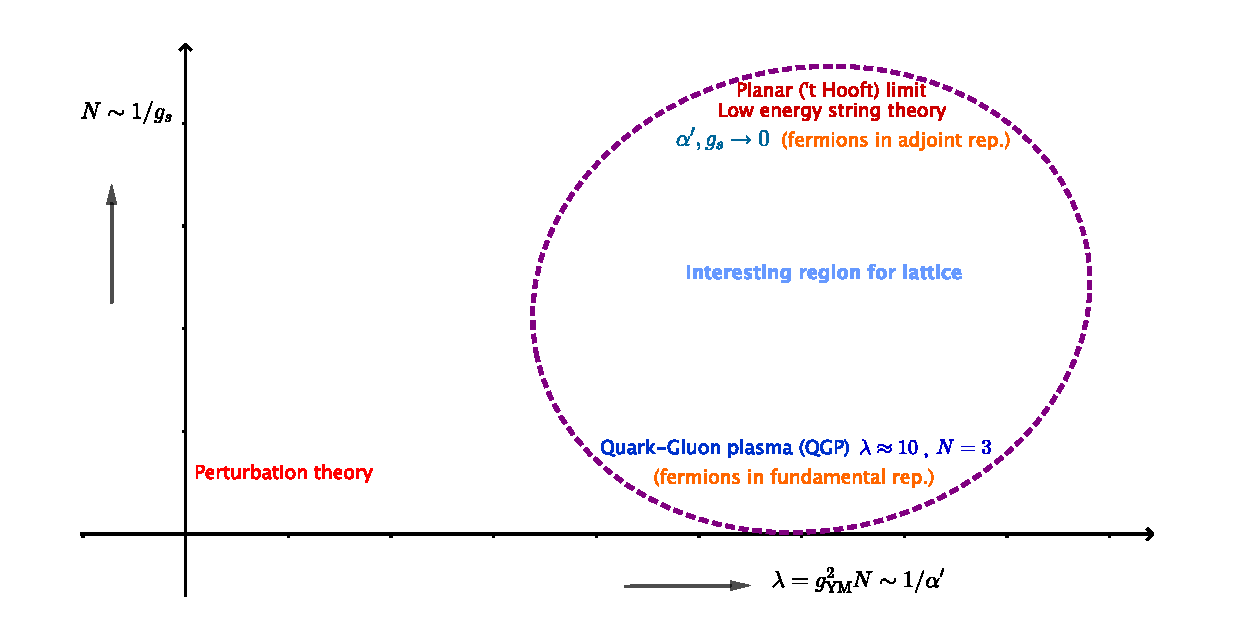
\includegraphics[width=0.85\textwidth]{./Figures/N_lam_phase.pdf}\end{center}
\caption{\label{fig:Nlam1}Different regions of supersymmetric/non-supersymmetric gauge theories in the $N-\lambda$ plane}. 
\end{figure}

\section{Supersymmetry (SUSY)}

Supersymmetry is a theoretical idea which relates half-integer (fermions) and
integer-spin (bosons). For a nice review on supersymmetry and its lattice constructions, 
see \cite{Argyres:2001eva, Seiberg:1997ax, Catterall:2009it}. 
The roots of supersymmetry were laid down when Coleman and Mandula (CM) proved a theorem ~\cite{Coleman:1967ad} 
which was then supposed to be the final nail in the discussion of how the Poincare group and internal symmetries can 
be mixed together. 
They showed that under some assumptions, there was no non-trivial way of combining the two. In a way, it meant that 
there cannot be any manner in which the fermions can be brought on the same footing as bosons. But, then, physics 
thrives on crisis and exceptions. A few years later, Haag, Lopuszanski and Sohnius ~\cite{Haag:1974qh} showed that 
if some of the assumptions in the Coleman-Mandula theorem are relaxed then it is possible to mix these symmetries. 
This implied the use of graded Lie algebra instead of the normal Lie algebra which was used in the argument by CM.  

\subsection{Extension of the space-time symmetry group} 
The Poincare group is composed of transformations of the form, 
\begin{equation}
x^{\mu} \rightarrow x^{\prime \mu} = \Lambda^{\mu}_{\hspace{1mm} \nu} x^{\nu} + a^{\mu}
\end{equation}

We talk about Lorentz transformations if in the above transformation we do not have the $ a^{\mu}$ part. Hence, it is pretty obvious to
imagine Poincare transformations as a direct product between Lorentz transformations and group of 4-translations. 
In fact, it is not a direct but semi-direct product of two. 
The Poincare algebra is given by, 
 
 \begin{equation}
 [M^{\mu\nu} , M^{\rho\sigma}] = i \left (M^{\mu\sigma} \eta^{\nu\rho} + M^{\nu\rho} \eta^{\mu\sigma} - M^{\mu\rho} \eta^{\nu\sigma} - M^{\nu\sigma} \eta^{\mu\rho} \right)
 \end{equation}
 
 \begin{equation}
[P^{\mu}, P^{\nu}] = 0
 \end{equation}
 
\begin{equation}
[M^{\mu\nu}, P^{\sigma}] = i \left(P^{\mu}\eta^{\nu\sigma} - P^{\nu}\eta^{\mu\sigma}\right)
\end{equation}
here $\textbf{M}$ is the anti-symmetric generators of the Lorentz group and $ \textbf{P}$ are the translation generators. 

The CM theorem clearly meant that there was no non-trivial way of mixing particles with integer and half-integer spin. 
Wess and Zumino discovered field theoretic models with this extended symmetry (called 'supersymmetry') 
which connects Bose and Fermi fields and are generated by charge transforming like spinors under the 
Lorentz group (supercharges). These supercharge give rise to a new system of commutation and anti-commutation relations, 
which is not precisely a Lie algebra but a graded algebra. This has a $ \mathcal{Z}_{2}$ grading. 
The Poincar\'{e} generators $ P^\mu$ and $M^{\mu\nu}$ are bosonic generators. In supersymmetry, we add fermionic generators $Q_{\alpha}^{L}$, $\overline{Q_{\beta}^{M}}$, where
$L, M = 1,2, \cdots \mathcal{N}$. The $\mathcal{N} = 1 $ case is simple supersymmetry and $\mathcal{N}  > 1$ is extended supersymmetry. 
The complex spinorial generators follow the following algebra, 

\begin{equation} 
\{Q_{\alpha}^{L}, Q_{\beta}^{M}\} = \epsilon_{\alpha\beta} Z^{LM}
\end{equation} 

\begin{equation} 
 [P,Q] = 0
 \end{equation} 

\begin{equation} 
[Q_{\alpha}^{L}, M_{\mu\nu}]  = \frac{1}{2} (\sigma_{\mu\nu})_{\alpha} \hspace{1mm} ^ {\beta} Q_{\beta}^{L} 
 \end{equation} 

\begin{equation} 
 \{Q_{\alpha}^{L}, \overline{Q_{\beta}^{M}}\} = \delta^{LM} \sigma^{\mu}_{\alpha\beta} P_{\mu}
  \end{equation} 

The last one is the most interesting of these four. It roughly means that the supersymmetric generators are
the square root of the four-momentum. It also means that combining two supersymmetric transformations 
(one of each helicity) corresponds to space-time translation. 
This commutation relation should be enough to dissuade one from attempting to put supersymmetry on the lattice since 
infinitesimal translations don't exist on the lattice and supersymmetry is broken at the classical level. If supersymmetry is 
not consistent with lattice discretization, then one immediately asks - why do we really want to study lattice supersymmetry? 

Supersymmetry is interesting because it is a mathematically consistent and elegant theory. It is worth investigating because
of the relation between SYM theories and string theory and quantum gravity. 
Most of the features of SYM theories are at strong coupling, where we have only a handful of methods in general. 
In order to have a valid non-perturbative definition from first principles, it would be desirable to go back to the highly 
successful tool of lattice gauge theory which has produced amazing results in QCD. 
However, supersymmetry is very different from QCD and has a much richer structure and field content. 
One can immediately see this from supersymmetric algebra, which is very constrained. 
Once we fix the maximum helicity (which for theories without gravity is one, and with gravity is two), 
there are only a few possibilities for the number of supercharges (or supersymmetries) that can exist. In case of no gravity, 
the maximal number of supercharges is 
16 and for supergravity theories, it is 32. If the SYM theory possesses sixteen supercharges, 
we often refer to it as ~`maximally supersymmetric'.
The restriction on the maximal spin comes from the idea that the theory should be renormalizable.
A supersymmetric theory is often labeled with $\mathcal{N}$, $\mathcal{Q}$, $d$  which stands for the 
number of copies of supercharges, number of supercharges, and space-time dimension. 
For ex: $\mathcal{N}=4$ SYM theory in $d=4$ has $\mathcal{Q}=16$ (sixteen supercharges, maximal).
This theory is obtained by dimensional reduction of the ten-dimensional $\mathcal{N}=1$ SYM theory. 

A nice way of deciding which higher-dimensional theory to start from is to count the number of spinor components.  
In ten dimensions, a spinor has $2^{[d/2]} = 32$ complex components which are reduced to 16 real components
after imposing the Majorana-Weyl condition consecutively in that order (which can only be done where d mod $8 = 2$). 
Therefore, $\mathcal{N}=1$ SYM in ten dimensions has 16 real components. 
A Majorana spinor in four dimensions has 4 components. To obtain
$\mathcal{N}=4$ SYM in four dimensions (which has 16 real components) 
one starts with $\mathcal{N}=1$ SYM in ten dimensions just like we mentioned before. 
$\mathcal{N}=1$ SYM in four dimensions similarly has $\mathcal{Q}=4$ components. 
So, in order to construct a supersymmetric theory in two dimensions with four supercharges i.e. $\mathcal{N}$ = (2,2) SYM, 
one needs to start from $\mathcal{N}=1$ SYM in four dimensions. 


\subsection{R-symmetry} 

Supersymmetric theories are endowed with a special symmetry, known as R-symmetry. 
R-symmetry is the symmetry transforming different supercharges in a theory into each other. 
For extended supersymmetry (i.e. $\mathcal{N} > 1$), the R-symmetry group becomes a 
global non-abelian group. The bosonic, fermionic fields and the supercharges form a representation of the 
R-symmetry, as well as Euclidean rotation group $SO(d)_{E}$.
$\mathcal{N}=1$ SYM in four dimensions has a U(1) R
-symmetry while the $\mathcal{N}=1$
SYM in ten dimensions has no R-symmetry. 
When this $\mathcal{N}=1$ SYM in ten dimensions is dimensionally reduced to $d$ space-time 
dimensions, the R-symmetry group is enlarged to $SO(10-d)$ R-symmetry. Hence, we can immediately 
see that $\mathcal{N}=4$ SYM in four dimensions has $SO(6)$ R-symmetry.
Note that this $SO(6)$ R-symmetry is exactly the same as isometries of $S^{5}$ (five-sphere) 
which takes part in the AdS/CFT correspondence. 
In our quest to understand supersymmetry on the lattice, we will now briefly review
the ideas that will be important in constructing the lattice formulation of supersymmetric theories
which preserves some subset of the supersymmetries. 



\subsection{Topological Field Theories (TFT)}

Before discussing the lattice formulation of the supersymmetric gauge theories, we will review
the idea of topological field theory which plays an important role in lattice theory. 
One of the easiest ways to construct a topological field theory is to 
take an extended space-time supersymmetric theory and \textit{twist} it. A common feature of both supersymmetric lattice
theories and topological field theories is the presence of nilpotent scalar supercharge $\mathcal{Q}$. 
They have actions which are $\mathcal{Q}$-exact. 
All the supersymmetric lattice theories are associated with topological field theories but the opposite is not always true. 
A topological field theory (TFT) is characterized by the following:
\vspace{3mm} 
\begin{itemize}
\item Collection of fields defined on a Riemannian manifold($\textbf{$\mathcal{M}$}$,g)
\item A nilpotent operator which is Grassmann odd
\item Physical states are in Q-cohomology class \footnote{Given the second condition above that the operator should 
be nilpotent means that it is satisfied when a particular state is annihilated by that operator (let's call it Q). Such states 
are said to be in the kernel of Q. Alternatively, a state which is annihilated by Q can take a form of Q acting on something, 
such states are said to be in the image of Q. But, there may be some states which are in the kernel of Q, but not in the image; 
such states are said to be in the cohomology of Q.} 
\item Energy-momentum tensor is Q-exact i.e. \[ T_{\mu\nu} = Q G_{\mu\nu} \]
\end{itemize}

Q is referred to as ~`BRST charge' (also BRST operator) and the Grassmann grading corresponds to the ghost number. 
In general, Q is metric independent and is the simplest situation. However, there are far more interesting cases 
where $T_{\alpha\beta}$ is a BRST commutator even when Q fails to be metric independent. There also exist cases 
where $T_{\alpha\beta}$ is not even a BRST commutator, though, it is possible even then, sometimes, to establish the
topological nature. Consider the change in the partition function, 
\begin{equation}
Z = \int \mathcal{D} \phi e^{-S_{q}}
\end{equation}
under an infinitesimal change in the metric, we get :
\begin{align}
\delta_{g} Z&= \int \mathcal{D} \phi e^{-S_{q}} \left(-\frac{1}{2} \int_{M} d^{n} x 
\sqrt{g} \delta g^{\alpha\beta} T_{\alpha\beta}\right)\\
&=\int \mathcal{D} \phi e^{-S_{q}} \left(-\frac{1}{2} \int_{M} d^{n} x 
\sqrt{g} \delta g^{\alpha\beta} QG_{\alpha\beta}\right)\\
&=\int \mathcal{D} \phi e^{-S_{q}} Q\chi_{\alpha\beta} = \langle Q\chi_{\alpha\beta}\rangle = 0
\end{align}
where, $ \chi = - \frac{1}{2} \int_{M} d^{n}x \sqrt{g} \delta g^{\alpha\beta} G_{\alpha\beta}$. We have 
used the fact that vacuum is BRST invariant. 
This means that the partition function does not depend on the local structure of the manifold: 
Z is a topological invariant. 
Now consider the following action, 
\begin{equation}
S(\phi) = \int d^{d} x \sqrt{g} \left[g^{\mu\nu} \nabla_{\mu} \phi  \nabla_{\nu} \phi \right]
\end{equation}
where $g^{\mu\nu}$ is the Riemannian metric and $\nabla$ is the covariant derivative. We can define the energy-momentum tensor as :
\begin{equation}
T_{\mu\nu} = \frac{\delta S}{\delta g^{\mu\nu}} 
\end{equation}
and rewriting it gives, \footnote{Using the fact that Z is already independent of metric},  
\begin{equation}
\langle T_{\mu\nu} \rangle =  \frac{1}{\mathcal{Z}}\int \mathcal{D} \phi \hspace{1mm} \left(\frac{\delta S}{\delta g^{\mu\nu}}\right) \exp\left[\frac{-S(\phi)}{\hbar}\right]  
\end{equation}
\begin{equation}
\langle T_{\mu\nu} \rangle= 0
\end{equation}
We have established that the metric variation of the partition function vanishes, and in turn that the energy-momentum tensor is zero. We need to examine the presence of other metric independent correlation functions in the theory. 
Let's start by considering the vacuum expectation value of an observable, 

\begin{equation}
 \langle \mathcal{O} \rangle = \int \mathcal{D} \Phi e^{-S} \mathcal{O}(\Phi)
 \end{equation}
We have to derive the conditions for this change in expectation value to be zero, 
\begin{equation}
\delta \langle \mathcal{O} \rangle = \int \mathcal{D} \Phi e^{-S} (\delta_{g} \mathcal{O} - \delta_{g} S_{q} \cdot \mathcal{O})
\end{equation}
Assume that $\mathcal{O}$ satisfies the following properties :
\begin{equation}
\delta_{g} \mathcal{O} = \{Q, T\}  \hspace{2mm} , \hspace{5mm} \{Q, \mathcal{O}\} = 0
\end{equation}
for some T, we then have :
\begin{equation}
\delta_{g}\langle \mathcal{O} \rangle = \langle \{Q, T + \chi \mathcal{O}\}\rangle = 0
\end{equation}
It is interesting to note that even though $\chi$ depends on $V_{\alpha\beta}$ which contains metric dependence, 
we have wrapped it up in form of BRST commutator and still have metric independence. TFT can be classified into
two types: 1. Schwarz type 2. Cohomological type (Witten-type). 
\begin{itemize} 
\item \textbf{Schwarz Type}: The classical action is explicitly independent of the metric. Chern-Simons theory is a 
prototype of this class of topological field theories introduced by Witten in 1980s. The metric independence implies 
that the classical stress-energy tensor of TFT vanishes. In addition, even the quantum stress-energy tensor vanishes 
because of the fact that the remaining part of quantum action has been recast as a BRST commutator.  
$ \frac{\delta S}{\delta g^{\mu\nu}} = T_{\mu\nu} = 0 $. The alternate cases where the classical action depends 
explicitly on metric is not dealt here. It is also clear from the equation below that the quantum action for Schwarz 
type theories do not enjoy the property that the quantum action is Q-exact. 
\begin{equation}
S_{q}(\phi, g) = S_{c}(\phi) + QV(\phi,g) 
\end{equation}
\item \textbf{Witten Type}: In Witten-type topological field theories, the topological invariance is more subtle. 
The lagrangian generally depends on the metric explicitly, but one shows that the expectation value of the 
partition function and special classes of correlation functions are diffeomorphism 
\footnote{Roughly speaking, this means that they are metric independent} invariant. 
The important characteristic of Witten-type theory is that the quantum action $S_{q}$, 
which comprised the classical action plus all necessary gauge fixing and ghost terms, 
can be written as BRST commutator i.e.,
\begin{equation}
S_{q} = \langle \{Q, V\}\rangle 
\end{equation}
for some functional $V(\phi,g)$ of the fields and Q is nilpotent. 
In BRST quantization of gauge theories, one constructs a BRST operator Q which is nilpotent. 
The variation of any functional $\mathcal{O}$ is denoted by $
\delta\mathcal{O} = \{Q,\mathcal{O}\} $, where the bracket is used to represent the graded commutator 
with the fermionic charge Q. A state which is annihilated by Q is called Q-closed, while a state of the 
form $ Q|\chi\rangle$ is called Q-exact. From the BRST invariance of the vacuum, we can conclude 
that the vacuum expectation value of \{Q,$\mathcal{O}$\} for any functional $\mathcal{O}$ is zero i.e. 
\begin{equation}
 \langle 0 | \{Q,\mathcal{O}\} | 0 \rangle  = 0 
 \end{equation}
An operator of the form \{Q,$\mathcal{O}\}$ is called BRST commutator. The energy-momentum tensor 
$T_{\alpha\beta}$ is defined as the change in the action under smooth deformations of the metric.
\begin{equation}
\delta_{g} S = \frac{1}{2} \int_{M} d^{n} x \sqrt{g} \delta g_{\alpha\beta} T_{\alpha\beta}
\end{equation}
We assume throughout that the functional measure in the path integral is both Q-invariant and metric
independent. If it is not the case, we have to check for metric anomalies which are outside the scope of this thesis. 
\end{itemize} 


\subsection{Twisting of the supersymmetric theory}
In the 1980s, Witten noticed that supersymmetry has a deep relation to topology. 
The simplest example of such a relation is supersymmetric quantum mechanics, 
which provides a physical reformulation of Morse theory. 
Their relation is not obvious because of the degrees of freedom in a topological field theory of 
Witten-type and supersymmetric theory is very different. 
Witten-type theories have no physical degrees of freedom, unlike the supersymmetric theories. 
Their relationship becomes more apparent when we follow a procedure known as ~`twisting'. 
The \textit{twisting} procedure can be viewed as a modification of Lorentz transformation properties. 
This process leads to at least one scalar supercharge, unlike the half-integer supercharges we have before the twisting. 
\textit{Twisting} can be done through in several different ways based on how we embed the spin connection 
in the R-symmetry group of the extended supersymmetric theory. 
In the twisting procedure, one first selects one of the two components of the rotation group and 
then replaces it by the diagonal sum of that component with a SU(2) subgroup of the internal group 
\footnote{So now, for every rotation in Euclidean space, we do a similar rotation in isospin space. 
This is similar to identify the different indices as mentioned in the text}. For the $\mathcal{N}$ = 2 
SUSY in four dimensions, this can be done in only one way. There might be several ways of doing
this twisting depending on how large the R-symmetry group is for that theory.

The new choice of rotation group involved in the twist implies that the isospin index $\textit{i}$ 
becomes a spinorial index $\alpha$ : $ \mathcal{Q}^{i}_{\alpha} \mapsto \mathcal{Q}^{\beta}_{\alpha}$ 
and $\bar{\mathcal{Q}}_{i \beta} \mapsto G_{\alpha\dot{\beta}}$. The trace of $ \mathcal{Q}^{\beta}_{\alpha}$ 
is chosen as the generator of scalar symmetry which we desired since it has many advantages. 
This scalar generator is the relation between supersymmetric theories and TFT's. There are three
 inequivalent twists of the $\mathcal{N}=4$ SYM theory in four dimensions partly due to Yamron, 
 Vafa \& Witten  \& Marcus. Only the last one of these correspond to the orbifold and twisted constructions 
 and will be useful for this thesis. The $\mathcal{N}=4$ SYM theory in $d=4$ dimensions possesses a 
 global Euclidean Lorentz symmetry $SO(4)_{E}$ $\sim SU(2) \times SU(2) $ on $\mathbb{R}^{4}$ 
 and a global R-symmetry group SO(6). 
The R-symmetry contains a subgroup $SO(4)_{R} \times U(1)$. 
To construct the twisted theory, we take the diagonal sum of $SO(4)_{E} \times SO(4)_{R}$ and declare it the new rotation group. 
The $U(1)$ part of the symmetry group is undisturbed and continues to be a global R-symmetry of the twisted theory.
Both bosons and fermions are in the integer spin representations after twisting. They are $p$-form tensors of the 
new rotation group i.e. $SO(d)^{\prime}$. 

\subsection{K\"{a}hler-Dirac fermions and $A_{4}^{*}$ lattice - steps to $\mathcal{Q}$-exact SUSY} 

In a remarkable paper, K\"{a}hler provided a geometric interpretation to fermions in term of inhomogeneous differential forms. 
It meant that Dirac equation for spin-1/2 particles can be written in terms of differential forms. Such fields are called
K\"{a}hler-Dirac (KD) or Dirac-K\"{a}hler fields. The KD equation in four dimensions is, 

\begin{equation}
(\partial - \delta + m) \Phi = 0 
\end{equation}
where $\partial$ is the boundary and $\delta$ is the co-boundary operator and they satisfy, $\partial^2 = \delta^2 = 0$. The Laplacian is then written as,

\begin{equation}
\Box = (\partial - \delta)^{2} = -(\partial \delta + \delta \partial)
\end{equation}

The KD equation is actually equivalent to four copies of the Dirac equation. This mapping makes it possible to represent 
spin-1/2 fermions in terms of bosonic fields. This is to some extent perfectly compatible with the idea of supersymmetry. 
The extra fermion species are a problem in QCD but they are very natural in supersymmetric theories. To fill the entire 
KD multiplet in $d$ dimensions, we need at least $2^d$ fermions. KD fermions can also be thought of as 
staggered fermions familiar from lattice QCD (also known as Kogut-Susskind fermions) with one 
half the lattice spacing obtained by combining the lattice and its dual lattice. 
In the construction of $\mathcal{Q}$-exact lattice supersymmetry, these KD fermions play a very important role. 
The fermions of the twisted theory are no longer spinors but anti-symmetric tensor fields which are consistent with 
their interpretation as KD fermions. However, it is required that this mapping fills the entire KD multiplet and that 
highly restricts the class of theories for which one can do this. In addition to the topological twisting 
and the idea of K\"{a}hler-Dirac fermions described above, the requirement of 
exact lattice supersymmetry also needs highly symmetric lattices to target the correct continuum theory. 
With a greater symmetry of the spacetime lattice, we expect fewer relevant or marginal operators.  

One such highly symmetric lattice in four dimensions is already known as $A_{4}^{*}$. 
It is also sometimes called the dual of the 4-simplex lattice.
This lattice has five links which are associated with five complex valued fields which include the six scalars and four gauge 
fields of the $\mathcal{N}=4$ SYM theory. This lattice treats all the five gauge links (bosonic variables) equally 
and preserves $S_{5}$ permutation symmetry. This $S_{5}$ symmetry \footnote{In this thesis, $S_{5}$
is also used to refer to five-sphere, the difference should be clear from the context.} provides a set of irreducible representations 
that match exactly those of the continuum twisted SO(4) symmetry (discussed in the previous section). Note that the 
lattice point group in supersymmetric lattices cannot be considered to be a subgroup of just the Lorentz group, 
but rather it is a subgroup of the product of the Lorentz group and the R-symmetry group, which in the same as the 
twisted SO(4) group. There might be some implications of the fact that what is preserved on the lattice is not 
the entire SO(6) R-symmetry group but only some subgroup of it. This is not clear to the author at the moment 
and will not be addressed any further in this thesis. 

\section{$\mathcal{N} = 4 $ SYM in $d=4$}

The most extensively studied of all SYM theories is $\mathcal{N} = 4 $ SYM in $d=4$. 
The theory has a coupling constant which does not run and is conformal. 
It can be thought of as the most symmetric theory in four dimensions without gravity. 
This theory can be obtained by dimensionally reduce the d=10 $\mathcal{N} = 1 $ SYM down to 
four dimensions. This theory possesses SO(6) R-symmetry inherited from the reduced directions of the Lorentz symmetry of 
the $d=10$ dimensional theory before reduction. The field content of the theory is six scalars, 
and sixteen fermionic matrices in the adjoint representation of the gauge group SU($N$).  
Supersymmetry and conformal symmetry in $\mathcal{N} = 4 $ SYM leads
to even bigger symmetry group, due to the fact that supersymmetry and
special conformal transformations do not commute. 
The entire group is known as the superconformal (SC) group and is given by
the supergroup $SU(2, 2|4)$. 

\subsection{Dimensional reduction from ten dimensions} 
We start with a super-Yang-Mills theory in ten dimensions, where the action is, 
\begin{equation}
S_{\mathcal{N} = 1} = \frac{1}{g^2} \int d^{10} x ~ \mathrm{Tr} \Bigg (-\frac{1}{4} F_{MN}F^{MN} +\frac{i}{2} \Psi \slashed{D} \Psi \Bigg) 
\label{eq:10-dim} 
\end{equation}
where $F_{MN}$ is the ordinary field strength constructed out of the vector in the multiplet
and $\Psi_{a}$ is the Majorana-Weyl spinor with $a$ taking values from 1 to 16. Both are in the 
adjoint representation of the gauge group. We define $ \slashed{D} = \Gamma D $, where
$ (D_{\mu} \Psi)^{a} = \partial_{\mu} \Psi^{a} + g f^{a}_{bc} A_{\mu}^{b} \Psi^{c}$. 
The supersymmetric transformations ($\delta_{\epsilon}$) which leave ~\ref{eq:10-dim} invariant are given by, 
\begin{equation}
\delta_{\epsilon} A_{\mu}^{a} = \frac{i}{2} \bar{\epsilon} \Gamma_{\mu} \Psi^{a} 
\end{equation} 
\begin{equation}
\delta_{\epsilon} \Psi^{a} = -\frac{1}{4}F_{\mu\nu}^{a} \Gamma^{\mu \nu} \epsilon
\end{equation}
\begin{equation}
\delta_{\epsilon} \overline{\Psi}^a = \frac{1}{4} \overline{\epsilon} F_{\mu\nu}^{a} \Gamma^{\mu \nu} 
\end{equation}
where $\epsilon$ with index suppressed denotes infinitesimal SUSY parameter (multiplying 
some SUSY generator). One important point to note is that the Dirac spinor has $2^{D/2}$ \emph{i.e.} 
32 complex components. 
In space-time dimensions, $d$ where $ d ~ \text{mod} ~ 8 = 2$, we can have 
Majorana-Weyl representation (see appendix for the table). Majorana (or reality) condition reduces the 
32 complex components to 32 real components, and the Weyl condition reduces this further to 16 real components. 
Hence, in this case, we have sixteen real components of Majorana-Weyl spinor components or eight complex components
which equals the bosonic degrees of freedom. Thus, it is evident that supersymmetry of 
~\ref{eq:10-dim} also rests on the fact that $D-2$ has to equal some power of 2, 
which picks out $D=3,4,6$ and $10$ as possible options. For most of our purposes, 
we will only consider reductions from $D=10$. 
We can dimensionally reducing the theory from ten dimensions down to four dimensions 
using the idea of compactification assuming no motion along the reduced six directions. 
The reduced gauge degrees of freedom the ten-dimensional theory 
behaves as scalars $X_{i}$, where $ i = 1 \cdots 6$. The field tensor $F_{MN}$ breaks as,  

\begin{equation}
F_{AB} = -i[X_{A}, X_{B}] 
\end{equation}

\begin{equation}
F_{\mu A} = \partial_{\mu} X_{A} -i [A_{\mu}, X_{A}]  = D_{\mu} X_{A} 
\end{equation}
and, 
\begin{equation}
F_{\mu \nu} = \partial_{\mu} A_{\nu} - \partial_{\nu} A_{\mu} -i [A_{\mu}, A_{\nu}] 
\end{equation}
The kinetic term of ~\ref{eq:10-dim} splits as, 
\begin{equation}
-\frac{1}{4} F_{MN}F^{MN} = -\frac{1}{4} F_{\mu\nu}F^{\mu\nu} + \frac{1}{2} \sum_{I} (D_{\mu} X_{I})^{2}   - \frac{1}{4} \sum_{A,B} [X_{A}, X_{B}]^{2} 
\end{equation}
The fermions are split according to, 
\begin{equation}
\frac{i}{2} \Psi^{n} \slashed{D} \Psi_{n} = \frac{i}{2} \Psi^{\mu} \slashed{D} \Psi_{\mu} + \frac{1}{2} \Psi \Gamma^{A}[X_{A}, \Psi] 
\end{equation}
where the second term is the Yukawa term in the four-dimensional theory. 

For a non-Abelian SU(N) gauge theory, the one-loop $\beta$ 
function for the gauge coupling $g_{YM}$ is given by \cite{Gross:1973ju, 2012LMaPh..99...33M}
 \begin{equation}
\beta(g_{YM}) = \mu \frac{\partial g_{YM}}{\partial \mu} = \frac{-g_{YM}^{3}}{16 \pi^{2}} \left ( \frac{11}{6}T_{adj} - \frac{1}{12} \sum_{s} T(r_{s}) - \frac{1}{3} \sum_{f} T(r_{f}) \right) 
\end{equation}
 where the sum over $s$ is over real scalars (six of these) and $f$ is over 
real fermions and $T(r)$ is the index of representation $r$. 
Since everything here is in adjoint representation, we can simplify it as, 
\begin{equation}
\beta(g_{YM}) = -\frac{g_{YM}^{3}}{16\pi^{2}}\frac{T_{adj}}{6}\left(11 - \frac{N_{s}}{2} - 2N_{f} \right) 
\end{equation}
hence, this is zero for $\mathcal{N} = 4 $ SYM since $N_{s} = 6$ and $N_{f} = 4$. 
 
\subsection{Some properties of $\mathcal{N} = 4$ SYM.} 
 $\mathcal{N} = 4$ SYM possesses flat directions corresponding to $ [X_{i}, X_{j}] = 0$, when the scalars $X$ belong to the 
 Cartan sub-algebra of the gauge group SU($N$). This leads to a moduli space of vacuum solutions. The section of moduli space where only the adjoint scalars of 
 $\mathcal{N} = 4$ SYM get a vacuum expectation value (VEV) is referred to as 
the Coulomb branch. The VEV can at most Higgs the gauge group down to 
U(1) (where the U(1) is intact) and this implies that the branch can still 
support long-distance EM forces (a bunch of copies of electromagnetism) 
and free photons since the U(1) gauge fields are still massless. 
The VEV of the scalars give a mass scale to the otherwise conformal 
$\mathcal{N} = 4$ SYM at the superconformal fixed point
and this symmetry is broken and so is the gauge symmetry. The process of 
Higgsing from $U(N)$ to $U(1)^{N}$ gives W-bosons a mass which 
just depends on $ m_{W}^{ab}  = |x_a - x_b | = Z_{ab} $, where $Z_{ab}$ is the central charge of the BPS objects. 
Note that W-bosons are 1/2-BPS objects with respect to the some still-unbroken $\mathcal{N} = 4$ SYM. 
This also has a nice interpretation in terms of D-branes via the AdS/CFT duality which can be found in the standard 
gauge/gravity review \cite{Aharony:1999ti}. This theory also has S-duality under which:
\[ \tau_{YM} = \frac{\theta}{2\pi} + i \frac{2\pi}{g^{2}_{YM}} \]
goes to $ -1/\tau$, where we have defined the 't~Hooft coupling $ \lambda = g_{YM}^{2} N $. 


\subsection{\label{sec:latticeN4}Lattice  $\mathcal{N} = 4$ SYM}
The continuum $\cN = 4$ SYM theory can be twisted in three different ways to construct topological field theories.
For our purposes, the maximal twisting ~\cite{Marcus:1995mq} would be required to have maximum overlap with the original 
R-symmetry group. This twist is sometimes also called the GL-twist (role in Geometric Langlands program). 
In this subsection we briefly mention this twisted theory and its implementation on the $A_4^*$ lattice, this will be 
further discussed with numerical results in Chapter \ref{ch5}. 
We review this construction here, details can be found in ~\cite{Kaplan:2005ta, Catterall:2009it}
The main idea of the maximal twist is to form the complex combination
\beq
  \label{4dgauge}
  \cA_\mu \equiv A_{\mu} + iB_{\mu},
\eeq
where $A_{\mu}$ are the usual four-dimensional gauge fields and $B_{\mu}$ is a vector formed out of four of the six adjoint scalars $\Phi_{IJ}$ of the $\cN = 4$ theory.
The two remaining scalars remain singlets after twisting process.
The four Majorana fermions ($\Psi^I$ and their partners $\Psi^c_I$) are regrouped into an anti-symmetric tensor $\chi_{\mu\nu}$, 
two vectors $\psi_\mu$ and $\bar{\psi}_{\mu}$ and two scalar components $\eta$ and $\bar{\eta}$, altogether 16 single components.
We combine the four gauge fields and six scalars in five links spanning directions in the $A_{4}^{*}$ lattice. 

\beq
  \label{5dgauge}
  \cA_a \equiv A_a + iB_a,
\eeq
where the index ~`$a$' runs from $1, \cdots, 5$.
We assign the two singlet scalars to the new fifth component $\cA_5$.
Similarly, the 16 fermion fields can be regrouped into the multiplet $\chi_{ab}, \psi_a, \eta$, with $\chi_{ab}$ anti-symmetric.
We can then introduce complexified field strengths,
\begin{align}
  \cF_{ab} & \equiv [\cD_a, \cD_b] &
  \cFb_{ab} & \equiv [\cDb_a, \cDb_b],
\end{align}
where the corresponding complexified covariant derivatives read
\begin{align}
  \cD_a & = \partial_a + \cA_a &
  \cDb_a & = \partial_a + \cAb_a.
\end{align}
One scalar supersymmetry charge $\cQ$ becomes nilpotent after the twisting.
These act as follows:
\begin{align}
  & \cQ\; \cA_a = \psi_a         & & \cQ\; \psi_a = 0                       \cr
  & \cQ\; \chi_{ab} = -\cFb_{ab} & & \cQ\; \cAb_a = 0 \label{BRSTsymmetry}  \\
  & \cQ\; \eta = d               & & \cQ\; d = 0,                           \nn
\end{align}
where $d$ is an auxiliary field with equation of motion $d = \left[\cDb_a, \cD_a\right]$ (repeated indices summed).
The other fifteen supersymmetry charges are twisted into a vector $\cQ_a$ and anti-symmetric tensor $\cQ_{ab}$.
Except for a topological $\cQ$-closed term,
\beq
  \label{closed}
  S_{\rm cl} = -\frac{1}{16g^2} \int \Tr \epsilon_{mnpqr} \chi_{qr} \cDb_p \chi_{mn},
\eeq
the full $\cN = 4$ action can be written in $\mathcal{Q}$-exact form, 
\beq
  \label{4daction}
  S = \frac{1}{4g^2} \cQ \int \mbox{Tr}\left[\chi_{ab}\cF_{ab} + \eta [ \cDb_a,\cD_a ] - \frac{1}{2}\eta d\right] + S_{\rm cl}
\eeq
where $\mathcal{Q} S_{\rm cl} = 0$ is ensured by the Bianchi identity.

As explained in detail in Ref.~\cite{Catterall:2007kn}, this twisted formulation leads naturally to a lattice construction of the theory.
In fact, there is a very direct and geometric prescription for how to map continuum variables 
(covariant derivatives and tensor fields of arbitrary rank) to those of the 
lattice~\cite{Catterall:2007kn, Damgaard:2008pa}.
In this particular case, the lattice inherits the five-component language, and is most 
naturally represented as the $A_4^*$ lattice with manifest $S_5$ point group symmetry 
in four space-time dimensions.
The basis vectors of the $A_4^*$ lattice link the center of an equilateral 4-simplex to each of its five vertices.
This is the analog of the triangular lattice in two dimensions. 

In terms of the complex link variables $\cU_a(\vn)$, and the finite difference operators
\begin{align}
  \cD^{(+)}_a f_b(\vn) & = \cU_a(\vn)f_b(\vn + \hatbmu_a) - f_b(\vn)\cU_a(\vn+ \hatbmu_b)                                       \cr
  \cDb^{(-)}_a f_a(\vn) & = f_a(\vn)\cUb_a(\vn) - \cUb_a(\vn - \hatbmu_a)f_a(\vn - \hatbmu_a)                                   \\
  \cDb_c^{(-)} f_{ab}(\vn + \hatbmu_c) & = f_{ab}(\vn + \hatbmu_c) \cUb_c(\vn + \hatbmu_a + \hatbmu_b) - \cUb_c(\vn)f_{ab}(\vn) \nn
\end{align}
from Refs.~\cite{Catterall:2007kn, Damgaard:2008pa}, the lattice action can be written down by transcribing the continuum action:
\begin{align}
  \label{SlatQ}
  S_0 & = \frac{N}{4\lambda_{\rm lat}} \sum_{\vn} \mathrm{Tr}  \mathcal{Q} \left(\chi_{ab}(\vn)\cD_a^{(+)}\cU_b(\vn) + \eta(\vn) \cDb_a^{(-)}\cU_a(\vn) - \frac{1}{2}\eta(\vn) d(\vn) \right) + S_{\rm cl} \\
  S_{\rm cl} & = -\frac{N}{16\lambda_{\rm lat}} \sum_{\vn} \mathrm{Tr} \epsilon_{abcde} \chi_{de}(\vn + \hatbmu_a + \hatbmu_b + \hatbmu_c) \cDb^{(-)}_{c} \chi_{ab}(\vn + \hatbmu_c).
\end{align}
Here $\lambda_{\rm lat} = g_{\rm lat}^2 N$ differs from the continuum 't~Hooft coupling by a 
normalization factor of $1 / \sqrt{5}$. 
On the lattice $S_{\rm cl}$ is $\cQ$-closed on account of a lattice analog of the continuum 
Bianchi identity~\cite{Catterall:2007kn},
\begin{equation}
  \epsilon_{abcde} \cDb^{(-)}_c \cFb_{ab}(\vn + \hatbmu_c) = 0.
\end{equation}

The physical observables are those of the untwisted theory to which we can always map back.
It is expected that in flat space-time this twisting retains the important features 
of the theory (at least vacuum states), 
while for general curved background, it is a different theory. 
Expanding the action (\ref{SlatQ}), ,
\begin{align}
  & \cQ\; \cU_a = \psi_a          & & \cQ\; \psi_a = 0 \nn \\
  & \cQ\; \chi_{ab} = -\cFb_{ab}  & & \cQ\; \cUb_a = 0 \label{BRSTlatticesymmetry} \\
  & \cQ\; \eta = d                & & \cQ\; d = 0, \nn
\end{align}
and integrating out the auxiliary field $d$ one obtains
\begin{equation}
  \label{eq:lat_act}
  \begin{split}
    S_0 & = \frac{N}{4\lambda_{\rm lat}} \sum_{\vn} \mbox{Tr}\left[-\cFb_{ab}(\vn) \cF_{ab}(\vn) + \frac{1}{2}\left(\cDb_a^{(-)}\cU_a(\vn)\right)^2 \right. \\
        & \qquad\qquad\qquad\qquad\qquad\qquad\qquad \left. - \chi_{ab}(\vn) \cD^{(+)}_{[a}\psi_{b]}(\vn) - \eta(\vn) \cDb^{(-)}_a\psi_a(\vn)\right] + S_{\rm cl}.
  \end{split}
\end{equation}
In order to stabilize numerical computations we regulate the flat directions by
 including in the lattice action a potential, 
\begin{equation}
  \label{eq:mass}
  S = S_0 + \frac{N}{4\lambda_{\rm lat}} \mu^2 \sum_{\vn,\ a} \left(\frac{1}{N}\mbox{Tr}\left[\cUb_a(\vn) \cU_a(\vn)\right] - 1\right)^2,
\end{equation}
with $\mu$ a ~`bosonic mass' parameter to lift the flat directions. 
This non-zero $\mu$ softly breaks supersymmetry, which we 
extrapolate to zero most of the time. 
The full lattice action is invariant under lattice gauge transformations,
\begin{align}
  \cU_a(\vn) & \to G(\vn)\cU_a(\vn)G^{\dag}(\vn+\hatbmu_a)                   &
  \psi_a(\vn) & \to G(\vn)\psi_a(\vn)G^{\dag}(\vn+\hatbmu_a)                 \\
  \chi_{ab}(\vn) & \to G(\vn+\hatbmu_a+\hatbmu_b)\chi_{ab}(\vn)G^{\dag}(\vn) &
  \eta(\vn) & \to G(\vn)\eta(\vn)G^{\dag}(\vn),                              \nn
\end{align}
where $G \in$ U($N$).
These transformation rules are as expected for lattice variables in the adjoint representation.
The gauge links are expanded in generators of the $\mathfrak u(N)$ algebra with complex coefficients
therefore becoming elements of the algebra $\glN$.

\beq
  \cU_a(\vn) = \sum_{C = 1}^{N^2} T^C\cU^C_a(\vn)
\eeq

To obtain the correct naive continuum limit, the complexified gauge links must have the 
expansion $\cU_a(x) = \Ibb + \cA_a(x) + \dots$ in some appropriate gauge. 
In Chapter \ref{ch5}, we discuss how to deal with the $U(1)$ trace mode in the 
lattice construction to target the correct continuum limit. 

\chapter{\label{ch2}Large $N$ limit and holographic dualities}
\epigraph{\textit{To them, I said, 
the truth would be literally nothing 
but the shadows of the images....} \vspace{3mm} \\ Plato, The Republic (Book VII)}  

\section{Large $N$ limit of gauge theories}

The theory of strong interactions, QCD, has a gauge group SU(3). In order 
to understand QCD 't~Hooft introduced 
\cite{Hooft:1974aa, SCA} the idea of the large $N$ limit of 
gauge theories by considering a $SU(N)$ gauge group. 
We often associate more variables with greater complexity. But this is not always true. 
There are many classes of theories which simplify in the large $N$ limit. 
This occurs because the fields are related by a certain
symmetry which ensures that the collective behavior of the fields becomes more constraining 
as their number increases. This is in some sense similar to the classical limit. The resulting
coupled degrees of freedom typically look different from the Lagrangian of the initial theory. 
It was realized early on that the large $N$ limit of gauge theories is also related to string theory 
because roughly speaking in the large $N$ limit one sums over surfaces of different genus and in 
string theory one sums over different world-sheet topologies. 
The idea of large $N$ has been a very fruitful area of research for decades 
now. Some developments include factorization equations, large $N$ phase transitions, 
Eguchi-Kawai (EK) volume reductions, holography, and AdS/CFT correspondence. 
The EK model ~\cite{Eguchi:1982nm} was proposed on the basis of large $N$ factorization of 
Wilson loops based on the analysis of Migdal-Makeenko 
~\cite{Makeenko:1979pb} \cite{Makeenko:1980vm} 
loop equations (the Schwinger-Dyson equations for Wilson loop
correlation functions) and assuming that the center symmetry ($\mathbb{Z}_{N}$) was unbroken. 

In QCD, one might think that the expansion parameter is $g_{YM}$, but this is not true in the light of the 
renormalization group equations. QCD has no obvious free parameter and this makes things very difficult to calculate in 
perturbation theory. 't~Hooft suggested taking $N$, the number of colors as a parameter. 
The large $N$ limit exists for vector as well as matrix models. Pure QCD (without fermions) 
is an example of a matrix model because the gauge fields are 
$N \times N$ matrices with $N^2$ components. Since the matrix must be traceless, 
it should have one less component, but the difference is not important in the large $N$ limit. 
The vector models, on the other hand, only have $N$ components. We will not discuss the 
large $N$ limit of vector models in this chapter. They are different from 
matrix models in the following ways:

\begin{itemize}
\item They are sometimes soluble in large $N$ limit. 
\item Their free energy F $\sim N$ rather than $\sim N^2$ as for matrix gauge theories (It is useful to note this 
counting fails when the theory is in a confining phase. We assume the theory is not in a confining phase for now.)
\item Their gauge coupling $g \sim 1/N$ rather than $g \sim 1/\sqrt{N}$
\item They don't have any relation to strings. 
\item Because of their different scaling, the only interactions in the standard large N vector model are ~`cactus' diagrams. 
This means that except some self-energy corrections, the theory is essentially free. 
\end{itemize} 
In order to understand how we can think of the large $N$ limit of QCD, it is useful to look at the QCD $\beta$-function. One can then check whether this limit captures the defining property of QCD - a negative $\beta$ function. The perturbative 
two-loop $\beta$-function given by, 
\beq
\label{eq:beta0}
\mu \frac{dg}{d\mu} = - \frac{1}{4\pi^2} \left (\frac{11N - 2n_{f}}{3} \right)g^3  - \frac{1}{4\pi^4} \left (\frac{34N^3 - 13 N^{2} n_{f} + 3nf}{3N}\right)g^5 + \mathscr{O}(g^7)
\eeq
This has clearly no sensible large $N$ limit. But we can make an interesting observation. The LHS of (\ref{eq:beta0}) goes as 
$ \sim g$, whereas RHS $ \sim g^3 N$. 't~Hooft considered the limit where $N \to \infty$ and $g^2 \to 0$ while $\lambda = g^2 N $ 
remains fixed. $\lam$ is the 't~Hooft coupling. In this limit, we get, 
\beq
  \label{eq:beta1}
\mu \frac{d\lambda}{d\mu} = - \frac{11}{24 \pi^2} \lambda^2 -  \frac{17}{192 \pi^4} \lam^3 + \mathscr{O}(\lambda^4) 
\eeq
As can be readily seen, perturbation theory predicts that the 't~Hooft limit of QCD is an asymptotically free
theory which is a good first step. It is also natural to assume that $\Lambda_{\text{QCD}}$, 
the scale parameter of strong interactions is held fixed as $N \to \infty$. One important feature of ~\ref{eq:beta1} 
is that it is independent of number of flavors, $n_{f}$. The 
number of quark degrees of freedom is $\mathscr{O}$(N) in the
't~Hooft limit, and hence sub-leading with respect to the number of gluon degrees of freedom, 
which is $\mathscr{O}$ $(N^{2})$. 
To get an idea of large $N$ limit, consider the following Lagrangian, 
\begin{equation}
L = \frac{1}{g} \mathrm{Tr} \Bigg( (\partial \Phi)^2 + \Phi^2 + \Phi^3 + \Phi^4  \Bigg) 
\end{equation} 
We can rescale $ \Phi = g \tilde{\Phi}$  to get, 
\begin{equation}
L = \mathrm{Tr} \Bigg( (\partial \tilde{\Phi})^2 + \Phi^2 + g \tilde{\Phi}^3 + g \tilde{\Phi}^4  \Bigg)
\end{equation} 
The big field $\Phi$ which we think of as potentially including scalars $\phi$, gauge fields $A_{\mu}$, and fermions $\Psi_{a}$  all of which are N $\times$ N matrices.
So, the propagator $\langle \Phi \Phi \rangle$ goes as $g^2$ i.e $\lambda/N$. In a generic matrix theory there will be three point and four-point Fig.(\ref{fig:dl2}) interaction
vertices. Both types of vertices come with the same factor of $N/\lambda$. Let's consider the 
Lagrangian (actually, a modified version of Yang-Mills Lagrangian, and also incomplete)
\begin{equation}
\label{eq:action1}
\mathscr{L} \sim  \frac{1}{g^2} \left [ -\frac{1}{4} F_{\mu\nu b}^{a}F^{\mu\nu b}_{a} + \text{fermions} \right]  ,
\end{equation}
with $F_{\mu\nu b}^{a} = \partial_{\mu} A^{a}_{\nu b} - \partial_{\nu} A^{a}_{\mu b} + i [A_{\mu}, A_{\nu}]^{a}_{b}$. 
The 't~Hooft limit is the limit where $N \to \infty$ and $g_{\text{YM}} \to 0$ while $\lambda = g_{\text{YM}}^{2} N $ remains fixed. $\lam$ is the 
't~Hooft coupling. Also, the advantage of using this particular form of the Lagrangian is that any vertex 
has the same factor $g_{\text{YM}}$. 
We need not worry about the difference between three-gluon, four-gluon vertex contributing 
to different factors. So, both diagrams in Fig.(\ref{fig:dl2}) contribute the same $N/\lambda$. 

\begin{figure}
\begin{center}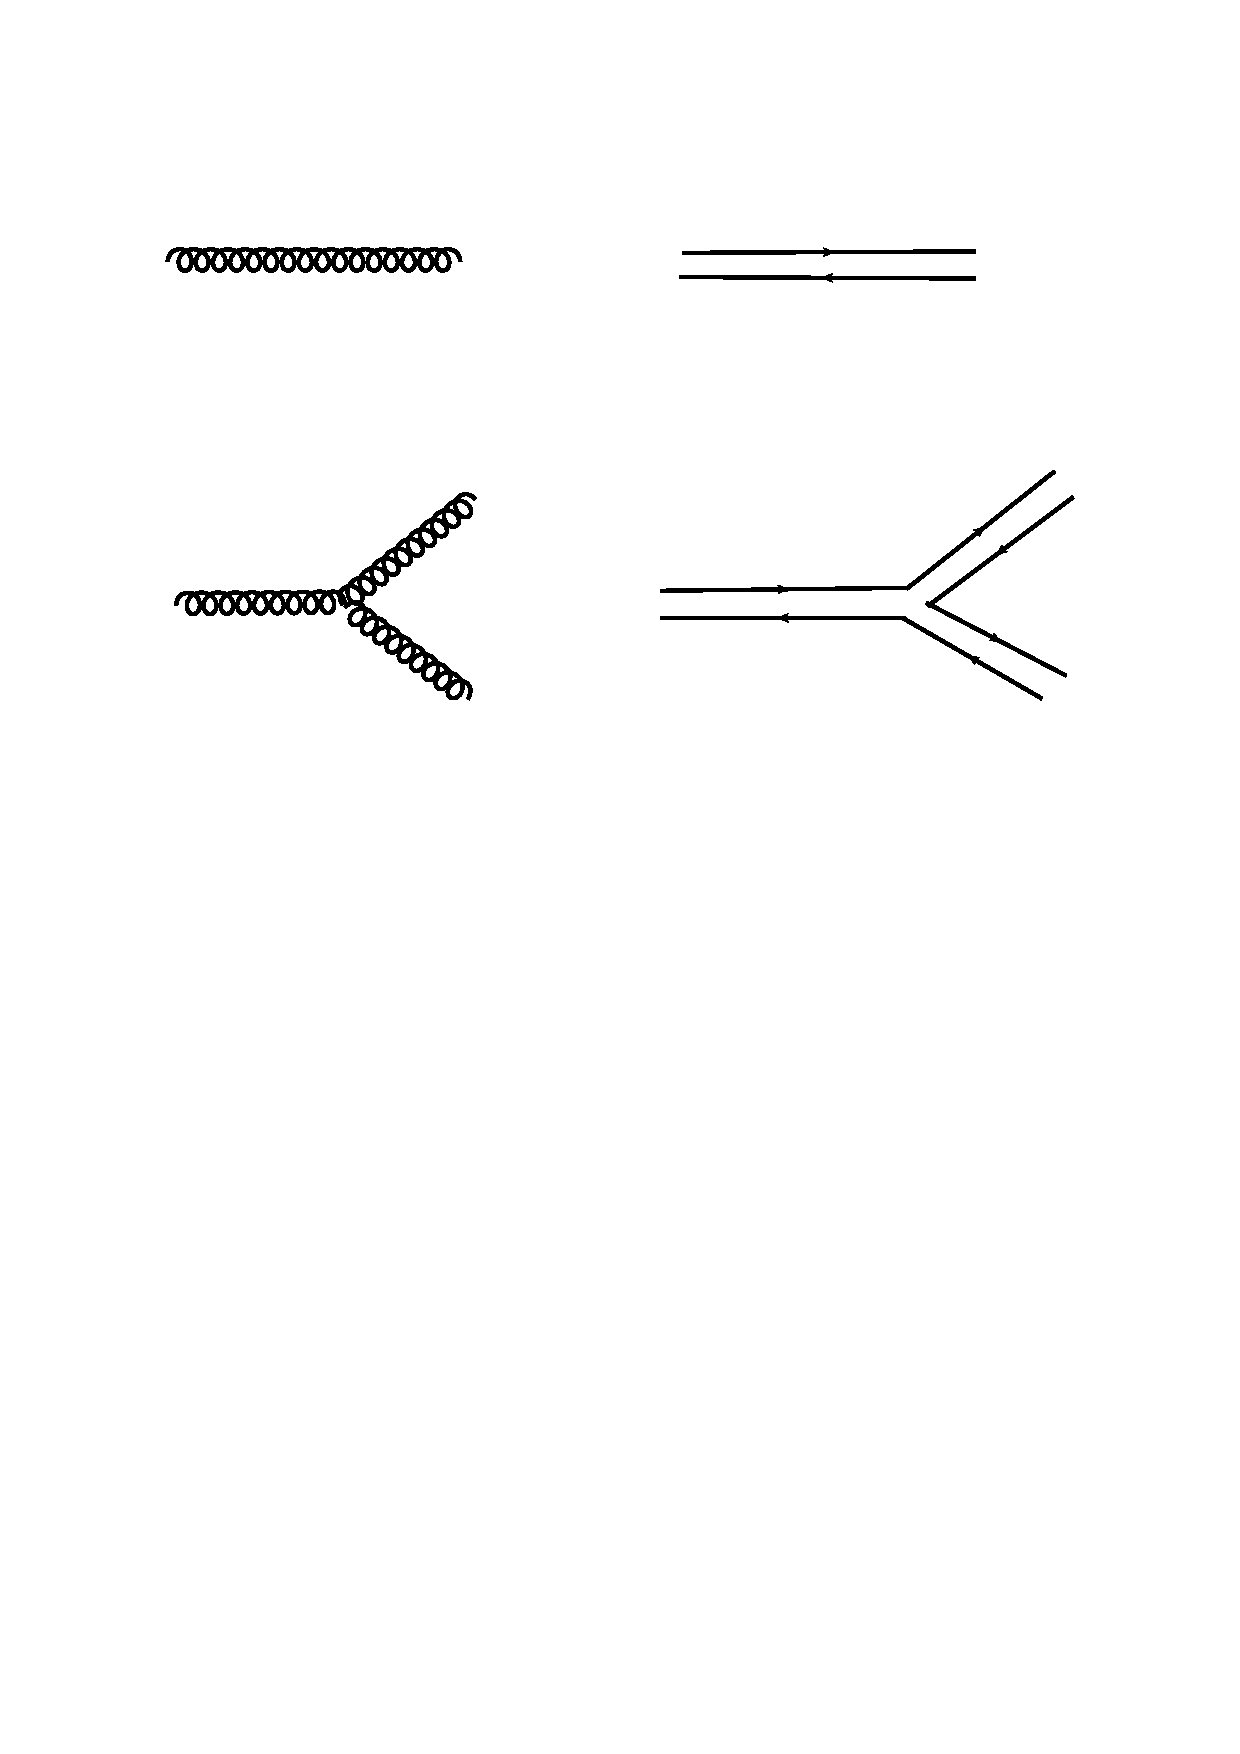
\includegraphics[width=0.35\textwidth]{./Figures/DL1}\end{center}
\end{figure}

\begin{figure}
\begin{center}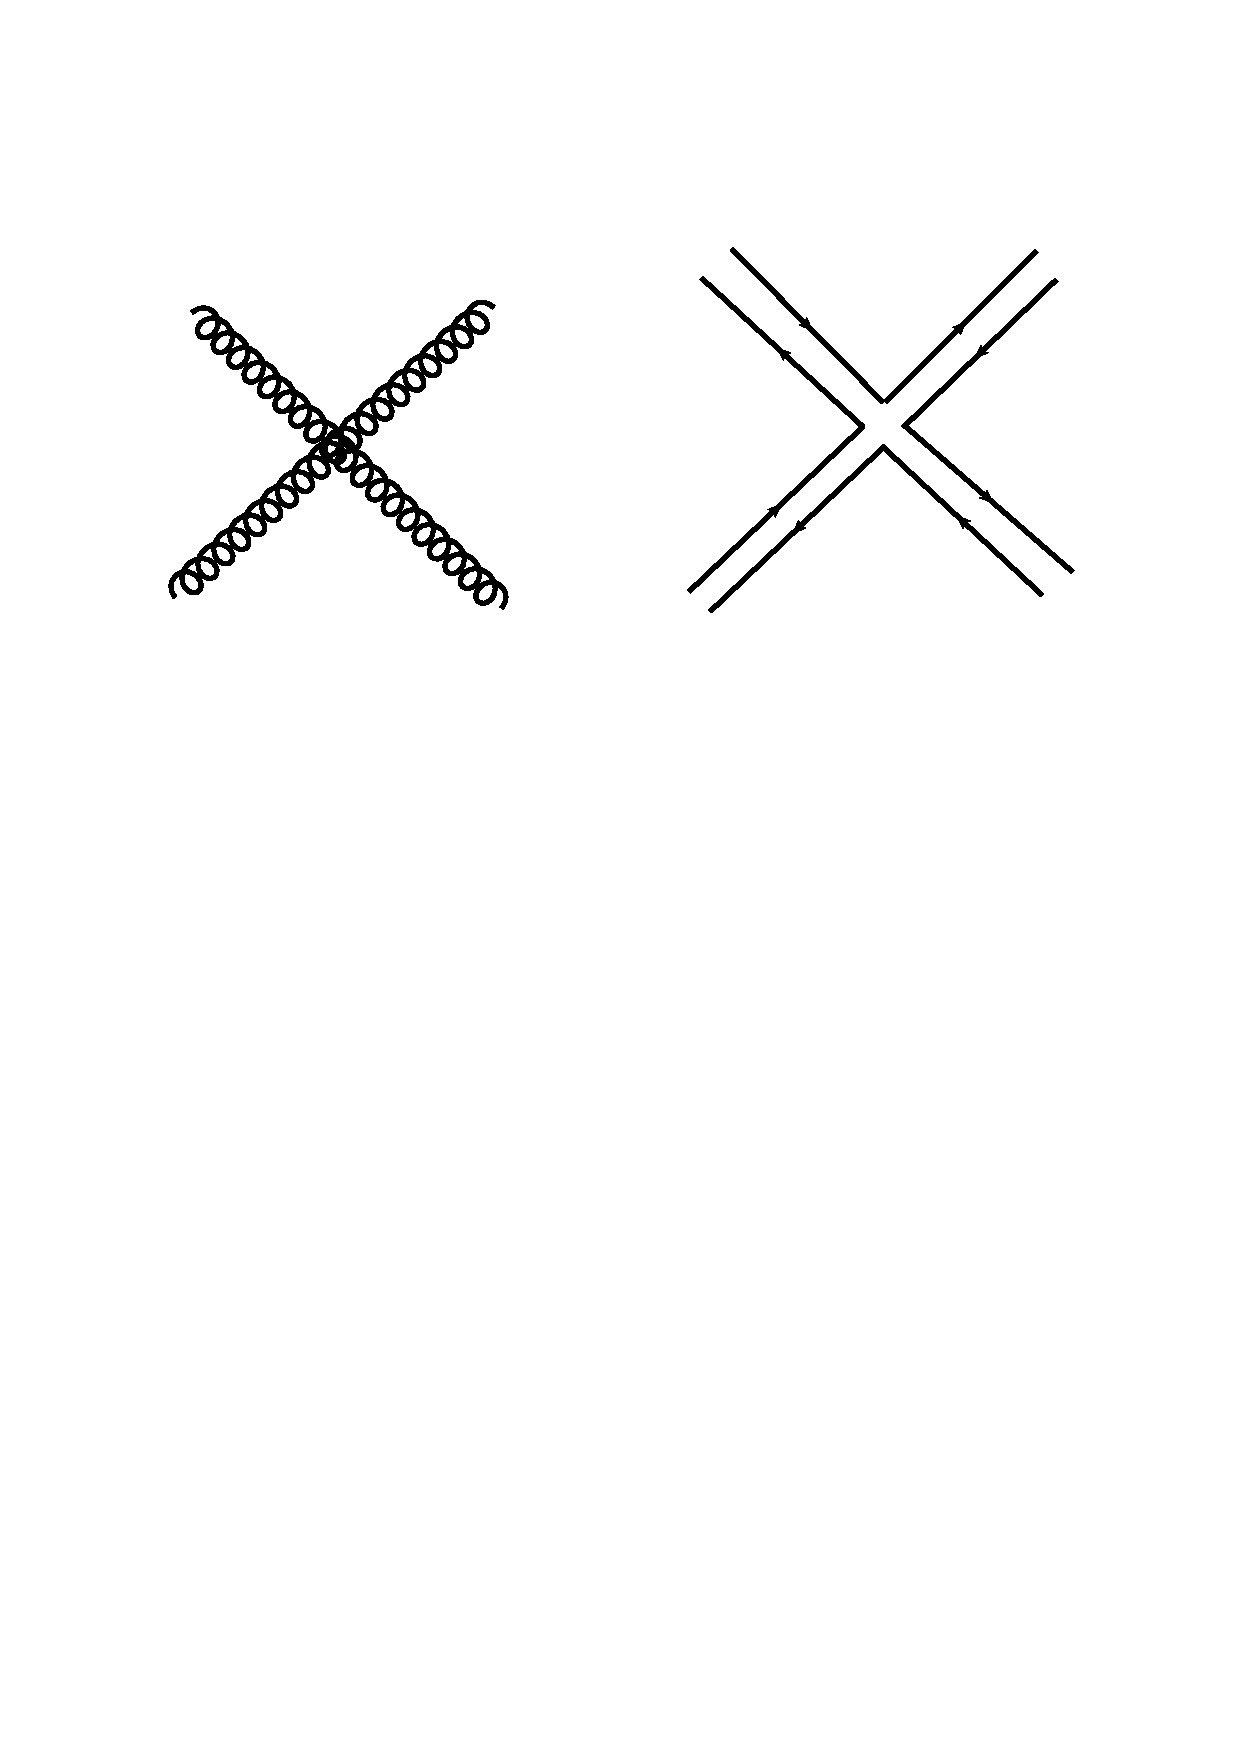
\includegraphics[width=0.35\textwidth]{./Figures/DL3}\end{center}
\caption{\label{fig:dl2}All the diagrams above contribute $\sim N/\lambda$.}
\end{figure}

With our current normalization 
\footnote{We should be careful about field normalizations when doing large N counting for correlation functions. } 
the propagator $\langle \Phi \Phi \rangle$ goes like $\lambda/N$. The propagator in the 
double line notation appears in Fig.(\ref{fig:dl2}). 
We can naively see that the gluon propagator and quark propagator $ \sim 1/N$ 
whereas, the vertex $ \sim N$ in the 't~Hooft limit. 
We can write the gluon propagator as (shown in Fig.(\ref{fig:dl2})), 
\begin{equation}
\label{eq:gluon}
A^{a}_{\mu b}(x) A^{c}_{\nu d}(y) = \left ( \delta^{a}_{d}\delta^{c}_{b} - \frac{1}{N} \delta^{a}_{b}\delta^{c}_{d}\right)
\mathscr{D}_{\mu\nu}(x-y) , 
\end{equation}
In some sense, the gauge field is represented by a ~`quark' with index $i$, and an ~`antiquark' with index $j$. 
The second term in the parentheses is because we need to make the gluon field traceless for the SU($N$) group we are
considering. It would not be present if we were working with U($N$). In any case, in the large $N$, 
the distinction is unimportant. Following the gluon line indices we see, the index pair at the beginning is 
the same as that at the end. In some sense, 
a gluon propagates like quark--anti-quark pair. This observation was made by 't~Hooft when he devised the double-line 
notation. Loosely speaking, we will draw as many lines in a propagator as the indices it carries. Therefore, quark propagator 
is denoted by a single line since it carries one index, whereas a gluon propagator is drawn using double lines, see Fig.(\ref{fig:dl2})
For SO($N$) or USp($N$) theories, the adjoint representation may be written as a product of two fundamental representations 
rather than a product of a fundamental and an anti-fundamental representation (like done for SU($N$) and U($N$)). Since the
fundamental representation is real, there are no arrows on the propagators \footnote{Recall that arrows fix the orientation of complex fields}. Generally, a vacuum diagram has the following dependence on $g_{\text{YM}}$ and $N$, 

\[  \text{Amplitude} \sim \text{diagram} \sim (g_{\text{YM}})^{E} (g_{\text{YM}})^{-V} N^{F} \] 
where E is the number of propagators, V is the number of vertices, F is the number of faces. This has no sensible
$N \to \infty$ limit, since there is no upper limit on F. However, 't~Hooft suggested that we can
take the limit $N \to \infty$ and $g_{\text{YM}} \to 0$ but keep $\lambda = g_{\text{YM}}^{2} N $ remains fixed. 
\[ \text{diagram}(V,E,F) \sim N^{V-E+F} \lambda^{E-V}  \sim N^{\chi} \lambda^{E-V} \] 
where $\chi = F + V - E$ is assured by a theorem due to Euler which we note below.  

\emph{Theorem}: Given a surface composed of polygons with F faces, E edges and V vertices, the Euler character satisfy
$\chi = F + V - E = 2 - 2h$. 
Here, $h$ is the number of handles (also known as `genus' ) of the surface.
Since, in the large $N$ limit, the diagrams with $h = 0$ contribute most 
the large $N$ limit is also known as the planar limit (because $h=0$ means no handles like spheres). Since each Feynman 
diagram can be considered as a partition of the surface separating it into polygons, then the
above theorem also works for our counting in $N$. Only planar diagrams survive in the large $N$ limit.  
As an example, let's consider the diagram shown in Fig (\ref{fig:dia1}), which has four 3-point vertices, six propagators, and four index (color) loops. At this point, we can make some remarks. 1)  The sphere (or the plane) has the largest 
Euler characteristic, $\chi = 2$. 
%The planar diagrams can be drawn on a plane (without crossing) and are also called non-crossing diagrams, 
2) In QED, the expansion parameter is $e^2/4\pi$ = 
1/137 which implies that $e = 0.3$. But in fact, the true expansion parameter in QED is actually  $e^2/4\pi^2$. It is a little gloomy 
for Yang-Mills since there is no
extra $1/4\pi$ and the expansion parameter is $1/N$ or $1/N^2$. This argument is initially due to Witten and can be found in 
\cite{SCA}. 

\begin{figure}
 \label{fig:dia1}
\begin{center}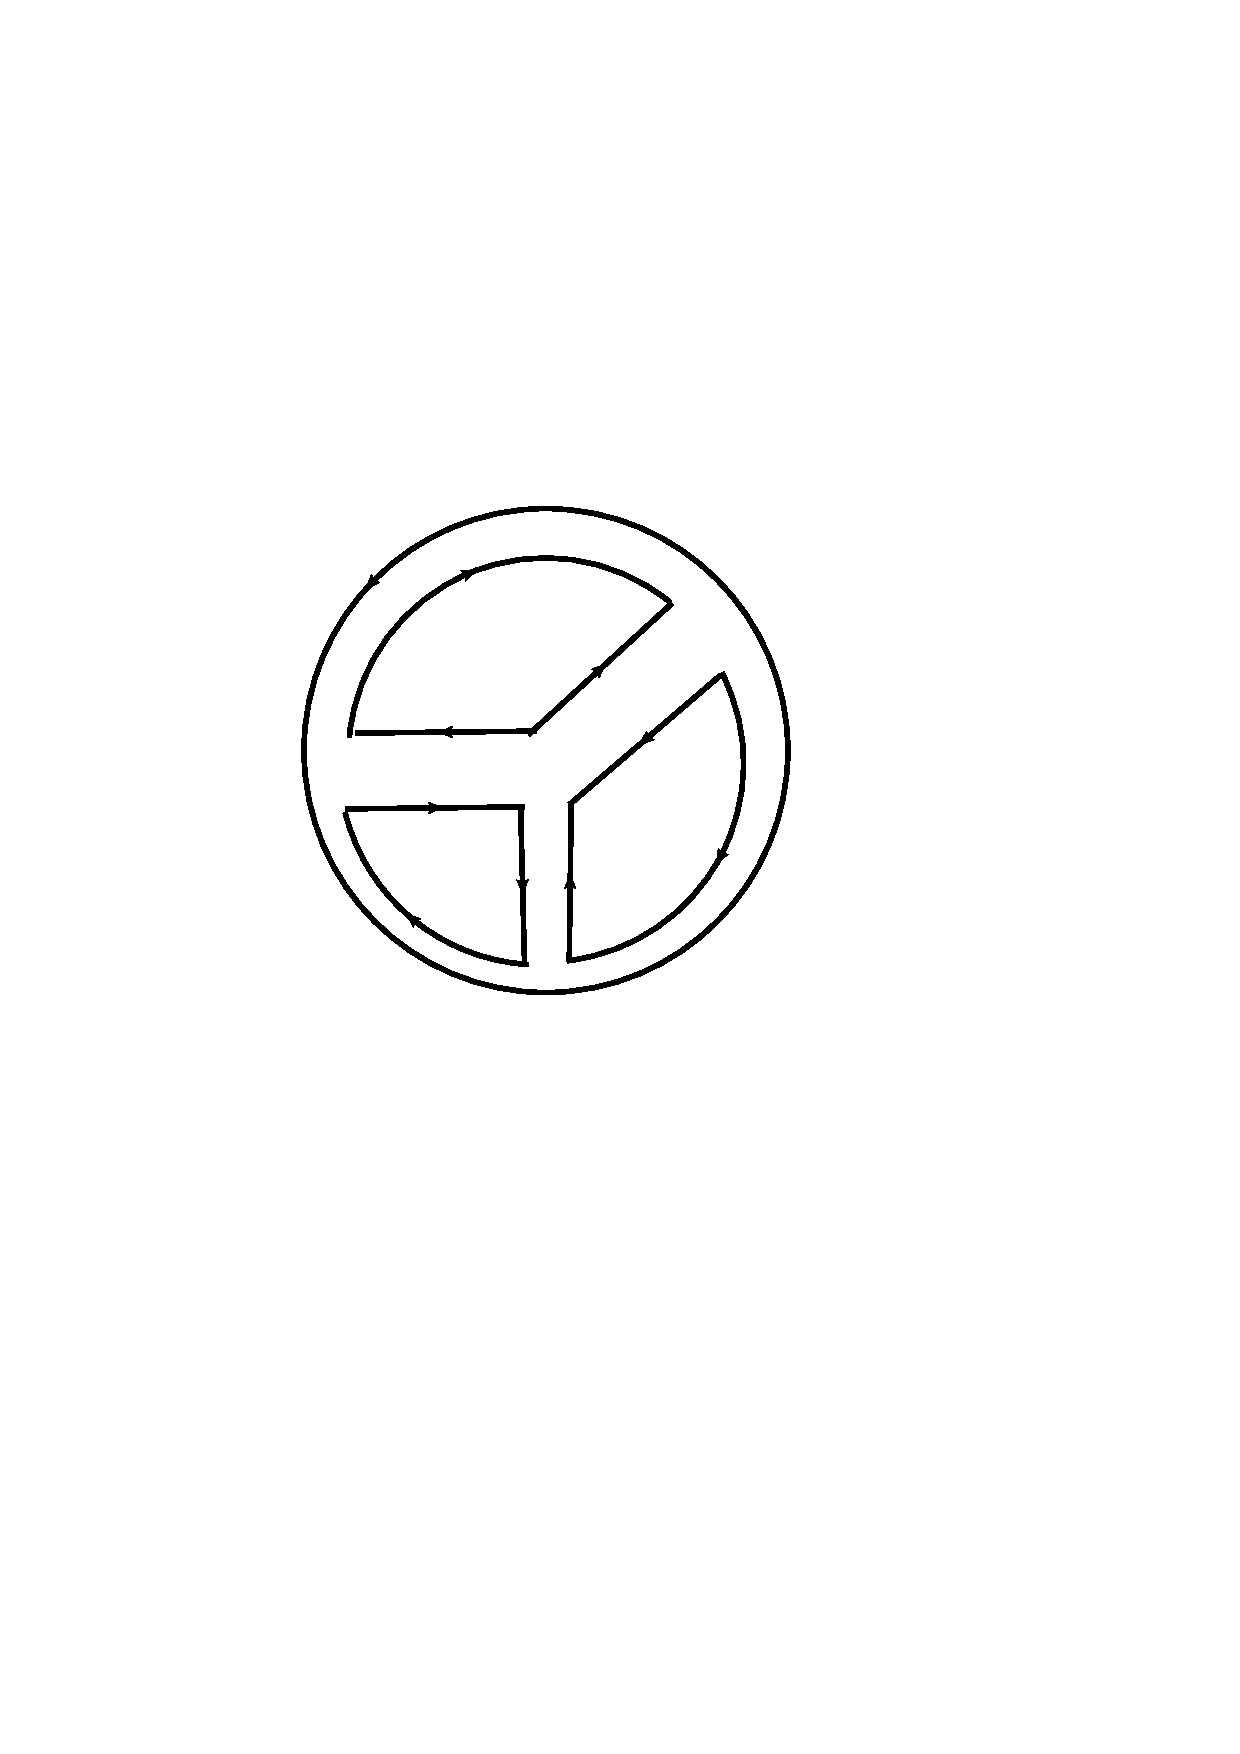
\includegraphics[width=0.25\textwidth]{./Figures/DL5}\end{center}
\caption{\label{fig:dia1}This diagram contributes $\sim N^2 \lambda^2$.}
\end{figure}

\begin{figure}
\begin{center}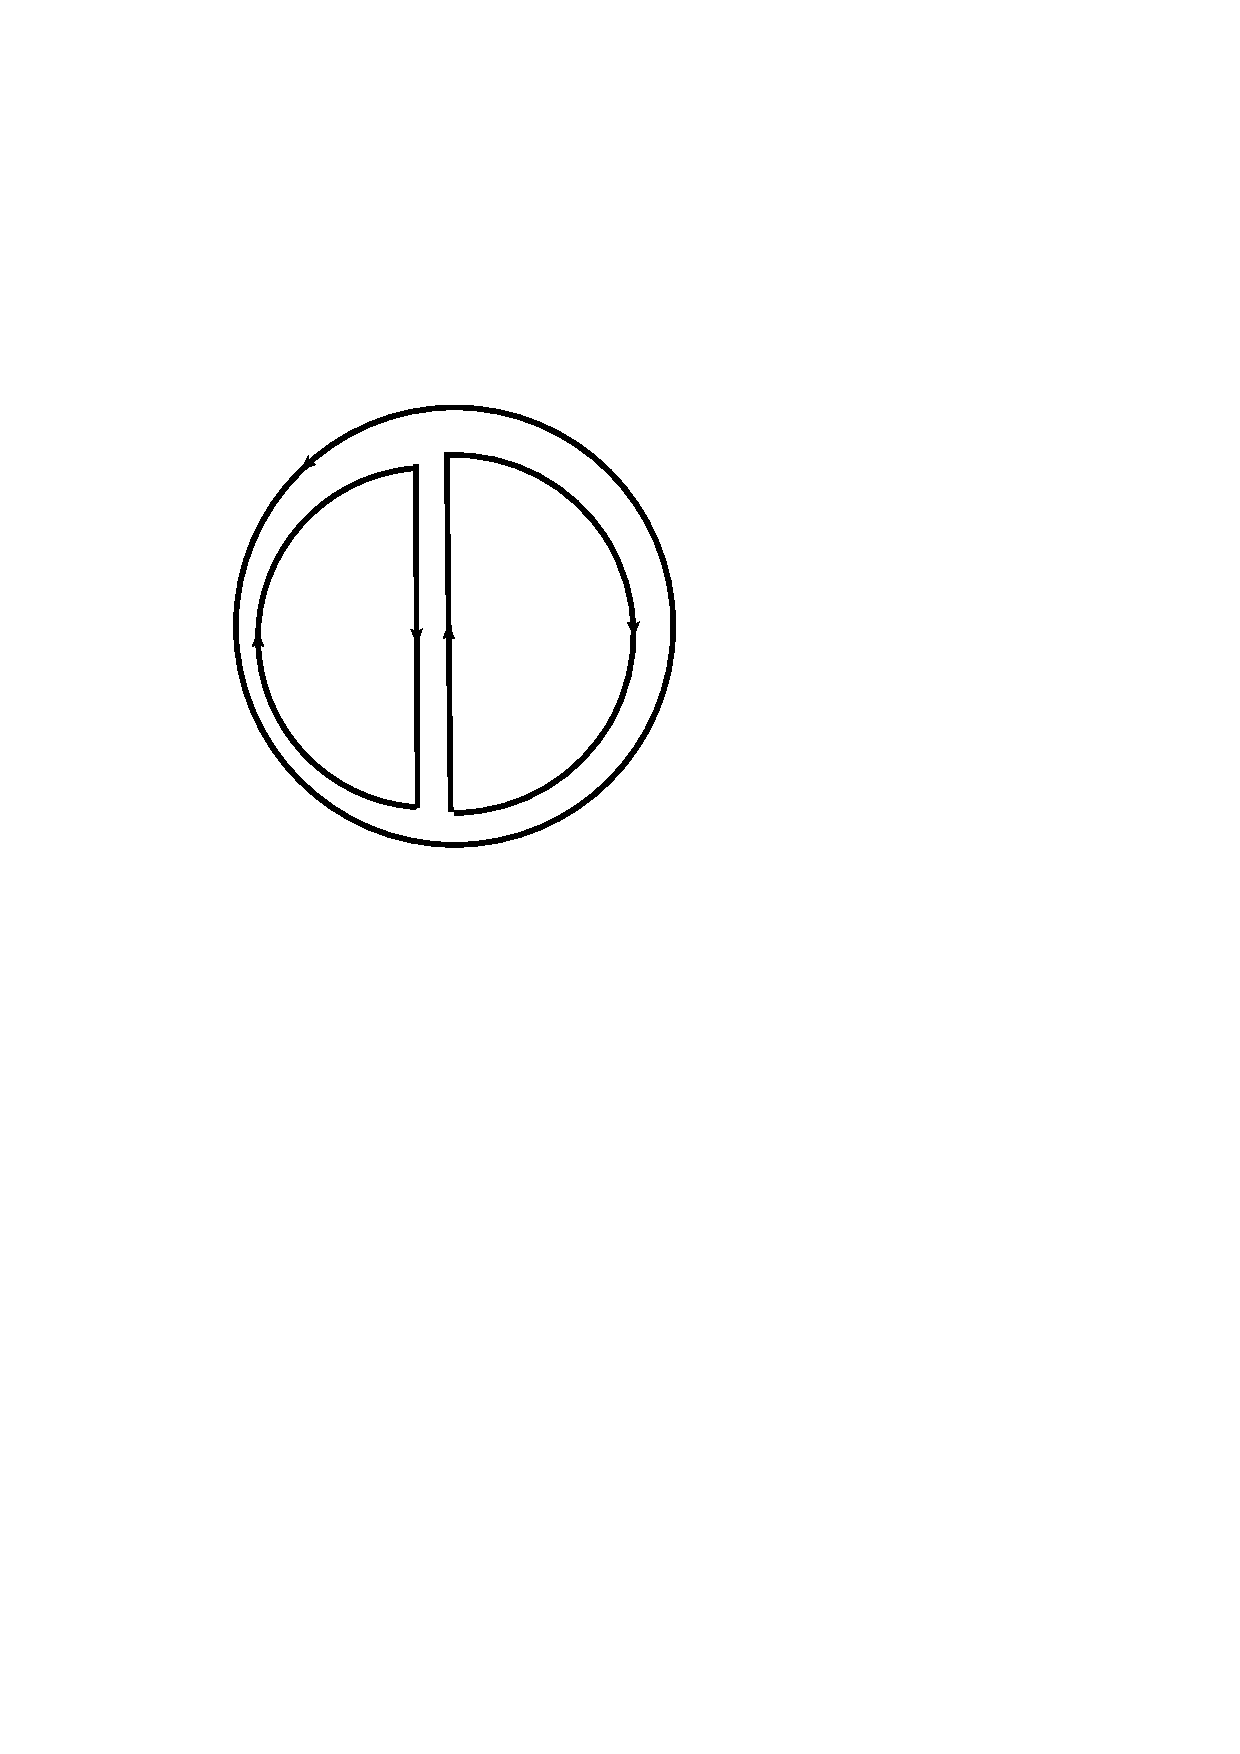
\includegraphics[width=0.25\textwidth]{./Figures/DL4}\end{center}
\caption{\label{fig:dl99}The diagram has $E=3$, $V=2$ and $F=3$ and contributes $\sim N^2 \lambda $.}
\end{figure}
The free energy can be expressed as, 
\begin{align}
  \label{eq:logZ}
   \text{log} \mathscr{Z} =&\sum_{h=0}^{\infty} N^{2-2h} f_{h}(\lambda) \\ 
   				    =& N^{2} f_{0}(\lambda) + f_{1}(\lambda) + \frac{1}{N^2} f_{2}(\lambda) + \cdots
\end{align}
The first term comes from the planar diagrams, the second term from the genus-1 diagrams, and so on.
Hence, in the large $N$ limit, the free energy goes as $\mathscr{O}(N^2)$. 
One might think that the free energy diverges in the large $N$ limit, but we actually calculate, 
\[ \displaystyle\lim_{N \to \infty} \frac{F}{N^2} = \cdots  \] 
which has a sensible large $N$ limit. 

\subsection{Factorization and master field in the planar limit}
General observables we consider are correlation functions of gauge invariant operators, 
\beq
 \label{eq:gsop}
\langle \mathcal{O}_{1}(x_{1}) \mathcal{O}_{2}(x_{2}) \cdots \mathcal{O}_{n}(x_{n})\rangle_{\text{con}}
\eeq 
we will assume that $\mathcal{O}$ is a single trace operator. It is enough to just consider 
them since the multiple trace operator are just products of them. 
\begin{itemize}
\item Single-trace operators : $\mathrm{Tr}(F_{\mu\nu}F^{\mu\nu}) , \mathrm{Tr}(\Phi^n)$ 
\item Double-trace operators : $\mathrm{Tr}(F_{\mu\nu}F^{\mu\nu})\mathrm{Tr}(\Phi^2)$ 
\end{itemize}
Generally, single trace operators take the form, 
\begin{equation}
 \mathcal{O}(x)  = \mathrm{Tr} (\Phi_{1}(x) \cdots \Phi_{k}(x)) 
 \end{equation}
An important thing is to understand how does (\ref{eq:gsop}) behaves in the large $N$ limit. 
Consider the following, 


\beq
 \label{eq:trick1}
 \mathscr{Z}[J_{1}, \cdots J_{n}] = \int \mathcal{D}A \mathcal{D}\Phi \cdots \exp \left [ S_{0} + 
 N \sum_{j} \int J_{i}(x)\mathcal{O}_{i}(x) \right] 
\eeq 
Then, (\ref{eq:gsop}) can be written as, 
\beq
 \label{eq:trick2}
\langle \mathcal{O}_{1}(x_{1}) \mathcal{O}_{2}(x_{2}) \cdots \mathcal{O}_{n}(x_{n})\rangle_{\text{con}} = 
\displaystyle\lim_{\text{all} ~ J \to 0} \frac{\delta^{n} \text{log} \mathscr{Z}}{\delta J_{1}(x_{1}) 
\cdots \delta J_{n}(x_{n}) } \frac{1}{N^n}
\eeq 
But, we know that 
\beq
\text{log} \mathscr{Z}[J_{1} \cdots J_{n}] = \sum_{h=0}^{\infty} N^{2-2h} f_{h}(\lambda, \cdots)
\eeq
So, we get, 
\beq
 \label{eq:trick3}
\langle \mathcal{O}_{1}(x_{1}) \mathcal{O}_{2}(x_{2}) \cdots \mathcal{O}_{n}(x_{n})\rangle_{\text{con}} 
\sim N^{2-n} \left [ 1 + \mathscr{O}(\frac{1}{N^2}) \right] 
\eeq 
and it is equivalent to,  
\[ \langle I \rangle \sim \mathscr{O}(N^{2}) + \mathscr{O}(N^{0}) \] 
\[ \langle \mathcal{O} \rangle \sim \mathscr{O}(N) + \mathscr{O}(N^{-1}) \] 
\[ \langle \mathcal{O}_{1}\mathcal{O}_{2}\rangle_{\text{con}} \sim \mathscr{O}(N^{0}) + \mathscr{O}(N^{-2}) \] 
\[ \langle \mathcal{O}_{1}\mathcal{O}_{2}\mathcal{O}_{3} \rangle_{\text{con}} \sim 
\mathscr{O}(N^{-1}) + \mathscr{O}(N^{-3}) \] 


This implies that for two gauge-invariant operators, A and B (in the large $N$ limit) 
\[ \langle AB \rangle \sim \langle A \rangle  \langle B \rangle + \mathscr{O}(\frac{1}{N^2}) \] 
The variance of operators vanish in this limit and there are no fluctuations. All this has been done for 
the case of pure gauge theory but this can be extended to fermions as well. To summarize, - the average 
value is the only calculated value via the master field, which we will now discuss. 
Another immediate consequence of this can be applied to the Wilson loop as done by Migdal and Makeenko 
\cite{Makeenko:1979pb}. We can show that the following has, 
a decoupling property in the large $N$ limit, 

\beq
 \label{eq:migdal1}
\langle \phi(\mathcal{C}_{1})~ \phi(\mathcal{C}_{2})\rangle \to \langle 
\phi(\mathcal{C}_{1})\rangle \langle \phi(\mathcal{C}_{2})\rangle
\eeq

The above equation \ref{eq:migdal1} implies that $ \phi(\mathcal{C})$ can be considered 
as a classical field in loop space, 
but it does not imply that the gauge field, $A_{\mu}$ become classical in this limit. 
As it has been discussed above, in the large $N$ limit the path-integral is peaked 
around a particular configuration. 
This is tied to the idea of a master field (coined by Coleman) initially due to Witten. 
In this limit, the probability of finding 
any gauge-invariant 
quantity away from its expectation value goes to zero as $N \to \infty$ 
\cite{Gopakumar:1994iq}.
The best way to think of the master field is to draw an analogy 
with the path-integral approach. 
It tells us that Green's functions for a quantum theory are obtained 
by summing over all possible classical motions. 
In the limit that $\hbar \to 0$, the measure in the functional space 
becomes sharply concentrated about the solution to
 the classical equations of motion, in the limit of vanishing $\hbar$, 
all quantities are given by their value evaluated at the classical solution. 
In the case of the large $N$ limit of a gauge theory, there exists a 
master field configuration. 
All gauge-invariant operators expectation value can be evaluated using this master field. 
In case of large $N$ QCD, the master field(s) are four $N \times N, 
M_{i}$ matrices, where $N \to \infty$.  
Some observations are in order now,  

\begin{itemize}
\item We can calculate all the correlation functions of the invariant 
observables simply by taking the trace of the product of master fields and not doing any integrals. 
\item The master field is not unique since we are interested only in 
gauge-invariant quantities, any gauge transform of a master field is also a master field. 
So more precisely, one should talk about ~`master orbit of the gauge 
group'. 
\item For the classical analogy, we have a well-defined method of 
finding the single field configuration, i.e by solving classical equations of motion. 
But finding the master field is not a panacea, since one does not have a well-defined prescription yet.
\end{itemize}   


\section{Toward the AdS/CFT correspondence} 
The study of non-perturbative formulations of superstring theories is 
greatly facilitated by the idea of the AdS/CFT correspondence. AdS/CFT is 
a strong/weak duality between two theories (one with gravity and the other without) 
first proposed by Maldacena in 1997. It is inspired by the structure and symmetries of the 
space-time and the conformal field theory (CFT). 
This conjecture is again an example of how interesting the large 
$N$ limit of gauge theories can be and since we have already discussed 
that in the previous section, we can start to formally discuss 
the holographic conjecture (or AdS/CFT correspondence). 
We will first review some concepts required from String theory for stating this conjecture 
and then discuss the decoupling limit which is central to the idea of this 
correspondence. We will then formally define this conjecture in \ref{sec-ads}.  

\subsection{D$p$-branes, and black $p$-branes} 

The low-energy limit ($l_{s} \to 0$) of string theory describes classical gravity (called ~`supergravity'). 
The black $p$-branes are solutions of supergravity. at non-zero temperature. They can also be thought of as black holes that 
extend in $p$ spatial dimensions. 
$\textit{Dp-branes}$ are extended objected in (p+1) dimensions. 
They have their own identity in string theory and are the central motivation for AdS/CFT correspondence. 
A D$p$-brane is defined as a hypersurface where open strings can end with 
Dirichlet boundary conditions (endpoints fixed). 
The open-string picture of D-brane describes a p+1 dimensional SYM. 
D3-brane is special because the world volume is four-dimensional 
and that is where the SYM gauge theory lives. The closed-string picture of 
D-branes relies on the fact that the closed strings do not have to 
be attached to the D-branes. They can propagate freely in directions orthogonal to the brane and live in extra dimensions. 
It is also important to note here that D-branes break half of the supersymmetry and are BPS states. 
The same use of $p$ for both black $p$-branes and $\textit{D$p$-branes}$ is 
confusing. However, Polchinski \cite{Polchinski:1995mt} realized that stack of D$p$-branes 
and extremal black $p$-branes are the same objects.
As mentioned before, D-branes give rise to gauge theories. The open 
string states are described with a $N \times N$ matrix. 
In the low energy approximation, this gives rise to supersymmetric 
Yang-Mills theory. The gauge theory is controlled by two parameters, 
$\lambda, N$, whereas, in the supergravity, we have the string length, $l_{s}$ and the string coupling, $g_{s}$. 

In general, the superstring theory contains both closed and open strings. 
The former mediates the gravitational force, and the latter mediates the gauge interactions. 
Open strings can end in objects which are called $\textit{D-branes}$. 
While the closed string can propagate anywhere in the bulk (1+9)-dimensional spacetime, 
the endpoints of an open string must be attached to the $\textit{D-branes}$.  
As a particular case of these $\textit{D-branes }$, we have $\textit{D-particles}$, 
which look like pointlike objects. In the low-energy limit, the strings can be
 viewed as particles. We can express the black hole as a combination of 
 $N$ $\textit{D-particles}$, 
where $N$, the number of $\textit{D-particles}$ is large and it implies that 
the geometry is weakly curved and the size of the black hole is large. Quantum gravity effects become
large when $N$ is small. 

\subsection{The decoupling limit} 

The limit in which the conjecture holds can be argued as follows. 
Consider the gauge theory in four dimensions which are associated 
with the world-volume of D3 branes. 
The action for string theory with $D3$-branes 
can be written as, 
\begin{equation}
S = S_{\text{bulk}} + S_{\text{brane}}  + S_{\text{interaction}} 
\end{equation}
where $ S_{\text{bulk}}$ is the action of closed strings in the bulk (some six-dimensional space), 
$S_{\text{brane}}$ is the action due to open strings attached to 
$D3$-branes. The third term is just the interaction term between
the open and closed string pieces. It is worthwhile to note that 
$S_{\text{interaction}} \approx g_{s} l_{s}^4$, and vanishes
in the low-energy approximation. In such a situation, the entire 
action is factored into bulk and brane parts. 
The bulk parts represent the SUGRA and the brane then represents 
$\mathcal{N}=4$ SYM. 
This is only one half of the story. Another half can be seen by 
looking at the extremal $p$-brane 
and noting that the low-energy limit is similar to taking the 
near-horizon limit and in that case the 
factorization gives us like before SUGRA in the bulk
but the other part gives the AdS$_5 \times S_5$.
Therefore, in the large $N$ limit, $\mathcal{N}=4$ SYM on $\mathbb{R}^{3,1}$ is dual to 
Type IIB SUGRA on AdS$_5 \times S_5$.
The decoupling limit and the complete steps leading to the 
correspondence are shown in Fig.(\ref{fig:AdS1}). 

\begin{figure}[h!]
\label{fig:AdS1} 
  \centering
      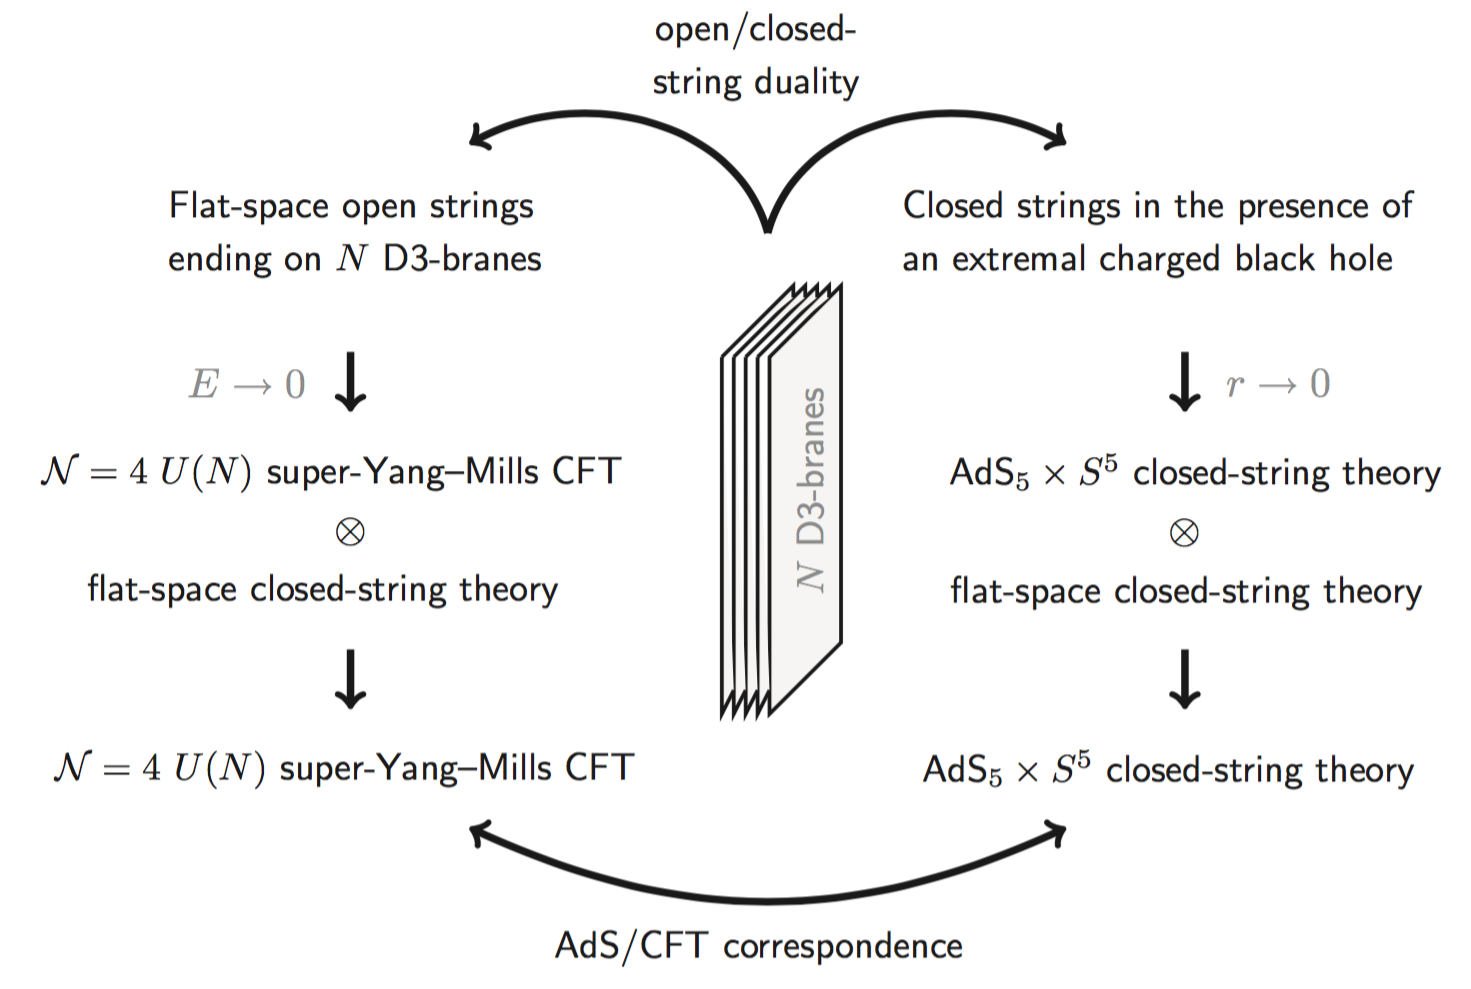
\includegraphics[width=0.9\textwidth]{./Figures/ads22.jpg}
  \caption{\label{fig:AdS1}Diagrammatic representation of the AdS/CFT duality. Picture from \cite{ZEA}.}
\end{figure}



\subsection{Symmetries, degrees of freedom, and holographic dictionary} 

AdS/CFT correspondence can also be loosely suggested based on the following observation. First note that 
the line element of the AdS space  in $(d+1)$-dimensions is given by,
\beq
ds^2\,=\,{L^2\over z^2}\,(-dt^2+d\vec x^2+dz^2)\,\,,
\label{AdS_metric}
\eeq
The constant $L$ is a global factor in (\ref{AdS_metric}), which we will refer 
to as the anti-de Sitter radius. 
The (conformal) boundary of the AdS space is located at $z=0$. Notice that the metric (\ref{AdS_metric}) is singular at $z=0$.
This means that we will have to introduce a regularization procedure in order to define quantities in the AdS boundary.
The isometries of (d+1)-dimensional anti-de Sitter space is $SO(d,2)$ symmetry which is the same 
as the conformal symmetry of $d$-dimensional space-time. In addition, we have the isometries of $S^{5}$ 
which form SU(4), which is $\approx$ SO(6). This group is the same as the R-symmetry of the $\mathcal{N}$ = 4 SYM theory. 
The full isometry supergroup of the $AdS^{5}$ $\times$ $S^{5}$ background is $SU(2, 2|4)$, 
which is identical to the $\mathcal{N}$ = 4 superconformal symmetry.

Firstly, we will discuss the QFT side. To regulate the theory we put both a UV and IR regulator. We place the system in a spatial 
box of size $R$ (which serves as an IR cutoff)  and we introduce a lattice spacing $\epsilon$ that acts as a UV regulator. In $d$ 
spacetime dimensions the system has $R^{d-1}/\epsilon^{d-1}$ cells. Let $c_{QFT}$ be the number of degrees of freedom per 
lattice site, which we will refer to as the central charge. Then, the total number of degrees of freedom of the QFT is:
\beq
N_{dof}^{QFT}= \Big({R\over \epsilon}\Big)^{d-1}\,\,c_{QFT}\,\,.
\eeq
The central charge is one of the main quantities that characterize a CFT. If the CFT is  a 
$SU(N)$ gauge field theory,  such as the theory with four supersymmetries which will be described below, the fields are $N\times N$ 
matrices in the adjoint representation which, for large $N$, contain $N^2$ independent components. Thus, in  these $SU(N)$ CFT's
 the central charge scales as  $c_{SU(N)}\sim N^2$. Central charges scale as the number of generators of a group when N is large. 
We can then compute the number of degrees of freedom of the $AdS_{d+1}$ solution. According to the holographic principle and to the 
Bekenstein-Hawking formula, the number of degrees of freedom contained in a certain region is equal to the maximum entropy and is given by
\beq
N_{dof}^{AdS}={A_{\partial}\over 4 G_N}\,\,,
\eeq
with $A_{\partial}$ being the area of the region at boundary $z\to 0$ of  $AdS_{d+1}$. Let us evaluate $A_{\partial}$ by integrating
 the volume element corresponding to the metric (\ref{AdS_metric}) at a slice $z=\epsilon\to 0$:
\beq
A_{\partial}\,=\,\int_{{\mathbb R}^{d-1},\, z=\epsilon}\,
 d^{d-1}\,x\,\sqrt{g}\,=\,\Big({L\over \epsilon}\Big)^{d-1}\,\
 \int_{{\mathbb R}^{d-1}}\, d^{d-1}\,x\,\,.
 \label{A_delta_unregularized}
 \eeq
The integral on the right-hand-side of (\ref{A_delta_unregularized}) is the
the volume of ${\mathbb R}^{d-1}$, which  is infinite. As we did on the QFT side, we regulate it 
by putting the system in  a box of size $R$:
\beq
\int_{{\mathbb R}^{d-1}}\, d^{d-1}\,x=R^{d-1}\,\,.
\eeq
Thus, the area of the $A_{\partial}$ is given by:
\beq
A_{\partial}\,=\,\Big({RL\over \epsilon}\Big)^{d-1}\,\,.
\eeq
Let us next  introduce the Planck length $l_P$ and the Planck mass $M_P$ for a gravity theory in $d+1$ dimensions  as:
\beq
G_N\,=\,(l_P)^{d-1}\,=\,{1\over (M_P)^{d-1}}\,\,.
\label{Planck_l_M}
\eeq
Then, the number of degrees of freedom of the $AdS_{d+1}$ space is:
\beq
N_{dof}^{AdS}={1\over 4}\, \Big({R\over \epsilon}\Big)^{d-1}\,
 \Big({L\over l_P}\Big)^{d-1}\,\,.
\eeq
By comparing $N_{dof}^{QFT}$ and $N_{dof}^{AdS}$  we conclude that they scale in the same way with the IR and UV cutoffs  $R$ and $\epsilon$ and we can identify:
\beq
{1\over 4}\,\,\, \Big({L\over l_P}\Big)^{d-1}\,=\,  c_{QFT}\,\,.
\label{holo_centralCharge}
 \eeq
The action of our gravity theory in the $AdS_{d+1}$ space of radius $L$ contains a factor $ L^{d-1}/G_N$. 
Thus, taking into account the definition of the Planck length in (\ref{Planck_l_M}), we conclude that the classical  gravity theory is reliable if:
\beq
{\rm classical\,\, gravity\,\, in\,\, AdS}\to \Big({L\over l_P}\Big)^{d-1} \gg 1\,\,,
\eeq
which happens when the AdS radius is large in Planck units. Since the scalar curvature 
goes like $1/L^2$, the curvature
is small in Planck units. Thus, a QFT has a ~`classical gravity' dual when $c_{QFT}$ is 
large, or equivalently if there is a large number of degrees of freedom per unit volume or a large number 
of species (which corresponds to large $N$ limit for $SU(N)$ gauge theories). 

\section{\label{sec-ads}AdS/CFT and holographic dualities for lower 
dimensional SYM theories}

The AdS/CFT correspondence (also gauge/gravity duality) is a conjecture which relates
the string theory or M-theory on a background of the form 
AdS$_{5} \times S_{5} $, where $S_{5}$ is a compactified manifold 
(called five-sphere), to a 
conformally invariant supersymmetric quantum field theory 
in four space-time dimensions, which is, in fact, the boundary 
of the AdS$_{5}$. Soon after this conjecture, the authors of 
\cite{Gubser:1998bc,Witten:1998qj} proposed concrete relations 
between the gauge and gravity theories which are now known as 
GKPW or GKP-W relations. 
A concrete possibility of holography in quantum gravity was in 
fact proposed several years before the 
AdS/CFT conjecture by 't~Hooft in \cite{tHooft:1993dmi} and then 
subsequently by Susskind 
in \cite{Susskind:1994vu}. In Table (\ref{tab:dic1}), 
we present a mapping between the bulk and boundary
theories. 

\vspace{4mm} 

\begin {table}[htbp] 
\begin{center}
\begin{tabular}{ |  p{5cm} |  p{8cm} |}
    \hline
    \emph{Boundary: Gauge theory}  & \emph{Bulk: Gravity }   \\ \hline \hline 
     Partition function   &  Partition function  ($Z_{\text{CFT}} = Z_{\text{gravity}}$) \\ \hline 
     Wilson loop along $\mathcal{C}$ & String worldsheet with end points on $\mathcal{C}$  \\ \hline 
     Deconfinement transition & Transition between black hole solutions based on entropy competition \\ \hline
     Number of degrees of freedom & Radius of AdS space  \\ \hline
     Free energy & On-shell value of the action  \\ \hline
\end{tabular}
\vspace{3mm}
\caption {\label{tab:dic1}The basic mapping in AdS/CFT correspondence.} 
\end{center}
\end {table}

We now move to general dualities relating $p+1$-dimensional SYM theory to the world volume of D$p$-branes
(in some limit). Let us consider $N$-parallel D$p$-branes separated by some distances which we 
refer by $r$. At low energies, the theory on the D$p$ brane decouples from the bulk. It is more convenient to
take the energies fixed and take, 
\[ \alpha^{\prime} \rightarrow 0  \hspace{8mm} ; \hspace{8mm} U \equiv \frac{r}{\alpha^{\prime}} = \text{fixed} \hspace{8mm}
; \hspace{8mm} g^{2}_{\text{YM}} = \frac{1}{2\pi} \frac{g_{s}}{\alpha^{\prime}} = \text{fixed}   \]
here, $\alpha^{\prime}$ is the string tension and $g_{s}$ is the string coupling. The 
second condition ensures that the mass of the stretched strings is fixed. This limit is known as ~`decoupling limit'.  
At a given energy scale, U, the effective dimensionless coupling constant in 
the corresponding super Yang-Mills theory is $ g_{\text{eff.}}^{2} \approx g_{\text{YM}}^{2} NU^{p-3}$. 
Therefore, perturbative calculations in super Yang-Mills can be trusted in the region 
\begin{equation}
 g_{\text{eff.}}^{2} \ll 1 \hspace{10mm} \begin{cases}
     U\gg (g^2 N)^{1/(3-p)} ; \hspace{8mm}p<3     \\
    U \ll 1/(g^2 N)^{1/(p-3)} ; \hspace{5mm} p>3  
      \end{cases}
    \end{equation} 
In the large $N$ 't~Hooft limit, the natural coupling becomes $ \lambda = N g_{YM}^{2}$. 
The bosonic part of the action is given as,
\begin{equation}
S_{B} = \frac{N}{\lambda}  \int dt ~ dx^p \mathrm{Tr}\left[  - \frac{1}{4} F_{\mu\nu}^2 - 
\frac{1}{2} D^\mu \Phi^I D_\mu \Phi^I + \frac{1}{4} \left[ \Phi^I , \Phi^J \right]^2  \right]
\end{equation}
and the fermionic action is,
\begin{eqnarray}
\mathcal{S}_{F} = -\frac{1}{2} \frac{N}{\lambda} \int dt ~ dx^p \mathrm{Tr} \overline{\Psi} \left( \gamma^\mu D_\mu - i  \left[ \gamma^I \Phi^I , \cdot \right] \right) \Psi
\end{eqnarray}
where $x^\mu$ with $\mu = 0, \ldots, p$ are the world volume coordinates 
with time $x^0 = t$ and 
spatial coordinates $x^i$ with $i=1,\ldots,p$. Then $\Phi^I$ with $I = 1+p, 
\ldots, 9$ are the spacetime 
scalars representing the transverse degrees of freedom of the branes. 
They are $N \times N$ Hermitian 
matrices transforming in the adjoint representation of the gauge group. 
The fermion $\Psi$ is a $(1+9)$-dimensional 
Majorana-Weyl spinor and also transforms in the adjoint. 
The field strength is defined as usual, $F_{\mu\nu} = \partial_\mu A_\nu - 
\partial_\nu A_\mu + i [ A_\mu , A_\nu ]$, and $D_\mu = \partial_\mu - i [ A_\mu, \cdot]$, with $A_\mu$ 
the gauge field potential transforming in the adjoint. 

The general gauge/gravity duality \cite{Itzhaki:1998dd} 
states that at finite temperatures there is a dual closed IIA ($p$ even) or IIB ($p$ odd)
string theory description of this gauge theory in terms of the decoupling limit of thermal D$p$-branes. 
 In the large $N$ 't~Hooft limit this string theory description may reduce to one in IIA or IIB supergravity. 
In addition, the $(p+1)$-form potential carries the charge of the $N$ D$p$-branes. Here $t$ and $x^i$ 
are the D$p$-brane $(p+1)$-dimensional world volume coordinates. The radial coordinate of the metric 
is identified with an energy scale associated with the expectation value of the scalars in the MSYM. 
It is important to note that, this metric is defined in 9+1 dimensions, as required by superstring theory and 
for $p=3$, the dilaton, or equivalently the string coupling is constant and independent of U.
This is the $p=3$ superconformal case and corresponds to the original conjecture proposed by Maldacena. 
If we impose the decoupling limit to the supergravity metric, we will get the metric of the black $p$-brane. 
The black brane is a classical solution to the supergravity (low energy supersymmetric effective 
description of superstring theory). Additionally, in 
order to trust the supergravity solution, we need the curvature and 
dilaton to be very small, which results in the following inequality, 
\begin{equation}
1 \ll g_{\text{eff.}}^{2} \ll N^{4/(7-p)} 
\end{equation}
We directly see that perturbative super-Yang-Mills and supergravity descriptions do not overlap. 
The radius of curvature $R$ goes as,
$\alpha' /R^2 \sim \left( U / \lambda^{1/(3-p) } \right)^{\frac{3-p}{2} }$. 
We will consider the large $N$ 't~Hooft limit, where it is natural to take,
\begin{eqnarray}
N \to \infty \; , \qquad \frac{U}{\lambda^{1/(3-p)}}  \; , \; \frac{U_0}{\lambda^{1/(3-p)}}  \sim \mathrm{finite}
\end{eqnarray}
and we find that in this large $N$ limit the solution is well described by 
semiclassical string theory since the dilaton will everywhere be small. In order to ensure that supergravity 
gives a good description we shall in addition require that the curvature $\alpha'$ corrections are small, 
and so we must take,
\begin{eqnarray}
U  \; , \; U_0 \ll \lambda^{1/(3-p)} \; .
\end{eqnarray}
We emphasise that we require these quantities to be small, but finite, in the large $N \to \infty$ limit. 

In Chapter \ref{ch3}, we will discuss the large $N$ limit of two-dimensional SYM theory with sixteen supercharges
and show some qualitative agreement with holography. 
The phase diagram of thisYang-Mills theory which is compactified on a torus is labeled by two parameters; 
the extent of the lattice in the Euclidean time direction \& the extent of spatial direction. These two 
directions are distinguished by the boundary conditions on the fermions, which is anti-periodic in the
temporal direction and periodic in the spatial direction.  
$\mathcal{N}$ = (8,8) SYM Euclidean action in two dimensions is given by, 
\begin{eqnarray}
&& 
       S=\frac{N}{\lambda}\int{}{\rm d}^2x\ {\rm tr} 
             \left\{ \frac{1}{4}F^2_{\mu\nu} 
                    + \frac{1}{2}(D_\mu X_i)^2 - \frac{1}{4}[X_i,X_j]^2  
             \right.  \nonumber \\
&& 
      \hspace{3cm} \left.
          +\frac{1}{2} \Psi_\alpha  D_0 \Psi_\alpha 
          -\frac{i}{2} \Psi_\alpha (\gamma_{1})_{\alpha \beta} D_1 \Psi_\beta 
        + \frac{1}{2}\Psi_\alpha (\gamma_i)_{\alpha \beta} [X_i, \Psi_\beta] \right\},
        \label{cont_action}
\end{eqnarray}
where, the Roman indices $i,j$ run from $2$ to $9$, 
the Greek indices associated with the space-time directions $\mu,\nu$ take the value $0$ or $1$,
while the Greek indices associated with spinors $\alpha, \beta$ run from $1$ to $16$. 
The field strength is $F_{01} = \partial_0 A_1 - \partial_1 A_0 +i[A_0,A_1]$ and the covariant derivatives are 
defined by $D_\mu \varphi = \partial_\mu \varphi + i[A_\mu, \varphi]$.  
In addition, $\gamma_a(a=1,\cdots,9)$ are real symmetric matrices that satisfy the 9-dimensional Euclidean Clifford algebra,
$\{\gamma_a,\gamma_b\} \sim \delta_{ab}$. We leave the details for Chapter \ref{ch3}. 

\section{Holographic matrix models in (0+1)-dimensions} 
  
\subsection{BFSS Model}

This matrix model was proposed by Banks, Fischler, Shenker, and Susskind. They conjectured that the large $N$ limit of their 
supersymmetric matrix model describes the strong coupling limit of $M$ theory in the infinite momentum frame. 
This model has been well-studied by several groups on the lattice and the references can be 
found in Chapter \ref{ch3}. They obtained intermediate and low-temperature results focusing on the 
calculation of average energy and the absolute value of the trace of Polyakov loop (Wilson loop winded on the thermal circle). 
The low-temperature regime behavior was consistent with the predictions from supergravity. 
The action for BFSS model is given by, 
\begin{align}
S_{\text{BFSS}} = \frac{N}{4\lambda} \int dt \mathrm{Tr} \Bigg[
  (D_t X^i)^2  + \frac{1}{2} \left[X^I,X^J\right]^2 \nonumber \\  +  \Psi^\alpha D_t \Psi^\alpha  
 + i \Psi^\alpha \gamma_{\alpha \beta}^j [\Psi^\beta,X^j] \Bigg],
\label{BFSS_action}
\end{align}
here $D_t$ is the covariant derivative and summation over spatial indices 
$I,J=1,\cdots,9$ and  spinor indices $\alpha,\beta=1,\cdots,16$ is implicit. 
The 't~Hooft coupling $\lambda$ has dimension $[E]^3$. 
This model has a single deconfined phase corresponding to the dual 
black hole solution with $\mathbb{S}_{8}$ topology. 


\subsection{PWMM/BMN Model}
A massive deformation of BFSS model known as 
PWMM (Plane wave matrix model) was proposed by the authors of \cite{Berenstein:2002jq}. 
Unlike BFSS, this model describes the strong coupling limit of M-theory on a pp-wave background. 
The action is given by
\begin{align}
S=S_{\text{BFSS}}-\frac{N}{4\lambda} \int dt \mathrm{Tr} \Bigg[
\frac{\mu^2}{ 3^2} ( X^i)^2 + \frac{\mu^2}{ 6^2} (X^a)^2 \nonumber \\ + \frac{\mu}{4}\Psi^\alpha \left(\gamma^{123}\right)_{\alpha \beta} \Psi^\beta 
+\frac{2\mu}{3} \epsilon_{ijk} X^iX^jX^k \Bigg] ,
\label{PWMM_action}
\end{align}
where the indices $i,j,k$ run over $1,2,3$ and the index $a$ runs over $4,\cdots,9$.
This system is controlled by dimensionless parameters: $T/\mu$, $N$ and $ g=\lambda/\mu^3$, where $T$ is the temperature.
The introduction of the mass parameter $\mu$ breaks the $SO(9)$ global symmetry of (\ref{BFSS_action}) down to $SO(6)\times SO(3)$. This also lifts the moduli space consisting of commuting matrices and makes the 
Euclidean thermal ensemble well-defined. This deformation retains maximal supersymmetry. For a 
dual gravity description, the mass term which depends on $\mu$ should be small and the coupling should be strong. 
We are currently carrying out numerical simulations of this model and will report on the results in the future. 





\chapter{\label{ch3}Testing holography using the lattice super-Yang-Mills theory on a 2-torus}
%------------------------
\section{Introduction}
Maximally supersymmetric Yang-Mills (SYM) theory in $p + 1$ dimensions has been conjectured to provide a holographic description of string theories containing D$p$-branes.
Specifically, this gauge-gravity duality states that ($p + 1$)-dimensional SYM with gauge group SU($N$) is dual to a Type~IIA (even $p$) or Type~IIB (odd $p$) superstring containing $N$ coincident D$p$-branes in the `decoupling' limit~\cite{Itzhaki:1998dd, Aharony:1999ti}.
The $p = 3$ case corresponds to superconformal $\cN = 4$ SYM in four dimensions and yields the original AdS/CFT correspondence~\cite{Maldacena:1997re}.
In this chapter we focus on the maximally supersymmetric SYM in two dimensions at finite temperature, with the spatial circle direction compactified with periodic fermion boundary conditions (BCs) about it.

In this context, at large~$N$ and low temperatures, the dual string theory is well described by supergravities whose dynamics are given by certain charged black holes.
Two classes of black hole are required to describe these dynamics---those that wrap the spatial circle (so-called `homogeneous black strings') and those that are localized on it (`localized black holes')~\cite{Susskind:1997dr, Barbon:1998cr, Li:1998jy, Martinec:1998ja, Aharony:2004ig, Aharony:2005ew}.
Indeed this system of black hole solutions is related by a simple transform to the static uncharged black holes arising in pure gravity in ten dimensions with one spatial dimension wrapped into a circle, i.e., ten-dimensional Kaluza--Klein theory~\cite{Aharony:2004ig, Harmark:2004ws} (for a review of black holes in Kaluza--Klein theory see~\cite{Horowitz:2011cq}).
The two classes have different thermodynamic behaviors, and there is a first-order Gregory--Laflamme~\cite{Gregory:1993vy} phase transition between them in the gravity dual.
According to holography, all this should be reproduced by the thermal physics of the SYM.
In particular, the phase transition is a deconfinement transition associated with the spatial circle, the magnitude of the spatial Wilson line giving an order parameter.
It is thought that this transition extends to high temperatures where an intricate phase structure has been revealed from numerical and analytic treatments~\cite{Aharony:2004ig, Kawahara:2007fn, Mandal:2009vz}.

The remarkably subtle nature of gauge/gravity duality has meant that whilst SYM thus provides a fundamental and microscopic quantum description of certain gravity systems, there still is no `proof' or derivation of this black hole thermodynamics from ($p + 1$)-dimensional SYM directly.
Indeed even understanding the local structure of the dual ten-dimensional spacetime which emerges from the strongly coupled SYM theory remains a mystery.
While there has been some heuristic analytic treatment for general $p$ that hints how certain aspects of black hole thermodynamics can be seen within the SYM theory~\cite{Smilga:2008bt, Wiseman:2013cda, Morita:2014ypa}, and an approximation scheme developed for $p = 0$~\cite{Kabat:1999hp, Kabat:2001ve, Kabat:2000zv, Lin:2013jra}, a full derivation showing the SYM reproduces dual black hole behavior remains an important challenge in quantum gravity.

With only limited success from analytic treatment, it is natural to apply lattice field theory, which is well suited to study the thermodynamics of strongly coupled systems (see for example the recent review~\cite{Hanada:2016jok}).
Starting with~\cite{Hanada:2007ti, Catterall:2007fp}, several works over the past decade have studied the thermal behavior of the $p = 0$ SYM quantum mechanics, where again gravity provides a black hole prediction to be tested, and striking agreement has been seen 
~\cite{Anagnostopoulos:2007fw, Hanada:2008gy, Hanada:2008ez, Hanada:2016zxj, Berkowitz:2016tyy, Berkowitz:2016jlq}.
However the dual gravity in that setting is simpler than in the $p = 1$ case we focus on here, where there are different black holes to probe, and a gravity phase transition to observe.
Less effort has been directed at this two-dimensional case, where the state of the art until recently was simply to provide evidence for the transition at small $N \le 4$~\cite{Catterall:2010fx}.
One of the main goals of this work is to improve the lattice study of this phase transition, working at larger $N$ and smaller lattice spacings.
We will also provide large-$N$ tests of the detailed thermal behavior of the two different classes of black holes (see also the recent conference proceedings~\cite{Kadoh:2016eju, Kadoh:2017mcj} for other lattice work in this direction).

Conventionally one studies thermal physics in the canonical ensemble by considering the Euclidean theory.
This lives on a flat rectangular 2-torus, with the spatial cycle being the circle of the original theory, and the Euclidean time cycle having anti-periodic BCs for fermions and period equal to the inverse temperature.
The path integral then plays the role of a thermal partition function.
An important point we emphasize in this work is that one may also consider the Euclidean theory on a flat but skewed torus as discussed in~\cite{Aharony:2005ew}.
This no longer corresponds to the Lorentzian theory at finite temperature, but taking anti-periodic fermion BCs about Euclidean time, it may be regarded as a generalized thermal ensemble.
The key point is that this skewing is easily accommodated in the dual gravity theory, which can be treated in the Euclidean signature, and its behavior is again given in terms of solutions that may be interpreted as generalized black holes.

Studying such skewed flat tori is natural due to the lattice SYM formulation that we employ.
Recently, much progress has been made in lattice studies of the $p = 3$ theory, $\cN = 4$ SYM, using a novel construction based on a discretization of a topologically twisted form of the continuum $\cN = 4$ action.
See ref.~\cite{Catterall:2009it} for a review of this approach.
The chief merit of this new lattice construction is that it preserves a closed subalgebra of the supersymmetries at non-zero lattice spacing.
Numerical studies of the four-dimensional theory are in progress~\cite{Catterall:2014vka, Schaich:2014pda, Catterall:2014vga}, but are quite expensive because of the large number of degrees of freedom.
In this regard, lower-dimensional theories are more tractable and can be studied extensively at large $N$ with better control over continuum extrapolations.
These lattice constructions are based on non-hypercubic Euclidean lattices, which when made periodic are naturally adapted to skewed tori.
We dimensionally reduce a $\cN = 4$ lattice system to give a discretization of two-dimensional SU($N$) SYM on a $A_2^*$ lattice, preserving four exact supercharges at non-zero lattice spacing.
Applying appropriate BCs we then carry out calculations for $N \le 16$, large enough to see dual gravity behavior.
Varying the temporal and spatial lattice extent gives the continuum SYM on tori that may be both skewed and rectangular.
We confirm that both phases of dual black hole behavior are seen in the appropriate low-temperature regime, and we see nice agreement between the generalized SYM thermodynamics and that predicted by gravity.
We also see a transition between these phases, again compatible with the expectation from gravity, which extends to high temperature as expected.

The plan of the chapter is as follows.
In section~\ref{sec:gravity} we review the known predictions for large-$N$ thermal two-dimensional SYM on a spatial circle---i.e., SYM on a flat rectangular Euclidean 2-torus.
Then in section~\ref{sec:skewed} we discuss how this picture generalizes for a flat skewed Euclidean 2-torus.
In section~\ref{sec:lattice} we present our lattice construction for this skewed continuum theory.
Then in section~\ref{sec:results} we discuss our results, focusing on how the various gravity predictions are confirmed.
We end the chapter with a brief discussion.

%------------------------
\section{\label{sec:gravity}Review of thermal large-$N$ $(1 + 1)$-dimensional SYM on a circle}
We now review the predictions for large-$N$ $p = 1$ SYM, compactified on a circle of size $L$ at temperature $T = 1 / \beta$, derived in various limits and using input from the dual gravity theory~\cite{Itzhaki:1998dd, Li:1998jy, Martinec:1998ja, Aharony:2004ig, Aharony:2005ew, Mandal:2011hb}.
We treat the thermal theory in Euclidean signature, with Euclidean time $\tau \sim \tau + \beta$, so that it lives on a flat rectangular 2-torus, with side lengths $\beta$ and $L$.
Fermions have thermal (anti-periodic) BCs on the Euclidean time circle, and are taken periodic on the spatial circle.
Starting in section~\ref{sec:skewed} we will consider the theory on a \emph{skewed} torus.
However, it will be useful to review the rectangular torus case first, as the skewed case will be similar.

The Euclidean action of the theory is
\begin{align}
  S & = S_{\text{Bos}} + S_{\text{Ferm}} \cr
  S_{\text{Bos}}  & = \frac{N}{\lam} \int d\tau\, dx\ \Tr{\frac{1}{4}F_{\mu\nu}F^{\mu\nu} + \frac{1}{2}\left(D_{\mu} X^I\right)^2 - \frac{1}{4}\left[X^I, X^J\right]^2} \cr
  S_{\text{Ferm}} & = \frac{N}{4\lam} \int d\tau\, dx\ \text{Tr}\bigg[\Psi \left(\slashed{D} - \left[\Gamma^I X^I, \, \cdot \,\right]\right) \Psi\bigg].       \label{eq:SYMaction}
\end{align}
Here $X^I$ with $I = 2, \ldots, 9$ are the eight spacetime scalars representing the transverse degrees of freedom of the branes.
They are $N\times N$ hermitian matrices in the adjoint representation of the gauge group.
The fermion $\Psi$ and matrices $\Gamma^I$ descend from a dimensional reduction of a ten-dimensional Euclidean Majorana--Weyl spinor, with $\Psi$ also transforming in the adjoint.
The dimensionful 't~Hooft coupling $\lam = N g_{YM}^2$ may be used to construct two dimensionless quantities that control the dynamics: $r_{\beta} = \beta \sqrt{\lam}$ and $r_L = L \sqrt{\lam}$.
We define the dimensionless temperature $t = 1 / r_{\beta}$.
Since we are interested in the large-$N$ 't~Hooft limit we wish to consider $N \to \infty$ with $r_{\beta}$ and $r_L$ fixed.
The main observables we consider are thermodynamic quantities related to the expectation value of the bosonic action, and also the Wilson loop magnitudes $P_{\beta}$ and $P_L$ (normalized to 1),\footnote{We define the Wilson loop to be the trace of the Wilson line $\cP e^{i\int_{\beta, L} A}$ around a closed path.} where
\begin{equation}
  \label{eq:Pdefn}
  P_{\beta, L} = \frac{1}{N} \vev{\left| \Tr{\cP e^{i\oint_{\beta, L} A}} \right|},
\end{equation}
which wrap about the Euclidean thermal circle and spatial circle of the two-dimensional Euclidean torus, respectively.
For the large-$N$ theory these act as order parameters for phase transitions associated with breaking of the $Z_N$ center symmetry of the gauge group.\footnote{Since we are at finite volume we can only have a phase transition at large $N$.}
For the thermal circle this is the usual thermal deconfinement transition, with vanishing Polyakov loop $P_{\beta} = 0$ at large~$N$ indicating the (unbroken) confined phase, and $P_{\beta} \ne 0$ being the (broken) deconfined phase.
We will use similar terminology for $P_L$, namely that $P_L \ne 0$ indicates `deconfined' spatial behavior while $P_L = 0$ corresponds to `confined' spatial behavior.

%------------------------
\subsection{\label{sec:rectHighTemp}High-temperature limit}
Consider the high-temperature limit of the SYM~\cite{Aharony:2004ig, Aharony:2005ew}.
Then when $r_{\beta}^3 \ll r_L$ we may integrate out Kaluza--Klein modes on the thermal circle and reduce to a bosonic quantum mechanics (BQM) consisting of the zero modes on the thermal circle.
Due to the thermal fermion BCs, this is now the bosonic truncation of the $p = 0$ SYM, as the fermions are projected out in the reduction.
Now the 't~Hooft coupling $\lam_{\text{BQM}}$ is related to the original two-dimensional coupling as $\lam_{\text{BQM}} = \frac{\lam}{\beta}$ and the dynamics implies $\oint_{\beta} A \sim 0$ so that $P_{\beta} \ne 0$ indicating thermal deconfinement.

Taking the small-volume limit, $L^3 \lam_{\text{BQM}} \ll 1$, the dynamics of this BQM (and hence the full SYM) is governed by a bosonic matrix integral of scalar and gauge field zero modes.
These dynamics imply that $\oint_L A \sim 0$, so that the SYM theory in this regime is spatially deconfined with $P_L \ne 0$.
Following refs.~\cite{Hotta:1998en, Kawahara:2007ib} the leading behavior of the BQM energy in this regime goes as $E_{\text{BQM}} \simeq 6N^2 / L$.
The action behaves as $\vev{S_{\text{BQM}}} = -E_{\text{BQM}} L / 3$ (see, e.g.,~\cite{Catterall:2007fp}).
We expect the BQM action to give the SYM bosonic action, $S_{\text{bos}}$, when the BQM describes it, since the fermions are decoupled in this limit.
Hence we expect the SYM bosonic action to go as $\vev{S_{\text{bos}}} \simeq -2N^2$.
Since this limit applies when we have integrated out both the temporal and spatial Kaluza--Klein modes, reducing to only a bosonic matrix integral, its behavior is common to any high-temperature, small-volume limit, $r_L, r_{\beta} \ll 1$.

For finite volume, $L^3 \lam_{\text{BQM}} \sim 1$, this BQM has an interesting dynamics at large $N$.
This has been studied numerically and analytically in~\cite{Aharony:2004ig, Kawahara:2007fn, Mandal:2009vz, Azuma:2014cfa} with the conclusion that there is a deconfinement transition around $L^3 \lam_{\text{BQM}} \simeq 1.4$.
However, the order of the transition is difficult to determine~\cite{Aharony:2004ig}.
Either it is a first-order transition (as most recently found in~\cite{Azuma:2014cfa}) or it is a strong second-order transition (as discussed in the earlier~\cite{Kawahara:2007fn, Mandal:2009vz}), in which case there is another very close-by third-order Gross--Witten--Wadia (GWW)~\cite{Gross:1980he, Wadia:1980cp} transition as well.

%------------------------
\subsection{\label{sec:dualGrav}Dual gravity for low temperatures}
At large~$N$ and low temperatures $r_{\beta} \gg 1$, holography predicts a gravity dual given by D1-charged black holes in IIB supergravity~\cite{Itzhaki:1998dd}.
These have a simple solution, with Euclidean string frame metric and dilaton given as
\begin{align}
  \label{eq:IIBmetric}
  ds^2_{\text{IIB, string}} & = \al' \left(\frac{U^3}{\sqrt{d \lam}}\left[\left(1 - \frac{U_0^6}{U^6} \right) d\tau^2 + dx^2\right] + \frac{\sqrt{d \lam}}{U^3} \left[\frac{dU^2}{1 - \frac{U_0^6}{U^6}} + U^2 d\Omega^2_{(7)}\right]\right) \cr
  e^\phi & = 2\pi \frac{\lam}{N} \frac{\sqrt{d \lam}}{U^3},
\end{align}
where $d = 2^6 \pi^3$ and $U_0^2 = \frac{2 \pi \sqrt{d \lam}}{3 \beta}$.
There is a 2-form potential yielding $N$ units of D1~charge, and the spatial circle $x$ corresponds to that in the SYM, with $x \sim x + L$.
Large~$N$ is required to suppress string quantum corrections to the supergravity.
In order to suppress $\al'$ corrections we require $1 \ll r_{\beta}$, and to avoid winding mode corrections about the circle we need $r_{\beta} \ll r_L^2$.

When $r_{\beta} \sim r_L^2$ one indeed finds that this solution is unstable to stringy winding modes on the spatial circle $x$~\cite{Susskind:1997dr, Barbon:1998cr, Li:1998jy, Martinec:1998ja, Aharony:2004ig, Aharony:2005ew}.
This is seen by passing to a second gravity dual by T-dualizing on this circle direction to obtain a solution in IIA supergravity, which in string frame is
\begin{align}
  \label{eq:IIAmetric}
  ds^2_{\text{IIA, string}} & = \al' \left(\frac{U^3}{\sqrt{d \lam}}\left[\left(1 - \frac{U_0^6}{U^6}\right) d\tau^2\right] + \frac{\sqrt{d \lam}}{U^3} \left[\frac{dU^2}{1 - \frac{U_0^6}{U^6}} + U^2 d\Omega^2_{(7)} + d\bar{x}^2\right]\right) \cr
  e^\phi & = (2\pi)^2 \frac{\lam}{N} \left(\frac{\sqrt{d \lam}}{U^3}\right)^{\frac{3}{2}}.
\end{align}
Now the spatial coordinate $\bar{x} \sim \bar{x} + L_{\text{IIA}}$ is compact, but due to the T-duality, has period $L_{\text{IIA}} = (2\pi)^2 \al' / L$, and there is a 1-form potential supporting D0~charge.
The D1~charge of eq.~\eqref{eq:IIBmetric} is given as a distribution of D0~charge smeared homogeneously over the circle.
This gravity solution is a good dual for the SYM at large~$N$ and $1 \ll r_{\beta}$ (to suppress string quantum and $\al'$ corrections, respectively).
To avoid winding mode corrections about the circle we also require $r_L \ll r_{\beta}$.
In particular, for $1 \ll r_{\beta}$ this T-dual frame overlaps the regime $r_L \ll r_{\beta} \ll r_L^2$ where the IIB dual exists and describes the physics.
It describes the regime where the IIB solution fails and becomes unstable to winding modes, $r_{\beta} \sim r_L^2$, and also covers smaller circle sizes all the way down to the limit $r_L \to 0$ where the physics is that of the dimensionally reduced SQM.

The above solution is homogeneous on the circle---a `homogeneous black string'.
The black hole horizon wraps over the circle direction and has a cylindrical topology $\mathbb{R} \times S^7$.
Being related by T-duality it has precisely the same thermodynamics as the IIB solution above.
Namely, it predicts the thermodynamic behavior
\begin{equation}
  \label{eq:D1phase}
  \frac{f_{\text{homog}}}{N^2 \lam} = -\frac{2^4 \pi^{\frac{5}{2}}}{3^4} t^3 \simeq -3.455 t^3
\end{equation}
for the SYM free energy density $f$, with $t = 1 / r_{\beta}$ the dimensionless temperature.
However, what was a winding mode in the original frame is now a classical Gregory--Laflamme (GL) instability in this IIA frame.
One finds the above solution is dynamically unstable when
\begin{align}
  r_L^2 & \le c_{\text{GL}} r_{\beta} &
  c_{\text{GL}} & \simeq 2.24,
\end{align}
where the constant is determined by numerically solving the differential equation that governs the marginal instability mode~\cite{Aharony:2004ig, Harmark:2004ws}.

Thus at smaller circle sizes, the above solution remains, but it is not the relevant one for the dynamics, which instead is given in terms of a `localized black hole' solution.
This is inhomogeneous over the circle direction, with the black hole horizon being localized on the circle and having a spherical topology $S^8$.
From a gravitational perspective, the parameter that is varied to move between different solutions is the dimensionless ratio of the size of the horizon as compared to the size of the spatial IIA circle, $L_{\text{IIA}}$.
Translating to our SYM variables, this is proportional to $r_L^2 / r_{\beta}$.

These localized black hole solutions are not known analytically.\footnote{These localized solutions are considerably more complicated than the homogeneous ones as the metric and matter fields have explicit dependence on the circle direction \xbar as well as on the radial direction $U$.  Hence to find the solutions one must solve partial differential equations rather than the ordinary differential equations of the homogeneous case that depends only on $U$.}
However, recently the challenging numerical construction of these solutions has been performed~\cite{Dias:2017uyv}.
Following expectations, ref.~\cite{Dias:2017uyv} found that for large $r_L^2 / r_{\beta}$ the thermodynamic behavior is dominated by the homogeneous phase.
At
\begin{align}
  \label{eq:cgrav}
  r_L^2 & = \cgrav r_{\beta} &
  \cgrav & \simeq 2.45
\end{align}
there is a first-order phase transition to the localized phase, which then dominates the homogeneous one for smaller $r_L^2 / r_{\beta}$, having lower free energy density.
The value of \cgrav is determined numerically, and we see it is rather close to $c_{\text{GL}}$.

While the analytic form of these localized solutions is not known generally, they do simplify in the limit that the horizon is small compared to the circle size.
In SYM variables this is the case for $y = r_L^2 / r_{\beta} \ll 1$, where the solutions have an approximate behavior~\cite{Harmark:2004ws}
\begin{equation}
  \label{eq:D0phase}
    \frac{1}{N^2 \lam} f^{\text{loc}} = -\left(\frac{2^{21}\cdot 3^2 \cdot 5^7 \pi^{14}}{7^{19}}\right)^{\frac{1}{5}} \frac{t^{\frac{14}{5}}}{r_L^{\frac{2}{5}}} \left(1 + \left(\frac{2 \cdot 3^7 \cdot 5^2}{7^{14} \pi^{21}}\right)^{\frac{1}{5}} \zeta(7) y^{\frac{14}{5}} + \cO\left(y^{\frac{28}{5}}\right)\right).
\end{equation}
Of relevance for us is that the position of the phase transition found in ref.~\cite{Dias:2017uyv} is such that the leading term in the above approximation~\eqref{eq:D0phase} agrees very well (to the percent level) with the full numerical solutions over the full range where this phase dominates the thermodynamics.
This means that while one generally requires the numerical solutions of~\cite{Dias:2017uyv} to deduce the thermodynamics of a given localized solution, since we are only concerned with this localized branch for $r_L^2 / r_{\beta}$ where it dominates the thermodynamics we may very accurately approximate the thermal behavior for such solutions using~\eqref{eq:D0phase}.\footnote{Using only the leading term in~\eqref{eq:D0phase} and comparing with~\eqref{eq:D1phase} gives an approximation for the phase transition with \cgrav within 2\% of the numerically computed value in~\eqref{eq:cgrav}.  Including the subleading term improves this to be consistent with the value in~\eqref{eq:cgrav} within its numerical uncertainty.}
In previous lattice investigations~\cite{Catterall:2010fx} this transition was probed using small $N = 3$ and 4, finding evidence for consistency with the value for \cgrav in~\eqref{eq:cgrav}.
In this work we will improve the lattice study of the phase diagram, employing larger $N$ and smaller lattice spacings.

We will refer to the homogeneous phase as the \emph{D1~phase}, since in the IIB duality frame it is the D1-brane solution, although we note that it may also be seen as a homogeneous D0-brane solution in the IIA frame.
We will refer to the localized phase as the \emph{D0~phase}, since it may only be seen in gravity in the IIA frame where it is a localized D0-brane black hole.

Since all these gravity solutions are static black holes, their Euclidean time circle is contractible so we expect a deconfined Polyakov loop, $P_{\beta} \ne 0$.\footnote{Recall that when IIB gravity provides a good dual description of the SYM we expect the Wilson loop (normalized as in~\eqref{eq:Pdefn}) about a cycle in this boundary theory to be non-vanishing if that cycle is contractible when extended into the dual bulk (such as for a cycle about Euclidean time when a horizon exists in the bulk)~\cite{Maldacena:1998im, Witten:1998zw, Aharony:2003sx}.  Conversely, if a cycle is non-contractible in the bulk, we expect the corresponding Wilson loop to vanish.  Note this picture does not hold for the spatial cycle after T-dualizing to the IIA frame.  Then, instead, the distribution of D0~charge on the spatial circle is thought to determine the eigenvalue distribution of $\cP e^{i\oint_L A}$.}
In the IIB frame, as the horizon wraps over the spatial circle for the homogeneous black string, this spatial cycle is not contractible in the bulk solution.
Hence at large $N$ we expect spatial confinement, $P_L = 0$, when this homogeneous phase describes the thermodynamics (for $1 \ll \cgrav r_{\beta} < r_L^2$), with the thermal behavior given by eq.~\eqref{eq:D1phase}.
The homogeneity of the horizon is taken to indicate that the eigenvalues of $\cP e^{i\oint_L A}$ are uniformly distributed at large $N$.
On the other hand, upon decreasing the circle size $r_L$ at fixed $r_{\beta}$ we have a first-order transition to the localized phase with thermodynamics given by eq.~\eqref{eq:D0phase}.
Due to the localized horizon, the D0-brane charge is compactly supported on the spatial circle, so we expect the eigenvalue distribution for $\cP e^{i\oint_L A}$ is likewise compactly supported~\cite{Kol:2002xz, Aharony:2004ig}.
This implies spatial deconfinement, $P_L \ne 0$.
The phase transition curve $r_L^2 = \cgrav r_{\beta}$ in the gravity regime, $r_{\beta} \gg 1$, therefore corresponds to a first-order spatial deconfinement transition associated to $P_L$.

We emphasize that we are interested in temperatures and circle sizes where $r_{\beta}$ and $r_L \sim \cO(1)$ in the large-$N$ limit.
If we were to take ultralow temperatures $r_{\beta} \to \infty$ as some sufficiently large positive power of $N$, then the gravity predictions above would cease to be valid because the gravity would become strongly coupled near the black hole horizons.
In particular, for $r_{\beta} \sim N$ the theory is thought to enter a conformal phase described by a free orbifold CFT~\cite{Itzhaki:1998dd, Aharony:1999ti}, which we will not explore in this work.

%------------------------
\subsection{Summary for SYM on a rectangular torus}
\begin{figure}[tbp]
  \centering
  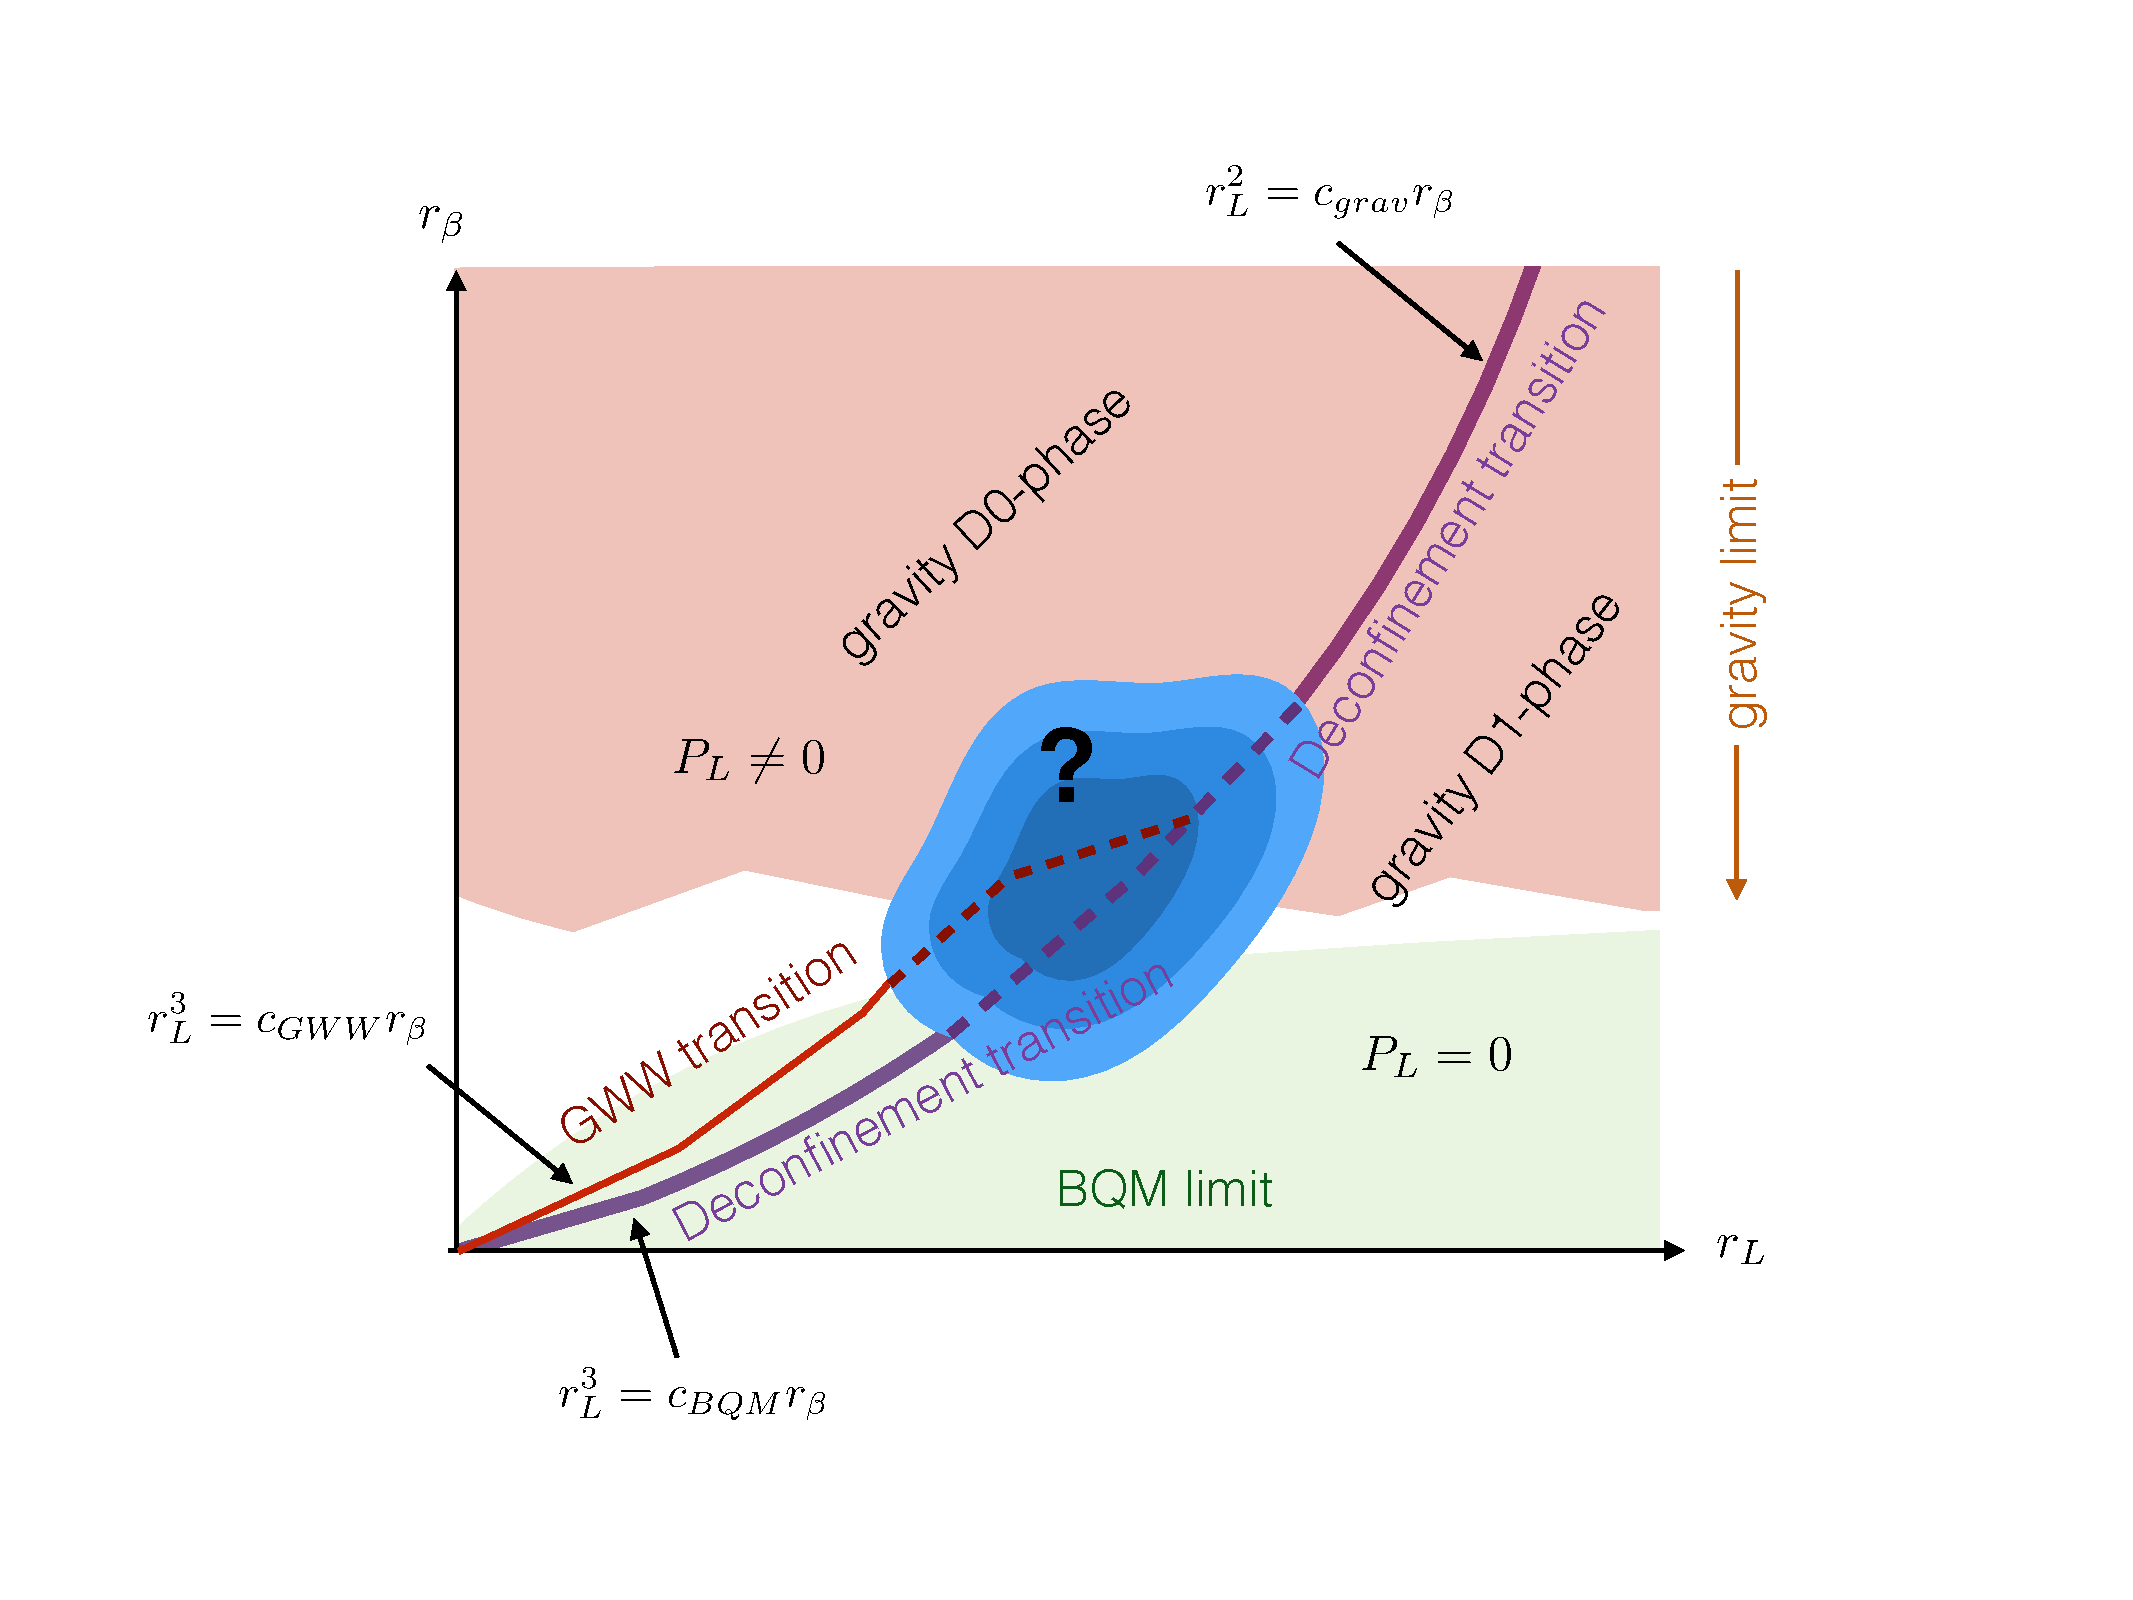
\includegraphics[width=\linewidth]{Figures/sum.pdf}
  \caption{\label{fig:summaryrect}Summary of the expected phase structure for the SYM theory on a rectangular 2-torus.}
\end{figure}

For large-$N$ two-dimensional SYM on a \emph{rectangular} Euclidean 2-torus we have two dimensionless parameters $r_{\beta}$ and $r_L$.
Assuming that $r_{\beta}, r_L \sim \cO(1)$ in the large-$N$ limit we have the following expectations:
\begin{itemize}
  \item The high-temperature, small-volume limit $r_{\beta}, r_L \ll 1$ is described by the dynamics of scalar and gauge zero modes.
        We expect $P_{\beta}, P_L \ne 0$ and $\vev{S_{\text{bos}}} \simeq -2N^2$.
  \item The high-temperature limit $r_{\beta}^3 \ll r_L$ reduces to BQM.
        Here we expect $P_{\beta} \ne 0$.
        For $r_L^3 < c_{\text{BQM}} r_{\beta}$ with $c_{\text{BQM}} \simeq 1.4$ we expect $P_L \ne 0$, with a deconfinement transition to $P_L = 0$ for $r_L^3 > c_{\text{BQM}} r_{\beta}$.
  \item The low-temperature limit, $r_{\beta} \gg 1$, admits a gravity-dual black hole description, so $P_{\beta} \ne 0$, with the free energy density depending on the ratio $r_L^2 / r_{\beta}$.
        For $r_L^2 = \cgrav r_{\beta}$, with $\cgrav = 2.45$ there is a first-order deconfinement phase transition with respect to $P_L$.
        The D1~phase, for $r_L^2 > \cgrav r_{\beta}$, has free energy density given by eq.~\eqref{eq:D1phase} and $P_L = 0$.
        The D0~phase, for $r_L^2 < \cgrav r_{\beta}$, has $P_L \ne 0$ with the free energy density well approximated by eq.~\eqref{eq:D0phase}.
\end{itemize}
This is illustrated in figure~\ref{fig:summaryrect}.

%------------------------
\section{\label{sec:skewed}Behaviour on a skewed torus}
We now discuss what happens to the Euclidean theory when it is placed on a skewed torus.
The motivation is twofold.
First, we emphasize that skewing the torus provides a new direction to deform the theory and hence a new independent test of holography, given again that gravity dual predictions exist.
Second, modern supersymmetric lattice constructions often naturally live on non-hypercubic lattices, which in turn are naturally adapted to giving a continuum Euclidean theory on a skewed torus.

We take the SYM to live on the flat 2-torus generated as a quotient of the two-dimensional plane.
Writing the metric as
\begin{equation}
  ds^2_{T^2} = d\tau^2 + dx^2,
\end{equation}
this is generated by the identifications
\begin{align}
  (\tau, x) & \sim (\tau, x) + \vec{\beta} & & \text{fermions anti-periodic} \\
  (\tau, x) & \sim (\tau, x) + \vec L & & \text{fermions periodic}
\end{align}
for vectors $\vec{\beta}$ ($\vec L$) about the thermal (spatial) circles with anti-periodic (periodic) fermion BCs.
These vectors defining the cycles have lengths and dot product
\begin{align}
  \beta & = |\vec{\beta}| &
  L & = |\vec L| &
  \ga & = \frac{\vec{\beta} \cdot \vec L}{\beta L}
\end{align}
with $|\ga| < 1$ to ensure a non-degenerate torus.
Thus the geometry is determined by three parameters---in addition to the $\beta$ and $L$ of the rectangular case there is the dimensionless skewing parameter $\ga$.
For any value of \ga (not just the rectangular case $\ga = 0$) we will be able to compare our numerical SYM results to gravity predictions, and hence test holography.

We have constructed the torus by a quotient of the plane by the vectors $\vec{L}$ and $\vec{\beta}$.
However, any SL$(2, \mathbb{Z})$ transformation of these vectors will define the \emph{same} geometric torus.
The anti-periodic BCs about the $\beta$ circle, and periodic ones about $L$, complicate this slightly.
Consider the transformation generated by the following subgroup of SL$(2, \mathbb{Z})$:
\begin{align}
  \label{eq:SLtransform}
  \left(\begin{array}{c}
    \vec{L}' \\
    \vec{\beta}'
  \end{array}\right) & = M \cdot \left(\begin{array}{c}
    \vec{L} \\
    \vec{\beta}
  \end{array}\right) &
  M & = \left(\begin{array}{cc}
    a & 2n \\
    c & 2m - 1
  \end{array}\right) \in \text{SL}(2, \mathbb{Z}), &
  n, m, c & \in \mathbb{Z},
\end{align}
where we note that then $a \in 2\mathbb{Z} - 1$.
Then the 2-torus defined by $\vec{\beta}'$ (anti-periodic fermions) and $\vec{L}'$ (periodic fermions) is the \emph{same} as that defined by $\vec{\beta}$ and $\vec{L}$.
The fermion BCs restrict us to a subgroup of the full SL action, so that the new $\vec{\beta}'$ has an odd coefficient multiplying $\vec{\beta}$ to maintain anti-periodicity, and likewise $\vec{L}'$ has an even coefficient multiplying $\vec{\beta}$.

In the rectangular case, we have a Lorentzian thermal interpretation of the physics, where we identify $\beta$ as inverse temperature in a canonical ensemble.
In the skewed case, this is no longer true.
Nonetheless, we may regard this case as a generalized thermal ensemble, with $1 / \beta$ playing the role of generalized temperature.
As for a rectangular torus, we again work with dimensionless
\begin{align}
  r_{\beta} & = \beta \sqrt{\lam} &
  r_L & = L \sqrt{\lam},
\end{align}
now supplemented by the dimensionless parameter $\ga$.
We denote $t = 1 / r_{\beta}$ the generalized dimensionless temperature, and also define the aspect ratio
\begin{equation}
  \al = \frac{L}{\beta} = \frac{r_L}{r_{\beta}}.
\end{equation}
The 2-volume is then given as $\text{Vol}_{T^2} = \beta^2 \al \sqrt{1 - \ga^2}$.
In practice on the lattice, it will be convenient to scan the parameter space by fixing the `shape' of the torus set by $(\al, \ga)$ and varying the dimensionless temperature $t$ that controls the size of the torus in units of the SYM coupling $\lam$.

The redundancy in our description of the torus using $\vec{\beta}$ and $\vec{L}$ given in~\eqref{eq:SLtransform} translates into an invariance in this parameterization: a set $\al, \ga, t$ defined from $\vec{\beta}$ and $\vec{L}$ is equivalent to other parameters $\al', \ga', t'$ similarly defined from $\vec{\beta}'$ and $\vec{L}'$.
In the usual manner we may describe this using the complex `modular parameter' $\uptau$, given by\footnote{Since `tau' is conventionally used for both the torus modular parameter and Euclidean time, we attempt to avoid potential confusion by using the symbols $\uptau$ for the modular parameter and $\tau$ for Euclidean time.}
\begin{equation}
  \uptau = \frac{L_{\tau} + iL_x}{\beta_{\tau} + i\beta_x} = \al \left(\ga + i\sqrt{1 - \ga^2}\right),
\end{equation}
which encodes the (dimensionless) shape parameters $\al, \ga$, and is independent of the torus scale.
The parameter transforms under the action~\eqref{eq:SLtransform} as
\begin{equation}
  \uptau' = \frac{a \uptau + 2n}{c \uptau + 2m - 1},
\end{equation}
so that $m, n, c \in \mathbb{Z}$ and $a(2m - 1) - 2nc = 1$.
We term this a \emph{restricted} modular transformation---it is a usual modular transformation, but restricted to preserve our fermion BCs (anti-periodic on the $\vec{\beta}$ cycle and periodic on the $\vec{L}$ cycle).
As for the usual modular invariance of the torus, we may define a fundamental domain for this $\uptau$ parameter under the action of this restricted transform~\eqref{eq:SLtransform}, which gives the set of inequivalent tori (taking into account fermion BCs).
A modular parameter outside this domain can then be mapped back into it using the appropriate~\eqref{eq:SLtransform}.
The usual modular transformations are generated by $\uptau \to \uptau + 1$ and $\uptau \to -1 / \uptau$, or equivalently $\uptau \to \uptau + 1$ and $\uptau \to \frac{\uptau}{\uptau + 1}$.
We provide some review of this in appendix~\ref{app:modular}.
However for our restricted transform instead we may use the generators $\uptau \to \uptau + 2$ and $\uptau \to \frac{\uptau}{\uptau + 1}$.
The fundamental domain $D$ may then be taken to be
\begin{equation}
  D = \left\{\uptau\big|1 \le |\uptau \pm 1|, \; |\mathrm{Re}(\uptau)| \le 1\right\}.
\end{equation}
These assertions are proved in appendix~\ref{app:modular}.
The lattice construction we use later will give torus geometries with a particular \ga (which we will see is $\ga = -1 / 2$), and we will vary the shape parameter \al of the torus and its size $t$.
Some of the torus shapes we study will correspond to $\uptau$ within the fundamental domain, and others will not.
We will generally present results in terms of \al and $t$ for this common value of $\ga$, but as we discuss later, for the shapes that fall outside the fundamental domain there is an alternate description with new $\al', \ga', t'$.\footnote{It is worth emphasizing that the way the modular parameter $\uptau$ arises is a little different to that in the familiar two-dimensional CFT setting.  In the context of Euclidean two-dimensional CFT \emph{any} 2-torus is Weyl equivalent to a flat torus with modular parameter $\uptau$ (i.e., one constructed as a quotient of the two-dimensional plane) and unit volume.  Hence for \emph{any} 2-torus the CFT partition function \emph{only} depends on the geometry through $\uptau$.  However in our case, the SYM is not a CFT---in particular, our theory explicitly depends on the size of the torus, and will also depend on the details of its real geometry.  We restrict ourselves to only consider 2-tori constructed as quotients of the plane, which are flat but with a skewing parameterized by $\uptau$.  Hence our SYM depends on $\uptau$ and the scale (through, say, $\beta$) because we have restricted to flat tori.  If we also added scalar curvature the situation would be more complicated (unlike for a CFT).  However in either case (CFT or our SYM), the dependence is on $\uptau$ up to modular invariance, so we may always choose $\uptau$ to be in the fundamental domain.  This is simply because the description of the torus has this invariance, and it is \emph{not} due to any symmetry properties of the field theory.}

An important aim of our lattice calculations is to see the detailed generalized thermodynamic behavior predicted by the dual black holes.
However, in a skewed setting we are no longer in a strict thermal context and so potentials such as free energy are not strictly meaningful.
Instead, the relevant quantity is the (logarithm of the) partition function
\begin{equation}
  \label{eq:partfunc}
  Z[t, \al, \ga] = \int D(\text{fields}) \, e^{-S}
\end{equation}
for the Euclidean action given by eq.~\eqref{eq:SYMaction}, but now on the skewed 2-torus.
In a lattice calculation it is hard to determine the value of this integral directly, so instead, we focus on expectation values, which are much more convenient to compute.
A natural observable is the expectation value of the Euclidean action $S$.
Since the fermionic part of the action is Gaussian, its value is simply a constant.
Therefore we will focus on measuring the expectation value of the bosonic part of the action, $S_{\text{Bos}}$, given in eq.~\eqref{eq:SYMaction}.
We will find it convenient to work with the average bosonic action \emph{density}, defined from the (renormalized) vev of $S_{\text{Bos}}$ in an obvious way,
\begin{equation}
  \vev{s_{\text{Bos}}} = \frac{1}{\text{Vol}_{T^2}} \vev{S_{\text{Bos}}}.
\end{equation}
We now show that $s_{\text{Bos}}$ is related to a derivative of the partition function $\ln Z$.
After scaling the bosonic fields and coordinates as
\begin{align}
  \tau' & = \frac{1}{\beta} \tau &
  x' & = \frac{1}{\beta} x &
  A_{\mu}' & = \beta A_{\mu} &
  X_i' & = \beta X_i,
\end{align}
the Euclidean action becomes
\begin{align}
  S_{\text{Bos}} & = \frac{N}{\beta^2 \lam} I[\al, \ga] \cr
  I[\al, \ga] & = \int_{T'^2} d\tau' \, dx' \, \Tr{\frac{1}{4} F_{\mu\nu}' F'^{\mu\nu} + \frac{1}{2} (D_{\mu}' X_i')^2 - \frac{1}{4} [X_i', X_j']^2}.
\end{align}
The 2-torus $T'^2$ is generated by the identifications
\begin{align}
  (\tau', x) & \sim (\tau' + 1, x) &
  (\tau', x) & \sim (\tau' + \ga \al, x + \al\sqrt{1 - \ga^2}),
\end{align}
the former anti-periodic and the latter periodic for the fermions.
Thus we have scaled out $\beta$.
The only explicit $\beta$ dependence is in the overall coupling, and the integral $I[\al, \ga]$ depends only on the dimensionless shape parameters \al and \ga (through the identifications above).
By suitably scaling the fermion fields the fermionic action can be chosen to have no $\beta$ dependence.
Then differentiating the partition function with respect to $\beta$, keeping \al and \ga fixed, we obtain
\begin{align}
  \left. \beta \pderiv{}{\beta} \ln Z \right|_{\al, \ga} & = \frac{1}{Z} \int D(\text{fields}) \left(\left. \beta \pderiv{}{\beta} \left(-\frac{N}{\beta^2 \lam} I[\al, \ga]\right) \right|_{\al, \ga}\right) e^{-S} = 2\vev{S_{\text{Bos}}} \\
  \vev{s_{\text{Bos}}} & = \frac{1}{2 \text{Vol}_{T^2}} \left. \beta \pderiv{}{\beta} \ln Z \right|_{\al, \ga}.                                                                                                             \label{bosonicaction}
\end{align}
Thus computing $s_{\text{Bos}}$ as a function of $t$, \al and $\ga$, which may be conveniently done on the lattice, gives the same information as that contained in the partition function.

As in the rectangular case, we will be interested in the Wilson loops about the torus temporal and spatial cycles and their magnitudes $P_{\beta}$ and $P_L$, respectively.
Since there are equivalent presentations of the same torus, one can equally consider the loops $P_{\beta}'$ and $P_L'$, which correspond to cycles in the original representation that wrap multiples of the cycles generated by $\vec{\beta}$ and $\vec{L}$.

We now proceed to discuss the same limits as in the rectangular case in this skewed geometry.
We will find that analogous small circle reductions occur, and that generalized black holes still give gravity predictions for small generalized temperature $1 \ll r_{\beta}$.
We first discuss the dimensional reduction of the theory on a skewed torus, and then turn to a discussion of the gravity dual, giving predictions for the observable $s_{\text{Bos}}$.

%------------------------
\subsection{\label{sec:smallcircle}High-temperature limit}
We now take the skewing parameter \ga to be fixed and consider the high-temperature limit, finding qualitatively similar behavior to the rectangular torus case we previously discussed.
In the small-volume, high-temperature limit $r_{\beta}, r_L \ll 1$ precisely the same reduction to the matrix integral occurs.
Thus we again expect $P_{\beta} \simeq P_L \ne 0$, with the bosonic action behaving as $\vev{S_{\text{Bos}}} / N^2 \simeq -2$ at large $N$.
Translating to the bosonic action density we then obtain
\begin{equation}
  \label{eq:HT}
  \frac{\vev{s_{\text{Bos}}}}{N^2 \lam} = -\frac{2}{\al \sqrt{1 - \ga^2}} t^2.
\end{equation}

At finite volume, we may again reduce to an effective one-dimensional theory at high temperature.
The easiest way to understand this dimensional reduction is to note that skewed tori in the fixed-$\ga$, high-temperature limit become equivalent to nearly rectangular tori (again with small thermal circles) under a suitable transformation~\eqref{eq:SLtransform}.
Then we may simply dimensionally reduce this equivalent rectangular torus, and pull the result back to the original skewed torus parameterization given by $\ga$.

Thus we consider the high-temperature limit where we fix \ga and $r_L$, taking $r_{\beta} \to 0$ so that $\al \to \infty$.
We use the transform~\eqref{eq:SLtransform} with $c = 0$, $m = 0$ and $a = 1$, leaving $n \in \mathbb{Z}$, to find an equivalent torus that will be approximately rectangular.
This maps $\vec{\beta}$, $\vec{L}$ to
\begin{align}
  \vec{\beta}' & = \vec{\beta} &
  \vec{L}' & = \vec{L} + 2n \vec{\beta}.
\end{align}
This leaves the temperature unchanged, $t' = t$, and relates the shape parameters as
\begin{align}
  \al' \ga' & = \al \ga + 2n &
  \al' \sqrt{1 - \ga'^2} & = \al \sqrt{1 - \ga^2}.
\end{align}
In the $\al \to \infty$ limit we may choose $n$ appropriately (i.e., taking $-\al \ga / 2 \simeq n \in \mathbb{Z}$) to obtain an equivalent torus with $\ga' \simeq 0$ and $\al' \simeq \al \sqrt{1 - \ga^2} \to \infty$.
This equivalent torus is approximately rectangular and in the high-temperature limit, so from our previous discussion in section~\ref{sec:rectHighTemp} we may reduce the thermal circle when
\begin{equation}
  \label{eq:reductime}
  \left(r_{\beta}' \right)^3 \ll r_L' \quad \implies \quad r_{\beta}^3 \ll r_L \sqrt{1 - \ga^2}.
\end{equation}
We obtain a bosonic quantum mechanics (BQM) on a circle size $L_{\text{BQM}} = L'$ with coupling $\lam_{\text{BQM}} = \lam / \beta'$, so that
\begin{align}
  \lam_{\text{BQM}} & = \frac{\lam}{\beta} &
  L_{\text{BQM}} & = L \sqrt{1 - \ga^2}.
\end{align}
Thus we have the same relation of the lower- and higher-dimensional coupling as in the rectangular case, but the circle size is related via a skewing-dependent factor.

Reducing on the thermal cycle $\vec{\beta}'$ implies that the Polyakov loop is $P_{\beta}' \sim 1$.
Given that $P_{\beta}' = P_{\beta}$, and this Polyakov loop is trivial, we expect thermal deconfinement, $P_{\beta} \ne 0$.
Then $P_L \simeq P_L' = P_{\text{BQM}}$, so our previous discussion of BQM implies the deconfinement transition in the limit of eq.~\eqref{eq:reductime} is located at
\begin{equation}
  \label{eq:skewBQM}
  r_L^3 \simeq \frac{1.4}{\left(1 - \ga^2\right)^{\frac{3}{2}}} r_{\beta}.
\end{equation}
This is associated with a transition from a spatially confined phase with $P_L = 0$ to a deconfined one with $P_L \ne 0$ as $r_L^3 / r_{\beta}$ is reduced.

%------------------------
\subsection{The low-temperature dual gravity limit - D1 phase}
Considering the dual IIB gravity we find the same homogeneous D1-charged black hole solution as in eq.~\eqref{eq:IIBmetric}, but now we take the two-dimensional torus in the field theory directions to be generated by the identifications
\begin{align}
  \label{eq:IIBident}
  (\tau, x) & \sim (\tau + \beta, x)                     & & \text{anti-periodic fermions} \cr
  (\tau, x) & \sim (\tau + \ga L, x + L\sqrt{1 - \ga^2}) & & \text{periodic fermions.}
\end{align}
Then asymptotically, when $U_0 \gg U$, the torus spanned by $\tau$ and $x$ has our required skewed geometry.
We also see that the relation between $U_0$ and $\beta$ is exactly the same as for eq.~\eqref{eq:IIBmetric}, since the metric is locally the same as in the rectangular case, and the $\tau$ circle has the same period $\beta$.

We will regard this as a `generalized black hole' in the sense that for real $\beta$ and $\ga \ne 0$ its properties are not related directly to a physical Lorentzian black hole.
Nonetheless, the Euclidean IIB solution exists.
The geometry of this solution differs only globally in the $x$ direction from the rectangular case and is homogeneous in $x$.
The solution should be a good description of the IIB string theory again for large $N$ and $1 \ll r_{\beta}$.
We expect it to become unstable to a winding mode instability for $r_L^2 \sim r_{\beta}$.

Consider the expectation value of the SYM Euclidean Lagrangian density $\vev{L_E}$ predicted by this solution, which will be homogeneous in both $\tau$ and $x$.
Then $-\ln Z = \vev{S} = \text{Vol}_{T^2} \vev{L_E}$ when this black hole is the dominant saddle point of the path integral.
Due to the homogeneity in $x$ this Lagrangian density is only a function of $\beta$, and has no dependence on the other parameters \al and \ga determining the shape of the torus.
In the rectangular case it simply equals the free energy density of the solution, and thus generally is given by eq.~\eqref{eq:D1phase}, so $\vev{L_E} = -N^2 \lam \cdot 2^4 \pi^{\frac{5}{2}} t^3 / 3^4$.
As before we refer to this homogeneous black string phase as the \emph{D1~phase}.
Hence if this gravitational solution dominates the partition function the theory is in the D1~phase and the bosonic action density is
\begin{equation}
  \label{eq:skewD1phase}
  \text{D1~phase:} \quad \frac{s_{\text{Bos, D1}}}{N^2 \lam} = -\frac{1}{2 \text{Vol}_{T^2}} \left. \beta \pderiv{}{\beta} \left(\text{Vol}_{T^2} \vev{L_E}\right) \right|_{\al, \ga} = -\frac{2^3 \pi^{\frac{5}{2}}}{3^4} t^3 \simeq -1.728t^3.
\end{equation}
We see explicitly that our observable doesn't depend on the skewing of the torus.
As in the rectangular case, $\partial / \partial \tau$ generates a contractible cycle due to the horizon.
Now the Euclidean time cycle of the torus is simply generated by $\partial / \partial \tau$.
The spatial cycle of the torus is now generated by $\sqrt{1 - \ga^2} \partial / \partial x + \ga \partial / \partial \tau$, and since $\partial / \partial x$ is not contractible, neither is this spatial torus cycle.
Thus when eq.~\eqref{eq:IIBmetric} is the dominant bulk solution, this implies that the Polyakov loop $P_{\beta} \ne 0$, whereas $P_L = 0$.
Hence the dual SYM is thermally deconfined but in a spatially confined phase.

There is an important subtlety in the above discussion: one must be careful whether the solution above~\eqref{eq:IIBmetric} does dominate, due to there being other related gravitational dual black holes~\cite{Aharony:2005ew}.
In eq.~\eqref{eq:IIBident} we have identified with $\vec{\beta}$ and $\vec{L}$ to generate the 2-torus, but as discussed in ref.~\cite{Aharony:2005ew} we may equally well use any equivalent pair under the transformation~\eqref{eq:SLtransform}, since they will give the same flat 2-torus asymptotically.
This will yield another inequivalent gravitational dual solution.
However, it is the pair of vectors whose corresponding modular parameter $\uptau$ lies in the fundamental domain that gives the dominant gravitational dual solution.
This is understood as follows.
Take a $\uptau$ in the fundamental domain, $D$, and a temperature $t$.
Then the Euclidean action density is as in eq.~\eqref{eq:skewD1phase}.
Now transforming this to an equivalent $\uptau'$ outside the fundamental domain results in a new dimensionless temperature $t'$ given in terms of $t$, $\uptau$ and the transformation.
This $t'$ is lower than the fundamental-domain temperature $t$ since\footnote{Eq.~\eqref{eq:treln} may be derived neatly by noting the 2-torus volume $\beta^2 \mathrm{Im}(\uptau)$ is invariant under modular transformations.}
\begin{equation}
  \label{eq:treln}
  \left(\frac{t'}{t}\right)^2 = \frac{\mathrm{Im}(\uptau')}{\mathrm{Im}(\uptau)},
\end{equation}
and from the corollary in appendix~\ref{app:modular} we have $\mathrm{Im}(\uptau') / \mathrm{Im}(\uptau) \le 1$ for $\uptau \in D$.
Thus we see $t' \le t$.
Hence the action density of these other gravitational saddle points, which is given by~\eqref{eq:skewD1phase} with $t \to t'$, is more positive.
Since the volume of the torus is preserved under the modular transformation~\eqref{eq:SLtransform}, then the Euclidean action is also more positive.
Thus these other dual solutions outside the fundamental domain are not the relevant saddle points to determine the partition function behavior.

Hence the subtlety is that the D1-phase prediction is given by eq.~\eqref{eq:skewD1phase} for $\al, \ga, t$ corresponding to a $\uptau$ in the fundamental domain.
If one has a set of parameters outside the fundamental domain, one must first map them to new parameters $\al', \ga', t'$ in the fundamental domain, and then apply the formula~\eqref{eq:skewD1phase} with $t \to t'$.\footnote{The expression \eqref{eq:skewD1phase} could not hold for general $\al, \ga, t$ as it would not respect the modular invariance that the SYM on this flat torus must enjoy.  It is also worth emphasizing that one cannot naively compare eqs.~\eqref{eq:skewD1phase} and \eqref{eq:skewD0phase} to deduce a critical temperature, since $\uptau \not\in D$ when the latter is valid.}
In this canonical representation (i.e., $\uptau' \in D$) we will have the prediction $P_{\beta}' \ne 0$ and $P_L' = 0$ for the Wilson loops.
A spatial cycle of the torus is always non-contractible, so we should have $P_L = 0$ in any equivalent representation.
However, while $P_{\beta}' \ne 0$ for the thermal cycle in the fundamental domain representation, if in the equivalent representation $\vec{\beta}$ is a linear combination of both $\vec{\beta}'$ and $\vec{L}'$ it may correspond to a non-contractible cycle in the gravity dual, so that also $P_{\beta} = 0$.
We emphasize that this does \emph{not} imply temporal confinement, since there is \emph{some} temporal loop (associated to the cycle $\vec{\beta}'$) where $P_{\beta}' \ne 0$.

%------------------------
\subsection{The low-temperature dual gravity limit - D0 phase}
Considering the D1~phase with $r_{\beta} \gg 1$ where the gravity is a valid description, fixing \ga and reducing the circle size to $r_L^2 \sim r_{\beta}$ we again expect winding modes on the spatial circle to become important near the horizon, as in section~\ref{sec:dualGrav}.
This limit, however, is straightforward to understand, as it implies $r_L \ll r_{\beta}$ and thus we may play a similar trick as for the small-thermal-circle dimensional reduction in section~\ref{sec:smallcircle}, again mapping to an equivalent almost-rectangular representation.
We set $a = 1$, $n = 0$ and $m = 0$ in the transform~\eqref{eq:SLtransform}, leaving $c \in \mathbb{Z}$.
Then
\begin{align}
  \vec{\beta}' & = \vec{\beta} + c \vec{L} &
  \vec{L}' & = \vec{L},
\end{align}
so $L' = L$ and the equivalence relates the shape parameters as
\begin{align}
  \label{eq:circred}
  \frac{1}{\al'} \ga' & = \frac{1}{\al} \ga + c &
  \frac{1}{\al'} \sqrt{1 - \ga'^2} & = \frac{1}{\al} \sqrt{1 - \ga^2}.
\end{align}
Then by choosing $c$ appropriately (i.e., taking $-\ga / \al \simeq c \in \mathbb{Z}$) in the $\al \to 0$ limit we obtain an equivalent torus with $\ga' \simeq 0$ and $\al' = \al / \sqrt{1 - \ga^2} \to 0$.

Thus for fixed non-zero \ga and $r_L \ll r_{\beta}$, so that the modular parameter $\uptau$ is far outside the fundamental domain, the above transform maps to an approximately rectangular torus with $r_L' = r_L$ and $r_{\beta}' = r_{\beta} \sqrt{1 - \ga^2}$.
For the rectangular torus we know that the phase transition from the D0~phase to the D1~phase occurs for $r_L'^2 = \cgrav r_{\beta}'$ with $\cgrav = 2.45$.
Mapping this back to our non-rectangular parameterization, we expect a transition at
\begin{equation}
  \label{eq:skewtransition}
  r_L^2 = \cgrav \sqrt{1 - \ga^2} r_{\beta}.
\end{equation}
Then for this rectangular torus we may use the approximation~\eqref{eq:D0phase} for the thermal behavior, replacing $t \to t'$.
From this we may compute $\ln Z$.
Translating back to our original temperature $t$ we may compute the bosonic action density using eq.~\eqref{bosonicaction} to obtain, in our original non-rectangular parameterization,
\begin{align}
  \label{eq:skewD0phase}
  \frac{s_{\text{Bos}}}{N^2 \lam} = -\left(\frac{2^{21} \cdot 3^7 \cdot 5^2 \pi^{14}}{7^{19}}\right)^{\frac{1}{5}} \frac{t^{\frac{16}{5}}}{\al^{\frac{2}{5}} \left(1 - \ga^2\right)^{\frac{7}{5}}} \Bigg[1 - & \left(\frac{2^{11} \cdot 3^2 \cdot 5^2}{7^{14} \pi^{21} \left(1 - \ga^2\right)^7}\right)^{\frac{1}{5}} \zeta(7) \left(\frac{\al^2}{t}\right)^{\frac{14}{5}} \cr
  + & \cO\left(\left(\frac{\al^2}{t}\right)^{\frac{28}{5}}\right)\Bigg].
\end{align}
In the rectangular representation when this D0~phase dominates we expect to have $P_{\beta}', P_L' \ne 0$, so this phase is both spatially and thermally deconfined.
Furthermore, since $\vec{L}' = \vec{L}$ we also have $P_L \ne 0$.
Thus $P_L$ remains an order parameter for the transition between the gravity D1 and D0~phases.

%------------------------
\subsection{\label{sec:summaryskew}Summary for SYM on a skewed torus}
For large-$N$ SYM on a skewed torus with fixed $\ga$, upon varying $r_L$ and $r_{\beta}$ our expectation is a phase diagram similar to figure~\ref{fig:summaryrect} for the rectangular case.
We expect a spatial deconfinement transition line with order parameter $P_L$.
\begin{itemize}
  \item In the high-temperature, small-volume limit $r_{\beta}, r_L \ll 1$ we expect $P_L \ne 0$ and thermal behavior as in eq.~\eqref{eq:HT}.
  \item For high temperatures $r_{\beta}^3 \ll r_L$ the SYM may be dimensionally reduced to the BQM theory, leading us to expect the phase transitions described in eq.~\eqref{eq:skewBQM}.
        We will have $P_L \ne 0$ for $r_L^3 \lesssim 1.4 r_{\beta} / (1 - \ga^2)^{3 / 2}$, and $P_L = 0$ otherwise.
  \item For low temperatures $t \ll 1$ we expect a IIA or IIB gravity black hole description.
        The D0~phase, with approximate behavior~\eqref{eq:skewD0phase} and $P_L \ne 0$, dominates for $r_L^2 < \cgrav \sqrt{1 - \ga^2} r_{\beta}$.
        For $r_L^2 > \cgrav \sqrt{1 - \ga^2} r_{\beta}$ we expect the D1~phase with $P_L = 0$ to dominate with behavior~\eqref{eq:skewD1phase}, where this formula assumes $r_L$, $r_{\beta}$ and \ga are in the fundamental domain.
\end{itemize}
We expect all these phases to be thermally deconfined, so we may find a temporal cycle $\vec{\beta}'$ for which $P_{\beta}' \ne 0$.
For most phases this will be simply the $\vec{\beta}$ cycle, so $P_{\beta} \ne 0$.
However, as discussed above, for the D1~phase it is possible in the skewed case that $P_{\beta}$ may vanish.

\begin{figure}[tbp]
  \centering
  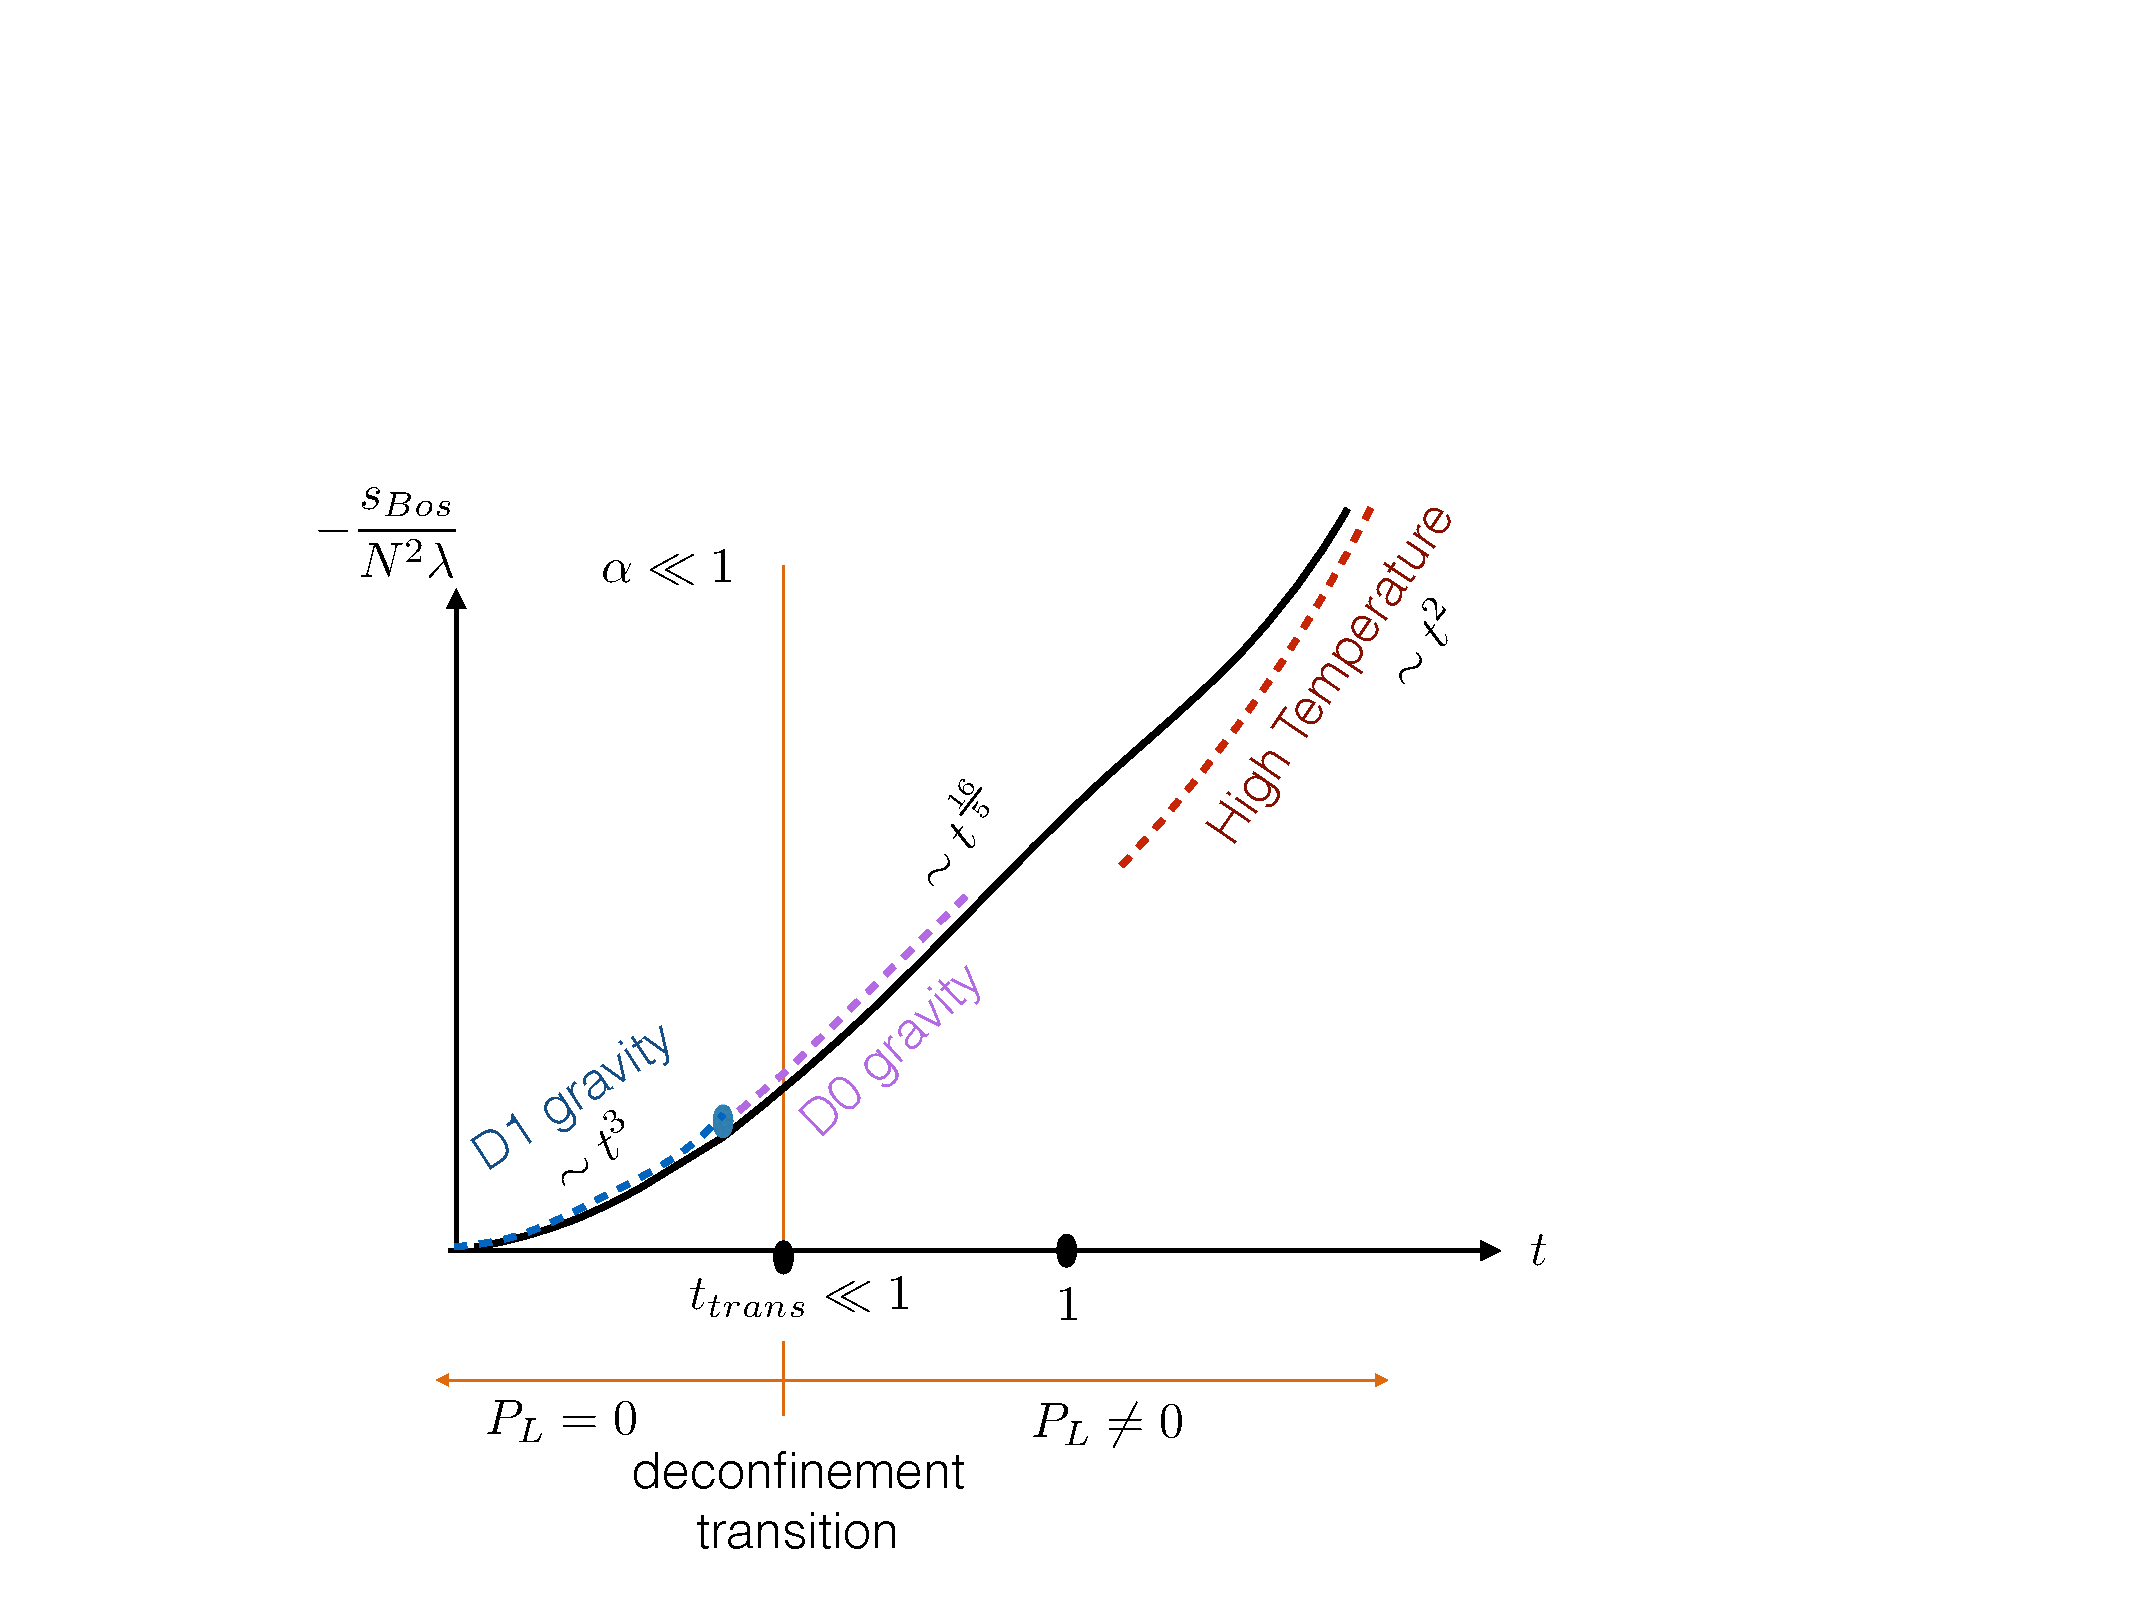
\includegraphics[height=6cm]{Figures/FigSummary2.pdf}\hfill 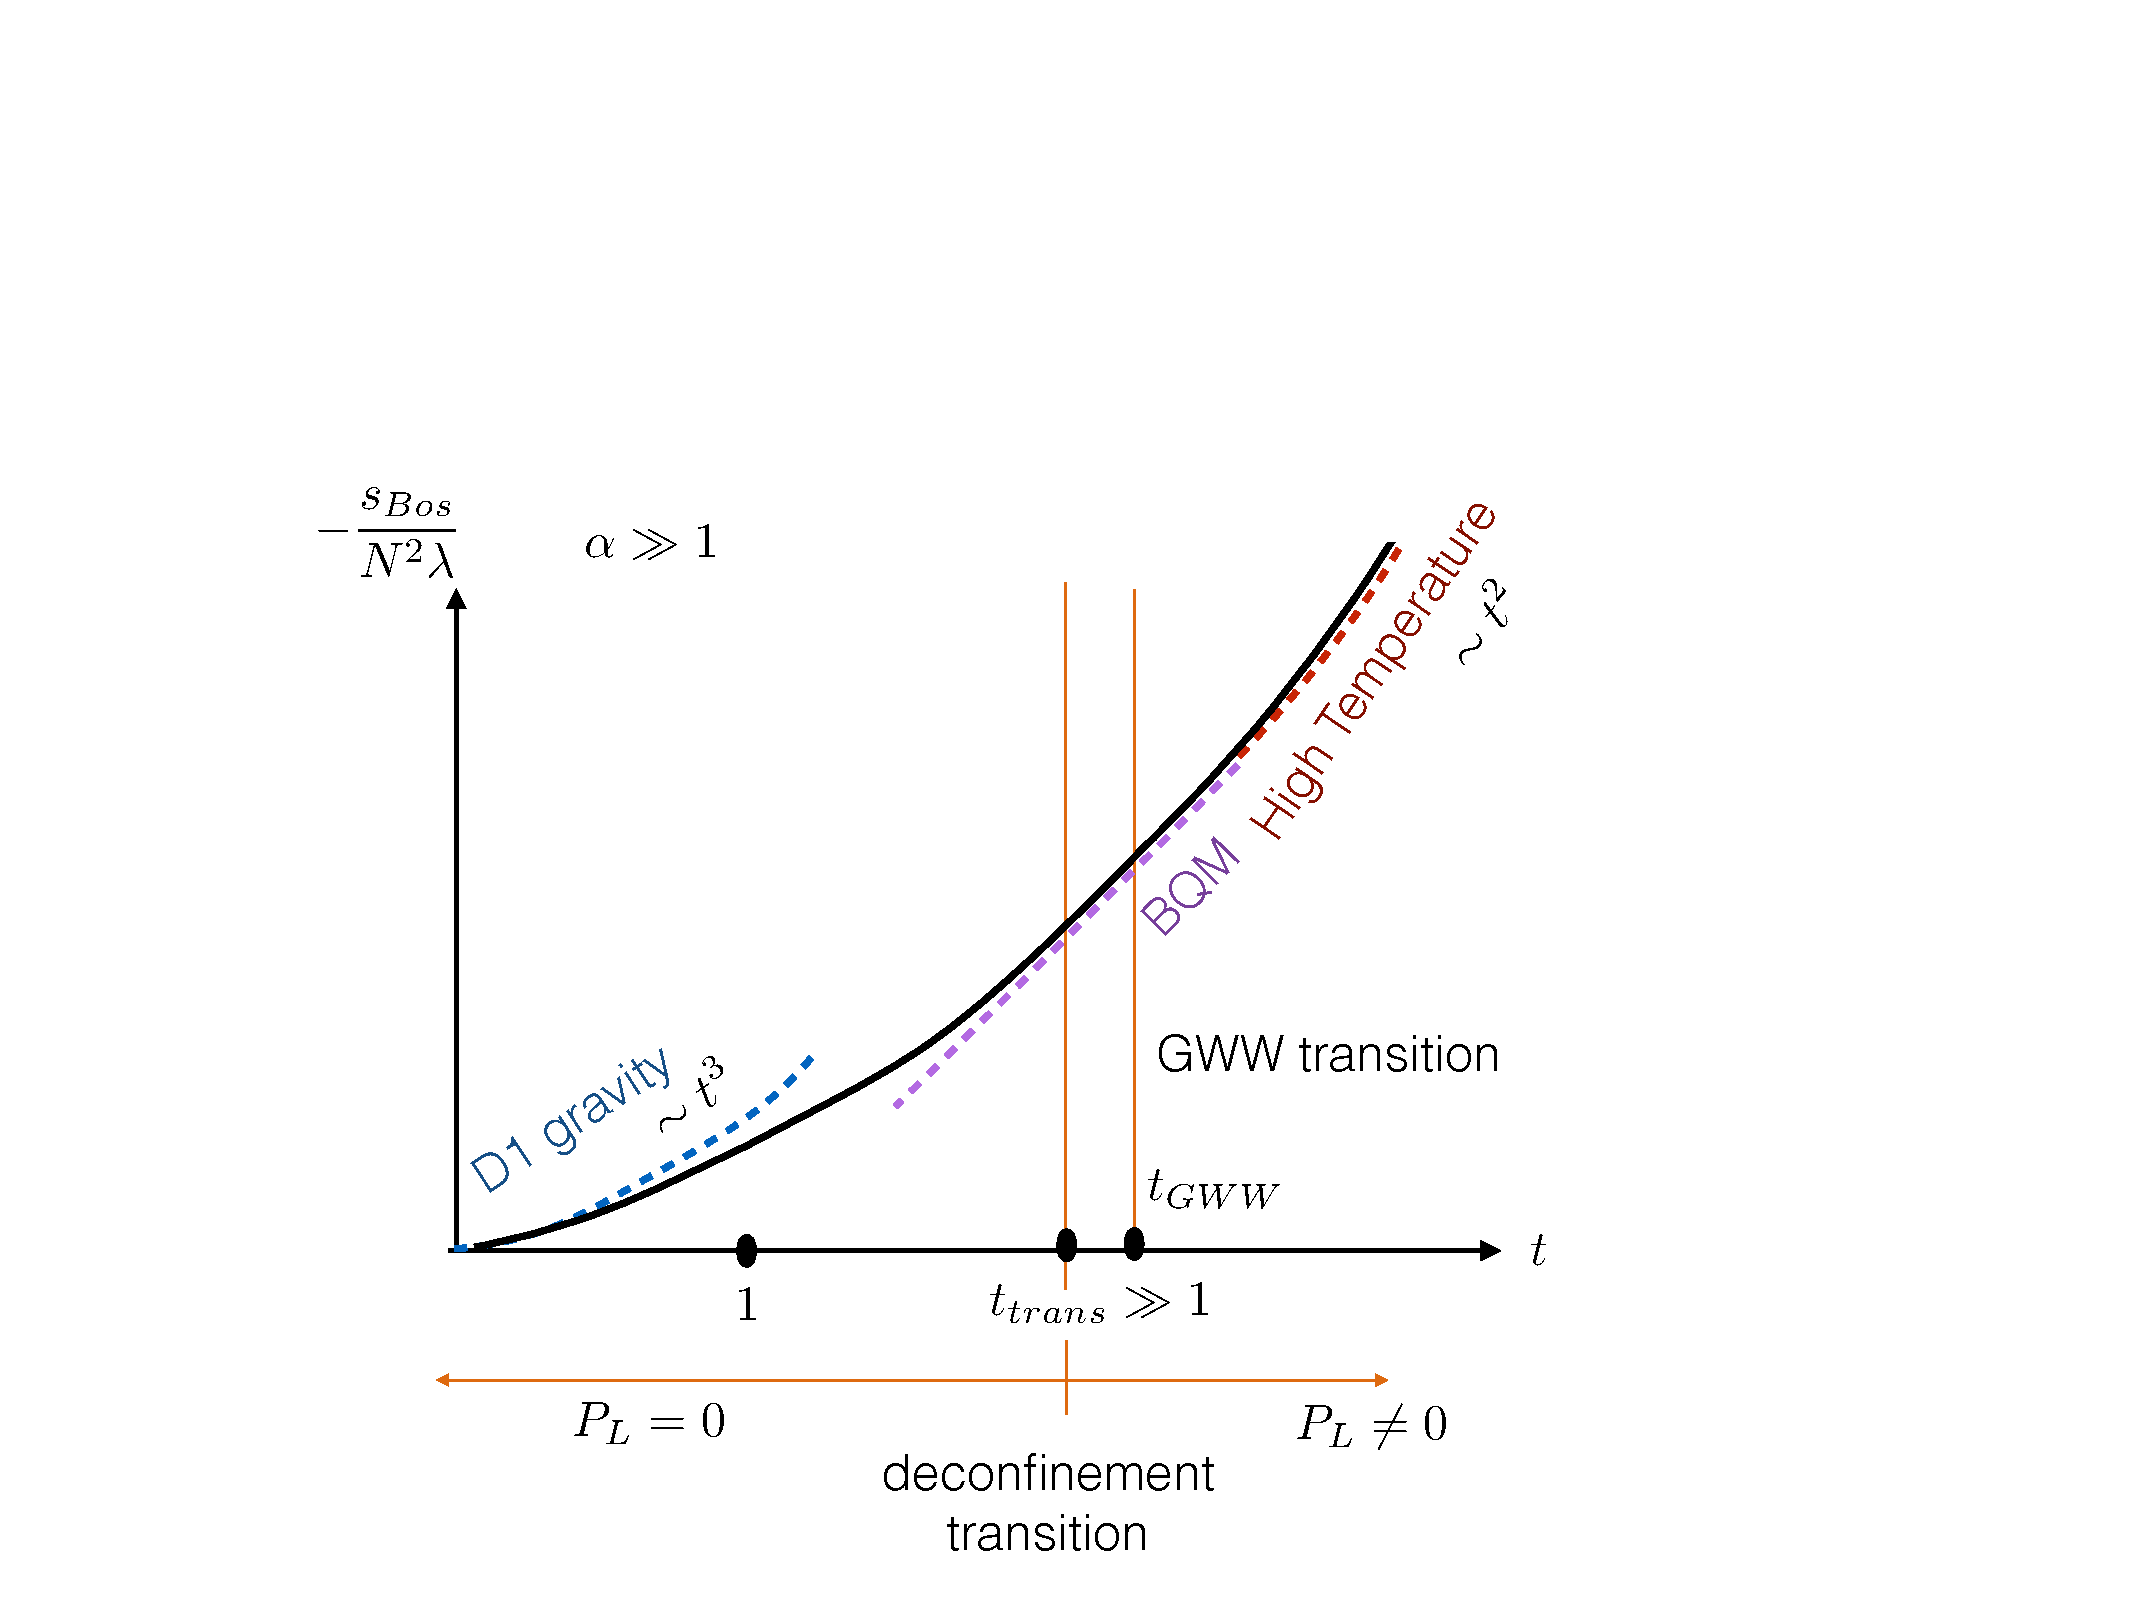
\includegraphics[height=6cm]{Figures/FigSummary3.pdf} \\[6 pt]
  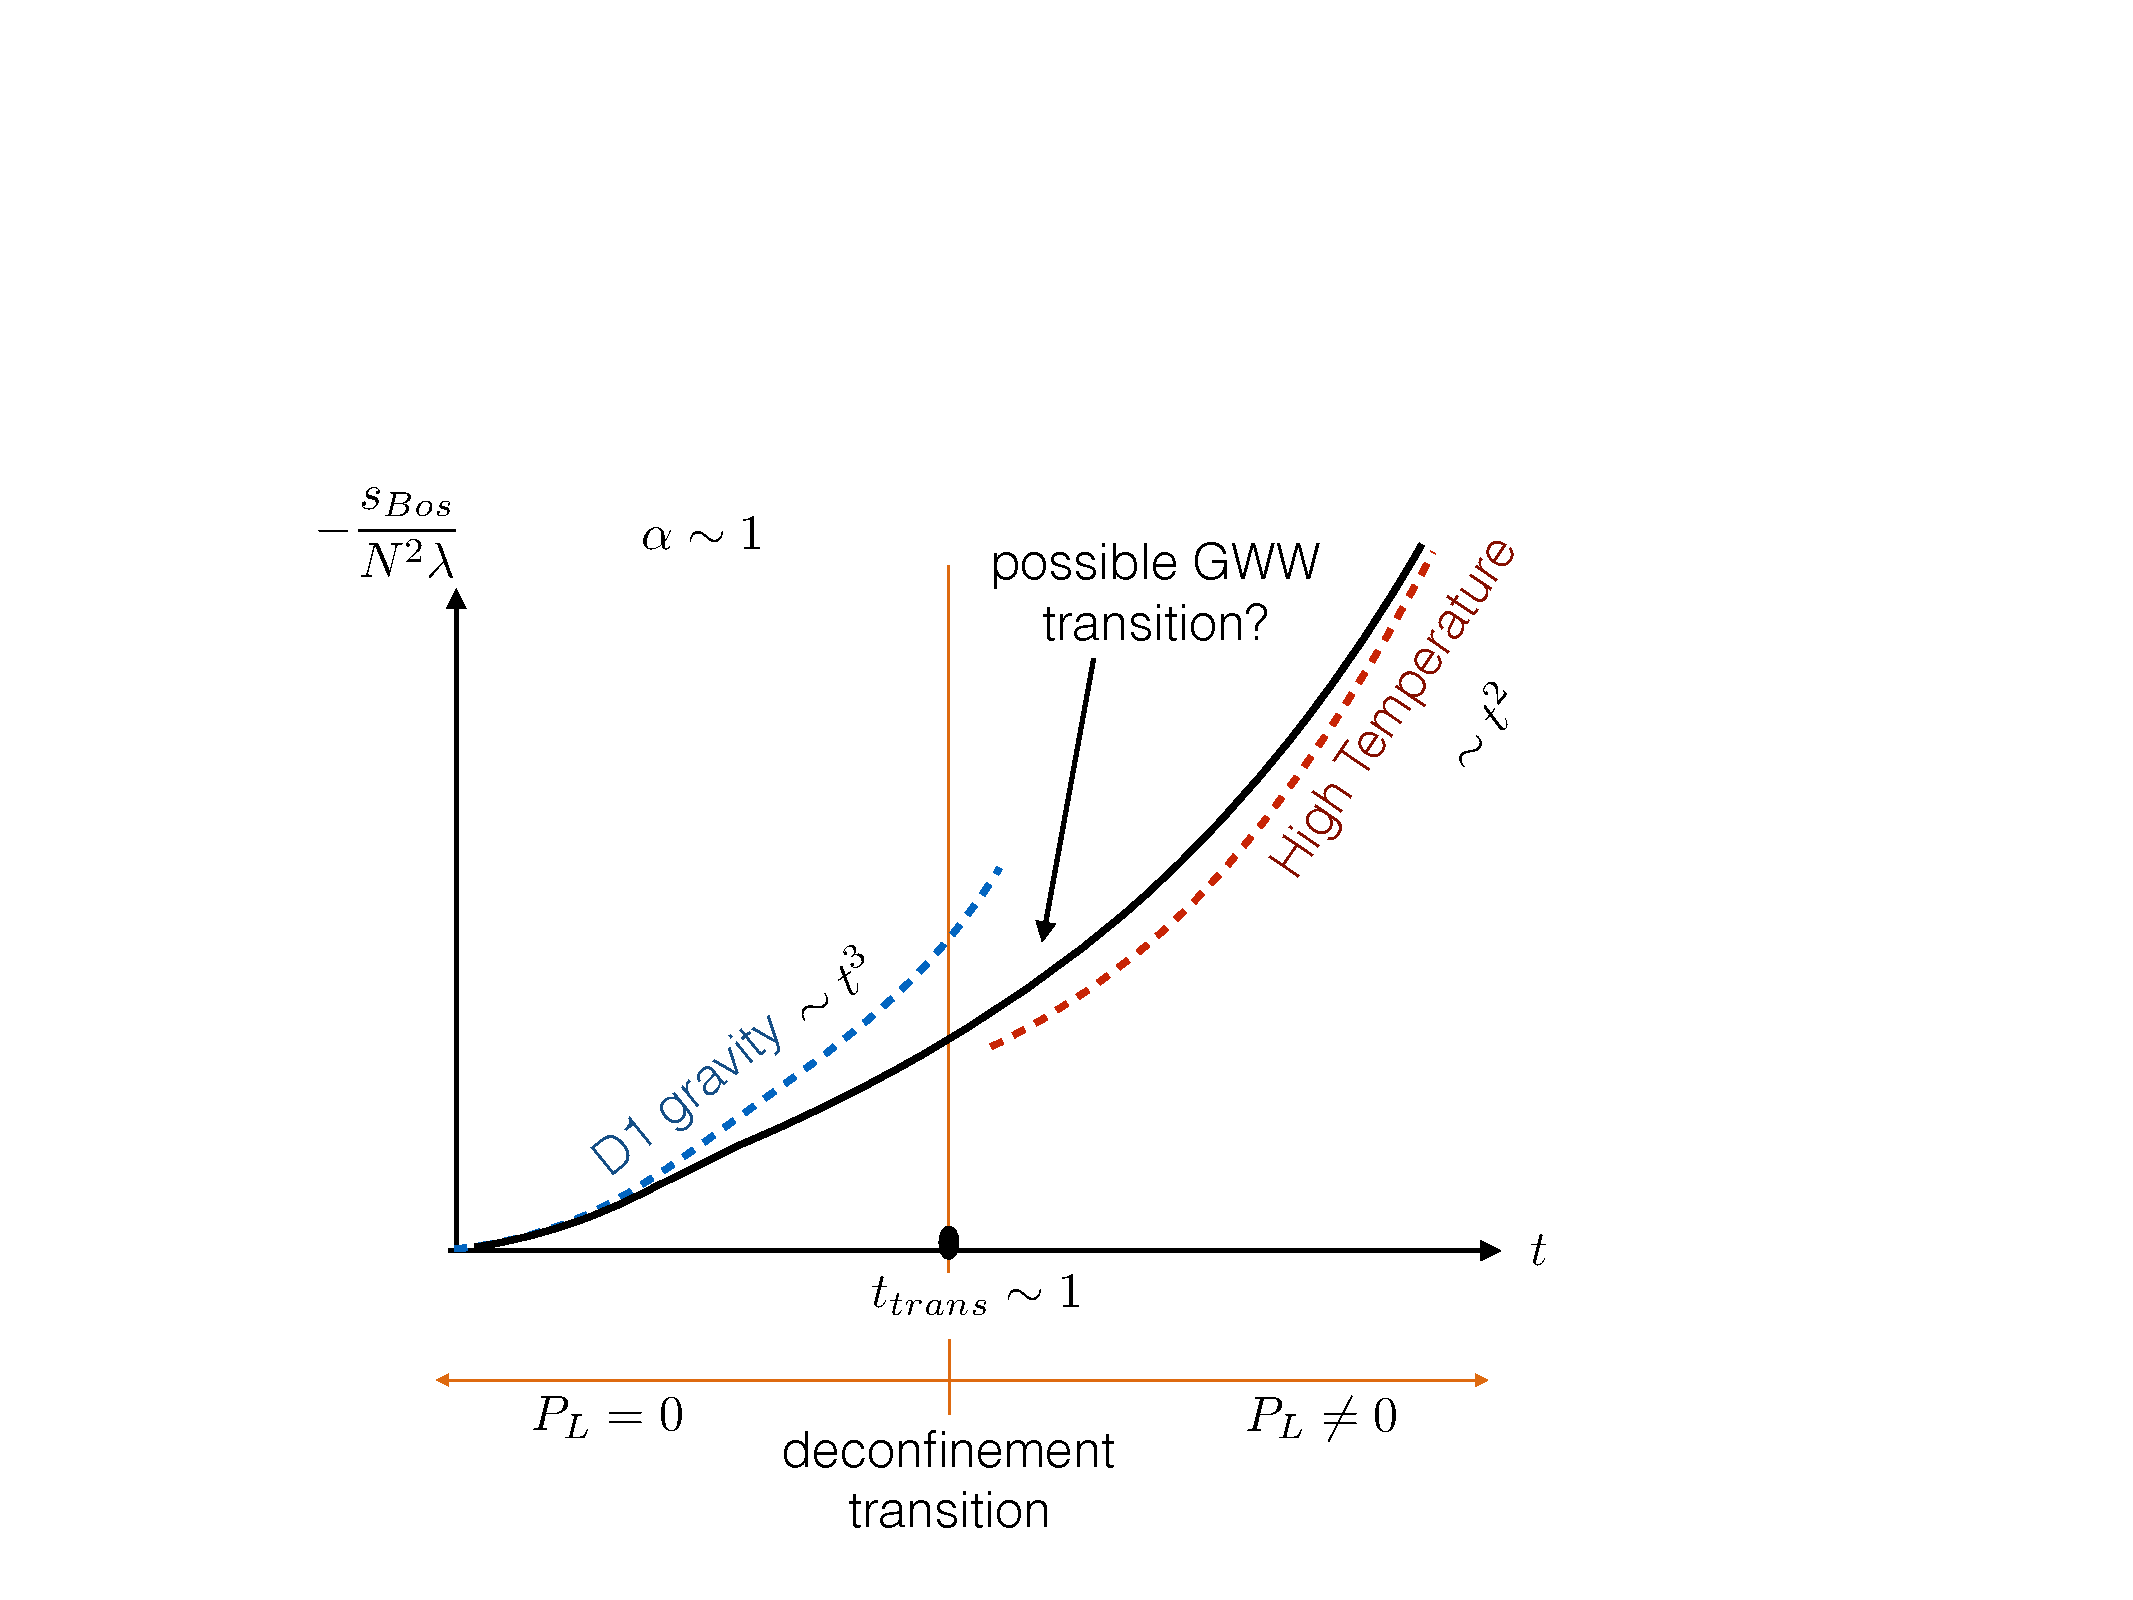
\includegraphics[height=6cm]{Figures/FigSummary1.pdf}
  \caption{\label{fig:summaryskew}Summary of the expected behavior of SYM on a skewed torus varying $t$ with fixed shape parameters $\al, \ga$.  As $t$ varies from high to low we pass from the small-volume $P_L \ne 0$ deconfined phase into the $P_L = 0$ confined gravity D1~phase.  For small \al (top-left plot) the low-$t$ behavior, including the phase transition, falls in the gravity regime.  Hence we see not only the D1~phase, but also the D0~phase and the first-order transition between them.  For large \al (top-right plot) the high-$t$ behavior including the phase transition to the $P_L = 0$ confined phase is described by the BQM reduction.}
\end{figure}

In our numerical analyses of the skewed SYM theory it will be convenient to fix $\al = r_L / r_{\beta}$ and vary $t = 1 / r_{\beta}$ to scan a `slice' of the $r_{\beta} \times r_L$ plane.
For any finite $\al$, at sufficiently high temperature $t \gg 1$ we will also be in the small-volume regime with $P_L \ne 0$.
As we decrease $t$, for \emph{any} finite \al we expect to go through a confinement phase transition associated to $P_L$, and for $t \ll 1$ eventually enter the gravity D1~phase with $P_L = 0$.
For large $\al \gg 1$ this will be the confinement transition described by BQM.
For small $\al \ll 1$ we expect to enter the gravity regime in the spatially deconfined D0~phase, and encounter the first-order dual Gregory--Laflamme transition to the D1~phase at the lower temperature $t = \al^2 / (\cgrav \sqrt{1 - \ga^2})$.
These expectations for large, small and intermediate \al are illustrated in figure~\ref{fig:summaryskew}.

%------------------------
\section{\label{sec:lattice}Lattice formulation}
Using ideas borrowed from topological field theory and orbifold constructions it has recently become possible to construct a four-dimensional lattice theory which retains exact supersymmetry at non-zero lattice spacing and produces $\cN = 4$ SYM in the continuum limit.
Noting that maximal SYM in any dimension can be thought of as a classical dimensional reduction of the $\cN = 1$ SYM in 10~dimensions, it follows that our theory of interest, maximal SYM in two dimensions, can be derived from a dimensional reduction of the four-dimensional $\cN = 4$ SYM theory.
Thus the approach we take here is to use the existing four-dimensional lattice construction of $\cN = 4$ SYM, and reduce this in two directions to obtain a two-dimensional lattice action for our desired two-dimensional SYM.

An interesting subtlety arises, namely that the four-dimensional lattice most naturally has a $A_4^*$ geometry rather than a hypercubic one.
When we reduce this lattice action, we obtain a discretization of two-dimensional SYM on a two-dimensional $A_2^*$ (triangular) lattice.
Taking the lattice to be periodic, with one direction having thermal (anti-periodic) fermion BCs and the other periodic BCs, we generate two-dimensional SYM on a 2-torus which is skewed, as the $A_2^*$ lattice basis vectors are not orthogonal.
However, as emphasized, this should be viewed as a virtue rather than a problem.
While there is no direct Lorentzian interpretation of this finite-volume `generalized' thermal ensemble, as discussed above there are holographic string theory predictions that can be tested, and that is the aim of this chapter.

We begin by considering the four-dimensional lattice discretization of topologically twisted $\cN = 4$ SYM.
We then outline how this is reduced to a two-dimensional system whose continuum limit will be the reduction of $\cN = 4$ SYM, giving maximal SYM in two dimensions.
Since the reduced lattice has a $A_2^*$ geometry, where we make one lattice direction into the thermal circle of length $\beta$ and the other into the spatial circle of length $L$, the continuum limit will be two-dimensional SYM living on a skewed torus.
The skewing parameter is then determined from the $A_2^*$ lattice geometry to be $\ga = -1 / 2$.
In appendix~\ref{app:scalar} we provide a detailed discussion of the reduction of a four-dimensional $A_4^*$ lattice theory to the two-dimensional $A_2^*$ lattice for a simpler scalar field theory.

%------------------------
\subsection{\label{sec:lattice_4d}Four-dimensional twisted lattice $\cN = 4$ SYM}
In this section, we summarize the important features of this four-dimensional lattice theory before proceeding to its dimensional reduction.
The trick to preserving supercharges in a lattice theory is to discretize a topologically twisted formulation of the underlying supersymmetric theory.\footnote{In the case of gauge theories these lattice formulations were first derived using ideas from orbifolding and deconstruction~\cite{Cohen:2003xe, Cohen:2003qw, Kaplan:2005ta}.}
In the case of $\cN = 4$ SYM, the twisted construction treats the four-component gauge field and the six massless adjoint scalars of the theory as a five-component complexified gauge field
\begin{equation}
  \label{complexification}
  \cA_a \equiv A_a + iB_a,
\end{equation}
where the roman index `$a$' runs from 1 to 5.
The four Majorana fermions of the theory are decomposed into $\chi_{ab} = -\chi_{ba}$, $\psi_a$ and $\eta$.
The analogous decomposition of the sixteen supercharges provides a twisted-scalar \cQ corresponding to $\eta$, which is nilpotent, $\cQ^2 = 0$.
The complexified gauge field leads to complexified field strengths
\begin{align}
  \cF_{ab} & \equiv [\cD_a, \cD_b] &
  \cFbar_{ab} & \equiv [\cDbar_a, \cDbar_b],
\end{align}
where the corresponding complexified covariant derivatives are
\begin{align}
  \cD_a & = \partial_a + \cA_a &
  \cDbar_a & = \partial_a + \cAb_a.
\end{align}
Using these ingredients we can express the usual $\cN = 4$ action as a sum of $\cQ$-exact and $\cQ$-closed terms,
\begin{equation}
  \label{eq:contSYM}
  \begin{split}
    S & = \frac{N}{4\lam_4} \cQ \int d^4 x \ \Tr{\chi_{ab}\cF_{ab} + \eta [\cDbar_a, \cD_a] - \frac{1}{2}\eta d} + S_{\text{cl}} \\
    S_{\text{cl}} & = -\frac{N}{16\lam_4} \int d^4 x \ \Tr{\epsilon_{mnpqr} \chi_{qr} \cDbar_p \chi_{mn}},
  \end{split}
\end{equation}
where $\lam_4 = g^2 N$ is the usual 't~Hooft coupling and we implicitly sum over repeated indices.
Here $x_{\al}$ are the usual canonical flat-space coordinates with \al running from 1 to 4.
The action of the scalar supersymmetry charge \cQ is
\begin{align}
  & \cQ\; \cA_a = \psi_a         & & \cQ\; \psi_a = 0 \cr
  & \cQ\; \chi_{ab} = -\cFbar_{ab} & & \cQ\; \cAb_a = 0 \\
  & \cQ\; \eta = d               & & \cQ\; d = 0,     \nn
\end{align}
where $d$ is a bosonic auxiliary field with equation of motion $d = \left[\cDbar_a, \cD_a\right]$.
Since $\cQ^2 = 0$ the $\cQ$-exact part of the action is clearly supersymmetric, while \cQ acting on the $\cQ$-closed term vanishes due to a Bianchi identity.
The other fifteen supercharges are twisted into a 1-form $\cQ_a$ and antisymmetric 2-form $\cQ_{ab}$.

This continuum action can be discretized while preserving the single \cQ supersymmetry as described in refs.~\cite{Kaplan:2005ta, Catterall:2007kn, Damgaard:2008pa, Catterall:2014vka}.
This discretization procedure dictates how the continuum fields are placed on the lattice, how derivatives are replaced by lattice difference operators and even the structure of the underlying lattice itself.
Specifically, we must employ the $A_4^*$ lattice whose five basis vectors symmetrically span the four spacetime dimensions.
This lattice is a natural generalization of the two-dimensional triangular ($A_2^*$) lattice to four dimensions.
It possesses five equivalent basis vectors corresponding to the vectors from the center of an equilateral four-simplex out to its five vertices.
It has a high $S_5$ point group symmetry with the dimensions of its low lying irreducible representations matching those of the continuum twisted SO(4) rotation group.
Ref.~\cite{Catterall:2014mha} shows that the combination of the \cQ supersymmetry, lattice gauge invariance and the $S_5$ global symmetry suffices to ensure that no new relevant operators are generated by quantum corrections.
Assuming non-perturbative effects such as instantons preserve the lattice moduli space, only a single marginal coupling may need to be tuned to obtain $\cN = 4$ SYM in the continuum limit.

The resultant lattice action takes the form
\begin{align}
  S_0 & = \frac{N}{4\lalat} \sum_{\vn} \Tr{\cQ \left(\chi_{ab}(\vn)\cD_a^{(+)}\cU_b(\vn) + \eta(\vn) \cDbar_a^{(-)}\cU_a(\vn) - \frac{1}{2}\eta(\vn) d(\vn) \right)} + S_{\text{cl}} \\
  S_{\text{cl}} & = -\frac{N}{16\lalat} \sum_{\vn} \Tr{\epsilon_{abcde} \chi_{de}(\vn + \hatbmu_a + \hatbmu_b + \hatbmu_c) \cDbar^{(-)}_{c} \chi_{ab}(\vn + \hatbmu_c)},
\end{align}
where the lattice difference operators appearing in the above expression are given in refs.~\cite{Catterall:2007kn, Damgaard:2008pa} and generically take the form of shifted commutators.
For example,
\begin{equation}
  \cD_a^{(+)}\cU_b(\vn) = \cU_a(\vn)\cU_b(\vn + a) - \cU_b(\vn)\cU_a(\vn + b).
\end{equation}
Remarkably the $\cQ$-closed term is still lattice supersymmetric due to the existence of an exact lattice Bianchi identity,
\begin{equation}
  \epsilon_{abcde} \cDbar^{(-)}_c \cFbar_{ab}(\vn + \hat{\mu}_c) = 0.
\end{equation}
Integrating out the auxiliary field $d$ yields
\begin{equation}
  \label{eq:lat_act}
  \begin{split}
    S_0 & = \frac{N}{4\lalat} \sum_{\vn} \text{Tr}\left[-\cFbar_{ab}(\vn) \cF_{ab}(\vn) + \frac{1}{2}\left(\cDbar_a^{(-)}\cU_a(\vn)\right)^2 \right. \\
        & \hspace{5 cm} \left. - \chi_{ab}(\vn) \cD^{(+)}_{[a}\psi_{b]}(\vn) - \eta(\vn) \cDbar^{(-)}_a\psi_a(\vn)\right] + S_{\text{cl}}.
  \end{split}
\end{equation}
The lattice sites in the canonical flat-space coordinates $x^{\al}$ of eq.~\eqref{eq:contSYM} are arranged as the $A_4^*$ lattice with positions $x^{\al} = \Delta\, \vn^{\nu} e_{(\nu)}^{\al}$ for $\vn \in \mathbb{Z}^4$.
This discretization is analogous to that discussed explicitly for the scalar theory example in appendix~\ref{app:scalar}.
As discussed following eq.~\eqref{eq:4dact1}, the resulting continuum action~\eqref{eq:contSYM} has a coupling related to the lattice coupling as $\lam_4 = \lalat / \sqrt{5}$~\cite{Kaplan:2005ta, Catterall:2014vka}.

The presence of exact lattice supersymmetry allows us to derive an exact expression for the renormalized bosonic action density, which gives the derivative of the partition function with respect to the coupling as in eq.~\eqref{bosonicaction}.
We find
\begin{equation}
  \label{eq:subtraction}
  \vev{s_{\text{Bos}}} = \left( \frac{\vev{S_B^{\text{lat}}}}{V} - \frac{9N^2}{2} \right)
\end{equation}
where $V$ denotes the number of lattice sites and $S_B^{\text{lat}}$ corresponds to the bosonic terms in the lattice action.
This definition of the continuum renormalized $\vev{s_{\text{Bos}}}$ has the property that it vanishes as a consequence of the exact lattice supersymmetry if periodic (non-thermal) BCs are used.

In practice, to stabilize the SU($N$) flat directions of the theory we add to $S_0$ a soft-supersymmetry-breaking scalar potential
\begin{equation}
  \label{eq:single_trace}
  S_{\text{soft}} = \frac{N}{4\lalat} \mu^2 \sum_{\vn,\ a} \Tr{\bigg(\cUbar_a(\vn) \cU_a(\vn) - \Ibb_N\bigg)^2}
\end{equation}
with tunable parameter $\mu$.
In the dimensionally reduced system, this term is particularly important at low temperatures where the flat directions lead to thermal instabilities~\cite{Catterall:2009xn}.
This single-trace scalar potential differs from the double-trace operator used in previous investigations~\cite{Catterall:2014vka, Schaich:2014pda, Catterall:2014vga} and 
constrains each eigenvalue of $\cUbar_a \cU_a$ individually, rather than only the trace as a whole.
Exact supersymmetry at $\mu = 0$ ensures that all $\cQ$-breaking counterterms vanish as some power of $\mu$.

The complexification of the gauge field in eq.~\eqref{complexification} leads to an enlarged U($N$) = SU($N$) $\otimes$ U(1) gauge invariance.
In the continuum, the U(1) sector decouples from observables in the SU($N$) sector, but this is not automatic at non-zero lattice spacing~\cite{Catterall:2014vka, Schaich:2014pda, Catterall:2014vga}.
To regulate additional flat directions in the U(1) sector, we truncate the theory to remove the U(1) modes from $\cU_a$, making them elements of the group SL($N, \Cbb$) rather than the algebra $\glN$.
In order to maintain SU($N$) gauge invariance, it is necessary to keep the fermions in $\glN$, explicitly breaking the lattice supersymmetry that would have related $\cU_a$ to $\psi_a$.
However, by representing the truncated gauge links as $\cU_b = e^{iga \cA_b}$, we can argue that the continuum supersymmetry relating $\cA_a$ and $\psi_a$ is approximately realized in the large-$N$ limit even at non-zero lattice spacing.
This follows from fixing the 't~Hooft coupling $\lalat = g^2 N$ as $N \to \infty$, implying $g^2 \to 0$.
Then expanding the exponential produces the desired $\cU_b = \Ibb_N + iga\cA_b$ up to $\cO(ga)$ corrections that vanish as $N \to \infty$ even at non-zero lattice spacing $a$.
Empirically, when we measure would-be supersymmetric Ward identities we find that they are satisfied up to small (at most percent-level) deviations, and those deviations decrease $\propto 1 / N^2$ as $N$ increases.
(Figure~\ref{fig:ward} in the appendix shows some representative results.)
Although the constant term in eq.~\eqref{eq:subtraction} is no longer exactly $9 / 2$, we expect only comparably small corrections to it and therefore continue to use eq.~\eqref{eq:subtraction} to define $s_{\text{Bos}}$.
Since our lower-dimensional studies all focus on holographic dualities in the large-$N$ limit, this truncated approach appears viable at least in fewer than four dimensions.

%------------------------
\subsection{\label{sec:lattice_2d}Two-dimensional twisted lattice $\cN = (8, 8)$ SYM}
Our interest is in two-dimensional maximal SYM on a 2-torus with thermal (anti-periodic) fermion BCs on one cycle and periodic BCs on the other.
This two-dimensional maximal SYM is given by the dimensional reduction of the four-dimensional $\cN = 4$ theory.
Hence to obtain this two-dimensional theory on a 2-torus we simply consider the above four-dimensional lattice discretization of the $\cN = 4$ theory, taken on $N_x \times 1 \times 1 \times N_t$ lattices with periodic BCs in the reduced directions, corresponding to naive dimensional reduction.
The gauge fields associated with the reduced directions now transform as site fields $\varphi_i(\vn)$ and are naturally interpreted as the scalar fields arising from dimensional reduction.
Their fermionic superpartners, now also site fields, correspond to additional exact lattice supersymmetries~\cite{Damgaard:2008pa}.

Exactly as for the scalar example discussed in appendix~\ref{app:scalar}, such a reduction results in a continuum theory in two-dimensional flat space where the lattice geometry is that of $A_2^*$.
We take appropriate periodicity conditions on the extended lattice directions, $\vn \sim \vn + (0, 0, 0, N_t)$ with anti-periodic fermions and $\vn \sim \vn + (N_x, 0, 0, 0)$ with periodic fermions, thus generating the 2-torus.
Since the two-dimensional lattice has $A_2^*$ geometry the 2-torus we generate is not rectangular but skewed, with $\ga = \frac{\tilde{\ve}_1 \cdot \tilde{\ve}_2}{|\tilde{\ve}_1| |\tilde{\ve}_2|} = -1 / 2$.
The lengths of the two cycles are then
\begin{align}
  \beta & = a_2 \, N_t &
  L & = a_2 \, N_x,
\end{align}
where we see from appendix~\ref{app:scalar} that the two-dimensional lattice spacing is $a_2 = \Delta \sqrt{2 / 3}$.
Similarly, the two-dimensional continuum gauge coupling is
\begin{equation}
  \lam = \frac{\lalat}{\Delta^2 \sqrt{3}} = \frac{\lam_4}{\Delta^2} \sqrt{\frac{5}{3}},
\end{equation}
where the second equality from eq.~\eqref{eq:KKcoupling} considers the coupling as arising from an appropriate Kaluza--Klein reduction of the continuum four-dimensional $\cN = 4$ theory.
Thus in terms of our dimensionless couplings our lattice action corresponds to two-dimensional $\cN = (8, 8)$ SYM on a skewed torus with $\ga = -1 / 2$ and
\begin{align}
  r_{\beta} & = \beta \sqrt{\lam} = N_t \sqrt{\frac{2\lalat}{3\sqrt{3}}} &
  r_L & = L \sqrt{\lam} = N_x \sqrt{\frac{2\lalat}{3\sqrt{3}}},
\end{align}
which, being dimensionless, are independent of the scale $\Delta$ as they should be.
Noting that in two dimensions the continuum SYM is super-renormalizable, we do not expect any renormalization of the classical geometry of this 2-torus.

Finally, for the dimensionally reduced lattice theory to correctly reproduce the physics of the continuum theory requires $\Tr{\varphi_i} \approx N$ in the reduced directions $i = y$ and $z$.
This corresponds to broken center symmetries in those two directions.
We ensure this by adding another soft-$\cQ$-breaking term to the lattice action,
\begin{equation}
  \label{eq:center}
  S_{\text{center}} = -\frac{N}{4\lalat} c_W^2 \sum_{\vn,\ i = y, z} 2\text{ReTr}\bigg[\varphi_i(\vn) + \varphi_i^{-1}(\vn)\bigg].
\end{equation}
This is gauge invariant since $\varphi_i(\vn)$ transform as site fields.
In this work we use either $c_W^2 = \mu^2$ or $c_W^2 = 0$, again extrapolating $\mu^2 \to 0$ in the former case.

%------------------------
\subsection{\label{sec:torusgeom}Torus geometries}
The geometry of our tori is determined by the skewing parameter $\ga = -1 / 2$ set by our lattice discretization, and by the aspect ratio $\al = r_L / r_{\beta} = N_x / N_t$, where $N_x$ and $N_t$ are respectively the numbers of lattice points generating the spatial and temporal cycles.
As mentioned earlier, we will typically discuss results specifying the torus with the skewing $\ga = -1 / 2$, but this parameterization may represent a modular parameter outside the fundamental domain.
Here we review the geometries we will consider and their fundamental parameterization.
In particular, while we use a skewed lattice, some of our geometries, in fact, are those of rectangular tori when mapped to the fundamental domain.


\begin{table}[htbp]
  \centering
  \renewcommand\arraystretch{1.2}   % Increase the height of each row
  \addtolength{\tabcolsep}{1 pt}    % Increase separation between columns
  \begin{tabular}{c|c|c|c|c|c}
    \al     & $N_x \times N_t$            & Modular Transformation                                            & $\left(\al', \ga'\right)$                                & $t' / t$             &             \\
    \hline
    $1 / 2$ &  $6\times 12$, $8\times 16$ & $\vec{\beta}' = \vec{\beta} + \vec{L}$, $\vec{L}' = \vec{L}$      & $\left(\frac{1}{\sqrt{3}}, 0\right)$                     & $\frac{2}{\sqrt{3}}$ & Rectangular \\
    1       & $16\times 16$, $8\times 8$  & ---                                                               & ---                                                      & ---                  & Skewed      \\
    $3 / 2$ & $12\times 8$, $18\times 12$ & ---                                                               & ---                                                      & ---                  & Skewed      \\
    2       & $16\times 8$, $24\times 12$ & ---                                                               & ---                                                      & ---                  & Skewed      \\
    $8 / 3$ & $16\times 6$, $24\times 9$  & $\vec{L}' = \vec{L} + 2\vec{\beta}$, $\vec{\beta}' = \vec{\beta}$ & $\left(\frac{2\sqrt{13}}{3}, \frac{1}{\sqrt{13}}\right)$ & 1                    & Skewed      \\
    4       & $16\times 4$, $24\times 6$  & as above                                                          & $\left(2\sqrt{3}, 0\right)$                              & 1                    & Rectangular \\
    6       & $24\times 4$                & as above                                                          & $\left(2\sqrt{7}, -\frac{1}{2\sqrt{7}}\right)$           & 1                    & Skewed      \\
    8       & $32\times 4$                & $\vec{L}' = \vec{L} + 4\vec{\beta}$, $\vec{\beta}' = \vec{\beta}$ & $\left(4\sqrt{3}, 0\right)$                              & 1                    & Rectangular \\
  \end{tabular}
  \caption{\label{tab:tori}The lattice geometries we numerically analyze.  Our lattice discretization naturally picks $\ga = -1 / 2$, and by varying the spatial and temporal lattice extents $N_x$ and $N_t$ we generate tori with different aspect ratios $\al$.  When these $(\al, \ga)$ denote a torus with modular parameter $\uptau$ outside the fundamental domain, we give an appropriate modular transformation (as in eq.~\eqref{eq:SLtransform}) so that the equivalent $(\al', \ga')$ lie within it.  We also give the relation between the temperatures $t' / t$.  The last column states whether the torus, viewed from the fundamental domain, is skewed or rectangular.}
\end{table}

\begin{figure}[htbp]
  \centering
  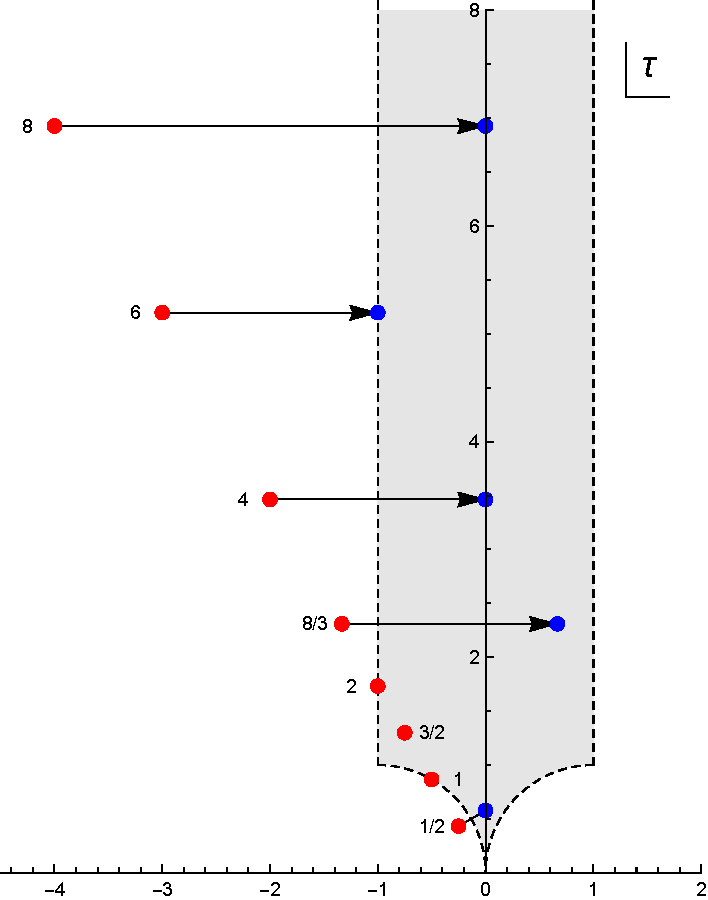
\includegraphics[height=9cm]{Figures/tauplot.pdf}
  \caption{\label{fig:tauplot}Plot of the torus modular parameters $\uptau$ in the complex plane for the aspect ratios \al we numerically analyze.  The red points are for the $\ga = -1 / 2$ of our lattice discretization, with the corresponding \al written next to them.  The fundamental domain is shaded, and when a point lies outside it the equivalent $\uptau'$ lying within it is shown as a blue point.}
\end{figure}

In table~\ref{tab:tori} we list the lattice sizes $N_x \times N_t$ we numerically analyze, together with their shape parameter \al for skewing $\ga = -1 / 2$.
When the corresponding modular parameter $\uptau$ doesn't fall in the fundamental domain we give a modular transformation to an equivalent representation with shape parameters $\al', \ga'$, and note whether the fundamental representation is rectangular or skewed.
We also give $t' / t$, the ratio between the dimensionless temperature in the new representation to that of the original.
In the corresponding figure~\ref{fig:tauplot} we plot the complex $\uptau$ parameters for the various tori in the natural representation where $\ga = -1 / 2$, and in the cases where these lie outside the fundamental domain we draw an equivalent $\uptau'$ contained in it.

%------------------------
\section{\label{sec:results}Numerical results}
We now discuss our numerical results obtained using the lattice formulation described above.
Before studying the low-temperature regime relevant for supergravity, we first consider the high-temperature, small-volume limit and then the phase structure of the theory.

%------------------------
\subsection{High-temperature limit}
Fixing the shape of the torus, with constant \al for $\ga = -1 / 2$, we vary $t \to \infty$.
Following our earlier discussion in section~\ref{sec:summaryskew}, this is the high-temperature, small-volume limit where we expect the theory to be spatially deconfined with $P_{\beta}, P_L \ne 0$, and to have bosonic action density~\eqref{eq:HT}.

\begin{figure}[tbp]
  \centering
  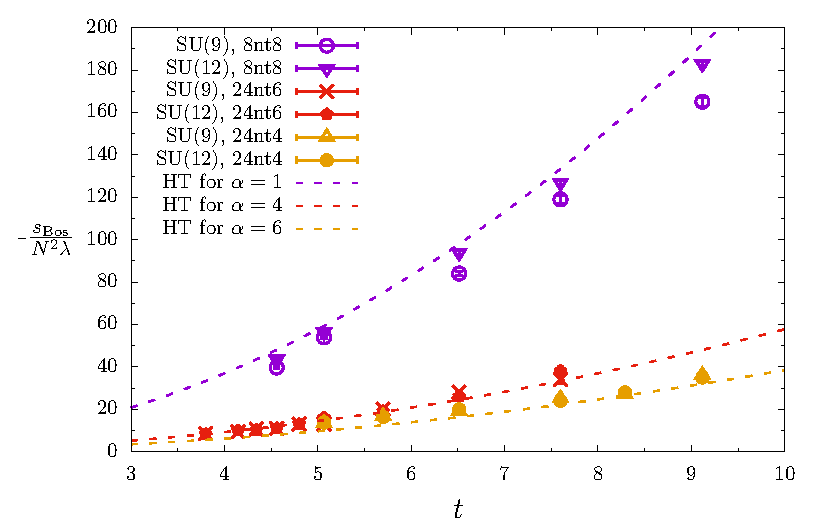
\includegraphics[height=9cm]{Figures/highT.pdf}
  \caption{\label{fig:highT}Bosonic action density versus dimensionless temperature $t$ for three aspect ratios $\al = 1$, 4 and 6 (from top to bottom), considering gauge groups SU(9) and SU(12).  The temperature range probed here corresponds to the high-temperature, small-volume limit, and the prediction~\protect\eqref{eq:HT} for the behavior is given by the dashed curves marked HT.}
\end{figure}

We investigate three different aspect ratios ($\al = 1$, 4 and 6) in the high-temperature regime and plot the bosonic action density in figure~\ref{fig:highT}.
Qualitative agreement is seen both in the power of $t$ and the $\al$-dependent coefficient, providing a test of the dimensional reduction that relates the lattice coupling \lalat to the dimensionless continuum parameters $r_L$ and $r_{\beta}$.

\begin{figure}[tbp]
  \centering
  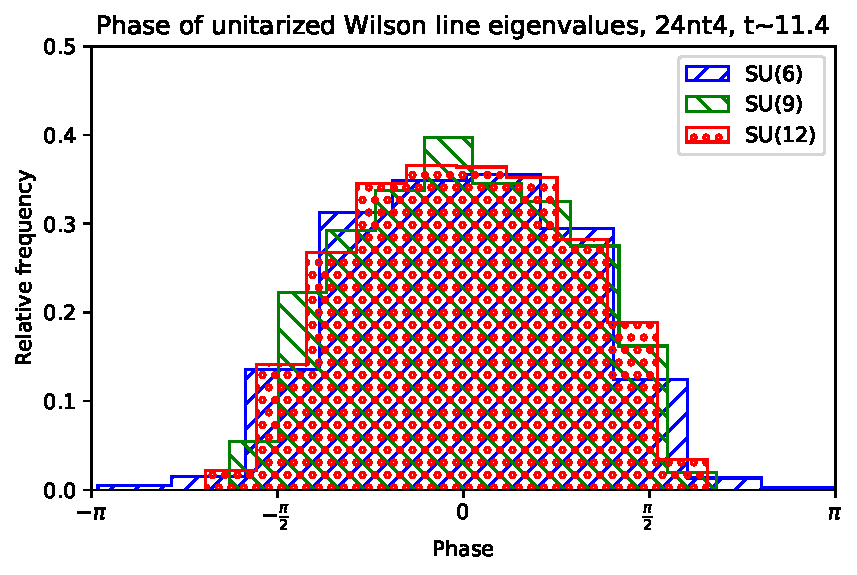
\includegraphics[height=9cm]{Figures/WLeig-highT.pdf}
  \caption{\label{fig:WLeig-highT}Distributions of the phases of the $N$ eigenvalues of spatial Wilson line on $24\times 4$ lattices at a high temperature $t \approx 11.4$, for SU($N$) gauge groups with $N = 6$, 9 and 12.  The phases are measured relative to the average phase of each Wilson line.  The compact distributions correspond to broken $Z_N$ center symmetry in the spatially deconfined high-temperature phase.}
\end{figure}

It is important to note that the Wilson loop we study has scalar contributions as well and it is no longer unitary and 
hence we cannot talk of an eigenvalue distribution on a circle.
However, we do a polar decomposition and consider only gauge fields and hence the unitarized Wilson loop. 

In figure~\ref{fig:WLeig-highT} we show distributions of the phases of the $N$ eigenvalues of spatial Wilson lines $\cP e^{i\oint_L A}$ on $24\times 4$ lattices ($\al = 6$) at a high temperature $t \approx 11.4$, for SU($N$) gauge groups with $N = 6$, 9 and 12.
The phases are measured relative to the average phase of each Wilson line.
In order to compute the usual Wilson lines from the complexified gauge links $\cU_a$ of the lattice formulation, we use a polar decomposition $\cU_a = H_a \cdot U_a$ to separate each link into a positive-semidefinite hermitian matrix $H_a$ (containing the scalar fields) and a unitary matrix $U_a$ corresponding to the gauge field.
To compute the Wilson lines we simply multiply the unitary matrices, $\prod_{i = 1}^{N_x} U_x(x_i, \tau)$ and $\prod_{i = 1}^{N_t} U_t(x, \tau_i)$.
We construct $P_L$ and $P_{\beta}$ by taking the trace (normalized to 1), averaging over lattice sites in the temporal and spatial direction (respectively), and then computing the ensemble average of the magnitude.
The expectation that $P_L \sim 1$ implies we should expect a localized distribution of the phases of the spatial Wilson line eigenvalues, which is consistent with the results in figure~\ref{fig:WLeig-highT}.
The distributions show little dependence on $N$, though the $N = 6$ case has a few outliers with large fluctuations from the average phase.
As $t$ decreases we expect a transition with $P_L \to 0$, with the eigenvalue distribution spreading over the angular circle and becoming uniform on it.
For $t \lesssim 9$ we do indeed see the distributions spread out over the full angular period, as we discuss in more detail below. 

%------------------------
\subsection{Phase structure of the SYM theory}
\begin{figure}[tbp]
  \centering
  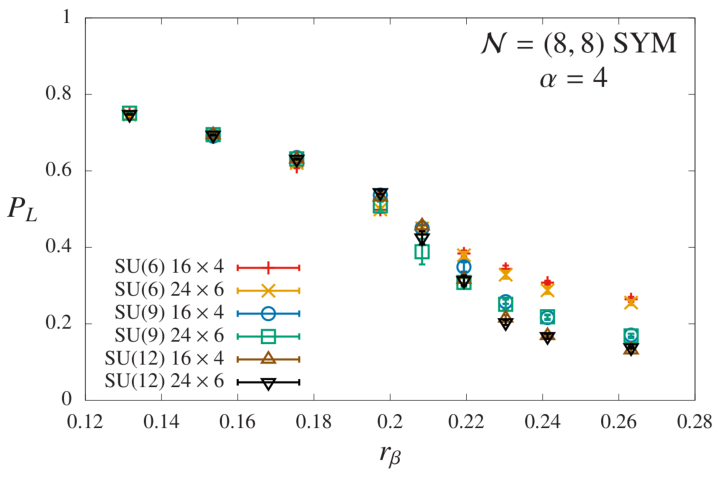
\includegraphics[height=9cm]{Figures/lines_alpha4.pdf}
  \caption{\label{fig:lines_alpha4}Spatial Wilson loop magnitude vs.~inverse dimensionless temperature $r_{\beta} = 1 / t$ for SU($N$) gauge groups with $N = 6$, 9 and 12 on $16\times 4$ and $24\times 6$ lattices (aspect ratio $\al = 4$).}
\end{figure}

\begin{figure}[tbp]
  \centering
  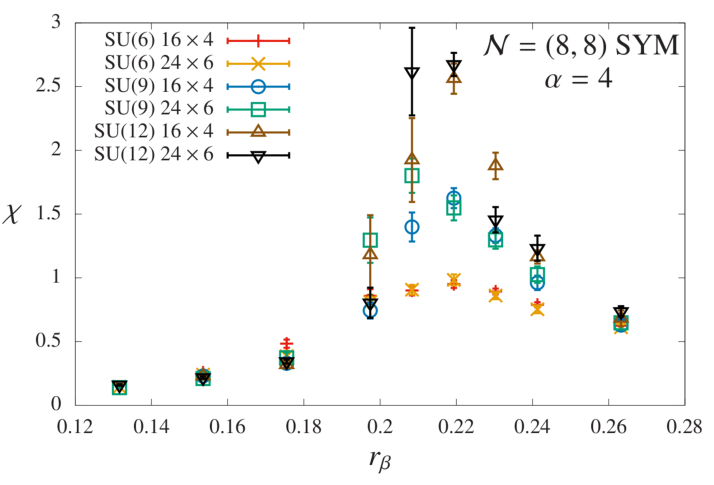
\includegraphics[height=9cm]{Figures/sus_alpha4.pdf}
  \caption{\label{fig:sus_alpha4} The corresponding peak of the susceptibility of the transition strengthens as $N$ increases, without showing visible sensitivity to the lattice size for this $\alpha$. }
\end{figure}

We have explored the phase structure of the SYM theory by scanning in $t = 1 / r_{\beta}$ for fixed aspect ratio $\al = r_L / r_{\beta}$.
From our previous discussion, we expect the theory to be thermally deconfined, but to have an interesting phase structure associated with spatial confinement.
Our numerical results for the temporal Wilson loop magnitude $P_{\beta}$ appear consistent with the theory being thermally deconfined.
We now focus on the spatial Wilson line and order parameter $P_L$.

In figure~\ref{fig:lines_alpha4} we show the jackknife average magnitude of the Wilson line $P_L$ vs.~$r_{\beta}$ for $\al = 4$, along with the corresponding susceptibility in figure~\ref{fig:sus_alpha4}. 
\begin{equation}
  \chi = \vev{\left| \Tr{\cP e^{i\oint_L A}} \right|^2} - \vev{\left| \Tr{\cP e^{i\oint_L A}} \right|}^2.
\end{equation}
The results indicate a large-$N$ transition at $t_c = 4.6(2)$ separating a spatially deconfined phase with $P_L \ne 0$ at small $r_{\beta}$ (high temperatures) from a spatially confined phase at large $r_{\beta}$ (low temperatures) where $P_L \to 0$ as $N \to \infty$.
This transition strengthens with larger $N$, as can be seen, most clearly from the $N$ dependence of the points at large $r_{\beta}$.
The consistent results for $16\times 4$ and $24\times 6$ lattices indicate that discretization effects are small.
As discussed in section~\ref{sec:torusgeom} (table~\ref{tab:tori}), the geometry $\al = 4$ for $\ga = -1 / 2$ is equivalent to a rectangular ($\ga' = 0$) torus with $\al' = 2\sqrt{3}$ and $r_{\beta}' = r_{\beta}$.

\begin{figure}[tbp]
  \centering
  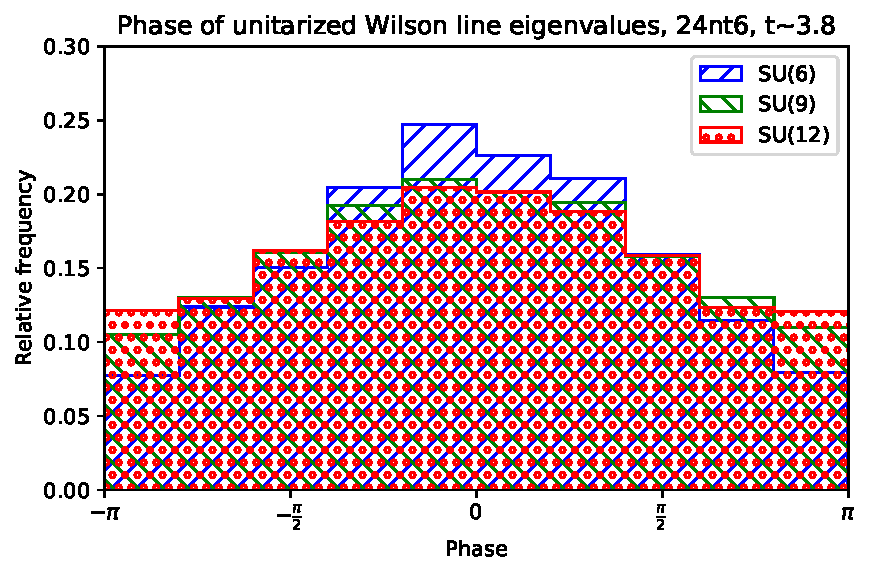
\includegraphics[height=9cm]{Figures/WLeig-lowT.pdf}
  \caption{\label{fig:WLeig-lowT}Distributions of Wilson line eigenvalue phases, as in figure~\protect{\ref{fig:WLeig-highT}}, for $24\times 6$ lattices at a lower temperature $t \approx 3.8$.  The distributions are no longer compact, and instead spread throughout the angular period, as expected from the black-string phase of the gravity dual.}
\end{figure}

In figure~\ref{fig:WLeig-lowT} we plot distributions of the spatial Wilson line eigenvalue phases, following the same procedure as described for figure~\ref{fig:WLeig-highT} while considering a lower temperature $t \approx 3.8$ on $24\times 6$ lattices ($\al = 4$).
Since $t < t_c$ we expect to be in a spatially confined phase, with $P_L \to 0$ and correspondingly a uniform density of eigenvalue phases on the angular circle.
As expected, we do observe these phases spreading out around the angular period in figure~\ref{fig:WLeig-lowT}, and the distribution becomes more uniform as $N$ increases.
This contrasts with the localized distributions in figure~\ref{fig:WLeig-highT} for the high-temperature spatially deconfined phase.

\begin{figure}[tbp]
  \centering
  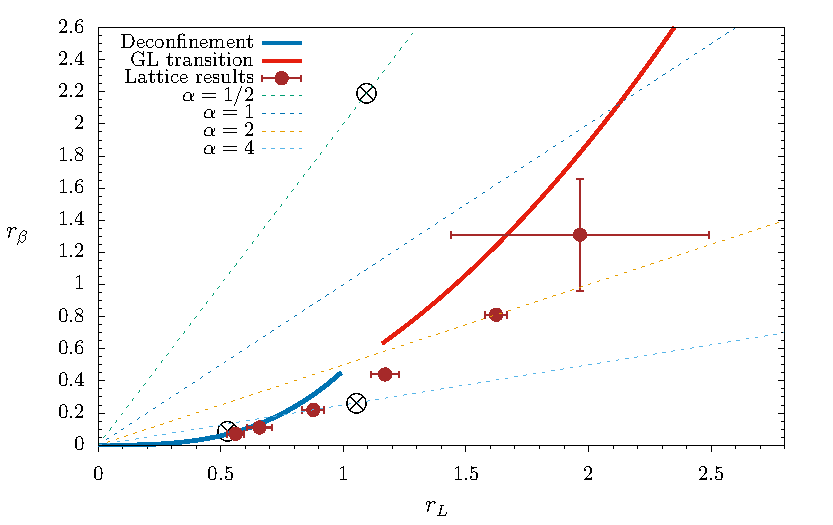
\includegraphics[height=9cm]{Figures/crit.pdf}
  \caption{\label{fig:crit}The points show the $(r_L, r_{\beta})$ positions of the spatial deconfinement transitions for six aspect ratios $8 \geq \al \geq 3 / 2$ (from left to right), determined from our lattice calculations of the Wilson line susceptibility (cf.\ figure~\protect\ref{fig:sus_alpha4}).  The three $\bigotimes$ symbols mark the ensembles whose Wilson line eigenvalue phase distributions we show in figures~\protect\ref{fig:WLeig-highT}, \protect\ref{fig:WLeig-lowT} and \protect\ref{fig:WLeig-al05} (from bottom to top; the point for figure~\protect\ref{fig:WLeig-al2} lies outside the range of the plot).  The solid lines show the expected transitions sketched in figure~\protect\ref{fig:summaryrect}: the BQM deconfinement transition at high temperature and the low-temperature Gregory--Laflamme transition.  The dashed lines indicate constant aspect ratios $1 / 2 \leq \al \leq 4$ from top to bottom.}
\end{figure}

Using the Wilson line susceptibility (cf.\ figure~\ref{fig:lines_alpha4}) we have mapped the position of the spatial deconfinement phase transition as a function of \al for our $\ga = -1 / 2$.
In figure~\ref{fig:crit} we plot our results on the $r_L$--$r_{\beta}$ plane and compare them with the expected transitions sketched in figure~\ref{fig:summaryrect}.
For $\al \gtrsim 4$ we find the transition occurs at high temperatures $r_{\beta} \ll 1$, and nicely agrees with the deconfinement transition behavior predicted by the high-temperature BQM limit we discussed in section~\ref{sec:smallcircle}.
Unfortunately, our uncertainties increase significantly as we approach transitions occurring at lower temperatures (and smaller $\al$) where we expect the dual gravitational prediction~\eqref{eq:skewtransition} to apply.
Given their large uncertainties, our results are certainly consistent with the low-temperature behavior predicted by holography, though we are not yet able to test this prediction with great accuracy.
As figure~\ref{fig:lines_sus_alpha4} shows, the Wilson line susceptibility $\chi$ is a noisy observable, which forces us to ignore the statistical uncertainties in our results and simply identify the transition as the $r_{\beta}$ corresponding to the largest central value of $\chi$.
The uncertainties shown in figure~\ref{fig:crit} then indicate the neighboring $r_{\beta}$ with smaller $\chi$.
Even this simplified procedure breaks down for $\al \leq 1$.
We have checked that alternate determinations of the transition produce consistent results.
These include identifying the transition as the $r_{\beta}$ for which $P_L = 0.5$, motivated by ref.~\cite{Aharony:2004ig}, and using a large-$N$ generalization~\cite{Hudspith:2017BU} of the separatrix introduced for SU(3) by ref.~\cite{Francis:2015lha}.
The large uncertainties in these analyses prevent us from conclusively determining the order of the transition.

To summarize, our numerical results for the phase diagram of the two-dimensional SYM system are consistent with the expectations from holography.
We see a phase where the eigenvalues of the spatial Wilson line are uniformly distributed around the unit circle, as expected for a spatially confined phase.
This is separated by a transition from a spatially deconfined phase with localized eigenvalue distribution.
We now study the thermodynamics of the system at low temperatures in both of these phases, comparing to the predictions from the dual gravity theory.

%------------------------
\subsection{D1-phase thermodynamics}
\begin{figure}[tbp]
  \centering
  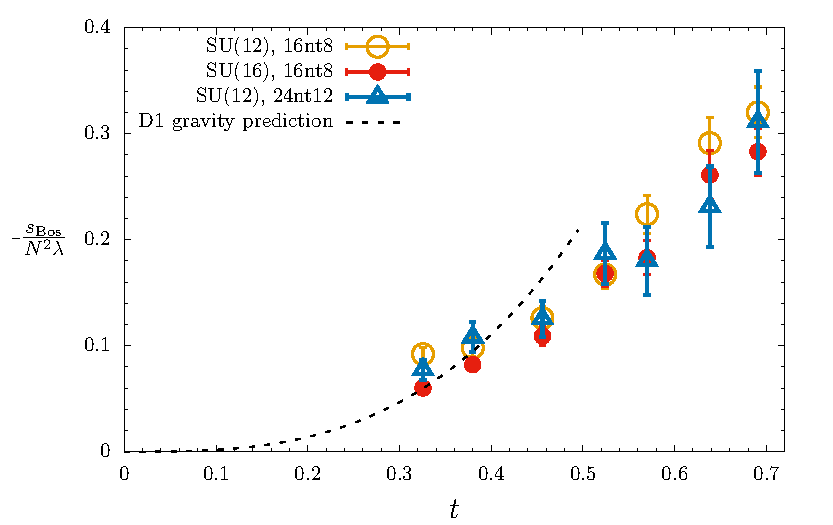
\includegraphics[height=9cm]{Figures/alpha2.pdf}
  \caption{\label{fig:alpha2}Bosonic action density versus dimensionless temperature $t$ for $16\times 8$ and $24\times 12$ lattices (aspect ratio $\al = 2$) with gauge groups SU(12) and SU(16).  All points are results of $\mu^2 \to 0$ extrapolations.  For sufficiently small $t$ our results are in good agreement with the D1-phase gravity prediction, without significant sensitivity to $N$ or the lattice size.}
\end{figure}
\begin{figure}[tbp]
  \centering
  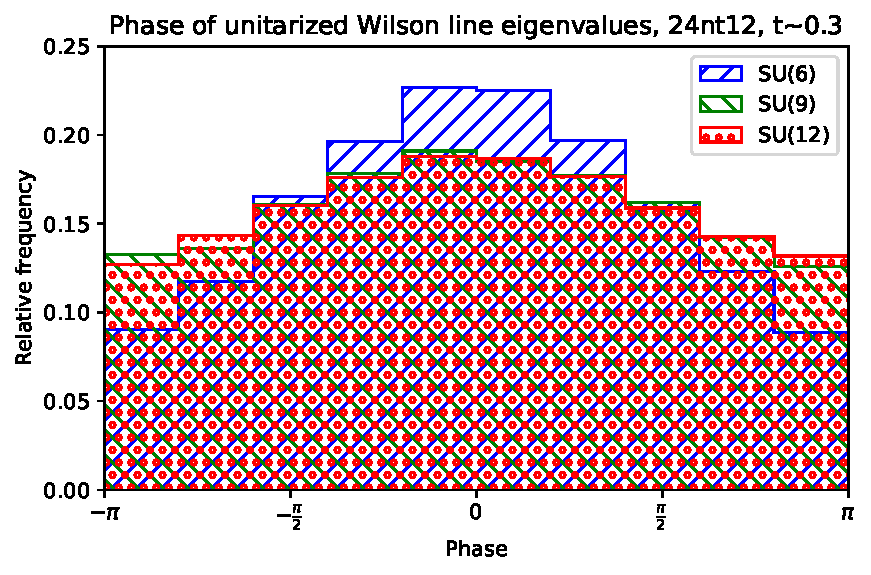
\includegraphics[height=9cm]{Figures/WLeig-al2.pdf}
  \caption{\label{fig:WLeig-al2}Distributions of Wilson line eigenvalue phases, as in figure~\protect{\ref{fig:WLeig-highT}}, for $24\times 12$ lattices at $t \approx 0.33$ with $\mu^2 \approx 0.007$.  The extended distributions, which become more uniform as $N$ increases, correspond to the D1~phase of the gravity dual.}
\end{figure}

In figure~\ref{fig:alpha2} we show the bosonic action density versus $t$ for $\al = 2$ lattice sizes $16\times 8$ and $24\times 12$ with gauge groups SU(12) and SU(16).
From the discussion above, the temperature range shown in the figure lies below the spatial deconfinement transition temperature $t_c \simeq 1.2$.
Hence we expect the system should be spatially confined.
In the low-temperature limit $t \to 0$, we expect it to be described by the gravity D1~phase given in eq.~\eqref{eq:skewD1phase}.\footnote{Eq.~\eqref{eq:skewD1phase} applies directly since $\al, \ga$ lie in the fundamental domain.}
This is corroborated by our lattice results, which lie close to the D1-gravity prediction at low temperatures, $t \lesssim 0.4$.
In a manner similar to the well-studied case of supersymmetric quantum mechanics, this system becomes unstable for very low temperatures, and hence our calculations do not extend all the way down to $t \lesssim 1 / N$.
The origin of this instability is well understood and is discussed in ref.~\cite{Catterall:2009xn}.
The scalar potential terms~\eqref{eq:single_trace} and \eqref{eq:center} help stabilize our numerical calculations, but still do not allow access to arbitrarily low temperatures.
We then need to extrapolate $\mu^2 \to 0$ to remove the soft-$\cQ$-breaking effects of these terms (with $c_W^2 = \mu^2$), which produces the results shown in figure~\ref{fig:alpha2}.
Simple linear $\mu^2 \to 0$ extrapolations generally have good quality with small $\chidof$; we include a representative example in the appendix (figure~\ref{fig:extrap}).
Figure~\ref{fig:WLeig-al2} shows extended distributions for the Wilson line eigenvalue phases on $24\times 12$ lattices at $t \approx 0.33$ (with $\mu^2 \approx 0.007$), which become more uniform as $N$ increases.
This behavior supports our conclusion that the system is spatially confined in this region of the phase diagram, corresponding to the gravity D1~phase.

\begin{figure}[tbp]
  \centering
  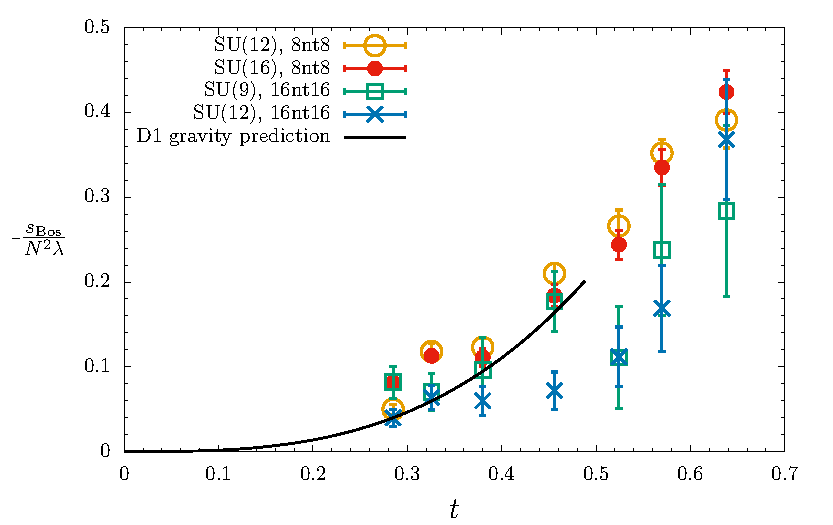
\includegraphics[height=9cm]{Figures/alpha1.pdf}
  \caption{\label{fig:alpha1}Bosonic action density versus dimensionless temperature $t$ for $8\times 8$ and $16\times 16$ lattices (aspect ratio $\al = 1$) with gauge groups SU(9), SU(12) and SU(16).  All points are results of $\mu^2 \to 0$ extrapolations.  Figure~\protect\ref{fig:crit} suggests a transition to the confined phase around $t_c \simeq 0.5$.  For low temperatures $t < 0.4$ our results are in reasonable agreement with the D1-phase gravity prediction (solid curve).  We suspect that the low results for some $16\times 16$ points are artifacts of problematic $\mu^2 \to 0$ extrapolations, suggesting that the uncertainties on these extrapolated results may be underestimated.}
\end{figure}

Next, in figure~\ref{fig:alpha1} we show our corresponding bosonic action density results for $\al = 1$ lattice sizes $8\times 8$ and $16\times 16$.
Although several of the $16\times 16$ points lie significantly lower than the $8\times 8$ points, we suspect that this is not a true finite-size effect but rather an artifact of problematic $\mu^2 \to 0$ extrapolations for the low points.
This suggests that some uncertainties on the extrapolated results may be underestimated.
Figure~\ref{fig:crit} suggests that for $\al = 1$ the deconfinement transition occurs around $t_c \simeq 0.47$.
Thus for $t \lesssim 0.5$ we compare our results to the D1-phase gravity prediction and see a reasonable agreement as $t \to 0$.
Since the deconfinement transition occurs at quite large $t$, we do not expect our results for $t > t_c$ to be well described by the gravity D0-phase behavior, and indeed they are not.
In order to see the gravity D0-phase behavior emerge at low temperature, we need to consider smaller $\al < 1$ so that the transition to confinement occurs at $t_c \ll 1$.

%------------------------
\subsection{D0-phase thermodynamics}
\begin{figure}[tbp]
  \centering
  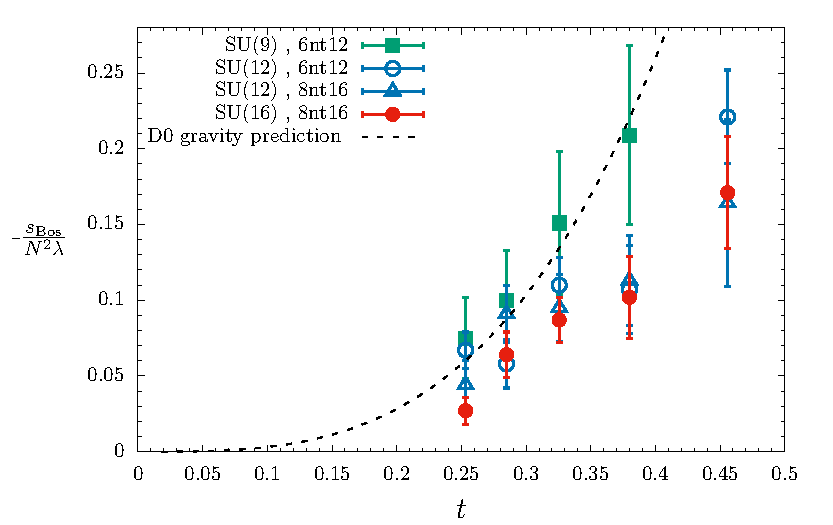
\includegraphics[height=9cm]{Figures/alpha050.pdf}
  \caption{\label{fig:alpha05}Bosonic action density versus dimensionless temperature $t$ for $6\times 12$ and $8\times 16$ lattices (aspect ratio $\al = 1 / 2$) with gauge groups SU(9), SU(12) and SU(16).  All points are results of $\mu^2 \to 0$ extrapolations.  For sufficiently small $t$ our results are in good agreement with the D0-phase gravity prediction.}
\end{figure}
\begin{figure}[tbp]
  \centering
  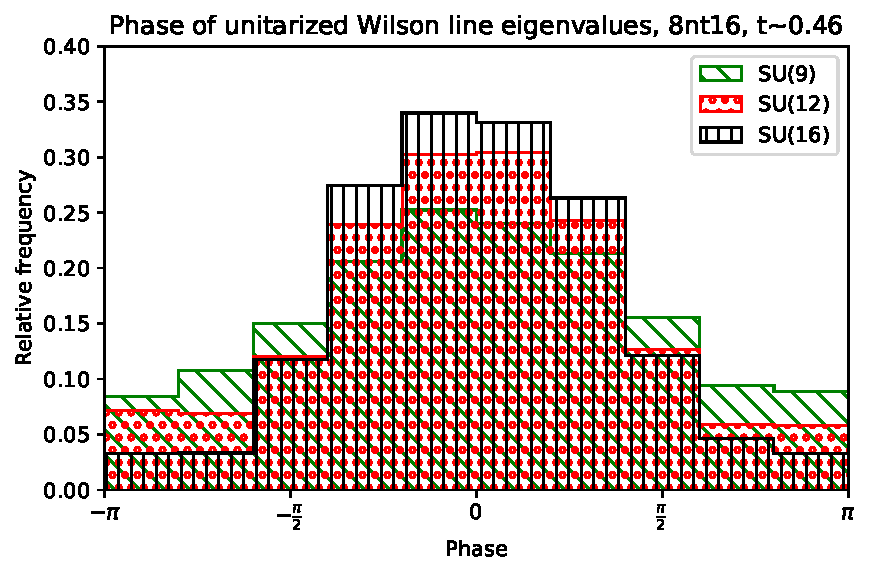
\includegraphics[height=9cm]{Figures/WLeig-al05.pdf}
  \caption{\label{fig:WLeig-al05}Distributions of Wilson line eigenvalue phases, as in figure~\protect{\ref{fig:WLeig-highT}}, for $8\times 16$ lattices at $t \approx 0.46$ with $\mu^2 \approx 0.004$.  The intermediate distributions, which become more compact as $N$ increases, are consistent with expectations from the D0~phase of the gravity dual.}
\end{figure}

The final numerical results we present consider our smallest aspect ratio $\al = 1 / 2$.
Recall from table~\ref{tab:tori} that this lattice geometry is actually equivalent to a rectangular ($\ga' = 0$) torus with $\al' = 1 / \sqrt{3}$, so that $r_{\beta}' = \sqrt{3} r_{\beta} / 2$.
In figure~\ref{fig:alpha05} we plot the bosonic action density for $N = 9$, 12 and 16 from $6\times 12$ and $8\times 16$ lattices.
Again the points shown are results of $\mu^2 \to 0$ extrapolations.
From figure~\ref{fig:crit} we expect the system to be spatially deconfined for the low-temperature range $0.25 \lesssim t \lesssim 0.5$ shown here.
Eventually at very low temperatures, presumably around $t \simeq 0.12$, it should confine, but we are not yet able to probe such a low-temperature regime.
The dashed curve is the low-temperature gravity prediction from the (spatially deconfined) D0~phase, eq.~\eqref{eq:skewD0phase}, which is indeed consistent with the data for $t \lesssim 0.35$.
Figure~\ref{fig:WLeig-al05} shows intermediate distributions for the Wilson line eigenvalue phases on $8\times 16$ lattices at $t \approx 0.46$ (with $\mu^2 \approx 0.004$), which become more compact as $N$ increases.
This behavior supports our conclusion that the system is spatially deconfined in this region of the phase diagram, consistent with the dual gravity approaching the D0~phase in the large-$N$ limit over this temperature range.

%------------------------
\section{Conclusions}
We have studied two-dimensional SYM with maximal supersymmetry compactified on a flat but skewed torus in which an anti-periodic boundary condition is imposed on the fermion fields wrapping one of the cycles.
The theory contains three dimensionless parameters: $r_L$, $r_{\beta} = 1 / t$ and the skewing angle $\cos\theta = \ga$.
From the holographic conjecture, at low `generalized temperature,' $t \ll 1$ this theory should give a description of a dual gravitational system containing various types of black holes arising in Type~IIA and IIB supergravity.
The phase diagram of the gravitational system is expected to contain a region where homogeneous D1 (black-string) solutions dominate and another in which localized D0 (black-hole) solutions dominate.
The critical line separating these two regions in the dual gravitational system is conjectured to be dual to a first-order deconfinement transition with the spatial Wilson loop magnitude $P_L$ serving as an order parameter.

We use lattice gauge theory to explore and test this holographic conjecture using a recently constructed lattice action based on a formalism that maintains exact supersymmetry at non-zero lattice spacing.
The construction singles out a particular skewing angle $\ga = -1 / 2$, which allows us to test holography both for the usual rectangular tori and also---for the first time---for skewed tori as well.

We have mapped out the phase diagram of the SYM system and indeed find a line of transitions separating a spatially confined phase from a deconfined one.
The parametric form of this phase boundary agrees with the results from the gravity dual.
Furthermore, the action density computed in either phase is consistent at low temperatures with the corresponding black hole thermodynamics.
Thus these results can be taken as a new direction to check the predictions of gauge/gravity duality orthogonal to those originating in supersymmetric quantum mechanics. It will be a 
considerable numerical challenge to overcome this. This would certainly need a parallelization over both lattice volume and number of colors. 






\section{\label{app:modular}Modular group and fundamental domain}
Let us recall some facts about the usual modular group $G_{\text{std}}$ and its action on the complex torus parameter $\uptau \in H$, with $H$ the upper half complex plane excluding the real line (so that $\mathrm{Im}(\uptau) > 0$).
The action is given by
\begin{equation}
  \uptau' = \frac{a \uptau + b}{c \uptau + d}
\end{equation}
where $a, b, c, d \in \mathbb{Z}$ and $ad - bc = 1$, which corresponds to an element $\left(\begin{array}{cc} a & b \\ c & d \end{array}\right) \in \text{SL}(2, \mathbb{Z})$.
This group is generated by $S$, $T$ where $S(z) = -1 / z$ and $T(z) = z + 1$.
The fundamental domain for this action on $\uptau$ is
\begin{equation}
  D_{\text{std}} = \left\{\uptau \big| 1 \le |\uptau|, \; - \frac{1}{2} \le \mathrm{Re}(\uptau) \le \frac{1}{2} \right\}.
\end{equation}
In fact we may also take the generators of the group to be $R$ and $T$, where $R(z) = z / (z + 1)$, since $S = T^{-1} R T^{-1}$.
These generators $R$, $T$ are associated to the SL$(2, \mathbb{Z})$ matrices $\left(\begin{array}{cc} 1 & 0 \\ 1 & 1 \end{array}\right)$ and $\left(\begin{array}{cc} 1 & 1 \\ 0 & 1 \end{array}\right)$, respectively.

In this work we are interested in the subset $G$ of the modular group $G_{\text{std}}$ that leaves our fermion boundary conditions invariant, namely the above with $a \in 2 \mathbb{Z}$, $b \in 2 \mathbb{Z} - 1$ and $c \in \mathbb{Z}$.
It is easy to see that $G$ is a subgroup of $G_{\text{std}}$.
The fundamental domain for the action of this new group, $G$, on $H$ is
\begin{equation}
  D = \left\{\uptau\big|1 \le |\uptau \pm 1|, \; -1 \le \mathrm{Re}(\uptau) \le 1\right\}.
\end{equation}
It is generated by the transformations $R(z)$ and $U(z) = T^2(z) = z + 2$, with $R$ as above and $U$ corresponding to the SL$(2, \mathbb{Z})$ matrices $\left(\begin{array}{cc} 1 & 2 \\ 0 & 1 \end{array}\right)$.
We now prove these statements using a simple adaptation of Serre's arguments concerning the domain and generators of the usual modular group~\cite{Serre}.

Following Serre, we firstly consider the subgroup $G'$ of $G$ generated by $R$ and $U$, and later show this is, in fact, the group $G$. \\

\noindent \textit{\underline{Proposition}:} For any $z \in H$ there exists some $g \in G'$ such that $g z \in D$.

\begin{proof}
  Let $z \in H$ and $g$ be an element of the group $G'$ (which is a subgroup of $G$).
  We note that
  \begin{equation}
    \mathrm{Im}(g z) = \frac{\mathrm{Im}(z)}{|c z + d|^2}
  \end{equation}
  and for integers $c, d$ this implies that there exists a $g$ which maximizes $\mathrm{Im}(g z)$.
  Taking such a $g$, then we may choose an integer $n$ so that $z' = U^n g z$ has real part between $\pm 1$.
  In fact $z' \in D$ as we may see by considering $R z'$ and $R^{-1} z'$.
  For any $w \in H$ we have
  \begin{align}
    \mathrm{Im}(R w) & = \frac{\mathrm{Im}(w)}{|w + 1|^2} &
    \mathrm{Im}(R^{-1} w) & = \frac{\mathrm{Im}(w)}{|w - 1|^2}.
  \end{align}
  Thus if $z' \not\in D$, so that either $|z' + 1| < 1$ or $|z' - 1| < 1$, then $g' = R U^n g$ and $g'' = R^{-1} U^n g$ are also elements of $G'$, but either $\mathrm{Im}(g' z) > \mathrm{Im}(g z)$ or $\mathrm{Im}(g'' z) > \mathrm{Im}(g z)$.
  However $\mathrm{Im}(g z)$ was assumed to be maximal, hence we conclude that $z' \in D$.
\end{proof}

\noindent \textit{\underline{Proposition}:} Given two distinct points $z, z' \in D$, then there exists $g \in G$ so that $z' = g z$ only for $z, z' \in \partial D$ (i.e., in the boundary of the fundamental domain).

\begin{proof}
  From the usual arguments about the modular group, we know that for $z \in D_{\text{std}}$ and distinct $z' \in D$ so that $z' = g z$ for $g \in G_{\text{std}}$, then $g = S$, $T$ or $T^{-1}$.
  Hence for distinct $z, z' \in D$ such that $z' = g z$ for $g \in G$ then $g$ is one of $\{S, S^{-1}, T, T^{-1}, T^2, T^{-2}, S T, S T^{-1}, T S, T^{-1} S\}$ (noting that $S^2 = 1$).
  Considering the corresponding SL$(2, \mathbb{Z})$ matrices, we see only the elements $T^2$ and $T^{-2}$ from this list can be elements of $G$, being $U$ and $U^{-1}$, respectively.
  However the only distinct points $z, z' \in D$ related by $g = U$ or $U^{-1}$ are those on the boundaries $\mathrm{Re}(z) = \pm 1$, $\mathrm{Re}(z') = \mp 1$.
\end{proof}

\noindent \textit{\underline{Proposition}:} The subgroup $G'$ is in fact the full group, so $G' = G$.

\begin{proof}
  Consider $z_0 = 2i$ so that $z_0$ is in the interior of $D$.
  Then choose any $g \in G$ and construct $z = g z_0$.
  However, from the first proposition above there exists some $g' \in G'$ such that $z' = g' g z_0 \in D$.
  Thus we have $z_0, z' \in D$, with $z_0 \not\in \partial D$ and $z' = h z_0$ for $h = g' g \in G$.
  However from the above proposition that can only be true for $h = 1$, and hence $g = g'^{-1}$.
  Hence $g \in G'$, and thus $G' = G$.
\end{proof}

A useful corollary of the above construction simply follows that will have physical importance for us in the main text. \\

\noindent \textit{\underline{Corollary}:} Given $\uptau \in D$, then for any $g \in G$ we have $\mathrm{Im}(g \uptau) \le \mathrm{Im}(\uptau)$.

%------------------------
\section{\label{app:scalar}Scalar example: an $A_4^*$ lattice and its dimensional reduction}
Here we consider a scalar field theory in four dimensions discretized on an $A_4^*$ lattice.
We use this to illustrate explicitly the reduction of such a lattice theory to a two-dimensional theory on a $A_2^*$ lattice.
We take a discretization analogous to that we use for $\cN = 4$ SYM, having the lattice action
\begin{equation}
  \label{eq:latscalar}
  S_{\text{lat}} = \frac{1}{\lalat} \sum_{\vn \in \mathbb{Z}^4} \left[\sum_{a = 1}^5 \left[\cD_a \phi(\vn)\right]^2 + \phi(\vn)^4 \right],
\end{equation}
with the lattice derivative taken as
\begin{equation}
  \cD_a \phi(\vn) = \phi\left(\vn + \hatbmu_{(a)}\right) - \phi(\vn).
\end{equation}
The lattice variable $\phi$ lives at lattice sites $\vn \in \mathbb{Z}^4$ and we have included an interaction term and coupling, normalized in analogy with a gauge coupling.
Here the vectors $\hatbmu_{(a)}$ have components $\hat{\mu}_{(\nu)}^{\al} = \delta_{\nu}^{\al}$ for $\al, \nu = 1, \ldots, 4$ and $\hat{\mu}_{(5)}^{\al} = (-1, -1, -1, -1)$.
The kinetic term is differenced symmetrically in these five directions.

Consider continuum coordinates $y^{\mu} = \Delta\, n^{\mu}$ with $\Delta$ the scale setting the lattice size (proportional to the lattice spacing).
Taking the continuum limit $\Delta \to 0$ and assuming a suitably smooth scalar field $\phi$ we may expand
\begin{equation}
  \phi\left(\vn + \hatbmu_{(a)}\right) - \phi(\vn) = \Delta\, \hat{\mu}_{(a)}^{\nu} \left. \pderiv{\phi}{y^{\nu}}\right|_{\vy = \Delta\, \vn}.
\end{equation}
Then, using $\sum_{\vn \in \mathbb{Z}^4} f(\vn) \simeq \frac{1}{\Delta^4} \int d^4 y\, f(y)$ for a (suitably smooth) function $f$ in the $\Delta \to 0$ limit, and defining a continuum field $\Phi = \frac{1}{\Delta} \phi$, the lattice action has the continuum limit $S_{\text{lat}} \to S_{\text{4-cont}}$, where
\begin{align}
  \label{eq:4dact1}
  S_{\text{4-cont}} & = \frac{1}{\lalat} \int d^4 y \left[\sum_{\mu = 1}^4 \left(\pderiv{\Phi}{y^{\mu}}\right)^2 + \left(\sum_{\mu = 1}^4 \pderiv{\Phi}{y^{\mu}}\right)^2 + \Phi^4 \right] \cr
                    & = \frac{1}{\lam_4} \int d^4 y \sqrt{|g|} \Big[g^{\mu\nu} \partial_{\mu} \Phi \partial_{\nu} \Phi + \Phi^4 \Big].
\end{align}
Here the components of the metric are $g_{\mu\nu} = \delta_{\mu\nu} - \frac{1}{5}$, and $|g| = \det{g_{\mu\nu}} = \frac{1}{5}$.
The continuum coupling $\lam_4$ is related to the lattice coupling by $\lam_4 = \lalat / \sqrt{5}$.
We may change to canonical flat-space coordinates $x^{\al} = y^{\mu} e_{(\mu)}^{\al}$, where
\begin{equation}
  e_{(\mu)}^{\al} = \left(\begin{array}{cccc}
     \frac{1}{\sqrt{2}} &  \frac{1}{\sqrt{6}} &  \frac{1}{\sqrt{12}} & \frac{1}{\sqrt{20}} \\
    -\frac{1}{\sqrt{2}} &  \frac{1}{\sqrt{6}} &  \frac{1}{\sqrt{12}} & \frac{1}{\sqrt{20}} \\
     0                  & -\frac{2}{\sqrt{6}} &  \frac{1}{\sqrt{12}} & \frac{1}{\sqrt{20}} \\
     0                  &  0                  & -\frac{3}{\sqrt{12}} & \frac{1}{\sqrt{20}}
  \end{array}\right).
\end{equation}
Then
\begin{equation}
  \label{eq:4dact2}
  S_{\text{4-cont}} = \frac{1}{\lam_4} \int d^4 x \left[\left(\partial_{\al} \Phi\right)^2 + \Phi^4 \right],
\end{equation}
and the lattice sites are located at $x^{\al} = \Delta\, n^{\mu} e_{(\mu)}^{\al}$ for $\vn \in \mathbb{Z}^4$.
Recognizing these $\ve_{(\mu)}$ as basis vectors for the $A_4^*$ lattice, and noting that eq.~\eqref{eq:latscalar} includes a difference also in the direction $\ve_{(5)} = -\sum_{\mu = 1}^4 \ve_{(\mu)}$, we see our original lattice theory is indeed defined on an $A_4^*$ lattice.
While from the explicit coordinate presentation above it isn't obvious, this lattice is maximally symmetric as we should expect from eq.~\eqref{eq:latscalar},
\begin{align}
  \ve_{(a)} \cdot \ve_{(b)} & = \delta_{ab} - \frac{1}{5} &
  a, b & \in 1, \ldots, 5,
\end{align}
and the lattice spacing $a_4$ along all five directions $\ve_{(a)}$ is $a_4 = \Delta \sqrt{4 / 5}$.

Now suppose we are interested in reducing this four-dimensional lattice theory to two dimensions.
We take the lattice variables to be independent of the $\ve_{(3, 4)}$ lattice directions, and restrict the lattice sum $\sum_{\vn \in \mathbb{Z}^4}$ only to a two-dimensional slice of the original four-dimensional lattice, $\vn = (n^1, n^2, 0, 0)$ with $(n^1, n^2) \in \mathbb{Z}^2$.
The lattice action becomes
\begin{equation}
  \label{eq:2dLatticeAct}
  \begin{split}
    S_{\text{lat}}^{\text{(red)}} = \frac{1}{\lalat} \sum_{(n^1, n^2) \in \mathbb{Z}^2} \Bigg[ & \sum_{a = 1}^2 \left(\phi\left(\vn + \hatbmu_{(a)}\right) - \phi(\vn)\right)^2 \\
    & + \left(\phi\left(\vn - \hatbmu_{(1)} - \hatbmu_{(2)}\right) - \phi(\vn)\right)^2 + \phi(\vn)^4 \Bigg]
  \end{split}
\end{equation}
As above, taking continuum coordinates $y^i = \Delta\, n^i$ with $i = 1, 2$, and the continuum limit $\Delta \to 0$, for a suitably smooth function $f$ we have $\sum_{(n^1, n^2) \in \mathbb{Z}^2} f(\vn) \simeq \frac{1}{\Delta^2} \int d^2 y\, f(y)$.
The lattice action has a continuum limit
\begin{align}
  \label{eq:2dact1}
  S_{\text{2-cont}} & = \frac{\Delta^2}{\lalat} \int d^2 y \left[\sum_{i = 1}^2 \left(\pderiv{\Phi}{y^i}\right)^2 + \left(\sum_{i = 1}^2 \pderiv{\Phi}{y^i}\right)^2 + \Phi^4 \right] \cr
                    & = \frac{1}{\lam_2} \int d^2 y \sqrt{|h|} \left[h^{ij} \partial_i \Phi \partial_j \Phi + \Phi^4 \right],
\end{align}
with the metric components $h_{ij} = \delta_{ij} - \frac{1}{3}$ so that $|h| = \frac{1}{3}$ and the two-dimensional continuum coupling $\lam_2 = \lalat / (\Delta^2 \sqrt{3})$.
We may again move to canonical flat-space coordinates $\tilde{x}^m = y^i \tilde{e}_{(i)}^m$ with $m = 1, 2$, where
\begin{equation}
  \tilde{e}_{(i)}^m = \left(\begin{array}{cc}
     \frac{1}{\sqrt{2}} & \frac{1}{\sqrt{6}} \\
    -\frac{1}{\sqrt{2}} & \frac{1}{\sqrt{6}}
  \end{array}\right).
\end{equation}
Then
\begin{equation}
  \label{eq:2dact2}
  S_{\text{2-cont}} = \frac{1}{\lam_2} \int d^2 \tilde{x} \left[\left(\partial_m \Phi\right)^2 + \Phi^4 \right],
\end{equation}
and the two-dimensional lattice sites are now located at $\tilde{x}^m = \Delta\, n^i \tilde{e}_{(i)}^m$ for $\vn \in \mathbb{Z}^2$.\footnote{These coordinate positions are those of the original $A_4^*$ lattice restricted to the 1 and 2~directions, so $\tilde{x}^m = x^m = \Delta\, (n_1, n_2, 0, 0)^{\mu} e_{(\mu)}^m$ for $(n_1, n_2) \in \mathbb{Z}^2$.}
Now defining $\tilde{\ve}_{(3)} = -\tilde{\ve}_{(1)} - \tilde{\ve}_{(2)}$, we see the reduced lattice action, eq.~\eqref{eq:2dact1}, is defined using differences generated by $\left\{\tilde{\ve}_{(1)}, \tilde{\ve}_{(2)}, \tilde{\ve}_{(3)}\right\}$.
We recognize this as a $A_2^*$ lattice action, noting that
\begin{align}
  \tilde{\ve}_{(a)} \cdot \tilde{\ve}_{(b)} & = \delta_{ab} - \frac{1}{3} &
  a, b & \in 1, \ldots, 3,
\end{align}
and the lattice spacing $a_2$ along these three directions $\tilde{\ve}_{(a)}$ is $a_2 = \Delta \sqrt{2 / 3}$.

Finally we note that the two-dimensional continuum action~\eqref{eq:2dact2} is simply the dimensional reduction of the four-dimensional action~\eqref{eq:4dact2}.
More precisely, if we consider the four-dimensional continuum action~\eqref{eq:4dact1} and take the $y^3$ and $y^4$ coordinates to be periodic with period $\Delta$, so that $y^{3, 4} \sim y^{3, 4} + \Delta$, then for $\Delta \to 0$ we may Kaluza--Klein reduce on these directions. 
The zero modes determine the reduced two-dimensional action, which after integrating over the $y^{3, 4}$ directions gives precisely the two-dimensional action~\eqref{eq:2dact1}, with the two- and four-dimensional couplings related by
\begin{equation}
  \label{eq:KKcoupling}
  \lam_2 = \frac{\lam_4}{\Delta^2} \sqrt{\frac{5}{3}}. 
\end{equation}
The factor $\sqrt{5 / 3}$ arises as the Kaluza--Klein reduction is over small periodic directions that are not orthogonal to each other or to the extended $y^i$ directions.

%------------------------
\section{\label{app:num}Numerical details}
We use the standard rational hybrid Monte Carlo (RHMC) algorithm~\cite{Clark:2006fx} implemented in the publicly available parallel software described by ref.~\cite{Schaich:2014pda}.\footnote{{\tt\href{https://github.com/daschaich/susy}{github.com/daschaich/susy}}}
In the course of this work we have improved this software to enable the SU($N$) truncation of the gauge links discussed near the end of section~\ref{sec:lattice_4d}, as well as to add the scalar potential terms in eqs.~\eqref{eq:single_trace} and \eqref{eq:center}.
These additions, along with related improvements to the large-$N$ performance of the code and other advances, will soon be presented in another publication~\cite{parallel_imp}.

\begin{figure}[tbp]
  \centering
  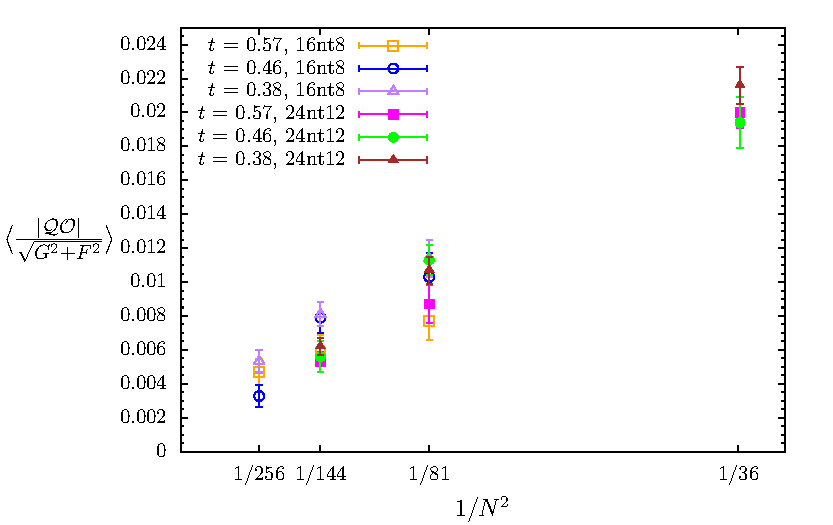
\includegraphics[height=9cm]{Figures/ward.pdf}
  \caption{\label{fig:ward}Violations of a \cQ Ward identity vs.\ $1 / N^2$ for $16\times 8$ and $24\times 12$ lattices (aspect ratio $\al = 2$) with fixed $\mu^2 / \lalat = c_W^2 / \lalat = 0.01$.  The violations are suppressed $\sim 1 / N^2$ and show little dependence on the lattice size or the temperature in the range $0.38 \leq t \leq 0.57$.}
\end{figure}
\begin{figure}[tbp]
  \centering
  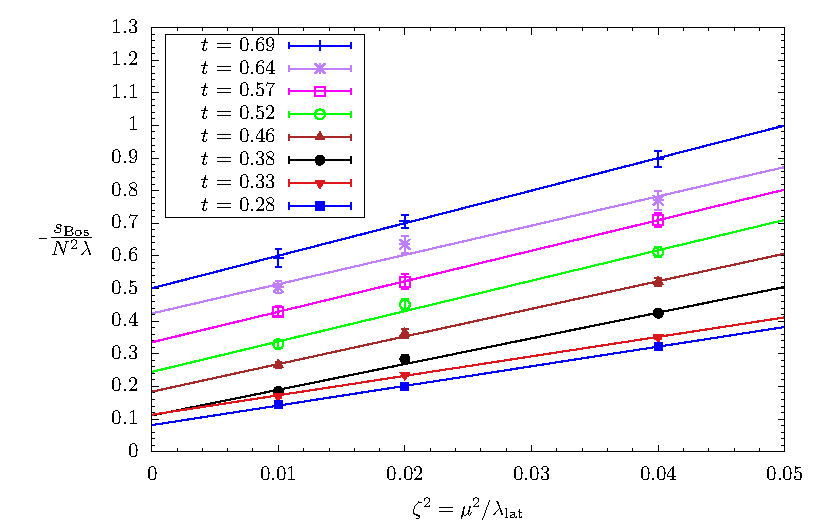
\includegraphics[height=9cm]{Figures/N16_8nt8_extrap.pdf}
  \caption{\label{fig:extrap}A representative sample of linear $\mu^2 \to 0$ extrapolations of bosonic action data for SU(16) $8\times 8$ lattices (aspect ratio $\al = 1$).  The intercepts correspond to the red points in figure~\protect\ref{fig:alpha1}.}
\end{figure}

The results presented in the body of this chapter  involve eight aspect ratios $\al = r_L / r_{\beta} = 1 / 2$, 1, $3 / 2$, 2, $8 / 3$, 4, 6 and 8, investigated for up to five SU($N$) gauge groups with $N = 3$, 6, 9, 12 and 16.
In order to ensure that the soft-$\cQ$-breaking scalar potential terms~\eqref{eq:single_trace} and \eqref{eq:center} introduce only small effects, we require that $\mu^2, c_W^2 \ll \lalat$.
Specifically, as \lalat varies we fix the ratio $\mu^2 / \lalat = 0.01$, 0.02 or 0.04, with either $c_W^2 = 0$ or $c_W^2 = \mu^2$.
In figure~\ref{fig:ward} we show violations of a \cQ Ward identity (discussed in detail by refs.~\cite{Catterall:2014vka, Schaich:2015ppr}), which are small (percent-level at most) and decrease roughly $\propto 1 / N^2$ with fixed $\mu^2 / \lalat = c_W^2 / \lalat = 0.01$.
This establishes that both the scalar potential and the SU($N$) truncation of the gauge links have insignificant numerical effects for sufficiently large $N$.
Finally, in figure~\ref{fig:extrap} we show a representative sample of the linear $\mu^2 \to 0$ extrapolations that produce the results for the bosonic action plotted in figures~\ref{fig:alpha2}, \ref{fig:alpha1} and \ref{fig:alpha05}.
The extrapolations shown here, for SU(16) $8\times 8$ lattices, have acceptable $0.01 \leq \chidof \leq 1.95$ and confidence levels $0.94 \geq \text{CL} \geq 0.16$.
Their intercepts correspond to the red points in figure~\ref{fig:alpha1}.

The RHMC algorithm treats the factor of $e^{-S}$ in the partition function~\eqref{eq:partfunc} as a Boltzmann weight, requiring that the Euclidean action $S$ be real and non-negative.
However, Gaussian integration over the fermion fields of $\cN = (8, 8)$ SYM produces a pfaffian that is potentially complex,
\begin{equation}
  \int \left[d\Psi\right] e^{-\Psi^T \cD \Psi} \propto \pf \cD = |\pf \cD| e^{i\phi},
\end{equation}
where \cD is the fermion operator.
Therefore all our numerical calculations `quench' the phase $e^{i\phi} \to 1$~\cite{Schaich:2014pda}.
In principle, the true expectation values $\vev{\cO}$ can be recovered from phase-quenched (`$_{pq}$') calculations via reweighting,
\begin{equation}
  \vev{\cO} = \frac{\vev{\cO e^{i\phi}}_{pq}}{\vev{e^{i\phi}}_{pq}}
\end{equation}
\begin{align}
  \vev{\cO}_{pq} & = \frac{\int[d\cU] \ \cO e^{-S_B}\ |\pf D|}{\int[d\cU] \ e^{-S_B} \ |\pf D|} &
  \vev{\cO} = \frac{\int[d\cU] \ \cO e^{-S_B}\ \pf D}{\int[d\cU] \ e^{-S_B} \ \pf D}.
\end{align}
Reweighting requires measuring the pfaffian phase $\vev{e^{i\phi}}_{pq}$, and fails if this expectation value is consistent with zero.

\begin{table}[htbp]
  \centering
  \renewcommand\arraystretch{1.2}  
  \addtolength{\tabcolsep}{3 pt}    
  \begin{tabular}{c|c|c|c}
    \hline
    $\al = N_x / N_t$ & $N_x \times N_t$ & $t$  & $1 - \vev{\cos\phi}$     \\
    \hline
    4                 & $16\times 4$     & 4.56 & $37(17)\times 10^{-12}$  \\ 
    \hline
    $3 / 2$           & $12\times 8$     & 0.76 & $55(18)\times 10^{-7}$   \\ 
    \hline
    1                 & $8\times 8$      & 0.38 & $49(17)\times 10^{-7}$   \\ 
                      &                  & 0.76 & $2.93(77)\times 10^{-8}$ \\ 
    \hline
  \end{tabular}
  \caption{\label{tab:pfaffian}Tests of pfaffian phase fluctuations for SU(3) ensembles, considering three aspect ratios \al and a range of temperatures $0.38 \leq t \leq 4.56$.  In all cases $1 - \vev{\cos\phi} \ll 1$ corresponds to very small fluctuations in the phase itself, $\vev{e^{i\phi}}_{pq} \approx 1$ so that phase reweighting has no practical effect.}
\end{table}

Previous lattice studies of $\cN = (2, 2)$ and $\cN = (8, 8)$ SYM theories in two dimensions found $\vev{e^{i\phi}}_{pq} \approx 1$ even at non-zero lattice spacing, with deviations from unity vanishing rapidly upon approach to the continuum limit~\cite{Hanada:2010qg, Catterall:2011aa, Mehta:2011ud, Galvez:2012sv}.
Since we use a different lattice action than those considered previously, for a few SU(3) ensembles we have checked that this remains true in our current work.
Table~\ref{tab:pfaffian} collects the results of these tests, considering $1 - \vev{\cos\phi}$ to ensure that positive and negative fluctuations in $\phi$ cannot cancel out.
In all cases we find $1 - \vev{\cos\phi} \ll 1$, corresponding to $\vev{e^{i\phi}}_{pq}$ close enough to unity that reweighting has no practical effect.









\section{Comments on the hydrodynamics of $D1$-branes}
%It is conjectured that the strong coupling, large $N$ limit of supersymmetric theories possessing sixteen supersymmetries admit a holographic dual
%\cite{Itzhaki:1998dd}. 
In the past couple of years, the program to access and understand the supergravity predictions using numerical simulations of supersymmetric gauge theories have evolved from its nascent stage and good agreement has been observed. Several works \cite{Catterall:2008yz,Hanada:2008ez,Berkowitz:2016jlq} spread over the past decade have checked the thermodynamics
predicted from the supergravity side with the dual gauge theory observables with remarkable success in (0+1)-dimensions. 
The general form of the gauge/gravity duality is valid in lower dimensions as well, however, the four-dimensional case is special because $\mathcal{N}=4$ SYM theory is conformal. Lower dimensions are equally interesting because they can have a rich phase structure and are computationally cheaper to simulate using Monte Carlo methods.
Unlike SYM, the theory of strong interactions (QCD) has no known gravity dual, but QCD at high temperatures (about $T \ge 2.0-3.0~T_{c}$) is nearly a conformal field theory and is thought to be in the same universality class as $\mathcal{N}=4$ SYM. The thermodynamic potentials and transport coefficients have been calculated in 
QCD \cite{Boyd:1996bx, Nakamura:2004sy, Panero:2009tv} and relations to gravity dual via 
AdS/CFT have been explored.  Several important results in strongly coupled QCD have already been obtained using AdS/CFT conjecture, most famously the ratio of shear viscosity ($\eta$) to entropic density, $\eta/s$ up to leading order in $\lambda$. In four dimensions, the only non-trivial 
viscosity coefficient is $\eta$ since the bulk viscosity ($\zeta$) vanishes in $\mathcal{N}=4$ SYM. 
Recently, we explored the two-dimensional supersymmetric gauge theory on a skewed torus and confirmed the phase transition between two different black hole solutions and computed the dual free energy in both phases \cite{Catterall:2017lub, Jha:2017zad}. 
In this proceedings, we \textit{propose} to study the thermodynamics of the gauge theory in more detail by not only calculating the internal/free energy but 
rather the equation of state (EoS) on a square torus (hypercubic trajectories in the moduli space), which in turn will enable us to calculate the speed of the sound,
$\emph{i.e}$ $c_{s}$, the simplest transport coefficient.

\section{Theoretical background}
\subsection{Supergravity predictions}

The IIB supergravity is dual to the `decoupling' limit of $N$ coincident $D1$-branes \cite{Itzhaki:1998dd}. In this limit, 
finite-energy excitations 
are considered simultaneously with the limits, 
$g_{\mathrm{YM}}^{2} = \frac{1}{2\pi} \frac{g_{\mathrm{s}}}{\alpha^{\prime}} = \mathrm{fixed}$ and $\alpha^{\prime}$ $\to$ 0, 
where $g_{\mathrm{s}}$ is the 
string coupling and $\alpha^{\prime}$ is the ~`Regge slope'. In the case of $D1$ branes, one starts out at weak coupling in the UV with 
a perturbative description. In the intermediate regime, there is supergravity (SUGRA) description in terms of $D0/D1$ brane solutions and at 
sufficiently low temperatures, one flows to a free orbifold CFT description. See Figure (\ref{fig:regime}) for a schematic representation of 
different regimes. 
The region in which the strongly coupled Yang Mills theory (denoting $p$ to be number of spatial dimensions) is 
dual to the Type IIA/IIB supergravity is given by, 
\beq\label{ineq:validiity} 
1 \ll \lambda_{\mathrm{eff}} \ll N^{\frac{10-2p}{7-p}} 
\eeq
where,  $\lambda_{\mathrm{eff}} = \lambda_{p+1} \beta^{3-p} = t^{-(3-p)}$, where $\lambda_{p+1}$ is the coupling in 
$(p+1)$-dimensions and $t$ is
the dimensionless temperature. This condition reduces to the familiar $1 \ll \lambda_{4} \ll N$ in four dimensions.
 We will refer to $\lambda_{2}$ and $\lambda$ interchangeably. 

\begin{figure}[htbp]
  \centering
      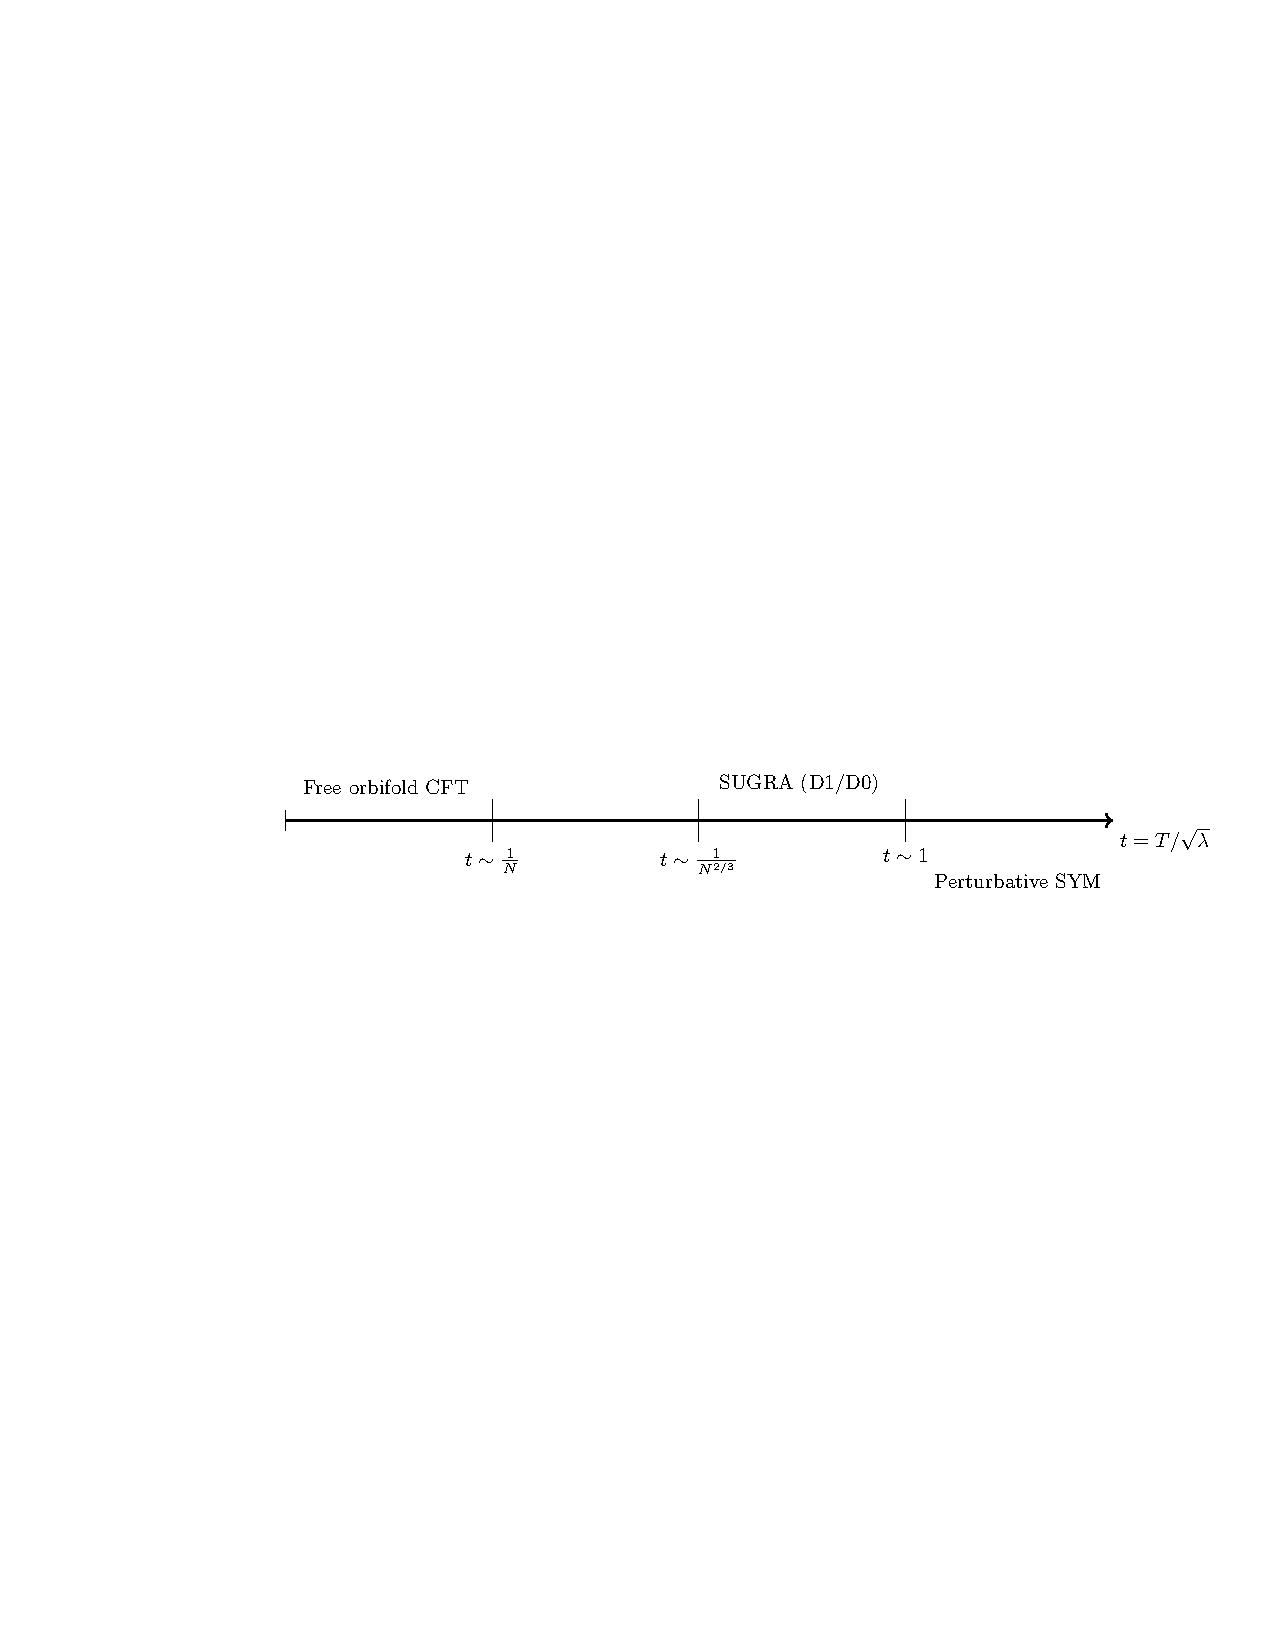
\includegraphics[height=2.51cm]{./Figures/limit.pdf}
  \caption{The different limits of the $\mathcal{N} = (8,8)$ SYM theory. We will focus on the region $1/N^{2/3} < t \ll 1$.}
  \label{fig:regime}
  \end{figure}
Assuming the event horizon of the black hole geometry is at $ U = U_{0}$ (see \cite{Itzhaki:1998dd,Wiseman:2013cda} for details).
Then, we can calculate the temperature associated with the supergravity metric $T$ as,  
\begin{align}\label{eq:temp} 
T = \frac{(7-p) U_{0}^{\frac{5-p}{2}}}{4\pi \sqrt{d_{p} \lambda_{p+1}}}
\end{align}
The corresponding energy can be easily calculated and gives,  
\begin{equation}\label{eq:Energy}
\frac{E}{N^{2}}\Big|_{\mathrm{Dp-brane}} = \frac{(9-p)U_{0}^{7-p} L^{p}}{2^{11-2p} \pi^{\frac{13-3p}{2}} \Gamma\left(\frac{9-p}{2}\right) \lambda_{p+1}^{2}}  
\end{equation}
It can be further shown that, 
\begin{equation}
\frac{E}{S} = \left(\frac{9-p}{14-2p}\right) T 
%E - P = \frac{4P}{5-p}
\end{equation}
and the speed of sound $c_{s}$ is, 

\begin{equation}
c_{s} = \sqrt{\frac{\partial P}{\partial E}} = \sqrt{\frac{5-p}{9-p}} 
\end{equation}
The hydrodynamical coefficients for general Dp-branes, with $p \ge 2$ was calculated in  ~\cite{Mas:2007ng}. 
However, the case $p=1$ is special. It is the only odd $p$, with $p  < 5$ which is not conformal. Also, there is no shear 
viscosity in two dimensions. For D1-branes, it was found in ~\cite{David:2009np} that the speed of sound is 
$c_{s} = \sqrt{\frac{1}{2}}$. The entropy density and bulk viscosity are given by \footnote{Note that there is a typo in 
Equation (5.7) of ~\cite{David:2009np}},  

\begin{equation}
s = \frac{2^4 \pi^{5/2} N^2 T^2}{3^3 \sqrt{\lambda}} 
\zeta = \frac{2^2 \pi^{3/2} N^2 T^2}{3^3 \sqrt{\lambda}} 
\end{equation}
and hence, the ratio $\zeta/s = 1/4\pi$ similar to four dimensions but with $\eta$ replaced by $\zeta$. 
One would ideally expect that $c_{s} = \sqrt{\frac{1}{2}}$ will be obtained for a conformal fluid in (2+1)-dimensions, 
so it is interesting that this result was obtained in a two-dimensional SYM theory in a regime where it is $\emph{not}$ conformal. 
This has been discussed in \cite{Kanitscheider:2009as} where it was argued that the hydrodynamical properties of non-conformal
branes are fully determined in terms of conformal hydrodynamics. The focus of the lattice calculations will be to calculate, $c_{s}$,
over the entire region, where the $D1$-description is valid and provide a numerical outlook on this issue. 

In the well-studied $p=0$ case, there is a single phase since the temporal direction corresponding to the 
black hole horizon is always \emph{deconfined}. For $p=1$, there is an intricate phase structure corresponding to topology changing 
transitions \cite{Gregory:1993vy} also known as the \emph{black hole/black string} transition. Using holography, 
this is conjectured to be dual to the \emph{deconfinement} transition in the gauge theory which for the two-dimensional SYM theory 
is expected to occur around  $r_{x}^2 = c_{\text{gravity}} r_{\tau}$ ($r_{x} = \sqrt{\lambda} L$, $r_{\tau} = \sqrt{\lambda} \beta$), 
and $c_{\text{gravity}} \approx 2.45$ for the square torus \cite{Catterall:2010fx, Dias:2017uyv}. 

Apart from the free/internal energy, EoS and $c_{s}$, there are other interesting observables to measure using 
lattice calculations to compare to
their corresponding gravity predictions. One of these include the Wilson loops proposed in 
~\cite{Rey:1998ik,Maldacena:1998im} for supersymmetric gauge 
theories which also include the contribution from the $(9-p)$ adjoint scalars ($\Phi$). It is defined as follows, 

\begin{equation}
W = \frac{1}{N} \mathrm{Tr} ~ \hat{P} \mathrm{exp} \Bigg[ \oint_C d\tau \Big (A_{\mu}(x) \dot{x}^{\mu} + \hat{\theta}^i|\dot{x}| \Phi_{i}(x)\Big)\Bigg] , 
\end{equation}
where \textbf{$\hat{\theta}$} is the unit vector and C is the contour which is parametrized by 
$x^{\mu}(\tau)$. It is normalized such that large $N$ limit is well-defined. 
We mention the prediction for this observable obtained using supergravity calculations for $ p < 3$, where 
only the $p=0$ case has yet been discussed using numerical simulations \cite{Hanada:2008gy}

\begin{itemize} 
\item $p = 0$ : $ \text{log} ~ \langle W \rangle = 1.89~t^{-3/5}$
\item $p = 1$ : $ \text{log} ~ \langle W \rangle = 1.54~t^{-1/2}$
\item $p = 2$ : $ \text{log} ~ \langle W \rangle = 1.15~t^{-1/3}$  \footnote{Note that this coefficient is little different from one given for potential in \cite{Malacena:Wilson loop}. } 
\end{itemize}  
Generally, $\text{log} ~ \langle W \rangle \sim t^{-(3-p)/5-p}  \sim \lambda_{\mathrm{eff}}^{1/(5-p)}$. Note that
for $\mathcal{N} = 4$ SYM, this gives the $\sqrt{\lambda}$ dependence. 

\subsection{Finite temperature supersymmetric gauge theory} 

We consider the maximally supersymmetric Yang--Mills theory on two-torus ($S^{1}_{\beta} \times S^{1}_{L}$) with anti-periodic 
boundary conditions for the fermions along the time cycle ($\beta = 1/T$) and denote the trace of the energy-momentum
tensor (also known as `trace anomaly' or `interaction measure') by $ \Delta 
= E - P $, where $E$ and $P$ are defined as, 

\begin{equation}
E = T^2 ~ \frac{\partial \text{ln}~ Z}{\partial T}  \bigg\rvert_{V}
P = T ~ \frac{\partial \text{ln}~ Z}{\partial V}  \bigg\rvert_{T}  \label{eq:3}
\end{equation}
Using the approximation for Eq.~(\ref{eq:3}) for homogeneous systems as, 

\begin{equation}
P \approx \frac{T}{V} ~ \text{ln}~ Z ,  
\label{eq:8}
\end{equation}
we can deduce an expression that relates the pressure to $\Delta$ given by, 
\begin{align}
\frac{\Delta}{T^2} &= \frac{E}{T^2} - \frac{P}{T^2} \nonumber  \\  
&= T \frac{\partial}{\partial T} \Big(\frac{P}{T^2}\Big) \label{eq:10}    
\end{align}
Integrating Eq.(\ref{eq:10}) gives, 
\begin{equation}
\frac{P(T)}{T^2} - \frac{P(T_{0})}{T_{0}^2} = \int_{T_{0}}^{T} dT^{\prime} \frac{1}{T^{\prime ~ 3}} \Delta(T^{\prime})
\label{eq:7}
\end{equation}
In principle, this relation will help us determine the EoS and the speed of sound. The range of temperatures ($t = T/\sqrt{\lambda}$ and we set $\lambda = 1$)
considered for the numerical integration would have to satisfy, $ 1/N < t < \alpha^2 / c_{\text{gravity}} $ with $ t \ll 1$. 


\section{Lattice action for the square lattice}

Supersymmetric theories have flat directions which are
a problem for numerical simulations and we control this by adding a $\mathcal{Q}$ breaking term to the lattice action (which we extrapolate to zero) as, 

\begin{equation}
  \label{eq:single_trace}
  S_{\text{flat}} = \frac{N}{4\lambda_{\mathrm{eff}}} \mu^2 \sum_{\textbf{n},\ a \neq 3} \Tr{\bigg(\cUb_a(\textbf{n}) \cU_a(\textbf{n}) - \Ibb_N\bigg)^2}
\end{equation}

Since we are interested in the dimensionally reduced $\mathcal{N} = 4$ SYM to two dimensions with the same number of supercharges 
(known as $\mathcal{N} = (8,8)$ SYM), we dimensionally reduce along the two spatial directions. To have a meaningful dimensional reduction, we have observed that an extra term has to be added to the action given by, 

\begin{equation}
  \label{eq:center}
  S_{\text{center}} = \frac{N}{4\lambda_{\mathrm{eff}}} \mu^2 \sum_{\textbf{n},\ i = x, y} \text{ReTr}\bigg[\bigg(\varphi_i(\textbf{n}) - \Ibb_N \bigg)^{\dagger}\bigg(\varphi_i(\textbf{n}) - \Ibb_N \bigg)\bigg].
\end{equation}

\begin{figure}
\begin{center} 
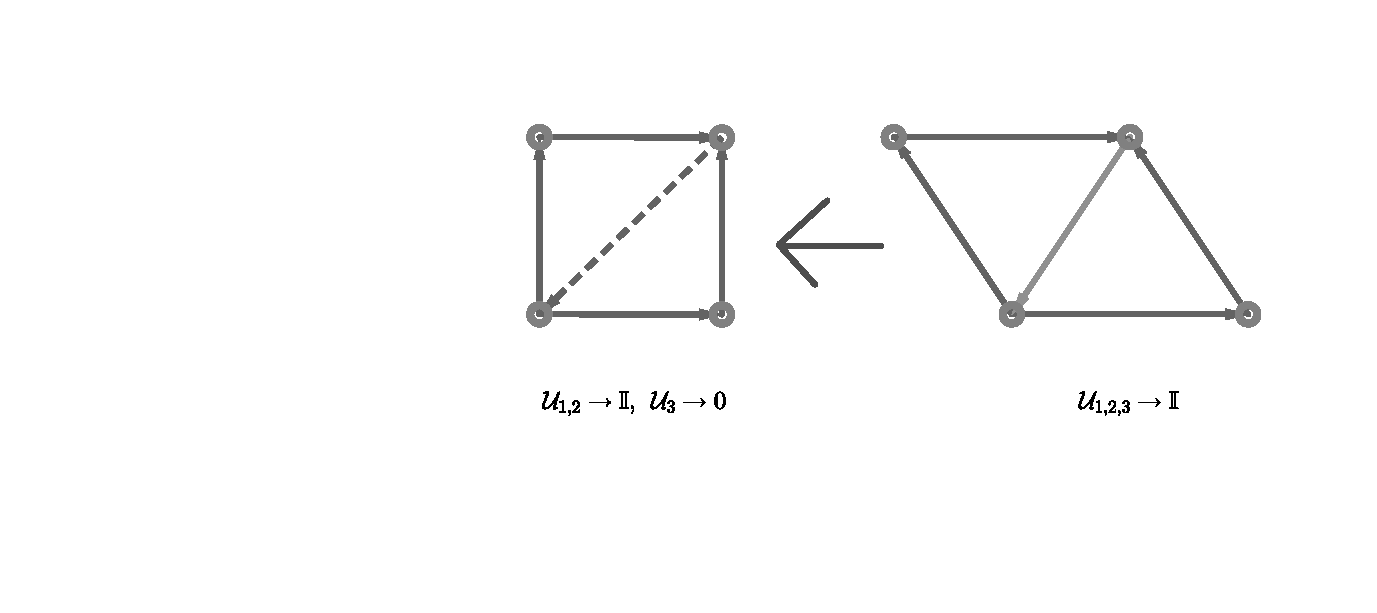
\includegraphics[width=0.72\textwidth]{./Figures/lattice.pdf}
\end{center}
\caption{\label{fig:plot}On the right we have a $A_{2}^{*}$ lattice where the three links are treated equally and expanded symmetrically to 
target the continuum theory. On the left, by modifying the 
third link and requiring that it is expanded around zero, we get square lattice.} 
\end{figure}

The lattice supersymmetric theories based on $\mathcal{Q}$-exact formulation are naturally adapted to non-orthogonal lattices. 
For example,  $\mathcal{N} = 4$ in four dimensions is formulated on $A_{4}^{*}$ lattice which has a bigger point group symmetry than the hypercubic lattice. However, we want to study the two-dimensional 
system on a square lattice. In ~\cite{Unsal:2005yh}, it was argued that one can get different lattice geometries by the choice of the expansion point for the fields in the moduli space (the trajectory one follows to the infinity). We add an additional term, $ S_{A_{2}^{*} \to \text{hyp.}}$ given by, 

\begin{equation}
  \label{eq:hypercubic}
  S_{A_{2}^{*} \to \text{hyp.}} = \frac{N}{4\lambda_{\mathrm{eff}}} \sigma^2 \sum_{\textbf{n}} \Tr{\bigg(\cUb_3(\textbf{n}) \cU_3(\textbf{n})\bigg)^2}
\end{equation}
to the action which consists of the gauge links in the extra direction of the skewed geometry. The resulting lattice 
is square [see Figure (\ref{fig:plot})] when we take $\sigma = O(1)$ fixed for all couplings/temperatures.
The complete lattice action reads,  
\begin{equation}
S = S_{\mathrm{exact}} + S_{\mathrm{closed}} +  S_{\text{flat}} + S_{\text{center}}  + S_{A_{2}^{*} \to \text{hyp.}}
  \label{eq:full_act}
\end{equation}

The numerical simulations should be done sometime in the future using \ref{eq:full_act} on the parallel software \href{https://github.com/daschaich/susy/}{{\texttt{SUSY LATTICE}}}
developed in \cite{Schaich:2014pda}. 




 


\chapter{\label{ch4}Nonperturbative study of dynamical SUSY breaking in $\mathcal{N} = (2, 2)$ Yang-Mills theory}
The investigations of supersymmetric gauge theories on a spacetime lattice are important for understanding the non-perturbative structure of such theories and in particular they can address the question of whether dynamical supersymmetry breaking takes place in such theories. This is a crucial question for efforts to construct supersymmetric theories which go beyond the Standard Model since the low energy world is clearly not supersymmetric while non-renormalization theorems typically ensure that supersymmetry cannot break in perturbation theory \cite{Grisaru:1979wc}.

Unfortunately, there are a plethora of problems to overcome for lattice formulations of supersymmetric theories. Supersymmetry is a spacetime symmetry, which is generically broken by the lattice regularization procedure. Hence, the effective action of the lattice theory typically contains relevant supersymmetry breaking interactions. To achieve a supersymmetric continuum limit it is necessary to  fine tune the lattice couplings to these terms as the lattice spacing is reduced. Since generically there are very many such terms this is in practice impossible.  Some exceptions to this are - $\cN = 1$ super Yang-Mills where only a single coupling, the gluino mass, must be tuned. In addition, it has also been shown that fine-tuning to a supersymmetric
continuum limit is also possible for $\cN = (2,2) $ in two dimensions. Using
Wilson fermions, the only relevant parameter that has to be fine-tuned
is the scalar mass since the bare gluino mass is an irrelevant parameter. The
continuum value for the critical scalar mass is known up to one-loop
order in lattice perturbation theory and that has already been employed in the numerical simulations. See Ref. \cite{Montvay:2001aj, Suzuki:2005dx,August:2018esp} for discussions and references therein. 

The attempt to formulate supersymmetric theories on the lattice has a long history starting in Refs. \cite{Elitzur:1982vh, Banks:1982ut, Sakai:1983dg, Kostelecky:1983qu, Aratyn:1984bc, Scott:1983ha}. Recent approaches to this problem have focused on preserving a subalgebra of the full supersymmetry algebra which can protect the theory from some of these dangerous supersymmetry violating terms - for a review, see Ref. \cite{Catterall:2009it}. For supersymmetric theories with extended supersymmetry various supersymmetric lattice formulations exist. One approach that was pioneered by Cohen, Kaplan, Katz and \"Unsal in Refs. \cite{Cohen:2003xe, Cohen:2003qw, Kaplan:2005ta} is based on orbifolding and deconstruction of a supersymmetric matrix model. A second approach uses the idea of topological twisting to isolate appropriate nilpotent scalar supersymmetries that can be transferred to the lattice. Two independent discretization schemes have been proposed in this approach - that proposed by Sugino in Refs. \cite{Sugino:2003yb, Sugino:2004qd} where the fermions are associated with sites and  a geometrical approach in which fermions are generically associated with links \cite{Catterall:2003wd}\footnote{Yet another construction was formulated by D'Adda, Kanamori, Kawamoto and Nagata, \cite{DAdda:2005rcd} but was later shown to be equivalent to the orbifolding constructions when restricted to a sector containing a scalar supercharge \cite{Damgaard:2007eh}.}. In four spacetime dimensions, the geometrical approach has been used to construct  a supersymmetric lattice action for $\cN = 4$ SYM  \cite{Catterall:2005fd, Catterall:2014vka} and has been shown to be identical to the orbifolding constructions in Ref. \cite{Unsal:2006qp,Catterall:2007kn}. For an elaborate discussion on the relation between all these constructions, see Ref. \cite{Takimi:2007nn}. 

In this chapter, we will study $\cN = (2, 2)$ super Yang-Mills (SYM) theory using the geometrical discretization scheme. It is the simplest two-dimensional supersymmetric theory that can be studied on the lattice. This theory is a particularly interesting theory in the continuum because of its exotic phases as discussed by Witten in Ref. \cite{Witten:1993yc}. This theory is conjectured to flow in the infrared (IR) to a conformal field theory. For recent developments, see Ref. \cite{Park:2016dpb}. The goal  of this chapter is to calculate the vacuum energy density accurately for this theory and hence determine whether supersymmetry breaking occurs. It is well known \cite{Witten:1981nf} that the vacuum energy can be thought of as an order parameter for  SUSY breaking. The spontaneous breaking of supersymmetry in this two-dimensional theory has been considered theoretically in Ref. \cite{Hori:2006dk} and numerically in Refs. \cite{Kanamori:2009dk, Kanamori:2007yx}. In \cite{Hori:2006dk} it was conjectured that in fact supersymmetry may break in this theory. Related work for $\cN = (2, 2)$ super QCD on the lattice was described in \cite{Catterall:2015tta}. In the context of orbifold lattice theories, it was shown in Ref. \cite{Matsuura:2007ec} that the vacuum energy of these theories does not receive any quantum corrections in perturbation theory leaving only non-perturbative mechanisms to drive supersymmetry breaking.

In this four supercharge theory, unlike the sixteen supercharge case in two dimensions, the thermal instabilities at low temperatures are less severe and we can access relatively small temperatures without truncating the $U(1)$ degree of freedom as done in our recent work \cite{Catterall:2017lub, Jha:2017zad}. However, we have to use a small mass term to control the classical flat directions associated with the scalars. This small mass term was also implemented while exploring the phase structure at large $N$ using Sugino's lattice construction in Ref. \cite{Hanada:2009hq}. 

The plan of this chapter will be as follows. In Sec. \ref{sec:theory} we review the lattice construction for $\cN = (2, 2)$ SYM on a two-dimensional square lattice. Then in Sec. \ref{sec:computation} we mention results on the phase of the pfaffian, discuss our procedure of extracting the ground state energy and comment on the $\cO(a)$ improved action we use for the analysis. We end the chapter with conclusions and brief discussion in Sec. \ref{sec:conclude}.

%%%%%%%%%%%%%%%%%%%%%%%%%%%%%%%%%%%%%%%%%%%%%%%%%%%%%%%%%%%
\section{Two-dimensional $\cN = (2, 2)$ Lattice SYM}
\label{sec:theory}
%%%%%%%%%%%%%%%%%%%%%%%%%%%%%%%%%%%%%%%%%%%%%%%%%%%%%%%%%%%

The two-dimensional $\cN = (2, 2) $ SYM theory is the simplest supersymmetric gauge theory which admits topological twisting \cite{Witten:1988ze} and thus satisfies the requirements for a supersymmetric lattice construction following the prescription given in Refs. \cite{Catterall:2004np, Catterall:2006jw}, where the first numerical simulations of this construction were performed. The theory has global symmetry group $G = SO(2)_E \times SO(2)_{R_1} \times U(1)_{R_2}$, where $SO(2)_E$ is the two-dimensional Euclidean Lorentz rotation symmetry, $SO(2)_{R_1}$ is the symmetry due to reduced directions and $U(1)_{R_2}$ is the R-symmetry of the parent four-dimensional $\cN =1$ SYM theory. This theory can be twisted in two inequivalent ways (the A-model and B-model twists) depending on how we embed $SO(2)_E$ group into $SO(2)_{R_1} \times SO(2)_{R_2}$ the internal symmetry group. 

We are interested in the B-model twist, which gives rise to a strictly nilpotent twisted supersymmetry charge. After twisting, the fields and supersymmetries are expressed as representations of the the twisted Euclidean Lorentz group
\beq
SO(2)' = {\rm diag} \Big( SO(2)_E \times SO(2)_{R_1} \Big).
\eeq 
The action of continuum $\cN = (2, 2)$ SYM takes the following $\cQ$-exact form after twisting
\beq
S = \frac{N}{2 \lam} \cQ \int d^2x\,\Psi,
\label{2daction_twisted}
\eeq
where 
%\beq
%\Psi = \Tr \Big( \chi_{ab} \cF_{ab} + \eta [ \cDb_a, \cD_b ] - \frac{1}{2}\eta d \Big),
%\eeq
and $\lam = g^2 N$ is the 't~Hooft coupling. We use an anti-hermitian basis for the generators of the gauge group with $\Tr (T_a T_b)  = - \delta_{ab}$.

The four degrees of freedom appearing in the above action are just the twisted fermions $(\eta, \psi_a, \chi_{ab})$ and a complexified gauge field $\cA_a$. The complexified field is constructed from the usual gauge field $A_a$ and the two scalars $B_a$ present in the untwisted theory: $\cA_a = A_a + iB_a$.
The twisted theory is naturally written in terms of the complexified covariant derivatives
\beq
\cD_a = \partial_a + \cA_a, \quad \quad \cDb_a = \partial_a + \cAb_a,
\eeq
and complexified field strengths
\beq
\cF_{ab} = [\cD_a, \cD_b], \quad \quad \cFb_{ab} = [\cDb_a, \cDb_b].
\eeq
The nilpotent supersymmetry transformations associated with the scalar supercharge $\cQ$ are given by
\bea
\cQ\; \cA_a &=& \psi_a, \nn \\
\cQ\; \psi_a &=& 0, \nn \\
\cQ\; \cAb_a &=& 0, \nn \\
\cQ\; \chi_{ab} &=& -\cFb_{ab}, \nn \\
\cQ\; \eta &=& d, \nn \\
\cQ\; d &=& 0.
\eea
Performing the $\cQ$-variation on $\Psi$ and integrating out the auxiliary field $d$ yields
%\bea
%S &=& \frac{N}{2\lam} \int \Tr \Big( - \cFb_{ab} \cF_{ab} + \frac{1}{2} [ \cDb_a, \cD_a ]^2 \nonumber \\ 
%&-&\chi_{ab} \cD_{\left[a\right.} \psi_{\left.b\right]} - \eta \cDb_a\psi_a \Big). 
%\label{2d-twist_action}
%\eea
The prescription for discretization is straightforward. The complexified gauge fields are mapped to complexified Wilson links
\beq
\cA_a(x) \rightarrow \cU_a(\vn),
\eeq
living on the links of a square lattice with integer-valued basis vectors along two directions, 
\beq
\hatbmu_1 = (1, 0), \quad \quad \hatbmu_2 = (0, 1).
\eeq
They transform in the appropriate way under $U(N)$ lattice gauge transformations
\beq
\cU_a(\vn) \to G(\vn) \cU_a(\vn) G^\dagger(\vn+\hatbmu_a).
\eeq
Supersymmetry invariance then implies that $\psi_a(\vn)$ live on the same links and transform identically. The scalar fermion $\eta(\vn)$ is associated with a site and transforms the following way under gauge transformations
\beq
\eta(\vn) \to G(\vn) \eta(\vn) G^\dagger(\vn).
\eeq
The field $\chi_{ab}(\vn)$, as a 2-form, should be associated with a plaquette. In practice, we introduce diagonal links running through the center of the plaquette and choose $\chi_{ab}(\vn)$ to lie with opposite orientation along those diagonal links. This orientation ensures gauge invariance. Fig. (\ref{fig:lattice-unit-cell}) shows the unit cell of the lattice theory with field orientation assignments. 

%%%%%%%%%%%%%%%%%%%%%%%%%%%%%%%%%%%%%
\begin{figure}[htb]
\begin{center}
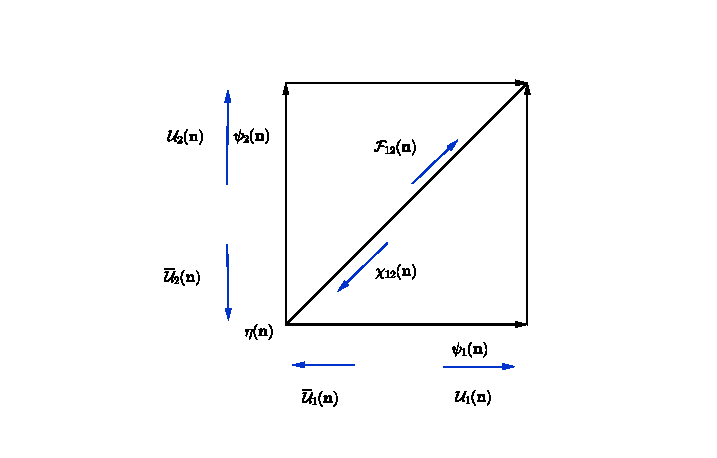
\includegraphics[width=0.95\textwidth]{Figures/lat.pdf}
\end{center}
\caption{\label{fig:lattice-unit-cell}The unit cell and field orientations of the two-dimensional $\cN = (2, 2)$ lattice SYM theory.}
\end{figure}
%%%%%%%%%%%%%%%%%%%%%%%%%%%%%%%%%%%%%

The continuum covariant derivatives are replaced by covariant difference operators and they act on the twisted fields the following way 
\bea
\cDb^{(-)}_a f_a(\vn) &=& f_a(\vn) \cUb_a(\vn) - \cUb_a(\vn - \hatbmu_a) f_a(\vn - \hatbmu_a), \nonumber  \\ 
\cD^{(+)}_a f_b(\vn) &=& \cU_a(\vn) f_b(\vn + \hatbmu_a) - f_b(\vn) \cU_a(\vn + \hatbmu_b). \nonumber 
\eea
The lattice field strength is given by $\cF_{ab}(\vn) = \cD^{(+)}_a \cU_b(\vn)$, and is anti-symmetric. It transforms like a lattice 2-form and yields a gauge invariant loop on the lattice when contracted with $\chi_{ab}(\vn)$. Similarly, the term involving the covariant backward difference operator, $\cDb^{(-)}_a \cU_a(\vn)$, transforms as a 0-form or site field and hence can be contracted with the site field $\eta(\vn)$ to yield a gauge invariant expression.

The lattice action is $\cQ$-exact
\bea
S &=& \frac{N}{2 \lam} \sum_{\vn} \Tr \cQ \Big( \chi_{ab}(\vn) \cD_a^{(+)} \cU_b(\vn) \nonumber \\  
&+& \eta(\vn) \cDb_a^{(-)}\cU_a(\vn) - \hf \eta(\vn) d(\vn) \Big).
\eea
Applying the $\cQ$ transformation on the lattice fields and integrating out the auxiliary field $d$, we obtain the gauge invariant and $\cQ$ supersymmetric lattice action
\bea
\label{eq:2d-latticeaction}
S &=& S_B + S_F,
\eea
where the bosonic action is

%\begin{equation}
%S_{B} = \frac{N}{2 \lambda} \sum_{\vn} \Tr \Big( \cF_{ab}^\dagger(\vn) \cF_{ab}(\vn) + \hf \Big(\cDb_a^{(-)} \cU_a(\vn)\Big)^2\Big), \nonumber 
%\end{equation}

and the fermionic piece
%\begin{equation}
%S_F = \frac{N}{2 \lam} \sum_{\vn} \Tr \Big( - \chi_{ab}(\vn) \cD^{(+)}_{[a} \psi_{b]}(\vn) - \eta(\vn) \cDb^{(-)}_a \psi_a(\vn) \Big). \nonumber 
%\end{equation}
It was correctly noted in Ref. \cite{Kanamori:2008bk} that for simulation purposes, we need to add a small supersymmetry breaking scalar potential to stabilize the $SU(N)$ flat directions of the theory. We add a single trace deformation term to the action in Eq. (\ref{eq:2d-latticeaction}) as, 
%\beq
%\label{eq:single_trace}
%S_{\rm soft} = \frac{N}{2 \lam} \mu^2 \sum_{\vn,\ a} \Tr \bigg( \cUb_a(\vn) \cU_a(\vn) - \Ibb_N \bigg)^2,
%\eeq
with a tunable parameter $\mu$. Exact supersymmetry at $\mu = 0$ ensures that all $\cQ$-breaking terms vanish as some (positive) power of $\mu$.

%%%%%%%%%%%%%%%%%%%%%%%%%%%%%%%%%%%%%%%%%%%%%%%%%%%%%%%%%%%
\section{Lattice Simulations}
\label{sec:computation}
%%%%%%%%%%%%%%%%%%%%%%%%%%%%%%%%%%%%%%%%%%%%%%%%%%%%%%%%%%%

We simulate the theory on a square lattice with anti-periodic boundary conditions (aPBC) for fermions in the temporal direction. The physical size of the lattice is $\beta \times L$, where $\beta$ is the dimensionful temporal extent and $L$ the dimensionful spatial extent. We denote the lattice spacing as $a$ while $N_t$ is the number of lattice sites along the temporal direction and $N_x$ number of sites along the spatial direction. Thus the dimensionful quantities are $\beta = a N_t$ and $L = a N_x$. In our case the lattice is symmetric: $N_t = N_x$. 

In two dimensions, the 't~Hooft coupling $\lambda$ is dimensionful and we can construct the dimensionless temporal circle size, 
\beq
r_\tau = \sqrt{\lambda} \beta.
\eeq
The quantity $r_\tau$ also serves as the effective coupling. Its inverse is the dimensionless temperature $t$. Since we have only considered symmetric lattices, the spatial circle size is the same as the temporal circle size, $r_x = r_\tau$. As discussed above we use a small mass parameter $\mu = \zeta \frac{r_\tau}{N_t} = \zeta \sqrt{\lambda} a$ to regulate potential divergences associated with the flat directions. As for case of sixteen supercharge theory in two dimensions \cite{Catterall:2017lub, Jha:2017zad}, we extrapolate all our results to $\mu = 0$.

To examine the question of supersymmetry breaking we consider the system at non-zero temperature and subsequently take the temperature to zero {\it after} taking the limits $\zeta \to 0$ and $a \to 0$. A non-zero value of the vacuum energy would indicate supersymmetry breaking. Notice that if supersymmetry is intact in a finite volume, it is unbroken even in infinite volume \cite{Witten:1982df}.

We compute the ground state energy density in two-dimensional $\cN = (2, 2)$ SYM using the publicly available code presented in Ref. \cite{Schaich:2014pda}. In the four-supercharge case, the expression for the \emph{effective} bosonic action, which is related to the dimensionless energy density we measure, was first given in Ref. \cite{Catterall:2008dv}. 

We can have two different definitions for the ground state energy based on whether we take the massless (scalar mass) limit followed by the continuum limit or vice versa. In both cases, the zero temperature limit is taken at the end. Thus, we have 
\beq
\label{eq:energy1} 
\frac{\vac^{\prime}}{N^2 \lambda} = \lim_{\beta\to\infty} ~~\lim_{\mathrm{a} \to 0} ~~\lim_{\mu \to 0} \Bigg \langle \mathrm{VAC} \Bigg | \left( \frac{-2\SB}{N^2 \lam} \right) \Bigg | \mathrm{VAC}  \Bigg \rangle,
\eeq
and 
\beq
\label{eq:energy2} 
\frac{\vac}{N^2 \lambda} = \lim_{\beta\to\infty} ~~ \lim_{\mu \to 0} ~~\lim_{\mathrm{a} \to 0} \Bigg \langle \mathrm{VAC} \Bigg | \left( \frac{-2\SB}{N^2 \lam} \right) \Bigg | \mathrm{VAC}  \Bigg \rangle,
\eeq
where, 
\beq
\SB = \frac{1}{L \beta} \left( S_B - \frac{3}{2} N^2 N_x N_t \right).
\eeq 
%%%%%%%%%%%%%%%%%%%%%%%%%%%%%%%%%%%
\begin{figure}[htb]
\begin{center} 
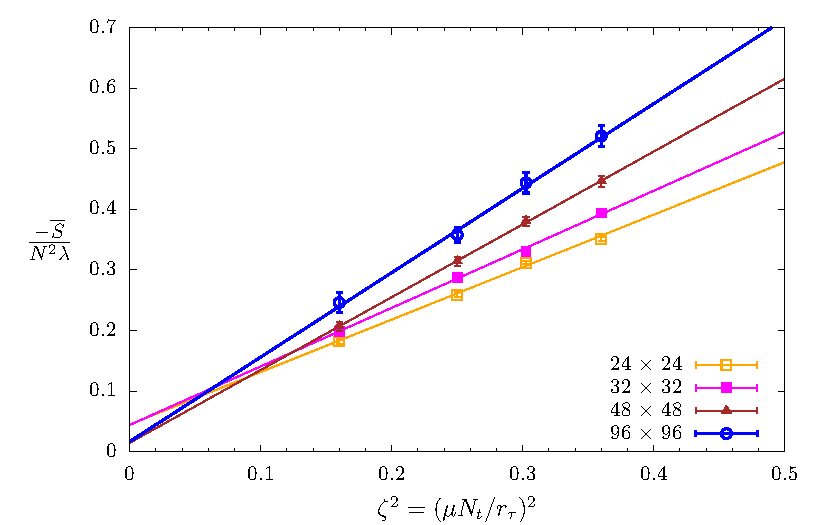
\includegraphics[width=0.95\textwidth]{Figures/mass_U3_rt9.pdf}
\end{center}
\caption{\label{fig:mass_U3}The $\zeta^2 \to 0$ extrapolation of the ground state energy density for $U(3)$, $\RT = 9$.}
\end{figure}
%%%%%%%%%%%%%%%%%%%%%%%%%%%%%%%%%%%
%%%%%%%%%%%%%%%%%%%%%%%%%%%%%%%%%%%
\begin{figure}[htb]
\begin{center} 
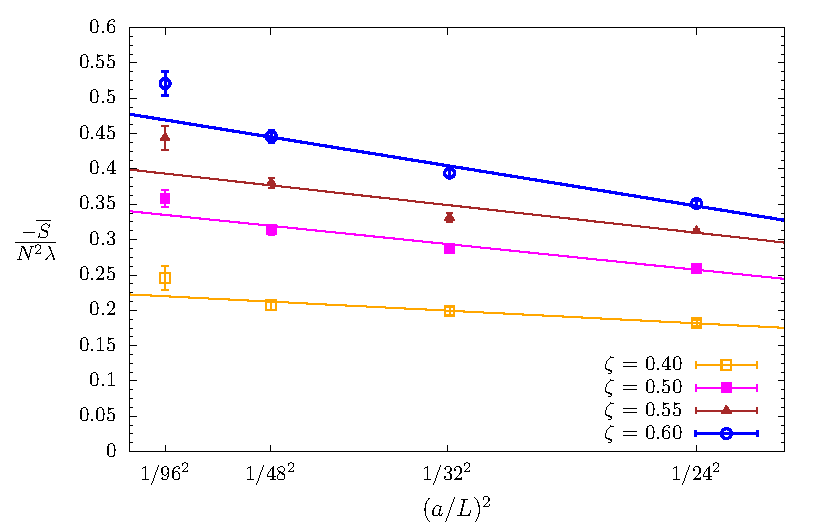
\includegraphics[width=0.95\textwidth]{Figures/cont_U3_rt9.pdf}
\end{center}
\caption{\label{fig:cont_U3}The $(a/L)^2 \to 0$ extrapolation of the ground state energy density for $U(3)$, $\RT=9$.}
\end{figure}
%%%%%%%%%%%%%%%%%%%%%%%%%%%%%%%%%%%
%%%%%%%%%%%%%%%%%%%%%%%%%%%%%%%%%%%%%%%%%%%%%%%%%%%%%%%%%%%

For tables containing the simulation data described in this chapter, please see the appendix of ~\cite{Catterall:2017xox}. 
It is clear from the tables that the order of taking these \emph{different} limits is consistent within errors and we will quote results only for $\frac{\vac}{N^2 \lambda}$.
\begin{figure}[htb]
\begin{center} 
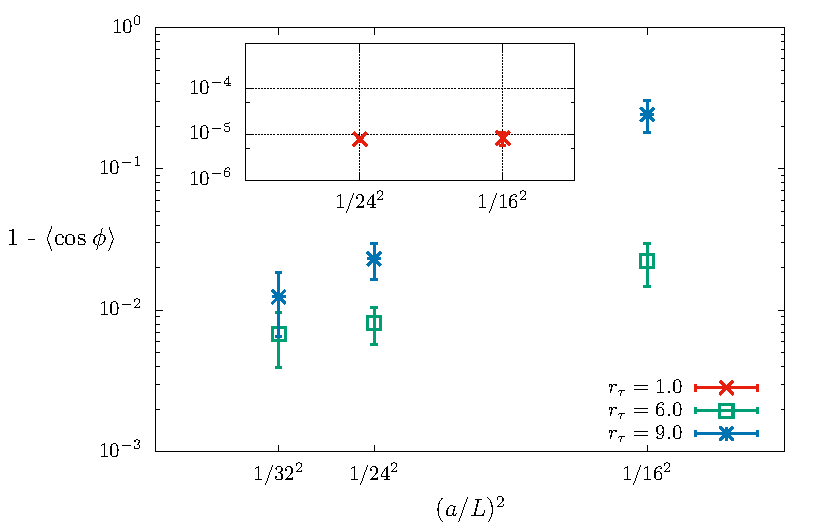
\includegraphics[width=0.95\textwidth]{Figures/2dq4_sign.pdf}
\end{center}
\caption{\label{fig:pfaffian1}Pfaffian phase fluctuations, $1 - \vev{\cos\phi}$, for some U(3) ensembles used in this work. We have measured the phase for three couplings used in this work. We keep the mass parameter, $\zeta = 0.50$ for all couplings. Note that at sufficiently weak couplings, large lattices are not needed to control sign problem.}
\end{figure}
%%%%%%%%%%%%%%%%%%%%%%%%%%%%%%%%%%%
%%%%%%%%%%%%%%%%%%%%%%%%%%%%%%%%%%%
We integrate out the fermions to produce a Pfaffian, which in turn is represented by square root of a determinant. The fermion determinant with a fractional power can be simulated using Rational Hybrid Monte Carlo (RHMC) algorithm \cite{Clark:2004cp}. In the simulations we used the absolute value of the Pfaffian. The phase of the Pfaffian may be incorporated back in the expectation values of observables by re-weighting although as will be seen in the next section the measured Pfaffian phase is always small in our simulations.

%%%%%%%%%%%%%%%%%%%%%%%%%%%%%%%%%%%%%%%%%%%%%%%%%%%%%%%%%%%
\subsection{Phase of the Pfaffian}
\label{sec:pfaf} 
%%%%%%%%%%%%%%%%%%%%%%%%%%%%%%%%%%%%%%%%%%%%%%%%%%%%%%%%%%%

The phase of the Pfaffian was studied in Ref. \cite{Kanamori:2007ye} for two different lattice constructions. Soon after, the phase of Pfaffian for the construction we use here was calculated in Ref. \cite{Catterall:2011aa} and it was observed that it vanishes as one approaches the continuum limit. It was correctly noted in Ref. \cite{Hanada:2010qg} that the absence of the sign is a property of the correct continuum limit. In this chapter, we will study the phase of the Pfaffian at stronger couplings than have been explored before and on much larger lattices using the parallel code developed in Ref. \cite{Schaich:2014pda}. We show that the phase fluctuations become small and vanish as we take the continuum limit. This is true for all couplings we have considered. However, on a fixed lattice volume, the magnitude of the phase fluctuations grows with the coupling. This implies that accessing stronger couplings ($t \le 1/9$) requires the use of larger lattices if we are to avoid a sign problem. We show these results in Fig. \ref{fig:pfaffian1}.
\subsection{Ground State Energy}
\label{sec:ground-state-e}
%%%%%%%%%%%%%%%%%%%%%%%%%%%%%%%%%%%%%%%%%%%%%%%%%%%%%%%%%%%

We now present our simulation results on the ground state energy of the theory. We would like to extrapolate the lattice data for ground state energy density $\frac{\vac}{N^2 \lambda}$ to zero temperature after taking the continuum ($a \to 0$) and massless ($\mu \to 0$) limits. A representative example of the mass extrapolations and continuum extrapolations are shown in Fig. \ref{fig:mass_U3} and Fig. \ref{fig:cont_U3}, respectively.  At the end, we perform three types of extrapolations in temperature - using power law, exponential, and constant fits. 

We show the vacuum energy density vs inverse temperature for $U(2)$ in Fig.~\ref{fig:beta_U2}.
Extrapolating $\RT\to\infty$ using the range $\RT \in [6, 9]$
\beq
\frac{\vac}{N^2 \lambda} = \left\{
  \begin{array}{ll}
    0.06(4), ~ ~ \CHI = 0.40 & : \text{power law fit} \\      
    0.06(2), ~ ~ \CHI = 1.26 & : \text{exponential fit}\\ 
   0.08(2), ~ ~ \CHI = 0.63 & : \text{constant fit}\\  
  \end{array}
\right.
\eeq
In Fig.~\ref{fig:beta_U3} we show the vacuum energy density vs inverse temperature for gauge group $U(3)$.
Extrapolating $\RT\to\infty$ using the range $\RT \in [6, 9]$
\beq
\frac{\vac}{N^2 \lambda} = \left\{
  \begin{array}{ll}
    0.05(2), ~ ~ \CHI = 0.11 & : \text{power law fit} \\  
    0.04(4), ~ ~ \CHI = 0.11 & : \text{exponential fit} \\ 
    0.05(2), ~ ~ \CHI = 0.06 & : \text{constant fit} \\ 
  \end{array}
\right.
\eeq

%%%%%%%%%%%%%%%%%%%%%%%%%%%%%%%%%%%
\begin{figure}
\begin{center} 
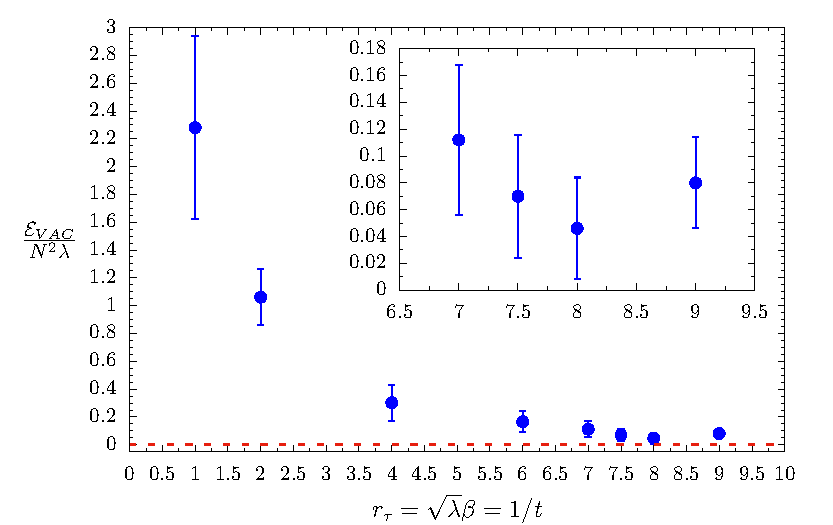
\includegraphics[width=0.95\textwidth]{Figures/beta_U2.pdf}
\end{center}
\caption{\label{fig:beta_U2}The $\beta \to \infty$ extrapolation of the ground state energy for $U(2)$ gauge group. The inset zooms in to show the low-temperature regime.}
\end{figure}
%%%%%%%%%%%%%%%%%%%%%%%%%%%%%%%%%%%
%%%%%%%%%%%%%%%%%%%%%%%%%%%%%%%%%%%%%
\begin{figure}
\begin{center} 
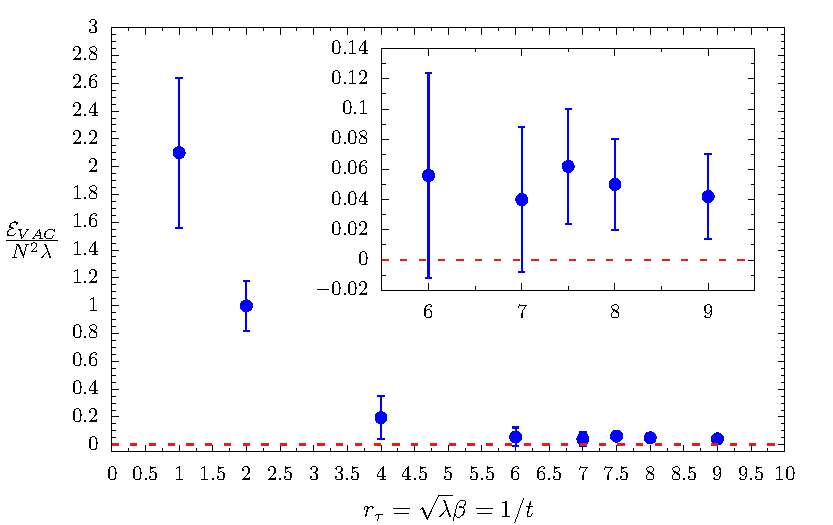
\includegraphics[width=0.95\textwidth]{Figures/beta_U3.pdf}
\end{center}
\caption{\label{fig:beta_U3}The $\beta \to \infty$ extrapolation of the ground state energy for $U(3)$ gauge group. The inset zooms in to show the low-temperature regime.}
\end{figure}
%%%%%%%%%%%%%%%%%%%%%%%%%%%%%%%%%%%%%
We note that the errors in our results do not allow us to make conclusive statements about the exact form of the energy dependence on the temperature. Both power, exponential and constant fitting functions yield
comparable results consistent with vanishing ground state energy.  Our
calculation puts an upper bound on the dimensionless energy density using the constant fit at $\frac{\vac}{N^2 \lambda}=0.08(2)$ for U(2) and $\frac{\vac}{N^2 \lambda}=0.05(2)$ for U(3).

While this work was in progress results were presented on the tree-level $\cO(a)$ improvement of the Sugino's lattice action for two-dimensional $\cN = (2, 2)$ SYM \cite{Hanada:2017gqc}.
We note that our lattice formulation already possesses this improvement which we see in Fig.~\ref{fig:cont_U3} and in
Table \ref{table:order_a}.



%%%%%%%%%%%%%%%%%%%%%
\begin{table}[htbp]
   \vspace{10mm}
      \centering
 \begin{tabular}{cccccc}
\hline \hline
\ \ $\zeta$ \ \ & \ \ $\propto (a/L)^{p} $ \ \ & \ $\propto (a/L)^{p} + c $ \\
\hline
0.40 & 1.86(9) & 1.76(22) & \ \ \\
0.50 & 1.76(6) & 1.60(15) & \ \ \\
0.55 & 1.79(5) & 1.90(11) &  \ \ \\
0.60 & 1.74(4) & 1.70(11) &   \ \ \\
\hline
  %\vspace{4mm}
  
  
  
\end{tabular}
      \centering
 \begin{tabular}{cccccc}

\hline \hline
\ \ $\zeta$ \ \ & \ \ $\propto (a/L)^{p} $ \ \ & \ $\propto (a/L)^{p} + c $ \\
\hline
0.40 & 1.73(10) & 1.58(24) & \ \ \\
0.50 & 1.71(7) & 1.74(17) & \\
0.55 & 1.69(6) & 1.57(14) &  \ \ \\
0.60 & 1.78(5) & 1.98(12) &   \ \ \\
\hline
\end{tabular}

\caption{\label{table:order_a}Numerical results showing that our action is effectively $\cO(a)$ improved. We measure the deviation of the bosonic action/site from its supersymmetric value of $\frac{3}{2}N^2$ and fit it to power law. The first column shows the soft-mass parameter, $\zeta$, we use to regulate the flat directions. The second column is the obtained value of the power, $p$, constraining vanishing intercept, the third is the obtained value of the power, $p$, \emph{without} constraining the intercept. We quote results from one of the couplings used in this work, $\RT$ = 6. On the top, we show the results with $U(3)$ and with $U(2)$ at the bottom. The fits are very good with maximum \CHI = 2.80.}
\end{table}
%%%%%%%%%%%%%%%%%%%%%

%%%%%%%%%%%%%%%%%%%%%%%%%%%%%%%%%%%%%%%%%%%%%%%%%%%%%%%%%%%
\section{Conclusions}
\label{sec:conclude}
%%%%%%%%%%%%%%%%%%%%%%%%%%%%%%%%%%%%%%%%%%%%%%%%%%%%%%%%%%%

In this chapter we have examined the possibility of dynamical supersymmetry breaking in two-dimensional $\cN = (2, 2)$ SYM through lattice simulations. The lattice theory is exact supersymmetric, gauge invariant, local, and doubler free.
We find an upper bound on the vacuum energy density of $\frac{\vac}{N^2 \lambda}=0.08(2)$ and $\frac{\vac}{N^2 \lambda}=0.05(2)$ for U(2) and U(3) respectively. The energy
density is statistically consistent with zero and hence with the absence of dynamical supersymmetry
breaking. It would be interesting to examine the spectrum in future work to confirm the absence of spontaneous supersymmetry
breaking perhaps by searching for signals of a Goldstino as was done in \cite{Catterall:2015tta}. We have also measured the phase of the Pfaffian on all our ensembles and find that while the average
phase grows with coupling it decreases as we take the continuum limit in agreement with theoretical expectations.
In practice, it is numerically small for all our ensembles. 
The question of supersymmetry breaking in this model was addressed before in \cite{Kanamori:2009dk}. Our current work, in addition to using a different lattice action, has employed stronger couplings (and hence
lower temperatures) and much smaller lattice spacings. For example, the lowest temperature used in the earlier work was $t = 1/6$ as compared to $t = 1/9$ in this work while the largest lattice used here is $96\times 96$ as compared
to $30\times 12$ in the earlier study.
 

\chapter{\label{ch5}On the removal of the trace mode in lattice $\mathcal{N} = 4$ super Yang-Mills theory}
In recent years a great deal of effort has been devoted to the construction and numerical studies of
lattice formulations of $\mathcal{N}=4$ super Yang-Mills theory which retain one exact supersymmetry at non-zero
lattice spacing---see the review \cite{Catterall:2009it} and references therein.
These lattice theories 
can be derived using either deconstruction \cite{Cohen:2003xe, Cohen:2003qw, Kaplan:2005ta} or topological field theory methods 
\cite{Catterall:2003wd, Catterall:2005fd, Catterall:2007kn,Unsal:2006qp}. In this approach 
the link fields appearing in the lattice theory take their values in the
algebra of the group, denoted by $\mathfrak{gl}$($N,\mathbb{C})$.\footnote{This 
restriction is not present for Sugino's formulation---see \cite{Sugino:2003yb}.
Other approaches to studying ${\cal N}=4$ super Yang-Mills and the AdS/CFT 
correspondence on a
computer include \cite{Honda:2010nx,Hanada:2008ez,Anagnostopoulos:2007fw,Hanada:2010kt,
Hanada:2013rga,Honda:2011qk,Ishii:2008ib,Ishiki:2008te}.}
This is readily apparent from the (twisted) scalar supersymmetry (SUSY)
transformation
\beq
\cQ \cU_m = \psi_m
\label{impsusy}
\eeq
where $\psi_m$ is a twist fermion that transforms as a link variable.
Since it is a fermion, it has an expansion in terms of generators,
\beq
\psi_m = \sum_{A=0}^{N^2-1} \psi_m^A t^A
\eeq
Here, $t^0$ is proportional to the unit matrix, and must be included
if \ref{impsusy} is to hold, because the link field $\cU_m$ on the
left-hand side certainly has an expansion involving the unit matrix,
if it is to yield the usual $a \to 0$ continuum limit
\beq
\cU_m(x) = 1 + a \cA_m(x) + \cdots
\eeq
(Here, $\cA_m(x)$ is a complexification that contains both the
gauge fields and scalars.)
On the other hand, SUSY should not convert a group valued field into
a Lie algebra valued field, so in fact $\cU_m$ should also have the
expansion
\beq
\cU_m = \sum_{A=0}^{N^2-1} \cU_m^A t^A
\eeq
with the U(1) mode $\cU_m^0$ {\it fully dynamical.}
The conclusion of this argument is that the scalar SUSY $\cQ$
requires the gauge group to be U(N) and not SU(N), with the bosonic
link fields Lie algebra valued.

In the continuum
limit the entire U(1) sector decouples, and becomes an uninteresting free theory---all fields
are in the adjoint representation and hence neutral for U(1).  However on the lattice this sector is coupled
to the SU(N) part through irrelevant operators, so we cannot completely ignore it.  In fact, it is
these irrelevant couplings that can cause various problems. The first of these was first identified in \cite{Catterall:2014vka}
and is manifested in the appearance of a chirally broken phase for 't~Hooft couplings $\lambda_{\text{lat}} > 1$ (see
eqn.~\ref{susyaction} for the definition of the lattice coupling).

Another way to see that the $U(1)$ mode drives instabilities is to examine the behavior of the theory
under the classical
scaling transformation
\begin{eqnarray}
\cU_\mu &\to& c\cU_\mu\\\nonumber
\cUb_\mu &\to& c\cUb_\mu\\\nonumber
\psi_\mu &\to& c^{\frac{3}{2}}\psi_\mu\\\nonumber
\eta &\to& c^{\frac{3}{2}}\eta\\\nonumber
\chi_{\mu\nu} &\to& c^{\frac{3}{2}}\chi_{\mu\nu}
\label{scaling}
\end{eqnarray}
It is trivial to see that the supersymmetric action given
in \cite{Catterall:2014vka} (minus the soft $\cQ$-breaking
mass term) is invariant under this transformation if the Yang-Mills coupling $g^2\to c^4g^2$.
This allows us to write down relations between expectation values of gauge invariant operators. For example,
\beq
\langle {\rm Tr}\prod_{i=1}^P \cU^i \rangle_{g^2}
=c^P \langle {\rm Tr}\prod_{i=1}^P\cU^i \rangle_{c^4g^2}
\eeq
in which we have suppressed spacetime coordinates and indices and where $\cU$ could be replaced by
any other appropriately chosen lattice field with a corresponding change in the multiplicative factor on the RHS.
Since the LHS is independent of $c$ this implies that the expectation value on the RHS must vary as
$c^{-P}$. Note that
this rescaling is not allowed if the link variables $\cU_\mu$ are $SL(N,\mathbb{C})$-valued,
corresponding to gauge group SU(N).  Thus, it is the U(1) sector that creates this
instability.

In \cite{Catterall:2015ira} a new supersymmetric term was added to the lattice action to suppress the $U(1)$ mode
fluctuations. This allows for simulations to be performed out to stronger coupling $\lambda_{\text{lat}} \leq 2$. However,
it does not appear sufficient to explore the regime of extreme strong coupling needed for
studies of S-duality \cite{Giedt:2016wig}. The reason for the ineffectiveness of this term at very strong coupling is
that it constrains only the real part of the determinant of the plaquette operator averaged over all plaquettes
associated with a given lattice site. 

In this chapter, we have attempted to address this problem in a different way by adding to the lattice action
a term which explicitly suppresses the $U(1)$ sector for each link field (we call this the \textit{detlink} term). 
We argue that this term is 1/$N^2$ suppressed and hence the exact scalar SUSY $\cQ$ should be recovered in the large $N$ limit.
Furthermore, we show extensive numerical results that support this conclusion.
The existence of this supersymmetry at large $N$ then guarantees that under
renormalization any $\cQ$-breaking operators that are generated are $1/N^2$ suppressed,
and the scalar SUSY is restored without fine tuning as $N\to\infty$. In addition,
we show that even for modest values of $N$ such as $SU(5)$, $\cQ$ invariance
is a very good approximation.  Early results for this formulation have appeared in \cite{Giedt:2018fxe}. 

An alternate method to achieve the same 
result is by truncating the theory completely to gauge group SU($N$) 
by having links valued in the group $SL(N,\mathbb{C})$ rather than algebra $\mathfrak{gl}$($N,\mathbb{C})$. 
However, the full truncation (bosonic \& fermionic) 
of the theory from U($N$) to SU($N$) does not work. A simple way to see this is as follows: 
Assume a traceless fermion $\psi_a$ which lives on the link in the direction of $e_a$. 
The gauge invariance acts as 
\begin{equation}
\psi_a(x) \to G(x) \psi_a(x) G^\dagger(x + e_a),
\end{equation}
which yields a $\psi_a$ which is not in general traceless. 
Thus we cannot eliminate the $U(1)$ mode of the fermion, even
under the restriction to $SU(N)$ gauge group.\footnote{This is
to be contrasted with \cite{Berkowitz:2016jlq,Rinaldi:2017mjl,Berkowitz:2018qhn} where it was possible to eliminate
the $U(1)$ fermion mode.  This has the benefit of improving
the condition of the fermion matrix.}  Note that this is
a lattice effect, since for a site fermion $\eta$, we would have
\begin{equation}
\mathrm{Tr} G(x) \eta(x) G^\dagger(x) = \eta^A(x) \mathrm{tr} G(x) t^A G^\dagger(x) = \eta^A \mathrm{Tr} t^A = 0
\end{equation}
assuming $\eta(x)$ only involved the generators $t^A$ of $SU(N)$, which are traceless.
The distinction between link fermions and site fermions is only meaningful on the lattice.
This same argument does not apply to the link bosons, since they are valued in the group
and the gauge transformation preserves that feature.

In summary, to maintain lattice gauge invariance, for this {\it hybrid} action 
we only truncate the bosonic sector down to SU($N$). 
This construction also restores $\mathcal{Q}$ supersymmetry 
in the limit $N\to\infty$. In Table \ref{tab:ward-hybrid}, we show the comparison between these two approaches. This method of maintaining
exact lattice supersymmetry by truncating U(1) sector at large $N$ was employed in \cite{Catterall:2017lub,Jha:2017zad} 
to initiate non-perturbative checks of gauge/gravity duality at large $N$ in two dimensions. 
In this chapter, we show detailed numerical results in four dimensions consistent with the claimed $1/N^2$ suppression.

\section{Lattice action}
%
The $\cQ$-exact lattice action takes the form
\begin{align}
  S & = \frac{N}{4\lambda_{\text{lat}}} \sum_x \Tr{\cQ \left(\chi_{ab}\cD_a^{(+)}\cU_b + \eta \cDb_a^{(-)}\cU_a 
- \frac{1}{2}\eta d \right)} + S_{\text{cl}}  \\
  S_{\text{cl}} & = -\frac{N}{16\lambda_{\text{lat}}} \sum_x \Tr{\epsilon_{abcde} \chi_{de}(x + e_a + e_b + e_c) 
\cDb^{(-)}_{c} \chi_{ab}(x + e_c)},
\label{susyaction}
\end{align}
where the lattice difference operators take the form of shifted commutators.
For example,
\begin{equation}
  \cD_a^{(+)} \cU_b(x) = \cU_a(x) \cU_b(x + e_a) - \cU_b(x) \cU_a(x + e_b) \equiv \cF_{ab}(x)
\end{equation}
where $e_a$ are the principle lattice vectors of the $A_4^*$ lattice.
The $\cQ$-closed term is still lattice supersymmetric due to the existence of an exact lattice Bianchi identity,
\begin{equation}
\epsilon_{abcde} \cDb^{(-)}_c \cFb_{ab}(x + e_c) = 0.
\end{equation}
After we integrate out the auxiliary field $d$, we have 
\beq
\label{eq:lat_act}
S  = \frac{N}{4\lambda_{\text{lat}}} \sum_x \text{Tr} \left[ -\cFb_{ab} \cF_{ab} 
+ \frac{1}{2} \left( \cDb_a^{(-)} \cU_a\right )^2 
- \chi_{ab} \cD^{(+)}_{ [a } \psi_{ b] } 
- \eta \cDb^{(-)}_a \psi_a \right] + S_{\text{cl}}.
\eeq
The action also contains a single trace mass term, which helps to lift the classical flat directions by giving a small
mass to the scalar fields:\footnote{It also generates cubic and quartic terms that further stabilize the flat directions.
This mass term has been used for most of our earlier works, and also appears in \cite{Hanada:2010qg}.}
\beq
  \label{eq:single_trace}
  S_{\text{mass}} = \frac{N}{4\lambda_{\text{lat}}} \mu^2 \sum_{x, a} \Tr {\bigg(\cU_a^\dagger \cU_a - \Ibb_N\bigg)^2}.
\eeq
To control the local fluctuations of the $U(1)$ sector we now add a new term to the action:
\beq
\Delta S = \frac{N}{4\lambda_{\text{lat}}} \kappa_\text{link} \sum_{x,a} |\det \cU_a(x) - 1|^2
\label{det}
\eeq
In the limit $\kappa_\text{link}\to\infty$ we can completely remove the $U(1)$ modes --- both gauge and scalar
by restricting the links to SL(N,C). Notice that this term does {\it not} break the $SU(N)$ invariance of the
action since $\det \cU_a(x)$ is invariant under such transformations.
Using a polar decomposition of the link field
\beq
\cU_a(x)=(I+h_a)e^{iB_a}\eeq
the determinant can be written for small $h_a$ and $B_a$ as
\beq
{\rm det}\left(U_a\right)=(1+\frac{1}{\sqrt{N}}h_a^0)e^{i\frac{1}{\sqrt{N}}B_a^0}\eeq
where the $\frac{1}{\sqrt{N}}$ factor arises from the generators which satisfy the normalization ${\rm Tr}(T^aT^b)=-\delta^{ab}$
and the superscript indicates that only the trace mode survives.
To quadratic order in the fluctuations the determinant term becomes
\beq
\Delta S= \frac{1}{4\lambda_{\text{lat}}} \kappa_\text{link} \sum_{x,a} \left(\left(B_a^0\right)^2+\left(h_a^0\right)^2\right)\eeq
The term thus serves to generate masses for the $U(1)$ modes. Additionally, notice it carries no prefactor of $N$ which then
guarantees that it will generate
terms that are $O(1/N^2)$ suppressed relative to the leading terms in a perturbative expansion.

This {\it detlink} term breaks both the $\cQ$-supersymmetry and the $U(1)$  gauge symmetry. Breaking the
$U(1)$ symmetry is likely harmless since the $U(1)$ sector plays no role in the continuum limit.
However breaking the exact supersymmetry is more problematic since it invalidates the arguments given in \cite{Catterall:2014mha}
devoted to the renormalizability of the lattice theory and specifically the number of counterterms needed to
tune to a supersymmetric continuum limit. 

To address this issue, we examine the $N$-dependence of the various terms in the action. It is clear that
the new term being a function of the trace modes only is suppressed by $1/N^2$ as compared to
all other terms in the action which correspond to a sum over all the generators of $U(N)$. 
If we treat this term perturbatively, it will yield a subleading contribution to
any observable in the planar limit. Thus, we expect that 
the exact supersymmetry will be restored in the large $N$ limit. The presence of an
exact supersymmetry at $N=\infty$ then ensures that any SUSY violating operators appearing at 
finite $N$ (and finite $\kappa_\text{link}$) are only multiplicatively renormalized with couplings 
proportional to positive powers of $1/N^2$.
In the next section, we show that these truncated approaches yield stable results 
for a range of values of the 't~Hooft coupling $\lambda_{\text{lat}}$ and measurements of appropriate Ward
identities show the expected $1/N^2$ behavior.

We perform the numerical simulations with the parallel code presented in \cite{Schaich:2014pda}. 
Since then, it has been extended to perform calculations for arbitrary gauge group to access the
large $N$ limit and will be presented in a future publication \cite{parallel_imp}.  We note that
there is an earlier work that develops a method to have $SU(N)$ gauge group in
supersymmetric lattice gauge theory \cite{Kanamori:2012et}.

\section{Ward identities}
%
We test the restoration of $\cQ$ in the large $N$ limit in two ways.\footnote{We note
that while $N=8$ is sufficient for us to see the large $N$ limit in our
four-dimensional lattices, much large $N$ is both necessary and
possible in the case of matrix quantum mechanics \cite{Berkowitz:2016jlq,Rinaldi:2017mjl,Berkowitz:2018qhn}.}  One is via
a measurement of the expectation value of the bosonic action $S_B$,
which is related to an exact lattice Ward identity associated with $\cQ$ in the
original, unmodified theory.
The results on $8^4$ lattice with three different values of $\lambda_{\text{lat}} = 2, 3, 4$
are shown in Fig.~\ref{SBcombo}, with a normalization
such that $S_B = 1$ for exact $\cQ$.  It can be seen that the
restoration is within 1\% in the large $N$ limit, where presumably the
small deviation from $1$ is due to the mass term \ref{eq:single_trace} 
(we take $\mu = 0.1$ in our study) and thermal boundary conditions for the 
fermions along the temporal direction. 

Another check arises through the supersymmetric Ward identity corresponding to
\beq
\Big \langle  \cQ\, {\rm Tr}\,\left(\eta\cU_a\cUb_a\right) \Big \rangle=0\eeq
This yields
\beq
\Big \langle\,{\rm Tr}\, \left(d\cU_a\cUb_a\right)\Big \rangle - \Big \langle\,{\rm Tr}\,\eta \psi_a\cUb_a \Big \rangle=0\eeq
Using the equations of motion to eliminate $d$ we find
\beq
W= \Big \langle\,{\rm Tr}\,\left(\cDb_a \cU_a \cU_b\cUb_b\right)\Big \rangle - \Big \langle\,{\rm Tr}\,\eta \psi_a\cUb_a \Big \rangle=0\eeq
We further normalize $W$ by the fermion bilinear term appearing on the right and take the magnitude, 
\beq
W = \Bigg| \frac{\Big \langle\,{\rm Tr}\,\left(\cDb_a \cU_a \cU_b\cUb_b\right)\Big \rangle - \Big \langle\,{\rm Tr}\,\eta \psi_a\cUb_a \Big \rangle}{\Big \langle\,{\rm Tr}\,\eta \psi_a\cUb_a \Big \rangle} \Bigg|
\label{wardid}
\eeq
to obtain the quantity shown in Fig.~\ref{wdl468}.  It can be seen that the Ward identity, which is zero in the
limit of exact $\cQ$, is approximately $0.6$\% in the large $N$ limit.  Again, we attribute this to the
mass term \ref{eq:single_trace}.

We have also compared these results to the hybrid formulation, where the U(1) sector is
eliminated from the link fields entirely.  In Table \ref{tab:ward-hybrid} it can be seen
that the $\cQ$ violation is more for the \textit{hybrid} than in the \textit{detlink} formulation, but 
with the same 1/$N^2$ dependence. The results for the Ward
identity are shown together in Fig.~\ref{ward_hybrid}.  Thus we see that either approach will
restore $\cQ$ in the large $N$ limit, up to the effects of the regulating mass term.

A final question is the effect of finite volume, given that antiperiodic boundary
conditions are imposed on the fermions.  This also violates the $\cQ$ scalar supersymmetry,
so we expect such effects to fall off with the volume.  It can be seen from Table
\ref{tab:ward-hybrid2} that most of the volume effects are negligible.  Indeed, only
at the weakest coupling for the smallest number of colors is the effect of
any significance.

\begin{figure}
\begin{center}
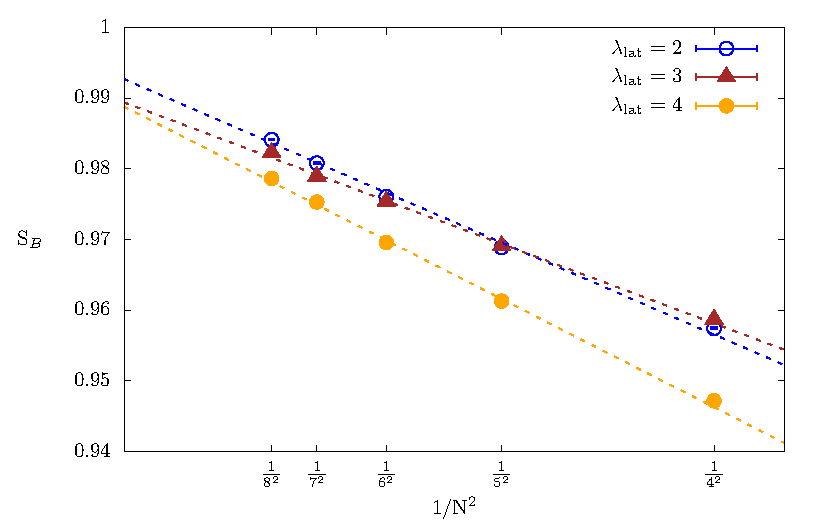
\includegraphics[width=5in]{./Figures/action_detlink_L8.pdf}
\caption{The bosonic action, normalized such that it should be equal to $1$ if
the $\cQ$ symmetry is fully restored (exact).  It can be seen that the $N$ dependence
falls off as $1/N^2$, as expected.  The difference from $1$ in the large $N$
limit is anticipated from the presence of the small
mass term \ref{eq:single_trace} with $\mu=0.1$. Fits to $A + B/N^2$ are also shown in the plot.
For these runs we take $\kappa_\text{link}=5,5,10$ for the three values of $\lambda_{\text{lat}}$ respectively.
\label{SBcombo}}
\end{center}
\end{figure}

\begin{figure}
\begin{center}
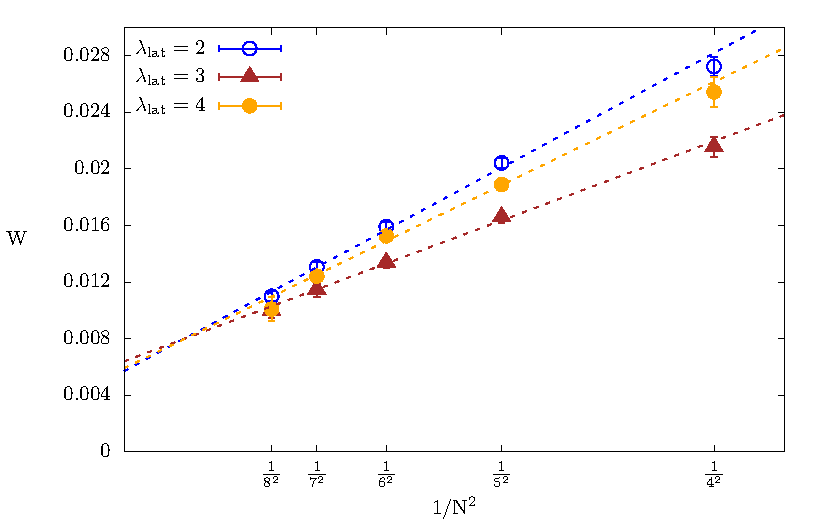
\includegraphics[width=5in]{./Figures/ward_detlink_L8.pdf}
\caption{The Ward identity \ref{wardid} for the $8^4$ lattice with detlink action, 
$\lambda_{\text{lat}}=2,3,4$, $\mu=0.1$ and $\kappa_\text{link}=5,5,10$ respectively. 
Fits to $A + B/N^2$ are also shown. 
\label{wdl468}}
\end{center}
\end{figure}


\begin{figure}
\begin{center}
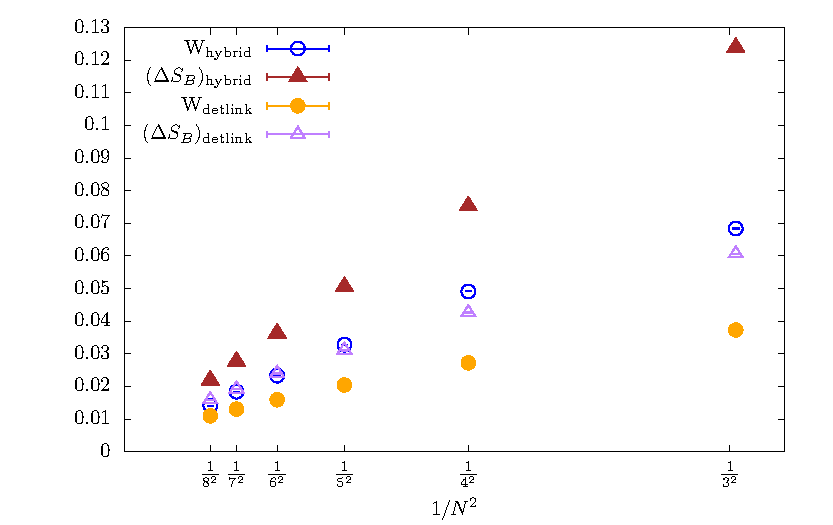
\includegraphics[width=5in]{./Figures/ward_hybrid.pdf}
\caption{\label{ward_hybrid}The comparison between the Ward identity results for the hybrid and detlink cases on $8^4$ lattice for $\lambda_{\text{lat}}=2$. 
In the large $N$ limit, the difference is negligible.}
\end{center}
\end{figure}


\begin{table}
\begin{center}  
\begin{tabular}{cccccccl} 
\hline\hline
$\lambda_{\text{lat.}}$ & $N$ & $\Delta S_{B}$ (detlink) & W (detlink) & $\Delta S_{B}$ (hybrid) & W (hybrid) \\
 \hline 
2.0 & 3 & 0.0606(1)  & 0.0373(8) & 0.1238(4)   & 0.0684(1) \\
& 4 & 0.0426(2)  & 0.0273(7) & 0.0753(2) &  0.0491(0)  \\
& 5 &  0.0311(1) & 0.0204(4)  & 0.0505(1)   & 0.0328(0)  \\
& 6 & 0.0239(1)  & 0.0159(4) &  0.0362(1)  & 0.0233(0)  \\
& 7 & 0.0192(1)  & 0.0131(4) &  0.0276(1)  & 0.0184(0)   \\
& 8 &  0.0159(1) & 0.0110(3) & 0.0218(1)  & 0.0141(0)  \\
\hline  \hline
\end{tabular}
\end{center}
\caption{
\label{tab:ward-hybrid} 
The comparison between the supersymmetry breaking observables using the detlink and the hybrid formulations
on $8^4$ lattice for $\lambda_{\text{lat.}}=2$. $\Delta S_{B}$ denotes the deviation from the supersymmetric value. See Fig.~\ref{ward_hybrid} for details.} 
\end{table}


\begin{table}
\begin{center}
\begin{tabular}{cccccccl} 
\hline\hline
$\lambda_{\text{lat.}}$ & $N$ &  ~~~~~~~~~~~~~~~~~~~~~~~$8^{4}$  &  & ~~~~~~~~~~~~~~~~~~~~~~~$16^{4}$  \\ 
\cline{1-2}
 & & $\Delta S_{B}$ & W  & $\Delta S_{B}$  & W  \\
 \hline 
2.0 & 3 & 0.0606(1)   &  0.0373(8)  & 0.0407(18)   & 0.207(19) \\
& 4 & 0.0426(2) & 0.0273(8) & 0.0425(0) &  0.0281(2)  \\
& 5 &  0.0311(1) &  0.0204(8) & 0.0310(1)   & 0.0202(3)  \\
\hline
3.0 & 4 & 0.0413(2) & 0.0216(7) & 0.0420(2)  & 0.0218(3) \\
& 5 & 0.0309(1)  & 0.0166(4) & 0.0336(1) &  0.0174(4)  \\
\hline
4.0 & 3 & 0.0781(3)  & 0.0336(14) & 0.0788(1)   & 0.0357(3) \\
& 4 & 0.0528(2)  & 0.0254(11) & 0.0521(1) &  0.0230(4)  \\
\hline  \hline
\end{tabular}
\end{center}
\caption{
\label{tab:ward-hybrid2} 
The comparison between supersymmetry breaking observables using the detlink code on $8^4$ and $16^4$ lattices. The volume effects are small
in comparison at fixed $N$.} 
\end{table}

\section{Conclusions}
We have shown that simulations of lattice ${\cal N}=4$ SYM targeting the 
$SU(N)$ rather than the $U(N)$ theory are possible at moderately strong coupling $\lambda_{\text{lat.}} \le 4$. This
is a stronger coupling than has been achieved with the improved action described in \cite{Catterall:2015ira},
where only $\lambda_{\text{lat.}}\le 3$ was possible. 
In the case of gauge group $SU(2)$ simulations have even been performed at $\lambda_{\text{lat.}}=6$. However, unfortunately so far, 
we have not been able to extend this to even stronger couplings. Instead we observe the system appears to undergo a crossover
or phase transition to a regime in which the fermion operator develops very many small eigenvalues. We attribute this
to the presence of residual supersymmetry breaking associated with the determinant term. Work is underway to
develop a supersymmetric link based determinant term which may allow us to bypass these
problems and access yet stronger couplings.  The improvement that we do see is reflective of control
over the instabilities associated with the flat direction exhibited in the scaling \ref{scaling}.
The corresponding U(1) fluctuations are much more dangerous than the SU(N) related
flat directions because they allow the theory to wander into regimes associated with coarser
lattice spacings, where confinement is a generic feature.  In the future, we will
present results where further improvements can be obtained by preserving $\cQ$ exactly
while still controlling this U(1) sector in a rather aggressive way.
 

\newpage 
\chapter{Conclusions}
\epigraph{I think of my lifetime in Physics as divided into three periods. In the first period ...I was in the grip of the idea that 
Everything is Particles...I call my second period Everything is Fields...Now I am in the grip of a new vision that...Everything 
is Information\\ \vspace{3mm} - John A. Wheeler} 

The main theme of the thesis was to explore super-Yang-Mills (SYM) theories in different dimensions on the lattice while preserving exact supersymmetry. Maximally supersymmetric theories play a role in understanding the aspects of holography in more detail. In two dimensions, we studied the phase diagram of the SYM theory and located the deconfinement transition which is related to the transition between two different black hole solutions using holography.  
The horizon topology for four-dimensional black holes is fixed, but when we consider black holes in higher dimensions (such as in Type II supergravity theories), the horizon can have topology change which is holographically dual to the deconfinement transition in the gauge theory at finite temperatures. 
We would also like to study the four-dimensional conformal $\mathcal{N}=4$ SYM 
since most of the holographic predictions are for that theory, but this has been a major obstacle in the past few years even after a series of improvements in the lattice formulation of $\mathcal{N}=4$ SYM. 
The numerical calculations for the four-dimensional theory are very expensive in the large $N$ limit
even with a parallel code over the lattice volume. It is conceivable that constructing a code by parallelizing over $N$ will be possible in the future and will considerably improve our access to supergravity limits using lattice calculations. 
The lower-dimensional SYM theories don't have the sign problem when the fermions have an 
It must also be mentioned that the sign problem in Monte Carlo simulations is another major obstacle in the $\lambda > 5$ studies of SYM in four dimensions with large $N$. It seems that going to stronger coupling in four dimensions would require some new and path-breaking ideas. However, it is certainly possible, as we have shown, to extract interesting Physics from lower-dimensional SYM theories. The twisted lattice action for SYM theories in $d <4$ can still be studied for interesting holographic applications and 
we will continue working on it in coming years. Apart from the thermodynamics of the dual $D2$-branes which is work in progress, we also hope to reproduce the prediction for the static potential in this three dimensional maximally supersymmetric Yang-Mills theory. In order to explore other numerical approaches to gauge theories (than Monte Carlo), 
we have recently studied a two-dimensional non-Abelian gauge theory \cite{Bazavov:2019qih}. 

On the other side, there has been a lot of progress to study the critical systems and their holographic
implications using the tensor network constructions. 
The tensor networks, such as MERA \cite{2008PhRvL.101k0501V} 
have been shown to capture important aspects of holography and offers non-perturbative insights into the geometry of the bulk through the entanglement of the quantum state \cite{Swingle:2009bg, 2015PhRvL.115t0401E, 2011JSP...145..891E, 
2018RvMP...90c5007N, VanRaamsdonk:2009ar, Headrick:2018ctr}.

One of the recent ideas in holography has been the proposal of holographic entanglement entropy (HEE) 
by Ryu-Takayanagi (RT) in 2006 for time-independent geometries. As an example, they considered a time-slice (constant time) 
of $AdS_{3}$ and showed that the entropy matched the one calculated in two-dimensional CFT. 
It was extended to time-dependent geometries by Hubeny, Rangamani, and Takayanagi (HRT) \cite{2007JHEP...07..062H}.
The RT formula says that \begin{equation}
S_{A} = \frac{\text{min.}(Area(\gamma_{A}))}{4G_{N}} \Bigg \vert_{\partial \gamma = \partial A} 
\end{equation} 
The equation above deserves some clarification. The expression tells us to consider only those minimal curves $\gamma$ which satisfies
the homology \footnote{One can think about this in terms of 2-sphere $\mathbb{S}_{2}$. Jordan curve theorem says that any cycle on the sphere can be shrunk to a point. In this sense, all cycles/curves on this manifold satisfy homology condition} condition (\emph{i.e.} those which can be continuously deformed) such that boundary of $\gamma$ is the same as that of $A$. And in case, there is more than one such minimal curve, we choose the one with the smallest area. 
Consider a black hole (whose regions are not simply connected). If we consider that A is the entire-space time, then the boundary of that is an empty set. How does one choose a minimal surface in this situation? $\gamma_{A}$ cannot be empty set since the space-time is not connected. It turns out that the minimal surface is the event horizon. Note that minimal surface is just a curve for $AdS_{3}$.
So, for this case, the HEE formula is just the familiar Bekenstein-Hawking entropy formula. 
If we consider four-dimensional SYM theories on $\mathbb{S}^{3}$ 
at finite temperatures and large $N$, they are expected to undergo Hawking-Page phase transition which is dual to deconfinement transition as discussed above. When the field theory is at zero temperature, the entanglement entropy of the subsystems A $\&$ B is the same. At finite temperatures, the area of minimal curves change and we get a difference in entropy. It is also expected that entanglement entropy can serve as an order parameter. 

It might be interesting to compute the EE on the lattice for supersymmetric theories
in lower dimensions in the future. In all, this is a very exciting and interesting time for different numerical approaches to holography and understanding the features of quantum gravity working at the intersection of high energy theory, quantum information theory, and condensed matter theory.

\newpage



\appendix
\appendixpage
\addappheadtotoc
\section*{\label{app:1RG} \noindent Appendix A.1 Operators and their relevance}
If an operator \cO behaves as $E^{\Delta_{i}}$, then $\Delta_{i}$ is its dimension and $g_{i}$ has units of $E^{D - \Delta_{i}}$, where $D$ is the spacetime dimension. For ex : 
\beq
\frac{1}{2} \int d^D x \partial_{\mu} \phi \partial ^{\mu} \phi 
\eeq
$\phi$ has dimension $E^{D/2 - 1}$. Hence an operator constructed out of A $\phi$'s and B derivatives has 
\beq
\Delta_{i} = A \Bigg (\frac{D}{2} - 1 \Bigg) + B 
\eeq
We can define dimensionless couplings as : 
\beq
\lambda_{i} = \Lambda^{\Delta - D} g_{i} 
\eeq
Note that when $ \Delta_{i} = D$, then $g_{i}$ is dimensionless and we don't need any contruction. 
\bea
\int d^{D} x \cO \sim E^{D - \Delta_{i}} \\ 
\eea 
so that $i^th$ term is of order (in $g_{i}$) 
\beq
\Bigg (\frac{E}{\Lambda} \Bigg)^{\Delta_{i} - D} \lambda_{i} 
\eeq
We see that if $\Delta_{i} > D$, then the term becomes less and less important at low energies. 
If $\Delta_{i} < D$, it becomes more and more important at low energies like $\cN = (8,8)$ SYM in two dimensions. 
The results are shown in Table (\ref{tab:RG1}). 
\begin {table}
 \renewcommand\arraystretch{1.9}   % Increase the height of each row
  \addtolength{\tabcolsep}{2 pt}    % Increase separation between columns
\begin{center}
\begin{tabular}{ |  p{2cm} |  p{2cm} || p{2cm} |c || p{4cm}}
    \hline
    $\Delta_{i}$ & Size in IR & Nature & Property  \\ \hline  \hline
     < D  & Increases  &  Relevant & Super-renormalizable \\ \hline 
     > D  & Decreases &  Irrelevant & Non-renormalizable \\ \hline 
     = D  & Constant & Marginal & Strictly renormalizable \\ \hline
\end{tabular}
\vspace{3mm}
\caption {\label{tab:RG1}Dimension of operators, size in the IR, nature and property of the theory.} 
\end{center}
\end {table}




\section*{\label{app:2spinors} Appendix A.2 Spinors in various dimensions}

We have often come across notations like $\mathcal{N} = (2,2)$ and $\mathcal{N} = (8,8)$ in the main text. This is different from the notation we are used to in four dimensions. In 4d, the Weyl representation is complex, so that the representation of $\overline{Q}$ is fixed to be the conjugate of the Q representation. In 2d, the Weyl representation is real ($\textit{Majorana-Weyl}$) and the $\overline{Q}$ representation is independent of the Q representation. This can be seen for various dimensions from Table (\ref{tab:spinor}). 

\begin {table}[htbp] 
\begin{center}
\begin{tabular}{ |  p{3cm} | l | l |  l | p{3cm} |}
    \hline
    \textbf{Dimensions(d)} & \textbf{Majorana} & \textbf{Weyl} & \textbf{Weyl-Majorana}  & \textbf{Min.Rep} \\ \hline \hline 
     2 & Yes & Self & Yes & 1 \\ \hline 
     3 & Yes & - & - & 2 \\ \hline
     4 & Yes & Complex & - & 4 \\ \hline
     5 & - & - & - & 8 \\ \hline
      6 & - & Self & - & 8 \\ \hline
     7 & - & - & - & 16 \\ \hline
     8 & Yes & Complex & - & 16 \\ \hline
     9 & Yes & - & - & 16 \\ \hline
     10 (\textit{mod 8}, 2) & Yes & Self & Yes & 16 \\ \hline
     11 (\textit{mod 8}, 3) & Yes & - & - & 32 \\ \hline
     12 (\textit{mod 8}, 4) & Yes & Complex & - & 64 \\ \hline
\end{tabular}
\vspace{3mm}
\caption {\label{tab:spinor} Dimensions in which various conditions are allowed for $SO(d-1,1)$ spinors} 
\end{center}
\end {table}


\section*{\label{app:3sugra} Appendix A.3 Type II SUGRA details}
When the consider the black hole solutions at finite temperature, the temperature, $T_{H}$ is given by : 
\begin{equation}
\label{eq:temp_SUGRA}
T \propto \frac{(7-p) U_{0}^{(5-p)/2}}{4 \pi \sqrt{d_{p} \lambda}}
\end{equation}
for a uniform black $p$-brane solution. The $ \alpha^{\prime}$ corrections can be written in terms of $U_{0}$ as, 
\begin{equation}
  \label{eq:alpha_prime}
\alpha^{\prime} R \propto \sqrt{\frac{U_{0}^{(3-p)}}{\lambda}}
\end{equation}
We see from \ref{eq:temp_SUGRA} and \ref{eq:alpha_prime} that $ \alpha^{\prime} R \propto t^{\frac{3-p}{5-p}}$\footnote{The dimensionless temperature $t$, is constructed 
from $T$ by combining with appropriate powers of $\lambda$} and hence, $ (\alpha^{\prime})^3$ correction depends on $t^{\frac{9-3p}{5-p}}$. This power counting has been discussed in \cite{Berkowitz:2016jlq}.


%%%%%%%%%%%%%%%%%%%%%%%%%%%%%%

\section*{\label{app:4energy} Appendix A.4 Free energy results for SYM theories}

Some useful integrals in the study of thermodynamics of weak coupling limit of SYM theories are, 
\begin{equation}
    \int_{0}^{\infty} \frac{x^{d-1}}{e^{x} -1} dx = \Gamma(d)\zeta(d) 
\end{equation}

\begin{equation}
    \frac{7}{8}\int_{0}^{\infty} \frac{x^3}{e^{x} -1} dx = 
    \int_{0}^{\infty} \frac{x^3}{e^{x}+1} dx = \frac{7\pi^4}{120} 
\end{equation}

\begin{equation}
    \frac{3}{4}\int_{0}^{\infty} \frac{x^2}{e^{x} -1} dx = 
    \int_{0}^{\infty} \frac{x^2}{e^{x}+1} dx = \frac{3 \zeta(3)}{2}
\end{equation}

\begin{equation}
    \frac{1}{2}\int_{0}^{\infty} \frac{x}{e^{x} -1} dx = 
    \int_{0}^{\infty} \frac{x}{e^{x}+1} dx = \frac{\pi^2}{12}
\end{equation}
In (3+1)-dimensions, the fermionic degrees of freedom contribute 7/8 of bosonic ones. In sixteen supercharge case, 
we get,  
\begin{equation}
N^2 \left[ 8 + (7/8)8 \right] = 15N^2
\end{equation}
In general, total d.o.f in $d$ dimensions will be, 
\begin{equation}
8 \Big( 2 - \frac{1}{2^{d-1}}\Big) N^2
\end{equation}
Black body radiation gives 
\begin{equation} 
E = \frac{VT^4 \pi^2}{30} ~~~\text{per d.o.f}
\end{equation} 
For $\mathcal{N}=4$ SYM in four dimensions, we have 
\begin{equation} 
E = 15N^2 \frac{VT^4 \pi^2}{30} 
\end{equation} 
and the entropy is,  
\begin{equation} 
S = \frac{2\pi^2}{3} VT^3N^2 
\end{equation} 
The free energy is given by, 
\begin{equation}
F = \frac{-\pi^2}{6} VT^4N^2 
\end{equation} 
%This has also be  by Klebanov and Tsetylin at zero $\lambda$. 
%Also, see Zweibach Page 557
A similar analysis in 3d gives, 
\begin{equation}
E =  \frac{14\zeta(3)}{\pi}VN^2T^3 
\end{equation} 
The entropy is given by,  
\begin{equation}
S = \frac{21\zeta(3)}{\pi}VN^2T^2
\end{equation} 
and free energy F is ($g_{\text{YM}} \to 0$) 
\begin{equation}
F = \frac{-7\zeta(3)}{\pi}VN^2T^3
\end{equation} 
%Matches arxiv 9905030 
The free energy density for ${\cal N}=4$  SYM in the weak coupling regime is :
\begin{equation}
    f = \frac{F}{V} = - \left(4 + 2n_{s} + \frac{7}{2} n_{f}\right) N^{2} \zeta(4) T^{4} \frac{1}{V} 
\end{equation}
Here, V is the unit volume of three sphere $S^{3}$ = $2\pi^2$. 
Two interesting limits to this expression :
\begin{itemize}
\item Only gauge: $n_{s} = 0$, $n_{f} = 0$ gives $f = - \frac{\pi^2}{45} N^{2}T^{4}$, which is the photon gas result! 
\item Full theory: $n_{s} = 6$, $n_{f} = 4$ gives $f = - \frac{\pi^2}{6} N^{2}T^{4}$
\end{itemize}

%%%%%%%%%%%%%%%%%%%%%%%%%%%%%%


\section*{\label{app:5dforms} Appendix A.5 Differential forms}

The lattice construction of super Yang-Mills theories on the lattice makes use of special kind of fermions which are 
integer forms rather than spinors. Here, we will briefly review the important results of differential forms. 
See ~\cite{Zumino:1983rz} ~\cite{MTW} for further details. 
A scalar function is called a \emph{0-form} and is defined as : 
\beq
df \equiv \frac{\partial f}{\partial x^{\mu}} dx^{\mu} 
\eeq 
Suppose we have a vector function $\Phi_{\mu}$, we construct a \emph{1-form} $\Phi$ as $ \Phi = |phi_{\mu} dx^{\mu}$. 
and define, 
\beq
d \Phi \equiv \frac{\partial \Phi_{\mu}}{\partial x^{\nu}} dx^{\nu} \wedge dx^{\mu} 
\eeq 
The $\wedge$ denotes the wedge product defined as : 
\beq
dx^{\nu} \wedge dx^{\mu}  = - dx^{\mu}  \wedge dx^{\nu}
\eeq
We can interpret $d\phi$ as curl of $\Phi$. 
Generally, from an anti-symmetric tensor with p-indices, 
we can construct a \emph{p-form} as, 
\beq
\Phi = \Phi_{\mu_{1}, \mu_2, \cdots \mu_{p}} \Bigg( \frac{1}{p!} dx^{\mu_1} \wedge dx^{\mu_2} \wedge \cdots dx^{\mu_p} \Bigg)  
\eeq
It is obvious that we cannot have p-forms with $p > D$, where D is the number of dimensions. 
\beq
d\Phi = \partial_{\nu} \Phi_{\mu_{1}, \mu_2, \cdots \mu_{p}} \Bigg( \frac{1}{p!} dx^{\nu} \wedge dx^{\mu_1} \wedge dx^{\mu_2} \wedge \cdots dx^{\mu_p} \Bigg)  
\eeq
Let's take a \emph{p-form} $\alpha$ and \emph{q-form} $\beta$, 
then we have 
\beq
\alpha \beta = (-1)^{pq} \beta \alpha 
\eeq 
Then, 
\beq
d(\alpha \beta) = (d\alpha)\beta + (-1)^{p}\alpha d(\beta)
\eeq 
In YM theory, the gauge potential is \emph{1-form} 
\beq
A = A_{\mu} dx^{\mu} 
\eeq 
and, field tensor F is defined schematically as \footnote{$F = \frac{1}{2} (\partial_{\mu} A_{\nu} - \partial_{\nu} A_{\mu} + [A_{\mu}, A_{\nu}]) dx^{\mu} dx^{\nu}$} 
\beq
F = dA + A^{2} 
\eeq 
with, 
\bea
dF & = d(dA + A^{2})  \\ 
     & = d(AA) \\
     & = d(A)A - AdA \\
\eea 
Also, 
\beq
[A, F] = [A, dA] = AdA - dAA 
\eeq
Adding above two, we get (Bianchi identity from forms) 
\beq
DF \equiv dF + [A, F ] = 0 
\eeq
where, $D (\cdot) = d (\cdot) + [A, (\cdot)]$. 


\section*{\label{app:6pfaffian} Appendix A.6 Note on Pfaffian}

Let M be a complex $d \times d$ matrix which is anti-symmetric (also known as skew-symmetric, $M^{T} = -M$), then we have $\text{det}M = 0$, if d = odd. Therefore, we will assume that $d = 2n$. 
For an even-dimensional complex $ 2n \times 2n$ matrix, pfaffian is defined as, 
\begin{equation}
\text{pf(M)} = \frac{1}{2^n n!} ~ \epsilon_{i_{1}}\epsilon_{j_{1}} \cdots \epsilon_{i_{n}}\epsilon_{j_{n}}, 
\end{equation}
where, $\epsilon$ is the alternating tensor of rank 2n and sum over 
repeated indices is assumed. There also exists alternative definition, 
without normalization factors written as, 
\begin{equation}
\text{pf(M)} = \sum_{P} (-1)^{P}  M_{i_{1}}M_{j_{1}} \cdots M_{i_{n}}M_{j_{n}}, 
\end{equation}
Here, P is the set of permutations of $\{i_{1}, i_{2}, \cdots i_{2n}\}$ with respect to  $\{1, 2, \cdots, 2n\}$ such 
that $ i_{1} < j_{1} \cdots i_{n} < j_{n} \cdots i_{2n} < j_{2n} $ and $ i_{1} < i_{2} \cdots i_{2n}$. P take values 
$\pm 1$ for even and odd permutations. Note that if M is odd-dimensional matrix, pf(M) = 0. 
Some corresponding theorems :
\begin{itemize}
\item For an arbitrary, $ 2n \times 2n$ matrix, Q, and complex anti-symmetric 
$ 2n \times 2n$ matrix, P, we have : $\text{pf}(QPQ^{T}) = \text{pf}(P) \text{det}(Q)$. 
\item If M is a complex anti-symmetric matrix, then $\text{det} M = [\text{pf}(M)]^{2}$.
\end{itemize}
The relation between pfaffian and determinant is : $\text{pf}(M) = \pm \sqrt{\text{det}M}$. The sign is of utmost importance for our purposes and is 
determined by the correct branch of the square root. 
We can also define these in terms of path integral over Grassmann variables. 
Given an antisymmetric $ 2n \times 2n$ matrix M and $2n$ real 
Grassmann variables $\eta_{i}$ where i = $\{1, 2, \cdots, 2n\}$, the pfaffian of M is given by :
\begin{equation}
\text{pf}(M) =  \int  d\eta_{1} d\eta_{2} \cdots d\eta_{2n} ~ \text{exp} \Bigg( \frac{-1}{2}\eta_{i} M_{ij} \eta_{j}\Bigg)
\end{equation}
Given an $ n \times n$ complex matrix A and $n$ pairs of complex Grassmann variables $\psi_{i}$ and $\overline{\psi_i}$ 
where i = $\{1, 2, \cdots, n\}$ 
\begin{equation}
\label{eq:det_formula}
\text{det}(A) =  \int  d\overline{\psi}_{1} d\psi_{1} \cdots d\overline{\psi}_{n} d\psi_{n} d\overline{\psi}_{n} ~ \text{exp}  \Big( \overline{\psi}_{i} A_{ij} \psi_{j}\Big)
\end{equation}
From the definition of pfaffian, we have
\begin{align}
\label{pfaffian0}
[\text{pf}(M)]^{2}&=  
\int  d\eta_{1} d\eta_{2} \cdots d\eta_{2n} ~ \text{exp} \Big( \frac{-1}{2}\eta_{i} M_{ij} 
\eta_{j}\Big) \int  d\chi_{1} d\chi_{2} \cdots d\chi_{2n} ~ \text{exp} \Big( \frac{-1}{2}\chi_{i} M_{ij} \chi_{j}\Big)\\
                         &= \int  d\eta_{1} d\eta_{2} \cdots d\eta_{2n}  \int  d\chi_{1} d\chi_{2} 
                         \cdots d\chi_{2n} ~ \text{exp} \Big( \frac{-1}{2}\eta_{i} M_{ij} \eta_{j} -  \frac{-1}{2}\chi_{i} M_{ij} \chi_{j}\Big)\\
                         &=(-1)^{n(2n+1)} \int d\chi_{1} d\eta_{1}\int d\chi_{2} d\eta_{2} \cdots 
                         \int d\chi_{2n} d\eta_{2n} ~ \text{exp} \Big( \frac{-1}{2}\eta_{i} M_{ij} \eta_{j} -  \frac{-1}{2}\chi_{i} M_{ij} \chi_{j}\Big) \\
\end{align}
We can now define, 
\begin{equation}
\psi_{i} \equiv \frac{1}{\sqrt{2}} (\chi_{i} + i \eta_{i})
\end{equation}
and $\overline{\psi}$. We have 
\[ \int d\chi_{1} d\eta_{1}\int d\chi_{2} d\eta_{2} \cdots \int d\chi_{2n} d\eta_{2n}  \to (-1)^{n} d\overline{\psi}_{1}\psi_{1} \cdots d\overline{\psi}_{2n}\psi_{2n} \]
using $ (-i)^{2n} = (-1)^n$, where -i is the Jacobian of the change of variables. Then we get, 
\begin{equation}
[\text{pf}(M)]^{2} =  \int  d\overline{\psi}_{1} d\psi_{1} \cdots d\overline{\psi}_{n} d\psi_{n} d\overline{\psi}_{n} ~ \text{exp}  \Big( \overline{\psi}_{i} A_{ij} \psi_{j}\Big)
\end{equation}
which is equal to \ref{eq:det_formula}. 





















\addcontentsline{toc}{chapter}{Bibliography}
\bibliography{thesis}
\newpage
\thispagestyle{empty}
\begin{center}
{\large {\bf VITA}}
\end{center}
\vspace{1cm}
{\bf AUTHOR}: Raghav Govind Jha \\
{\bf NATIONALITY}: Indian \\
%\vspace{0.5cm}
{\bf DATE OF BIRTH}: January 23, 1989 \\
%\vspace{0.5cm}
{\bf DEGREES AWARDED}:
\begin{itemize}
\item M.S Physics, Syracuse University, Syracuse, NY  (2015)
\item M.Sc. Physics, St. Xavier's College, University of Calcutta, India (2013) 
\item MS in Nanotechnology \& Material Science, UPMC, Paris, France (2011) 
\item B.Sc in Physics with Honors, St. Stephen's College, University of Delhi, India (2010) 
\end{itemize}
%\vspace{0.5cm}
{\bf PROFESSIONAL EMPLOYMENT}:
\begin{itemize}
\item[] Graduate Teaching/Research Assistant, Department of Physics, Syracuse University (2013-2019).
\end{itemize}
{\bf PUBLICATIONS \footnote{$^{\bigstar}$ = Journal article, $^{\blacklozenge}$ = Conference proceedings}}:

 \begin{enumerate}
  \item Tensor renormalization group study of the non-Abelian Higgs model in two dimensions [\textbf{\textcolor{blue}{\href{https://arxiv.org/abs/1901.11443}{1901.11443}}}]  $^{\bigstar}$
 \item  Lattice quantum gravity with scalar fields [\textbf{\textcolor{blue}{\href{https://arxiv.org/abs/1810.09946}{1810.09946}}}] $^{\blacklozenge}$
  \item  The properties of $D1$-branes from lattice super Yang--Mills theory using gauge/gravity duality   [\textbf{\textcolor{blue}{\href{https://arxiv.org/abs/1809.00797}{1809.00797}}}] $^{\blacklozenge}$
  \item On the removal of the trace mode in lattice $\mathcal{N }= 4$ super Yang-Mills theory  [\textbf{\textcolor{blue}{\href{https://arxiv.org/abs/1808.04735}{1808.04735}}}] \href{https://journals.aps.org/prd/accepted/8d072Q69Ide18d24f2c61259a36a4536c02c700b5}{(accepted in Phys Rev. D)} $^{\bigstar}$
 % \item  On the removal of the trace mode in lattice $\mathcal{N }= 4$ super Yang-Mills theory (accepted in PRD)  [\textbf{\textcolor{blue}{\href{https://arxiv.org/abs/1808.04735}{1808.04735}}}] $^{\bigstar}$
 \item Nonperturbative study of dynamical SUSY breaking in $\mathcal{N}$ = (2, 2) Yang-Mills theory  [\href{https://journals.aps.org/prd/abstract/10.1103/PhysRevD.97.054504}{Phys.\ Rev.\ D {\bf 97}, 054504 (2018)}] [\textbf{\textcolor{blue}{\href{https://arxiv.org/abs/1801.00012}{1801.00012}}}]   $^{\bigstar}$
 \item Truncation of lattice $\mathcal{N}$ = 4 super Yang-Mills [\href{https://doi.org/10.1051/epjconf/201817511008}{EPJ Web of Conferences 175, 11008 (2018)}] $^{\blacklozenge}$
\item Testing the holographic principle using lattice simulations  [\href{https://doi.org/10.1051/epjconf/201817508004}{EPJ Web of Conferences 175, 08004 (2018)}] [\textbf{\textcolor{blue}{\href{https://arxiv.org/abs/1710.06398}{1710.06398}}}] $^{\blacklozenge}$
\item Testing holography using the lattice with super-Yang-Mills theory on a 2-torus [\href{https://journals.aps.org/prd/abstract/10.1103/PhysRevD.97.086020}{Phys.\ Rev.\ D {\bf 97}, 086020 (2018)}] [\textbf{\textcolor{blue}{\href{https://arxiv.org/abs/1709.07025}{1709.07025}}}] $^{\bigstar}$

\end{enumerate}


{\bf AWARDS}:
 \begin{itemize}
 \item \emph{Henry Levinstein Fellowship for Outstanding Senior Graduate Student} \hfill 2017 
\item Henry Levinstein Fellowship - Department of Physics, Syracuse University \hfill 2014
% \item Dean's Fellowship for Graduate Studies at University at Buffalo - Renounced \hfill 2013
% \item Teaching Assistant Fellowship for Graduate Studies at University of  Pittsburgh - Renounced \hfill 2013 
 \item CSIR/UGC-NET - Junior Research Fellowship (JRF) by Government of India \hfill 2013
 \item Erasmus Mundus Scholarship for pursuing M.S at University of Paris VI \hfill 2010
 \item NIUS Fellowship by TIFR, Mumbai \hfill 2008
 \item KVPY Scholarship by Department of Science \& Technology, Government of India \hfill 2008
 \item Awarded the Merit certificate by University of Delhi (Top 25 students in the university out of total number of students $\approx$ 1000) \hfill 2008

 \end{itemize}




{\bf TEACHING}:
 \begin{itemize}
  \item Recitation Instructor for PHY 216 (General Physics II for Honors and Majors) and grader for  \hfill Spring 2019 \\ PHY 662 (Quantum Mechanics II)  \hfill 
  \item Recitation Instructor for PHY 215 (General Physics I for Honors and Majors) and grader for  \hfill Spring 2018 \\ PHY 312 (Relativity \& Cosmology)  \hfill 
 \item Grader for PHY 424 (Electromagnetism) and PHY360 (Waves and Oscillations)  \hfill Fall 2016
 \item Recitation Instructor for PHY 212 General Physics II \hfill Spring 2016
 \item Grader for PHY 641 (Statistical Mechanics) and \\ PHY731 (Electromagnetic theory)  \hfill Spring 2015
 \item Recitation Instructor for PHY 211 General Physics I \hfill Spring 2014, Summer 2014, Fall 2014
% \item Lab Instructor for PHY 101  \hfill Fall 2013
 \end{itemize}



{\bf PRESENTATIONS}:

\textcolor{red}{\textbf{Invited Talks}} :  
 
 %\textcolor{red}{Invited talk in lieu of someone}, \textcolor{blue}{Parallel talk}]
 % http://www-hep.colorado.edu/~eneil/lbsm18/talks/Jha.pdf
 
 \begin{itemize}
  \item Holographic dualities and tensor renormalization group study of gauge theories (March 11, 2019) [1 hour] at Perimeter Institute, Waterloo, Canada 
  \href{http://www.perimeterinstitute.ca/videos/interdisciplinary-seminar-holographic-dualities-and-tensor-renormalization-group-study-gauge}
{\textcolor{blue}{[Video of the talk at PIRSA]}} 
  \end{itemize}
 
 
  \begin{itemize}
  \item Supersymmetry breaking and gauge/gravity duality on the lattice (April 6, 2018) [25+5 minutes] \href{[http://www-hep.colorado.edu/~eneil/lbsm18/talks/Jha.pdf]} at 
  \href{http://www-hep.colorado.edu/~eneil/lbsm18/}{\textcolor{blue}{LBSM 2018, UC Boulder, Colorado, USA}} 
  \end{itemize} 
  
  \begin{itemize}
  \item Recent results from lattice supersymmetry in 2 $\le$ d $<$ 4 dimensions (January 31, 2018) [25+5 minutes] [\href{https://www.youtube.com/watch?v=Zey6DAEiw0c}{Video}] at 
  \href{https://www.icts.res.in/program/NUMSTRINGS2018}{\textcolor{blue}{NUMSTRINGS - Bangalore, India}} 
  \\
  \emph{(Simon Catterall was invited for this talk)} 
  \end{itemize} 
  
 
 \begin{itemize}
 \item Testing holography through lattice simulations (April 4, 2017) [40+5 minutes]  at 
 \href{https://sites.google.com/site/kyotoquantumgravity2017/home/program}{\textcolor{blue}{Quantum Gravity, String Theory and Holography Workshop - Kyoto, Japan}} \\
 \emph{(Simon Catterall was invited for this talk)} 
 \end{itemize}
 
 

\begin{itemize}
\item Supersymmetry on the lattice (April 17, 2016) [30+5 minutes]  at 
\href{https://absuploads.aps.org/presentation.cfm?pid=11807}{\textcolor{blue}{April Meeting 2016 - Salt Lake City, Utah, USA}}  \\
 \emph{(David Schaich was invited for this talk)}
\end{itemize}
  
 
\textcolor{magenta}{\textbf{Contributed Talks}} :  

 \begin{itemize}
  \item Testing holographic principle through lattice studies (June 22, 2017) [15+5 minutes]  at \href{https://makondo.ugr.es/event/0/session/96/contribution/50}{\textcolor{blue}{Lattice 2017 - 35th International Symposium on Lattice Field Theory}}   
  \item Lattice quantum gravity with scalar fields (July 23, 2018) [15+5 minutes]  at \href{https://indico.fnal.gov/event/15949/session/15/contribution/80}{\textcolor{blue}{Lattice 2018 - 36th International Symposium on Lattice Field Theory}} 
 \end{itemize}
 
 
 \textcolor{orange}{\textbf{Posters}} :  

  \begin{itemize}
 \item \href{https://indico.fnal.gov/event/15949/session/4/contribution/66}{The properties of D1-branes from lattice super Yang--Mills theory using gauge/gravity duality} at Lattice 2018

 \end{itemize}


\end{document}
\grid
